\documentclass[letterpaper,10pt]{book}
% Change to 10 pt
\usepackage{pdfpages}
\usepackage{morewrites}			% to counteract the no write space problem
\setcounter{tocdepth}{6}

\usepackage[framemethod=TikZ]{mdframed}

\usepackage{fancyhdr}

\usepackage{paralist}
\usepackage{amsmath}
\usepackage{amsfonts}
\usepackage{amssymb}
\usepackage{graphicx}

\usepackage{datetime}
%\usepackage{ulem}

%\usepackage[nottoc]{toobibind}

\usepackage[inline]{enumitem}

% Outer margin at 2.50 is exacty correct to fit the ``corruption alert'' tables
\usepackage[inner=1.0in, outer=2.50in, top=2.54cm,bottom=2.54cm, marginparwidth=2.25in]{geometry}

\usepackage{marginnote}
\usepackage{longtable}
\usepackage{booktabs}
\usepackage{xcolor}

\usepackage{soul}

%%%%%%%%%%%%
\definecolor{ForestGreen}{rgb}{0.00,0.29,0.098}
%%%%%%%%%%%%

\usepackage{marginnote}

\usepackage{imakeidx} 
\usepackage[
	backref=true,
	style=numeric,
%	citestyle=numeric,
	backend=bibtex
	]{biblatex}
\usepackage[driverfallback=hypertex,colorlinks=True]{hyperref}
\usepackage{cleveref}

\makeindex[name=scripture,columnsep=20pt, columnseprule=True,columns=3, title=Scripture References]
\makeindex[name=speaker,columnsep=20pt, columnseprule=True,,columns=2, title=Sermon Creator]
\makeindex[name=series,columnsep=20pt, columnseprule=True,,columns=2, title=Sermon Series]
\makeindex[name=date,columnsep=20pt, columnseprule=True,columns=2, title=Sermon Date]
\makeindex[name=event,columnsep=20pt, columnseprule=True,columns=2, title=Event]
\makeindex[name=topic,columnsep=20pt, columnseprule=True,columns=2, title=Topic]
\makeindex[name=AWIP,columnsep=20pt, columnseprule=True,columns=3, title=All Words in Passage]
\makeindex[name=NWIV,columnsep=20pt, columnseprule=True,columns=3, title=Number of Words in Verse]
\makeindex[name=PNIP,columnsep=20pt, columnseprule=True,columns=3, title=Proper Names in Passage]
\makeindex[name=PEIP,columnsep=20pt, columnseprule=True,columns=2, title=Prophetic Events in Passage]
\makeindex[name=TWPAQ,columnsep=20pt, columnseprule=True,columns=1, title=13-Word Phrases and Quotes]
\makeindex[name=PFTTIS,columnsep=20pt, columnseprule=False,columns=3, title=Phrases found 13 times in scripture]
\makeindex[name=WFTTIS,columnsep=20pt, columnseprule=False,columns=3, title=Words found 13 times in scripture]
\makeindex[name=WFITV,columnsep=20pt, columnseprule=False,columns=3, title=Words found in exactly 13 verses]
\makeindex[name=EVENTS,columnsep=20pt, columnseprule=False,columns=2, title=Sermon Log by Place]
\makeindex[name=QUESTIONS,columnsep=20pt, columnseprule=False,columns=2, title=Bible Questions]
\makeindex[name=DOCTRINES,columnsep=20pt, columnseprule=False,columns=2, title=Doctrines]
\makeindex[name=SONGS,columnsep=20pt, columnseprule=False,columns=1, title=Songs]
\makeindex[name=LOCATION,columnsep=20pt, columnseprule=False,columns= 2, title=Location]
\makeindex[name=FACEBOOK,columnsep=20pt, columnseprule=False,columns=2, title=Facebook]
\makeindex[name=DEVOTIONAL,columnsep=20pt, columnseprule=False,columns=2, title=Devotional Items]
%%%%%%%%%%%%%%%%% EXTRA COLORS
\definecolor{champagne}{rgb}{0.97,0.91,0.81}
\definecolor{bone}{rgb}{0.89,0.85,0.79}
\pagestyle{fancy}
\fancyhf{}
\fancyhead[LE,RO]{\today}
\fancyhead[RE,LO]{Daily Bible Reading}
\fancyhead[CE,CO]{-page \thepage  - }

\fancyfoot[CO,CE]{\leftmark}
%\fancyfoot[LE,RO]{CSCE 692, HW1}

\title{DBR\\
Daily \\ Reads}
\author{Keith Anthony \\
\today }
%+/ffffff +   \pagenumbering{gobble}
\bibliography{Bibliographies/All20220122}

\setlength{\fboxsep}{1.0pt}

\usepackage[utf8]{inputenc}
\usepackage{tikz}

\begin{document}
%%%%%%%%%%%% Tile Page

\begin{titlepage}

\begin{flushright}
\rightskip=-2.5cm
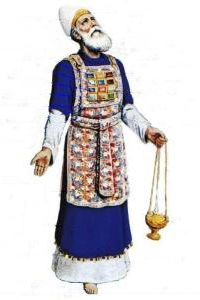
\includegraphics[width=50mm,scale=1.5]{Extras/Melchisedec.jpg}
\vspace{0.4in}  % Create a title for the document and write it in bold font
\LARGE{\textbf{\date}} % Again, do a line break
\linebreak 
% Create a subtitle \large{with Outlines, Statistics, Cross References, and Notes}
\vspace{0.5in}
\begin{flushleft}
\LARGE{Day \#76: Thursday, 17  March 2022  \\}\vspace{0.25in}
\LARGE{Judges 10-12 Psalm 76 Proverb 17}
\end{flushleft}
\vspace{0.6in}
\bigskip

\normalsize{Xenia, Oh.\\}
\normalsize{created: \today}
\vspace{1.3in}

\end{flushright}
\end{titlepage}

\newpage 
\tableofcontents\hypertarget{TOC}{}
\listoffigures
\listoftables

\hyphenation{A-bim-e-lech bre-thren E-phra-im  Gib-e-o-nites Jer-u-sa-lem through-out Phil-i-stines The-o-phil-us Am-a-le-kites ven-geance Mesh-el-e-mi-ah onan-ism Phar-a-oh thoughts grev-ous-ness Hach-a-liah adul-ter-er Shad-rach}

%%%%%%%%%%%%%%%%% EXTRA COLORS
%%%%%%%%%%%%%%%%% EXTRA COLORS
%%%%%%%%%%%%%%%%% EXTRA COLORS
\definecolor{champagne}{rgb}{0.97,0.91,0.81}
\definecolor{bone}{rgb}{0.89,0.85,0.79}

\definecolor{ForestGreen}{rgb}{0.00,0.29,0.098}
\definecolor{GIVING}{cmyk}{1,0.0,0.72,.1}

\definecolor{MLPE}{cmyk}{1,1,0,.45}
\definecolor{SOCCER}{cmyk}{.77, 0, .42, .49}
\definecolor{PAYBILL}{cmyk}{0,0.83,0.76,0.07}
\definecolor{SERMON}{cmyk}{.14,.9,0,.30} % aka seance \href{http://www.flatuicolorpicker.com/purple-cmyk-color-model/}{seance}
\definecolor{BIBLE}{cmyk}{0,.17,.74,.17}
\definecolor{WORKBLUE}{cmyk}{1, .5, 0, .6}
\definecolor{myOrange}{cmyk}{0, .4, .98, .03}
\definecolor{myTan}{cmyk}{0.0,.07,.17,.10}
\definecolor{myRed}{cmyk}{0,1,1,0}
\definecolor{myWhite}{cmyk}{0,0,0,0}
\definecolor{BLUESoD}{cmyk}{.97,.84,0,.04}
\definecolor{WHITE}{cmyk}{0,0,0,0}
\definecolor{OLDGOLD}{cmyk}{0.05,0.3,1.00,0}
\definecolor{CASTLETON}{cmyk}{1,0,0.31,0.66}
\definecolor{cadmiumgreen}{rgb}{0.0, 0.42, 0.24}
\definecolor{jungle}{rgb}{0.203,0.4882,0.1718}
\definecolor{MYGOLD}{rgb}{1,.84,0}

\definecolor{MYLIGHTGRAY}{rgb}{.85,.85,.85}

\definecolor{codegreen}{rgb}{0,0.6,0}
\definecolor{codegray}{rgb}{0.5,0.5,0.5}
\definecolor{codepurple}{rgb}{0.58,0,0.82}
\definecolor{backcolour}{rgb}{0.95,0.95,0.92}


\mdfdefinestyle{MyFrame}{%
    linecolor=blue,
    outerlinewidth=2pt,
    roundcorner=5pt,
    innertopmargin=\baselineskip,
    innerbottommargin=\baselineskip,
    innerrightmargin=10pt,
    innerleftmargin=10pt,
    backgroundcolor=gray!25!white}


\mdfdefinestyle{MyFrame2}{%
    linecolor=black,
    outerlinewidth=2pt,
    roundcorner=5pt,
    innertopmargin=\baselineskip,
    innerbottommargin=\baselineskip,
    innerrightmargin=10pt,
    innerleftmargin=10pt,
    backgroundcolor=yellow!25!white}


%%%%%
%% for PFTTIS list
%%%%%

%%% And Joseph said unto
\index[PFTTIS]{And Joseph said unto!Genesis!Gen 40:008}
\index[PFTTIS]{And Joseph said unto!Genesis!Gen 40:012}
\index[PFTTIS]{And Joseph said unto!Genesis!Gen 41:025}
\index[PFTTIS]{And Joseph said unto!Genesis!Gen 42:014}
\index[PFTTIS]{And Joseph said unto!Genesis!Gen 42:018}
\index[PFTTIS]{And Joseph said unto!Genesis!Gen 44:015}
\index[PFTTIS]{And Joseph said unto!Genesis!Gen 45:003}
\index[PFTTIS]{And Joseph said unto!Genesis!Gen 45:004}
\index[PFTTIS]{And Joseph said unto!Genesis!Gen 46:031}
\index[PFTTIS]{And Joseph said unto!Genesis!Gen 48:009}
\index[PFTTIS]{And Joseph said unto!Genesis!Gen 48:018}
\index[PFTTIS]{And Joseph said unto!Genesis!Gen 50:019}
\index[PFTTIS]{And Joseph said unto!Genesis!Gen 50:024}


%%% a shadow
\index[PFTTIS]{a shadow!1Chronicles!1Chr 029:15}
\index[PFTTIS]{a shadow!Job!Job 008:09}
\index[PFTTIS]{a shadow!Job!Job 014:02}
\index[PFTTIS]{a shadow!Job!Job 017:07}
\index[PFTTIS]{a shadow!Psalm!Psa 102:011}
\index[PFTTIS]{a shadow!Psalm!Psa 144:004}
\index[PFTTIS]{a shadow!Ecclesiastes!Eccl 006:012}
\index[PFTTIS]{a shadow!Ecclesiastes!Eccl 008:013}
\index[PFTTIS]{a shadow!Isaiah!Isa 04:006}
\index[PFTTIS]{a shadow!Isaiah!Isa 25:004}
\index[PFTTIS]{a shadow!Jonah!Jnh 04:06}
\index[PFTTIS]{a shadow!Colossians!Col 02:017}
\index[PFTTIS]{a shadow!Hebews!Heb 10:001}

%%% blessed is the man
\index[PFTTIS]{blessed is the man!Psalm!Psa 001:001}
\index[PFTTIS]{blessed is the man!Psalm!Psa 032:002}
\index[PFTTIS]{blessed is the man!Psalm!Psa 034:008}
\index[PFTTIS]{blessed is the man!Psalm!Psa 065:004}
\index[PFTTIS]{blessed is the man!Psalm!Psa 084:005}
\index[PFTTIS]{blessed is the man!Psalm!Psa 084:012}
\index[PFTTIS]{blessed is the man!Psalm!Psa 094:012}
\index[PFTTIS]{blessed is the man!Psalm!Psa 112:001}
\index[PFTTIS]{blessed is the man!Proverbs!Pro 008:034}
\index[PFTTIS]{blessed is the man!Isaiah!Isa 056:002}
\index[PFTTIS]{blessed is the man!Jeremiah!Jer 017:007}
\index[PFTTIS]{blessed is the man!Romans!Rom 004:008}
\index[PFTTIS]{blessed is the man!James!Jam 001:012}


%%% carry them
\index[PFTTIS]{carry them!Leviticus!Lev 14:045}
\index[PFTTIS]{carry them!Numbers!Num 11:012}
\index[PFTTIS]{carry them!Joshua!Jsh 04:003}
\index[PFTTIS]{carry them!1Samuel!1Sam 20:040}
\index[PFTTIS]{carry them!1Kings!1Kng 08:046}
\index[PFTTIS]{carry them!2Chronicles!2Chr 06:036}
\index[PFTTIS]{carry them!Ezra!Ezra 05:015}
\index[PFTTIS]{carry them!Isaiah!Isa 40:011}
\index[PFTTIS]{carry them!Isaiah!Isa 41:016}
\index[PFTTIS]{carry them!Isaiah!Isa 57:013}
\index[PFTTIS]{carry them!Jeremiah!Jer 20:004}
\index[PFTTIS]{carry them!Jeremiah!Jer 20:005}
\index[PFTTIS]{carry them!Jeremiah!Jer 43:012}


\index[PFTTIS]{good tidings!2Samuel!2Sam 18:027}
\index[PFTTIS]{good tidings!1Kings!1Ki 01:042}
\index[PFTTIS]{good tidings!2Kings!2Ki 07:009 (2x)}
\index[PFTTIS]{good tidings!Isaiah!Isa 40:009 (2x)}
\index[PFTTIS]{good tidings!Isaiah!Isa 41:007}
\index[PFTTIS]{good tidings!Isaiah!Isa 52:007}
\index[PFTTIS]{good tidings!Isaiah!Isa 61:001}
\index[PFTTIS]{good tidings!Nahum!Nah 01:005}
\index[PFTTIS]{good tidings!Luke!Lk 02:010}
\index[PFTTIS]{good tidings!1Thessalonians!1Thess 03:006}


%%% dead body
\index[PFTTIS]{dead body!Leviticus!Lev 21:011}
\index[PFTTIS]{dead body!Numbers!Num 06:006}
\index[PFTTIS]{dead body!Numbers!Num 09:006}
\index[PFTTIS]{dead body!Numbers!Num 09:007}
\index[PFTTIS]{dead body!Numbers!Num 09:010}
\index[PFTTIS]{dead body!Numbers!Num 09:011}
\index[PFTTIS]{dead body!Numbers!Num 09:013}
\index[PFTTIS]{dead body!Numbers!Num 09:016}
\index[PFTTIS]{dead body!2Kings!2Ki 08:005}
\index[PFTTIS]{dead body!Isaiah!Isa 26:019}
\index[PFTTIS]{dead body!Jeremiah!Jer 26:023}
\index[PFTTIS]{dead body!Jeremiah!Jer 36:030}
\index[PFTTIS]{dead body!Haggai!Hag 02:013}

%%% great sea
\index[PFTTIS]{great sea!Numbers!Num 34:006}
\index[PFTTIS]{great sea!Numbers!Num 34:007}
\index[PFTTIS]{great sea!Joshua!Jos 01:004}
\index[PFTTIS]{great sea!Joshua!Jos 09:001}
\index[PFTTIS]{great sea!Joshua!Jos 15:012}
\index[PFTTIS]{great sea!Joshua!Jos 15:047}
\index[PFTTIS]{great sea!Joshua!Jos 23:004}
\index[PFTTIS]{great sea!Ezekiel!Eze 47:010}
\index[PFTTIS]{great sea!Ezekiel!Eze 47:015}
\index[PFTTIS]{great sea!Ezekiel!Eze 47:019}
\index[PFTTIS]{great sea!Ezekiel!Eze 47:020}
\index[PFTTIS]{great sea!Ezekiel!Eze 48:028}
\index[PFTTIS]{great sea!Daniel!Dan 07:002}


%%% have forsaken me
\index[PFTTIS]{have forsaken me!Judges!Jdg 10:013}
\index[PFTTIS]{have forsaken me!1Samuel!1Sam 08:008}
\index[PFTTIS]{have forsaken me!1Kings!1Ki 11:033}
\index[PFTTIS]{have forsaken me!2Kings!2Ki 22:017}
\index[PFTTIS]{have forsaken me!2Chronicles!2Chr 12:005}
\index[PFTTIS]{have forsaken me!2Chronicles!2Chr 34:025}
\index[PFTTIS]{have forsaken me!Jeremiah!Jer 01:016}
\index[PFTTIS]{have forsaken me!Jeremiah!Jer 02:013}
\index[PFTTIS]{have forsaken me!Jeremiah!Jer 05:007}
\index[PFTTIS]{have forsaken me!Jeremiah!Jer 05:019}
\index[PFTTIS]{have forsaken me!Jeremiah!Jer 16:011 (2x)}
\index[PFTTIS]{have forsaken me!Jeremiah!Jer 19:004}

%%% no king
\index[PFTTIS]{no king!Judges!Jdg 17:06}
\index[PFTTIS]{no king!Judges!Jdg 18:01}
\index[PFTTIS]{no king!Judges!Jdg 19:01}
\index[PFTTIS]{no king!Judges!Jdg 21:25}
\index[PFTTIS]{no king!1Kings!1Ki 22:47}
\index[PFTTIS]{no king!2Kings!2Ki 23:25}
\index[PFTTIS]{no king!Nehemiah!Neh 13:26}
\index[PFTTIS]{no king!Psalms!Psa 033:016}
\index[PFTTIS]{no king!Proverbs!Pro 30:27}
\index[PFTTIS]{no king!Daniel!Dan 02:10}
\index[PFTTIS]{no king!Hosea!Hos 10:03}
\index[PFTTIS]{no king!Micah!Mic 04:09}
\index[PFTTIS]{no king!John!Jhn 19:15}


%%% rebellious house
\index[PFTTIS]{rebellious house!Exodus!Exo 02:005}
\index[PFTTIS]{rebellious house!Exodus!Exo 02:006}
\index[PFTTIS]{rebellious house!Exodus!Exo 02:008}
\index[PFTTIS]{rebellious house!Exodus!Exo 03:009}
\index[PFTTIS]{rebellious house!Exodus!Exo 03:026}
\index[PFTTIS]{rebellious house!Exodus!Exo 03:027}
\index[PFTTIS]{rebellious house!Exodus!Exo 12:002 (2x)}
\index[PFTTIS]{rebellious house!Exodus!Exo 12:003}
\index[PFTTIS]{rebellious house!Exodus!Exo 12:009}
\index[PFTTIS]{rebellious house!Exodus!Exo 12:025}
\index[PFTTIS]{rebellious house!Exodus!Exo 17:012}
\index[PFTTIS]{rebellious house!Exodus!Exo 24:003}

%%% seek him
\index[PFTTIS]{seek him!Deuteronomy!Deu 04:029}\index[PFTTIS]{seek him!1Samuel!1Sam 23:025}
\index[PFTTIS]{seek him!1Chronicles!1Chr 28:009}
\index[PFTTIS]{seek him!2Chronicles!1Chr 15:002}
\index[PFTTIS]{seek him!Ezra!Ezr 08:022}
\index[PFTTIS]{seek him!Psalms!Psa 022:026}
\index[PFTTIS]{seek him!Psalms!Psa 024:006}
\index[PFTTIS]{seek him!Psalms!Psa 119:002}
\index[PFTTIS]{seek him!SoS!SoS 03:002}
\index[PFTTIS]{seek him!SoS!SoS 06:001}
\index[PFTTIS]{seek him!Hosea!Hos 07:010}
\index[PFTTIS]{seek him!Amos!Amo 05:008}
\index[PFTTIS]{seek him!Hebrews!Heb 11:0063}


%%% seek ye
\index[PFTTIS]{seek ye!Isaiah!Isa 34:016}
\index[PFTTIS]{seek ye!Isaiah!Isa 45:019}
\index[PFTTIS]{seek ye!Isaiah!Isa 55:006}
\index[PFTTIS]{seek ye!Amos!Amos 5:004}
\index[PFTTIS]{seek ye!John!John 1:38}
\index[PFTTIS]{seek ye!John!John 18:4}
\index[PFTTIS]{seek ye!John!John 18:7}
\index[PFTTIS]{seek ye!Matthew!Matt 6:33}
\index[PFTTIS]{seek ye!Numbers!Num 16:10}
\index[PFTTIS]{seek ye!Luke!Luke 12:31}
\index[PFTTIS]{seek ye!Luke!Luke 24:5}
\index[PFTTIS]{seek ye!Psalm!Psa 27:8}
\index[PFTTIS]{seek ye!Zephaniah!Zeph 2:3}

%%% the uncircumcised
\index[PFTTIS]{the uncircumcised!Genesis!Gen 17:014}
\index[PFTTIS]{the uncircumcised!Judges!Jdg 14:003}
\index[PFTTIS]{the uncircumcised!Judges!Jdg 15:018}
\index[PFTTIS]{the uncircumcised!2Samuel!2Sam 01:020}
\index[PFTTIS]{the uncircumcised!Isaiah!Isa 02:001}
\index[PFTTIS]{the uncircumcised!Jeremiah!Jer 09:025}
\index[PFTTIS]{the uncircumcised!Ezekiel!Eze 28:010}
\index[PFTTIS]{the uncircumcised!Ezekiel!Eze 31:018}
\index[PFTTIS]{the uncircumcised!Ezekiel!Eze 32:019}
\index[PFTTIS]{the uncircumcised!Ezekiel!Eze 32:027}
\index[PFTTIS]{the uncircumcised!Ezekiel!Eze 32:028}
\index[PFTTIS]{the uncircumcised!Ezekiel!Eze 32:029}
\index[PFTTIS]{the uncircumcised!Ezekiel!Eze 32:032}

%%% worship him
\index[PFTTIS]{worship him!Psalms!Psa 97:007}
\index[PFTTIS]{worship him!Zephaniah!Zeph 02:011}
\index[PFTTIS]{worship him!Matthew!Matt 02:002}
\index[PFTTIS]{worship him!Matthew!Matt 02:008}
\index[PFTTIS]{worship him!John!John 04:023}
\index[PFTTIS]{worship him!John!John 04:024 (2x)} 
\index[PFTTIS]{worship him!Acts!Acts 17:023}
\index[PFTTIS]{worship him!Hebrews!Heb 01:006}
\index[PFTTIS]{worship him!Revelation!Rev 04:010}
\index[PFTTIS]{worship him!Revelation!Rev 13:008}
\index[PFTTIS]{worship him!Revelation!Rev 14:007}
\index[PFTTIS]{worship him!Revelation!Rev 19:010}


%%%%%
%% for PFTTIS list
%%%%%

%%% afflictions
\index[WFTTIS]{afflictions!Psalms!Psa 34:019}
\index[WFTTIS]{afflictions!Psalms!Psa 132:001}
\index[WFTTIS]{afflictions!Acts!Acts 07:010}
\index[WFTTIS]{afflictions!Acts!Acts 20:023}
\index[WFTTIS]{afflictions!2Corinthians!2Cor 06:004}
\index[WFTTIS]{afflictions!Colossians!Col 01:024}
\index[WFTTIS]{afflictions!1Thessalonians!1Thess 03:003}
\index[WFTTIS]{afflictions!2Timothy!2Tim 01:008}
\index[WFTTIS]{afflictions!2Timothy!2Tim 03:011}
\index[WFTTIS]{afflictions!2Timothy!2Tim 04:005}
\index[WFTTIS]{afflictions!Hebrews!Heb 10:032}
\index[WFTTIS]{afflictions!Hebrews!Heb 10:033}
\index[WFTTIS]{afflictions!1Peter!1Pet 05:009}

%%% acsend
\index[WFTTIS]{acsend!Joshua!Jos 06:05}
\index[WFTTIS]{acsend!Psalm!Psa 024:003}
\index[WFTTIS]{acsend!Psalm!Psa 135:007}
\index[WFTTIS]{acsend!Psalm!Psa 139:008}
\index[WFTTIS]{acsend!Isaiah!Isa 14:013}
\index[WFTTIS]{acsend!Isaiah!Isa 14:014}
\index[WFTTIS]{acsend!Jeremiah!Jer 10:013}
\index[WFTTIS]{acsend!Jeremiah!Jer 51:016}
\index[WFTTIS]{acsend!Ezekiel!Eze 38:009}
\index[WFTTIS]{acsend!John!John 06:062}
\index[WFTTIS]{acsend!John!John 20:017}
\index[WFTTIS]{acsend!Romans!Rom 10:006}
\index[WFTTIS]{acsend!Revelation!Rev 17:008}

%%% Assyrian
\index[WFTTIS]{Assyrian!Isaiah!Isa 10:005}
\index[WFTTIS]{Assyrian!Isaiah!Isa 10:024}
\index[WFTTIS]{Assyrian!Isaiah!Isa 14:025}
\index[WFTTIS]{Assyrian!Isaiah!Isa 19:023}
\index[WFTTIS]{Assyrian!Isaiah!Isa 23:013}
\index[WFTTIS]{Assyrian!Isaiah!Isa 30:031}
\index[WFTTIS]{Assyrian!Isaiah!Isa 31:008}
\index[WFTTIS]{Assyrian!Isaiah!Isa 52:004}
\index[WFTTIS]{Assyrian!Ezekiel!Eze 31:003}
\index[WFTTIS]{Assyrian!Hosea!Hos 05:013}
\index[WFTTIS]{Assyrian!Hosea!Hos 11:005}
\index[WFTTIS]{Assyrian!Micah!Hos 05:005}
\index[WFTTIS]{Assyrian!Micah!Hos 05:006}

%%% blot
\index[WFTTIS]{blot!Exodus!Exo 32:032}
\index[WFTTIS]{blot!Exodus!Exo 32:033}
\index[WFTTIS]{blot!Numbers!Num 05:026}
\index[WFTTIS]{blot!Deuteronomy!Deut 09:014}
\index[WFTTIS]{blot!Deuteronomy!Deut 25:019}
\index[WFTTIS]{blot!Deuteronomy!Deut 29:020}
\index[WFTTIS]{blot!2Kings!2Ki 14:027}
\index[WFTTIS]{blot!Job!Job 31:007}
\index[WFTTIS]{blot!Psalms!Psa 51:001}
\index[WFTTIS]{blot!Psalms!Psa 51:009}
\index[WFTTIS]{blot!Proverbs!Pro 09:007}
\index[WFTTIS]{blot!Jeremiah!Jer 18:023}
\index[WFTTIS]{blot!Revelation!Rev 03:005}


%%% chain
\index[WFTTIS]{chain!Genesis!Gen 41:042}
\index[WFTTIS]{chain!1Kings!1Ki 07:017}
\index[WFTTIS]{chain!Psalms!Psa 73:006}
\index[WFTTIS]{chain!SoS!Sos 04:009}
\index[WFTTIS]{chain!Lamentations!Lam 03:007}
\index[WFTTIS]{chain!Ezekiel!Eze 07:023}
\index[WFTTIS]{chain!Ezekiel!Eze 16:011}
\index[WFTTIS]{chain!Daniel!Dan 05:007}
\index[WFTTIS]{chain!Daniel!Dan 05:016}
\index[WFTTIS]{chain!Daniel!Dan 05:029}
\index[WFTTIS]{chain!Acts!Acts 28:020}
\index[WFTTIS]{chain!2Timothy!2Tim 01:016}
\index[WFTTIS]{chain!Revelation!Rev 20:001}


%%% controversy
\index[WFTTIS]{controversy!Deuteronomy!Deu 17:008}
\index[WFTTIS]{controversy!Deuteronomy!Deu 19:017}
\index[WFTTIS]{controversy!Deuteronomy!Deu 21:005}
\index[WFTTIS]{controversy!Deuteronomy!Deu 25:001}
\index[WFTTIS]{controversy!2Samuel!2Sam 15:002}
\index[WFTTIS]{controversy!Isaiah!Isa 34:008}
\index[WFTTIS]{controversy!Jeremiah!Jer 25:031}
\index[WFTTIS]{controversy!Ezekiel!Eze 44:024}
\index[WFTTIS]{controversy!Hosea!Hos 04:001}
\index[WFTTIS]{controversy!Hosea!Hos 12:002}
\index[WFTTIS]{controversy!Micah!Mic 06:002 (2x)}
\index[WFTTIS]{controversy!1Timothy!1Tim 03:016}


%%% Dagon/Dagon's
\index[WFTTIS]{Dagon!Judges!Jdg 16:023}
\index[WFTTIS]{Dagon!1Samuel!1Sam 05:002 (2x)}
\index[WFTTIS]{Dagon!1Samuel!1Sam 05:003 (2x)}
\index[WFTTIS]{Dagon!1Samuel!1Sam 05:004 (3x)}
\index[WFTTIS]{Dagon!1Samuel!1Sam 05:005 (3x)}
\index[WFTTIS]{Dagon!1Samuel!1Sam 05:007}
\index[WFTTIS]{Dagon!1Chronicles!1Chr 10:010}

%%% disobedient
\index[WFTTIS]{disobedient!1Kings!1Ki 13:026}
\index[WFTTIS]{disobedient!Nehemiah!Neh 09:026}
\index[WFTTIS]{disobedient!Luke!Luke 01:017}
\index[WFTTIS]{disobedient!Acts!Acts 26:019}
\index[WFTTIS]{disobedient!Romans!Rom 01:030}
\index[WFTTIS]{disobedient!Romans!Rom 10:021}
\index[WFTTIS]{disobedient!1Timothy!1Tim 01:009}
\index[WFTTIS]{disobedient!2Timothy!2Tim 03:002}
\index[WFTTIS]{disobedient!Titus!Titus 01:016}
\index[WFTTIS]{disobedient!Titus!Titus 03:003}
\index[WFTTIS]{disobedient!1Peter!1Pet 02:007}
\index[WFTTIS]{disobedient!1Peter!1Pet 02:008}
\index[WFTTIS]{disobedient!1Peter!1Pet 03:020}


%%% doubt
\index[WFTTIS]{doubt!Genesis!Gen 37:033}
\index[WFTTIS]{doubt!Deuteronomy!Deu 28:066}
\index[WFTTIS]{doubt!Job!Job 12:002}
\index[WFTTIS]{doubt!Matthew!Matt 14:031}
\index[WFTTIS]{doubt!Matthew!Matt 21:021}
\index[WFTTIS]{doubt!Mark!Mk 11:023}
\index[WFTTIS]{doubt!Luke!Lk 11:020}
\index[WFTTIS]{doubt!John!Jhn 10:024}
\index[WFTTIS]{doubt!Acts!Acts 02:012}
\index[WFTTIS]{doubt!Acts!Acts 28:004}
\index[WFTTIS]{doubt!1Corinthians!1Cor 09:010}
\index[WFTTIS]{doubt!Galatians!Gal 04:020}
\index[WFTTIS]{doubt!1John!1Jhn 02:019}


%%% dungeon
\index[WFTTIS]{dungeon!Genesis!Gen 40:015}
\index[WFTTIS]{dungeon!Genesis!Gen 41:014}
\index[WFTTIS]{dungeon!Exodus!Exo 12:029}
\index[WFTTIS]{dungeon!Jeremiah!Jer 37:016}
\index[WFTTIS]{dungeon!Jeremiah!Jer 38:006 (2x)}
\index[WFTTIS]{dungeon!Jeremiah!Jer 38:007}
\index[WFTTIS]{dungeon!Jeremiah!Jer 38:009}
\index[WFTTIS]{dungeon!Jeremiah!Jer 38:010}
\index[WFTTIS]{dungeon!Jeremiah!Jer 38:011}
\index[WFTTIS]{dungeon!Jeremiah!Jer 38:013}
\index[WFTTIS]{dungeon!Lamentations!Lam 03:053}
\index[WFTTIS]{dungeon!Lamentations!Lam 03:055}


%%% error
\index[WFTTIS]{error!2Samuel!2Sam 06:007}
\index[WFTTIS]{error!Job!Job 19:004}
\index[WFTTIS]{error!Ecclesiastes!Ecc 05:006}
\index[WFTTIS]{error!Ecclesiastes!Ecc 10:005}
\index[WFTTIS]{error!Isaiah!Isa 32:006}
\index[WFTTIS]{error!Daniel!Dan 06:004}
\index[WFTTIS]{error!Matthew!Matt 27:064}
\index[WFTTIS]{error!Romans!Rom 01:027}
\index[WFTTIS]{error!James!Jam 05:020}
\index[WFTTIS]{error!2Peter!2Pet 02:018}
\index[WFTTIS]{error!2Peter!2Pet 03:017}
\index[WFTTIS]{error!1John!1Jn 04:006}
\index[WFTTIS]{error!Jude!Jude 01:011}

%%% fourish
\index[WFTTIS]{fourish!Psalms!Psa 072:007}
\index[WFTTIS]{fourish!Psalms!Psa 072:016}
\index[WFTTIS]{fourish!Psalms!Psa 092:007}
\index[WFTTIS]{fourish!Psalms!Psa 092:012}
\index[WFTTIS]{fourish!Psalms!Psa 092:013}
\index[WFTTIS]{fourish!Psalms!Psa 132:018}
\index[WFTTIS]{fourish!Proverbs!Pro 11:28}
\index[WFTTIS]{fourish!Proverbs!Pro 14:11}
\index[WFTTIS]{fourish!Ecclesiastes!Ecc 12:05}
\index[WFTTIS]{fourish!SongOfSolomon!SOS 07:12}
\index[WFTTIS]{fourish!Isaiah!Isa 17:11}
\index[WFTTIS]{fourish!Isaiah!Isa 66:14}
\index[WFTTIS]{fourish!Ezekiel!Eze 17:24}




%%% giants
\index[WFTTIS]{giants!Genesis!Gen 06:004}
\index[WFTTIS]{giants!Numbers!Num 13:033}
\index[WFTTIS]{giants!Deuteronomy!Deut 02:011}
\index[WFTTIS]{giants!Deuteronomy!Deut 02:021}
\index[WFTTIS]{giants!Deuteronomy!Deut 03:011}
\index[WFTTIS]{giants!Deuteronomy!Deut 03:013}
\index[WFTTIS]{giants!Joshua!Josh 12:004}
\index[WFTTIS]{giants!Joshua!Josh 13:012}
\index[WFTTIS]{giants!Joshua!Josh 15:008}
\index[WFTTIS]{giants!Joshua!Josh 17:015}
\index[WFTTIS]{giants!Joshua!Josh 16:016}

%%% good man
\index[WFTTIS]{good man!2 Samuel!2Sa 18:27}
%(1) Psalms 37:23 [5]
%(1) Psalms 112:5 [2]
%(1) Proverbs 12:2 [2]
%(1) Proverbs 13:22 [2]
%(1) Proverbs 14:14 [14]
%(1) Micah 7:2 [2]
%(1) Matthew 12:35 [2]
%(1) Luke 6:45 [2]
%(1) Luke 23:50 [15]
%(1) John 7:12 [17]
%(1) Acts 11:24 [5]
%(1) Romans 5:7 [14]

%%% Hinnom
\index[WFTTIS]{Hinnom!Joshua!Jsh 15:008}
\index[WFTTIS]{Hinnom!Joshua!Jsh 18:016}
\index[WFTTIS]{Hinnom!2Kings!2Ki 23:010}
\index[WFTTIS]{Hinnom!2Chronicles!2Chr 28:003}
\index[WFTTIS]{Hinnom!2Chronicles!2Chr 33:006}
\index[WFTTIS]{Hinnom!Nehemiah!Neh 11:030}
\index[WFTTIS]{Hinnom!Jeremiah!Jer 07:031}
\index[WFTTIS]{Hinnom!Jeremiah!Jer 07:032}
\index[WFTTIS]{Hinnom!Jeremiah!Jer 19:002}
\index[WFTTIS]{Hinnom!Jeremiah!Jer 19:006}
\index[WFTTIS]{Hinnom!Jeremiah!Jer 32:035}

%%% inclined
\index[WFTTIS]{inclined!Judges!Jdg 09:003}
\index[WFTTIS]{inclined!Psalms!Psa 040:001}
\index[WFTTIS]{inclined!Psalms!Psa 116:002}
\index[WFTTIS]{inclined!Psalms!Psa 119:112}
\index[WFTTIS]{inclined!Proverbs!Pro 05:13}
\index[WFTTIS]{inclined!Jeremiah!Jer 07:24}
\index[WFTTIS]{inclined!Jeremiah!Jer 07:26}
\index[WFTTIS]{inclined!Jeremiah!Jer 11:08}
\index[WFTTIS]{inclined!Jeremiah!Jer 17:23}
\index[WFTTIS]{inclined!Jeremiah!Jer 25:04}
\index[WFTTIS]{inclined!Jeremiah!Jer 34:14}
\index[WFTTIS]{inclined!Jeremiah!Jer 35:15}
\index[WFTTIS]{inclined!Jeremiah!Jer 44:05}


%%% laughed
\index[WFTTIS]{laughed!Genesis!Gen 17:017}
\index[WFTTIS]{laughed!Genesis!Gen 18:012}
\index[WFTTIS]{laughed!Genesis!Gen 18:015}
\index[WFTTIS]{laughed!2Kings!2Ki 19:021}
\index[WFTTIS]{laughed!2Chronicles!2Chr 30:010}
\index[WFTTIS]{laughed!Nehemiah!Neh 02:019}
\index[WFTTIS]{laughed!Job!Job 12:004}
\index[WFTTIS]{laughed!Job!Job 29:024}
\index[WFTTIS]{laughed!Isaiah!Isa 37:022}
\index[WFTTIS]{laughed!Ezekiel!Ezek 23:032}
\index[WFTTIS]{laughed!Matthew!Matt 09:024}
\index[WFTTIS]{laughed!Mark!Mk 05:040}
\index[WFTTIS]{laughed!Luke!Lk 08:053}

%%% liar
\index[WFTTIS]{liar!Job!Job 24:025}
\index[WFTTIS]{liar!Proverbs!Pro 17:004}
\index[WFTTIS]{liar!Proverbs!Pro 19:022}
\index[WFTTIS]{liar!Proverbs!Pro 30:006}
\index[WFTTIS]{liar!Jeremiah!Jer 15:018}
\index[WFTTIS]{liar!John!Jhn 08:044}
\index[WFTTIS]{liar!John!Jhn 08:055}
\index[WFTTIS]{liar!Romans!Rom 03:004}
\index[WFTTIS]{liar!1John!1Jhn 01:010}
\index[WFTTIS]{liar!1John!1Jhn 02:004}
\index[WFTTIS]{liar!1John!1Jhn 02:022}
\index[WFTTIS]{liar!1John!1Jhn 04:020}
\index[WFTTIS]{liar!1John!1Jhn 05:010}

%%% palsy
\index[WFTTIS]{palsy!Matthew!Matt 04:024}
\index[WFTTIS]{palsy!Matthew!Matt 08:006}
\index[WFTTIS]{palsy!Matthew!Matt 09:002}
\index[WFTTIS]{palsy!Matthew!Matt 09:006}
\index[WFTTIS]{palsy!Mark!Mk 02:003}
\index[WFTTIS]{palsy!Mark!Mk 02:004}
\index[WFTTIS]{palsy!Mark!Mk 02:005}
\index[WFTTIS]{palsy!Mark!Mk 02:009}
\index[WFTTIS]{palsy!Mark!Mk 02:010}
\index[WFTTIS]{palsy!Luke!Lk 05:018}
\index[WFTTIS]{palsy!Luke!Lk 05:024}
\index[WFTTIS]{palsy!Acts!Acts 09:033}

%%% Profitable
\index[WFTTIS]{profitable!Job!Job 22:002 (2x)}
\index[WFTTIS]{profitable!Ecclesiastes!Ecc 10:010}
\index[WFTTIS]{profitable!Isaiah!Isa 44:010}
\index[WFTTIS]{profitable!Jeremiah!Jer 13:007}
\index[WFTTIS]{profitable!Matthew!Matt 05:029}
\index[WFTTIS]{profitable!Matthew!Matt 05:030}
\index[WFTTIS]{profitable!Acts!Acts 20:020}
\index[WFTTIS]{profitable!1Timothy!1Tim 04:008}
\index[WFTTIS]{profitable!2Timothy!2Tim 03:016}
\index[WFTTIS]{profitable!2Timothy!2Tim 04:011}
\index[WFTTIS]{profitable!Titus!Titus 03:008}
\index[WFTTIS]{profitable!Philemon!Phlm 01:011}

%%% Rechab
\index[WFTTIS]{Rechab!2Samuel!2Sam 04:002}
\index[WFTTIS]{Rechab!2Samuel!2Sam 04:005}
\index[WFTTIS]{Rechab!2Samuel!2Sam 04:006}
\index[WFTTIS]{Rechab!2Samuel!2Sam 04:009}
\index[WFTTIS]{Rechab!2KIngs!2Ki 10:015}
\index[WFTTIS]{Rechab!2KIngs!2Ki 10:023}
\index[WFTTIS]{Rechab!1Chronicles!1Chr 02:055}
\index[WFTTIS]{Rechab!Nehemiah!Neh 03:014}
\index[WFTTIS]{Rechab!Jeremiah!Jer 35:006}
\index[WFTTIS]{Rechab!Jeremiah!Jer 35:008}
\index[WFTTIS]{Rechab!Jeremiah!Jer 35:014}
\index[WFTTIS]{Rechab!Jeremiah!Jer 35:016}
\index[WFTTIS]{Rechab!Jeremiah!Jer 35:019}

%%% serpents
\index[WFTTIS]{serpents!Exodus!Exo 07:012}
\index[WFTTIS]{serpents!Numbers!Num 21:006}
\index[WFTTIS]{serpents!Numbers!Num 21:007}
\index[WFTTIS]{serpents!Deuteronomy!Deu 08:015}
\index[WFTTIS]{serpents!Deuteronomy!Deu 32:024}
\index[WFTTIS]{serpents!Jeremiah!Jer 08:017}
\index[WFTTIS]{serpents!Matthew!Matt 10:016}
\index[WFTTIS]{serpents!Matthew!Matt 23:033}
\index[WFTTIS]{serpents!Mark!Mk 16:018}
\index[WFTTIS]{serpents!Luke!Lk 10:019}
\index[WFTTIS]{serpents!1Corinthians!1Cor 10:009}
\index[WFTTIS]{serpents!James!Jas 03:007}
\index[WFTTIS]{serpents!Revelation!Rev 09:019}

%%% short
\index[WFTTIS]{short!Numbers!Num 11:023}
\index[WFTTIS]{short!2Kings!2Ki 10:032}
\index[WFTTIS]{short!Job!Job 17:012}
\index[WFTTIS]{short!Job!Job 20:005}
\index[WFTTIS]{short!Psalms!Psa 89:047}
\index[WFTTIS]{short!Romans!Rom 03:023}
\index[WFTTIS]{short!Romans!Rom 09:028  (2x)}
\index[WFTTIS]{short!1Corinthians!1Cor 07:029}
\index[WFTTIS]{short!1Thessalonians!1Thess 02:017}
\index[WFTTIS]{short!Hebrews!Heb 04:001}
\index[WFTTIS]{short!Revelation!Rev 12:012}
\index[WFTTIS]{short!Revelation!Rev 17:010}

%%% smiteth
\index[WFTTIS]{smiteth!Exodus!Exo 21:012}
\index[WFTTIS]{smiteth!Exodus!Exo 21:15}
\index[WFTTIS]{smiteth!Deuteronomy!Dt 25:11}
\index[WFTTIS]{smiteth!Deuteronomy!Dt 27:24}
\index[WFTTIS]{smiteth!Joshua!Jsh 15:16}
\index[WFTTIS]{smiteth!Judges!Jdg 15:16}
\index[WFTTIS]{smiteth!2 Samuel!2Sa 05:08}
\index[WFTTIS]{smiteth!1Chronicles!1Chr 11:06}
\index[WFTTIS]{smiteth!Job!1Chr 26:12}
\index[WFTTIS]{smiteth!Isaiah!Isa 09:13}
\index[WFTTIS]{smiteth!Lamentations!Lam 03:30}
\index[WFTTIS]{smiteth!Ezekiel!Eze 07:09}
\index[WFTTIS]{smiteth!Luke!Lk 06:29}



%%% vanities
\index[WFTTIS]{vanities!Deuteronomy!Deut 21:021}
\index[WFTTIS]{vanities!1Kings!1Ki 16:013}
\index[WFTTIS]{vanities!1Kings!1Ki 16:026}
\index[WFTTIS]{vanities!Psalms!Psa 031:006}
\index[WFTTIS]{vanities!Ecclesiastes!Ecc 01:002 (2x)}
\index[WFTTIS]{vanities!Ecclesiastes!Ecc 05:007}
\index[WFTTIS]{vanities!Ecclesiastes!Ecc 12:008}
\index[WFTTIS]{vanities!Jeremiah!Jer 08:019}
\index[WFTTIS]{vanities!Jeremiah!Jer 10:008}
\index[WFTTIS]{vanities!Jeremiah!Jer 14:022}
\index[WFTTIS]{vanities!Jonah!Jnh 02:008}
\index[WFTTIS]{vanities!Acts!Acts 14:015}



%%%%%
%% for PFTTIS list
%%%%%

%%% worm
\index[WFITV]{worm!Exodus!Exo 16:024}
\index[WFITV]{worm!Job!Job 17:014}
\index[WFITV]{worm!Job!Job 24:029}
\index[WFITV]{worm!Job!Job 25:005 (2x)}
\index[WFITV]{worm!Psalms!Psa 022:006}
\index[WFITV]{worm!Isaiah!Isa 14:011}
\index[WFITV]{worm!Isaiah!Isa 41:014}
\index[WFITV]{worm!Isaiah!Isa 51:008}
\index[WFITV]{worm!Isaiah!Isa 66:024}
\index[WFITV]{worm!Jonah!Jnh 04:007}
\index[WFITV]{worm!Mark!Mk 09:044}
\index[WFITV]{worm!Mark!Mk 09:046}
\index[WFITV]{worm!Mark!Mk 09:048}


%\subsubsection{Title}
%\textbf{Introduction:} Isaiah 46 
%\index[speaker]{Speaker!Isaiah 49 (Title}
%\index[series]{Book (Speaker)!IPassage (Title)}
%\index[date]{2017/07/09!Isaiah 49 (Title)}
%\begin{compactenum}[I.]
%    \item  \textbf{Point} \index[scripture]{Isaiah!IPassage} (IPassage)
%\end{compactenum}




  


%\input{02OT-Exodus/ExodusIntroduction}

%\newpage
%\begin{figure}
%\begin{center}
%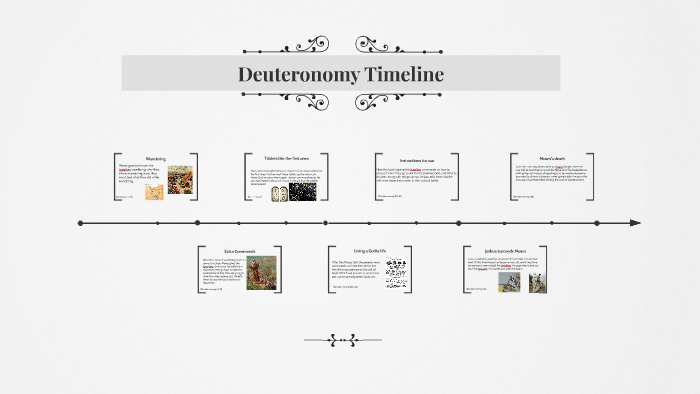
\includegraphics[scale=.7, angle=0]{05OT-Deuteronomy/References/AndrewSmithDeuteronomyTimeline.png}
%\caption[Deuteronomy Timeline by Andrew Smith]{Deuteronomy Timeline by Andrew %Smith}
%\label{fig:Deuteronomy Timeline by Andrew Smith}
%\end{center}
%\end{figure}

\newpage
\begin{figure}
\begin{center}
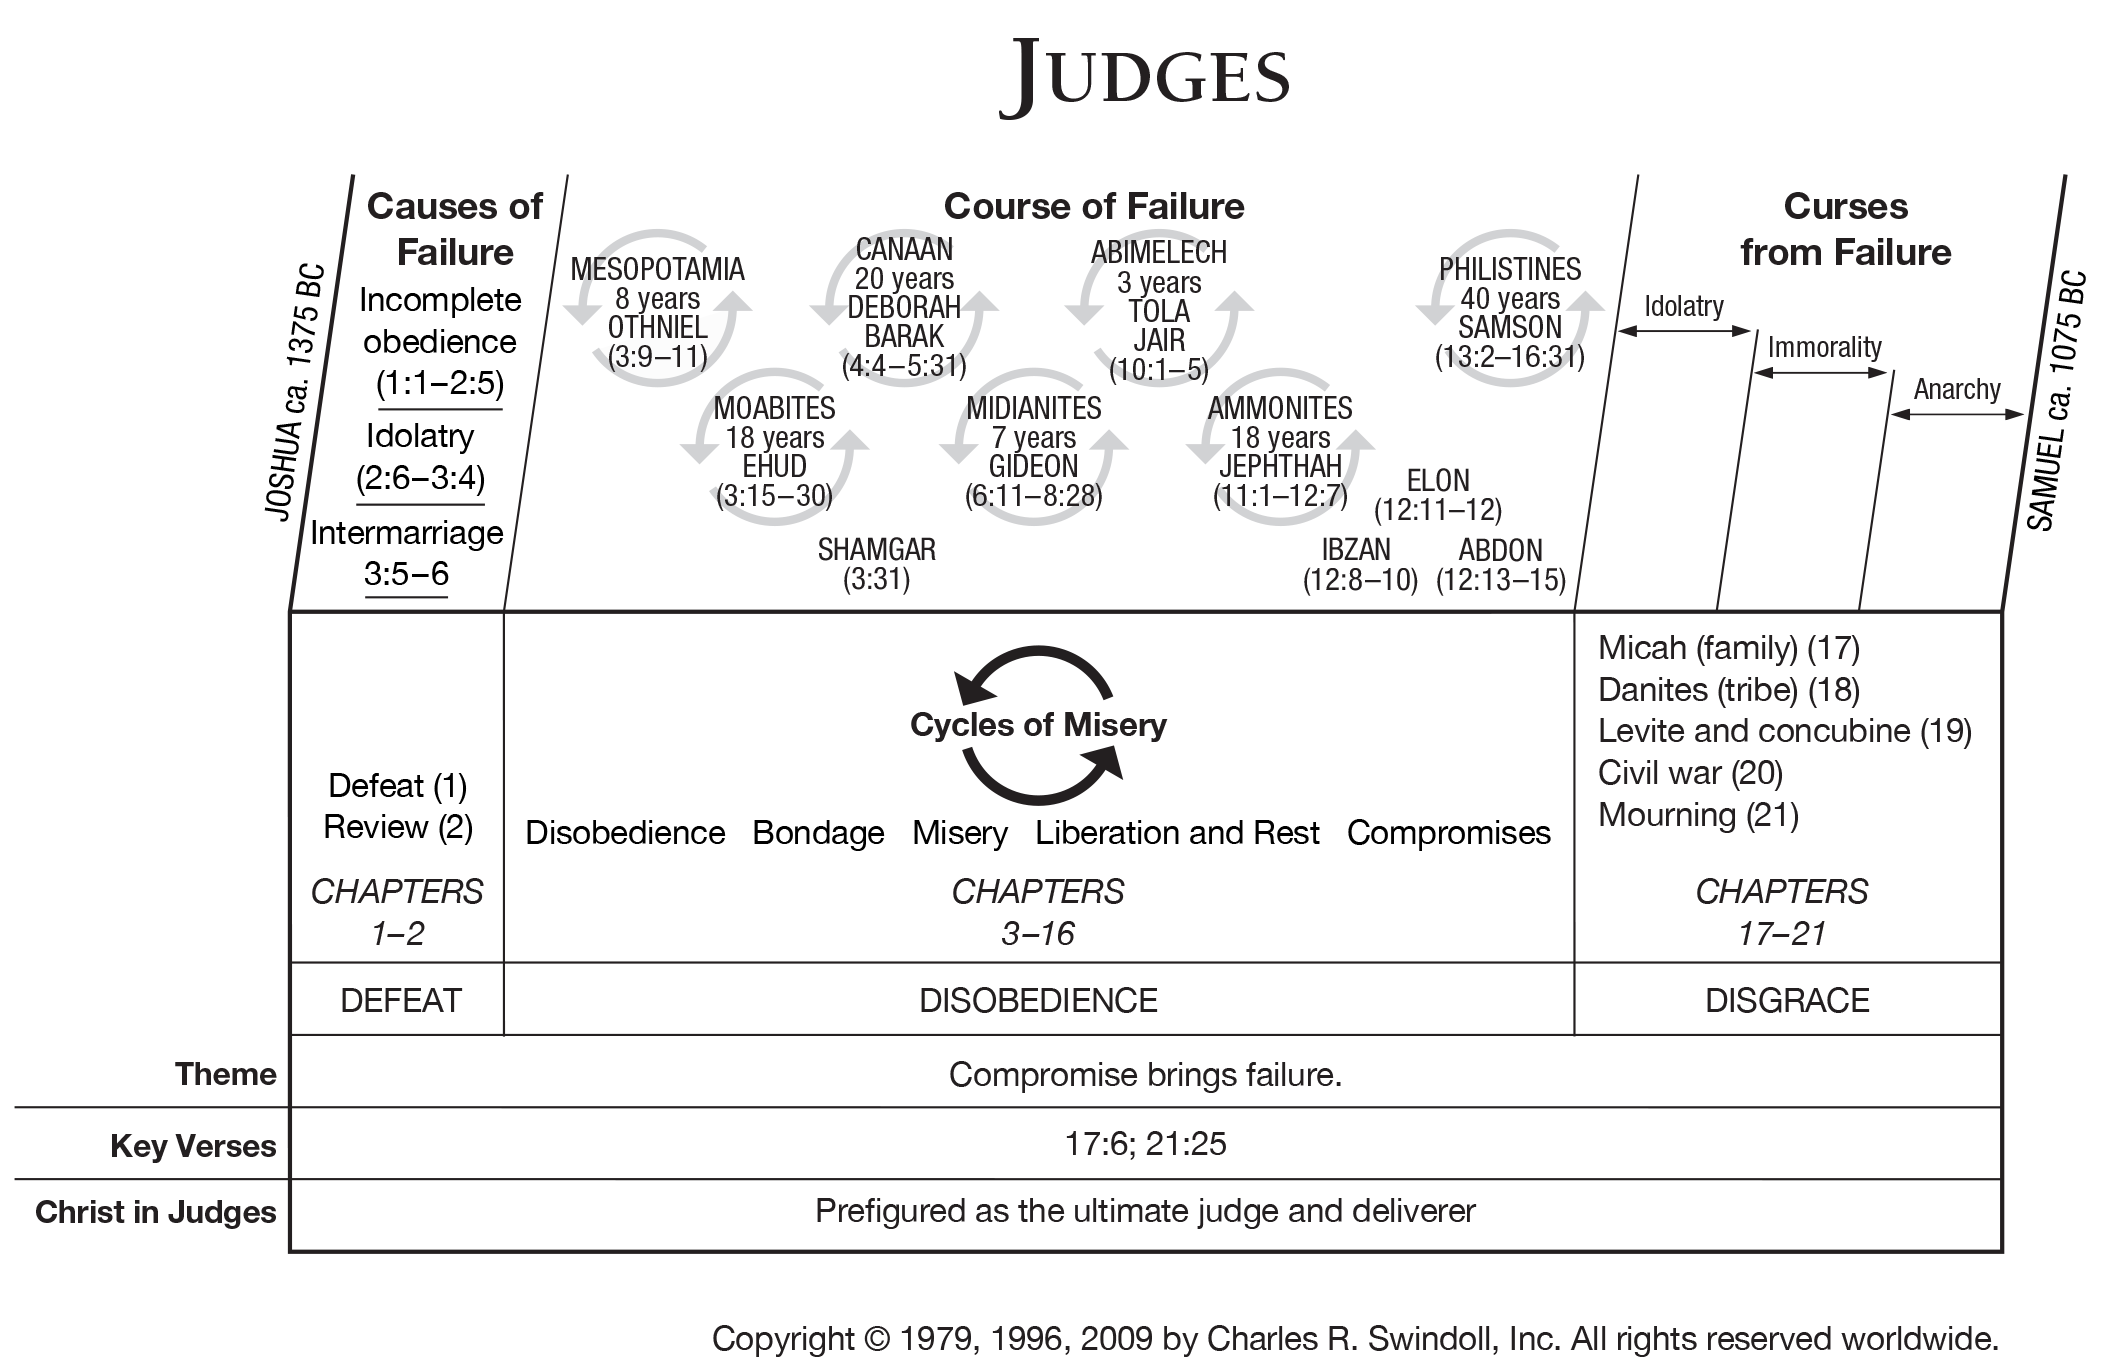
\includegraphics[scale=0.25, angle=90]{07OT-Judges/References/1.Judges-Swindoll}
\caption[Judges from Swindoll]{Judges from Swindoll}
\label{fig:Judges from Swindoll}
\end{center}
\end{figure}


%\newpage
%\begin{figure}
%\begin{center}
%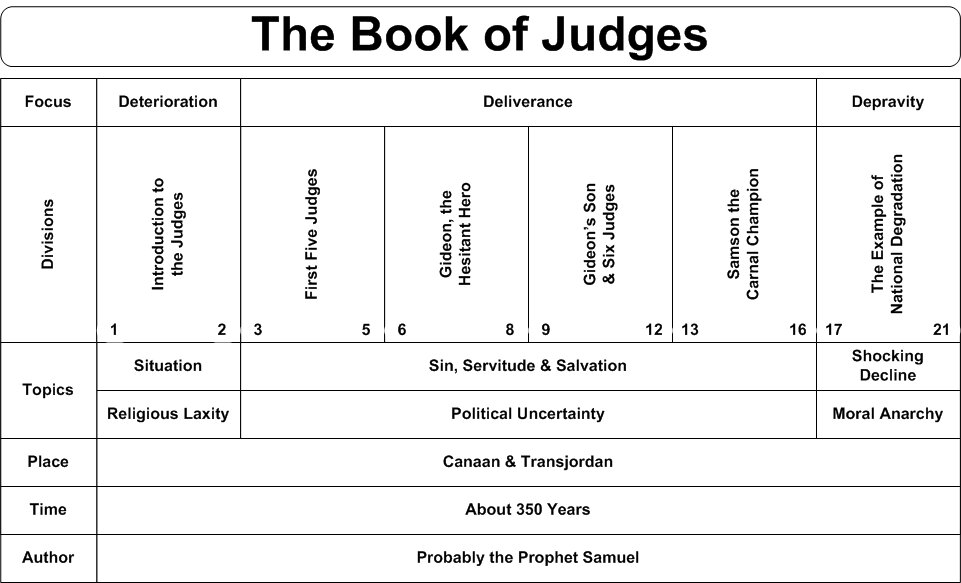
\includegraphics[scale=0.1, angle=0]{07OT-Judges/References/9.Swartzentrover-Judges}
%\caption[Judges from Swartzentrover]{Judges from Swartzentrover}
%\label{fig:Judges from Swartzentrover}
%\end{center}
%\end{figure}


\newpage
\begin{figure}
\begin{center}
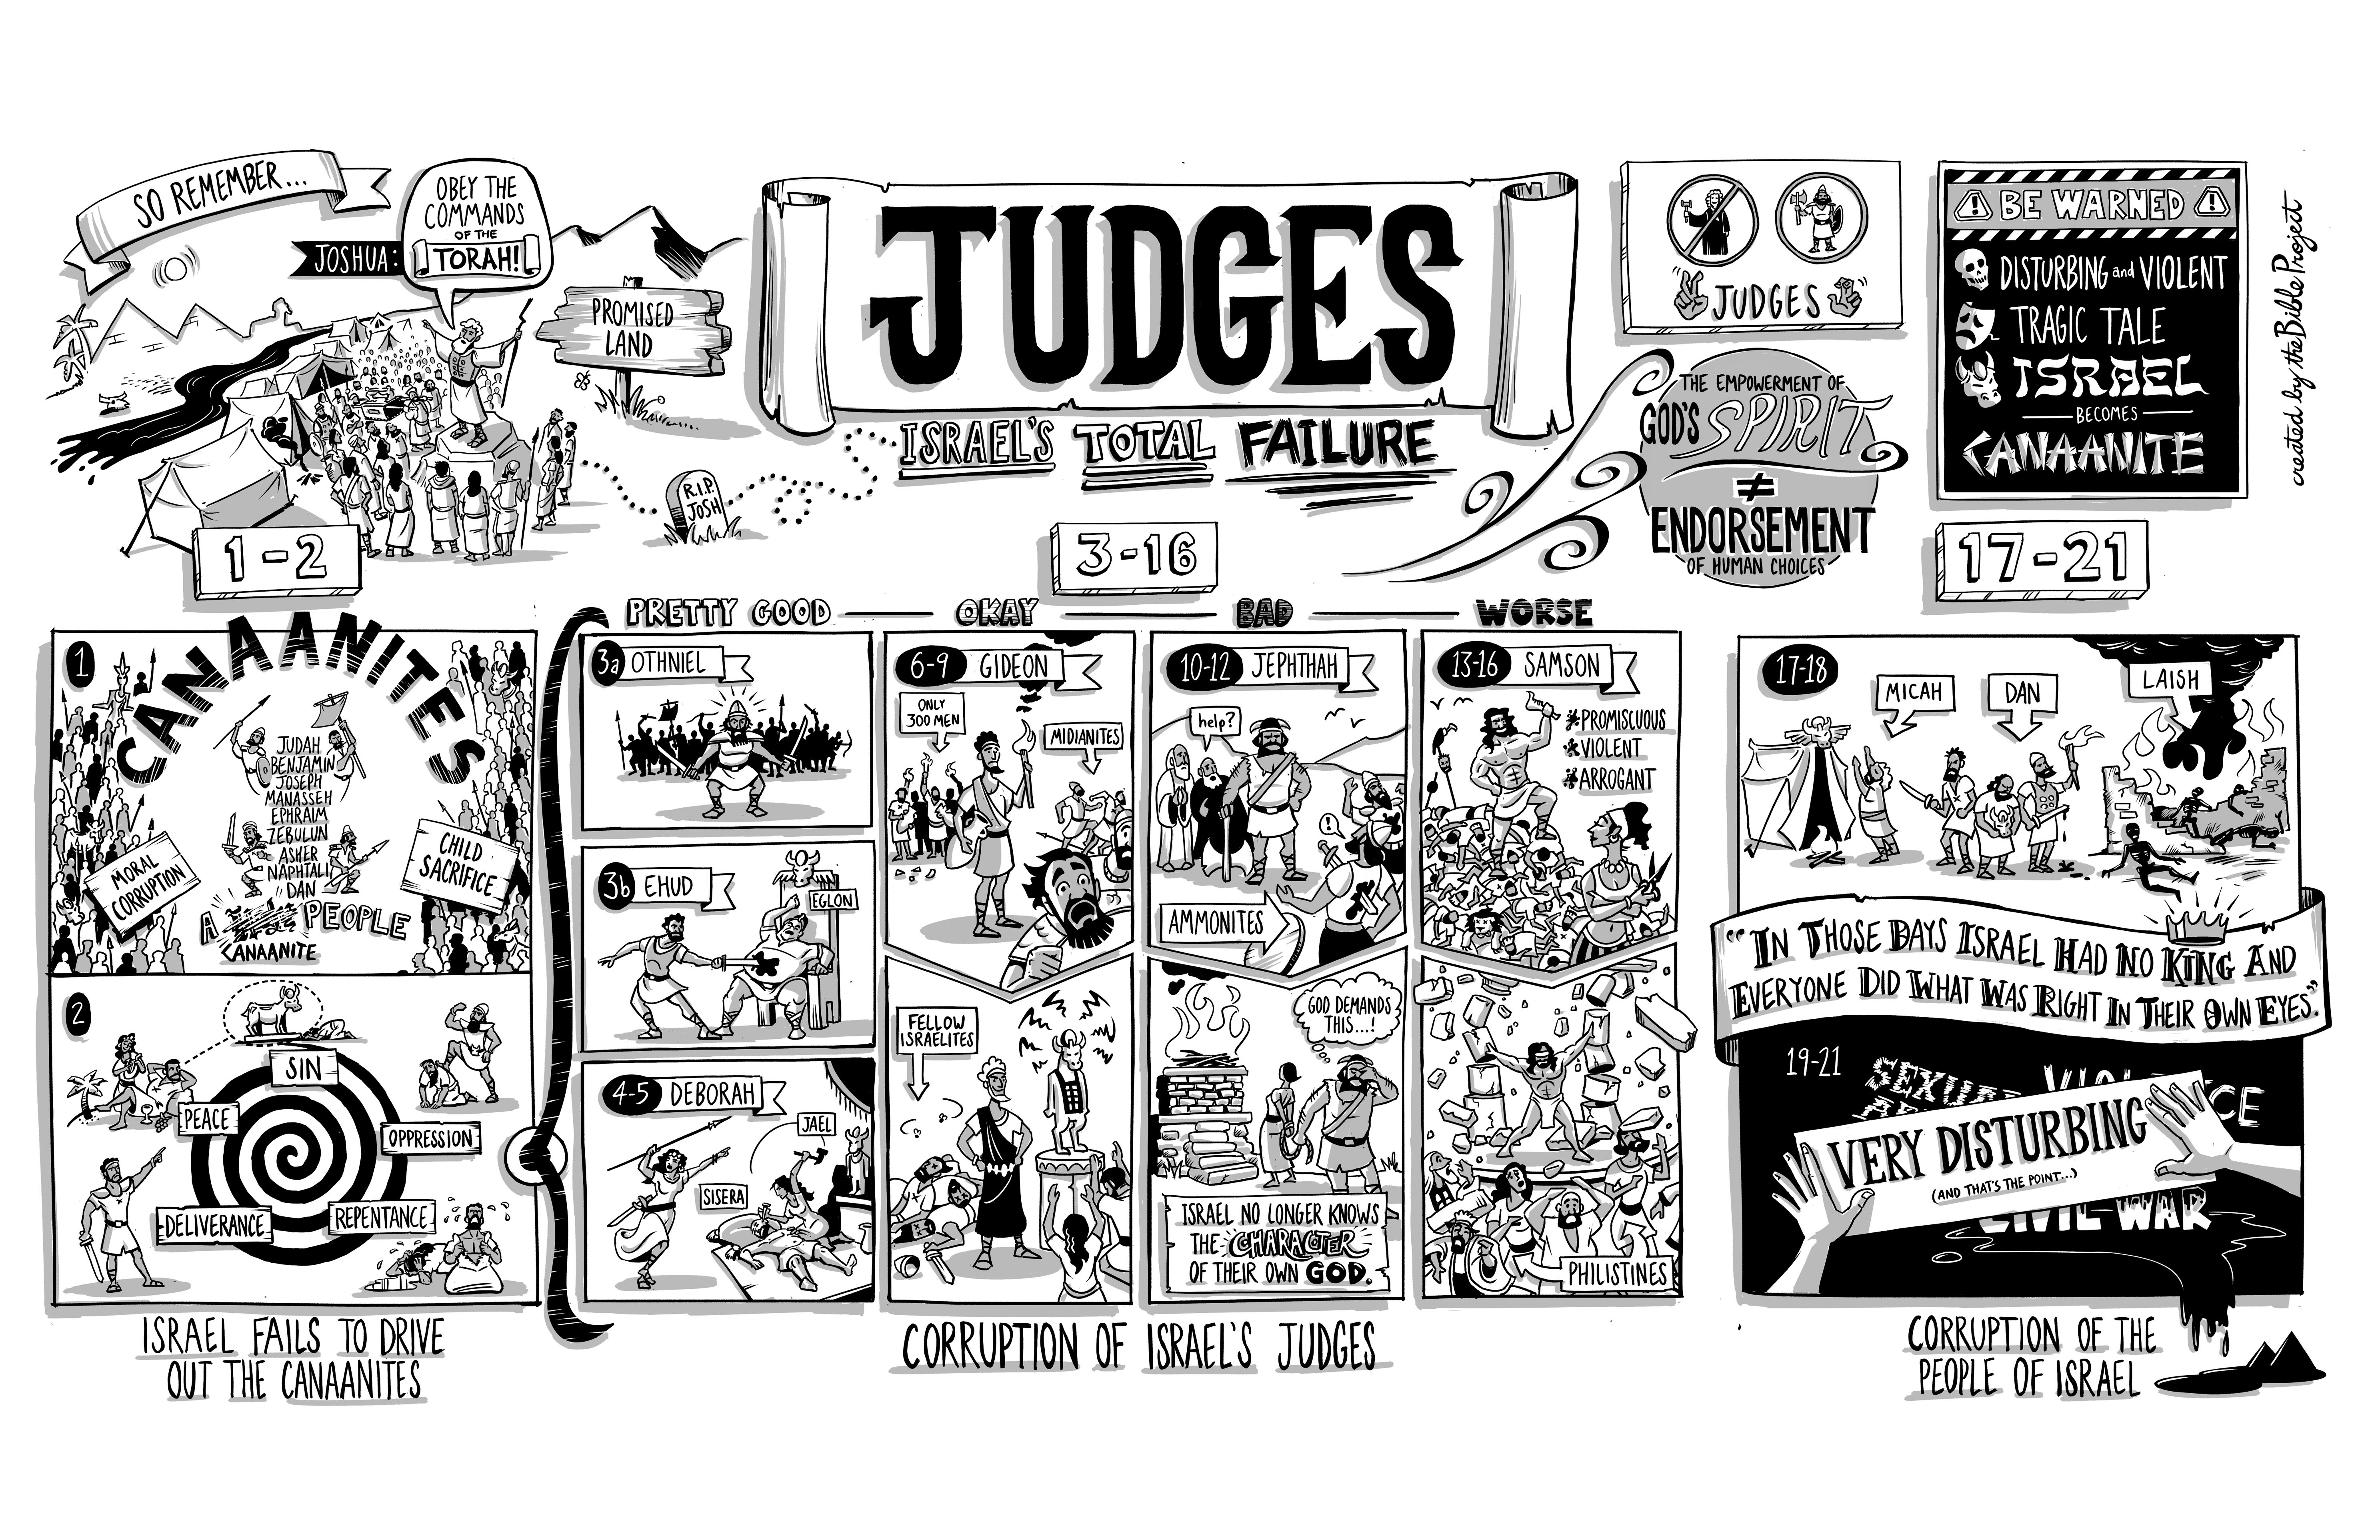
\includegraphics[scale=0.5, angle=90]{07OT-Judges/References/2.BibleProject-Judges}
\caption[Judges from the Bible Project]{Judges from the Bible Project}
\label{fig:Judges from the Bible Project}
\end{center}
\end{figure}


\newpage
\begin{figure}
\begin{center}
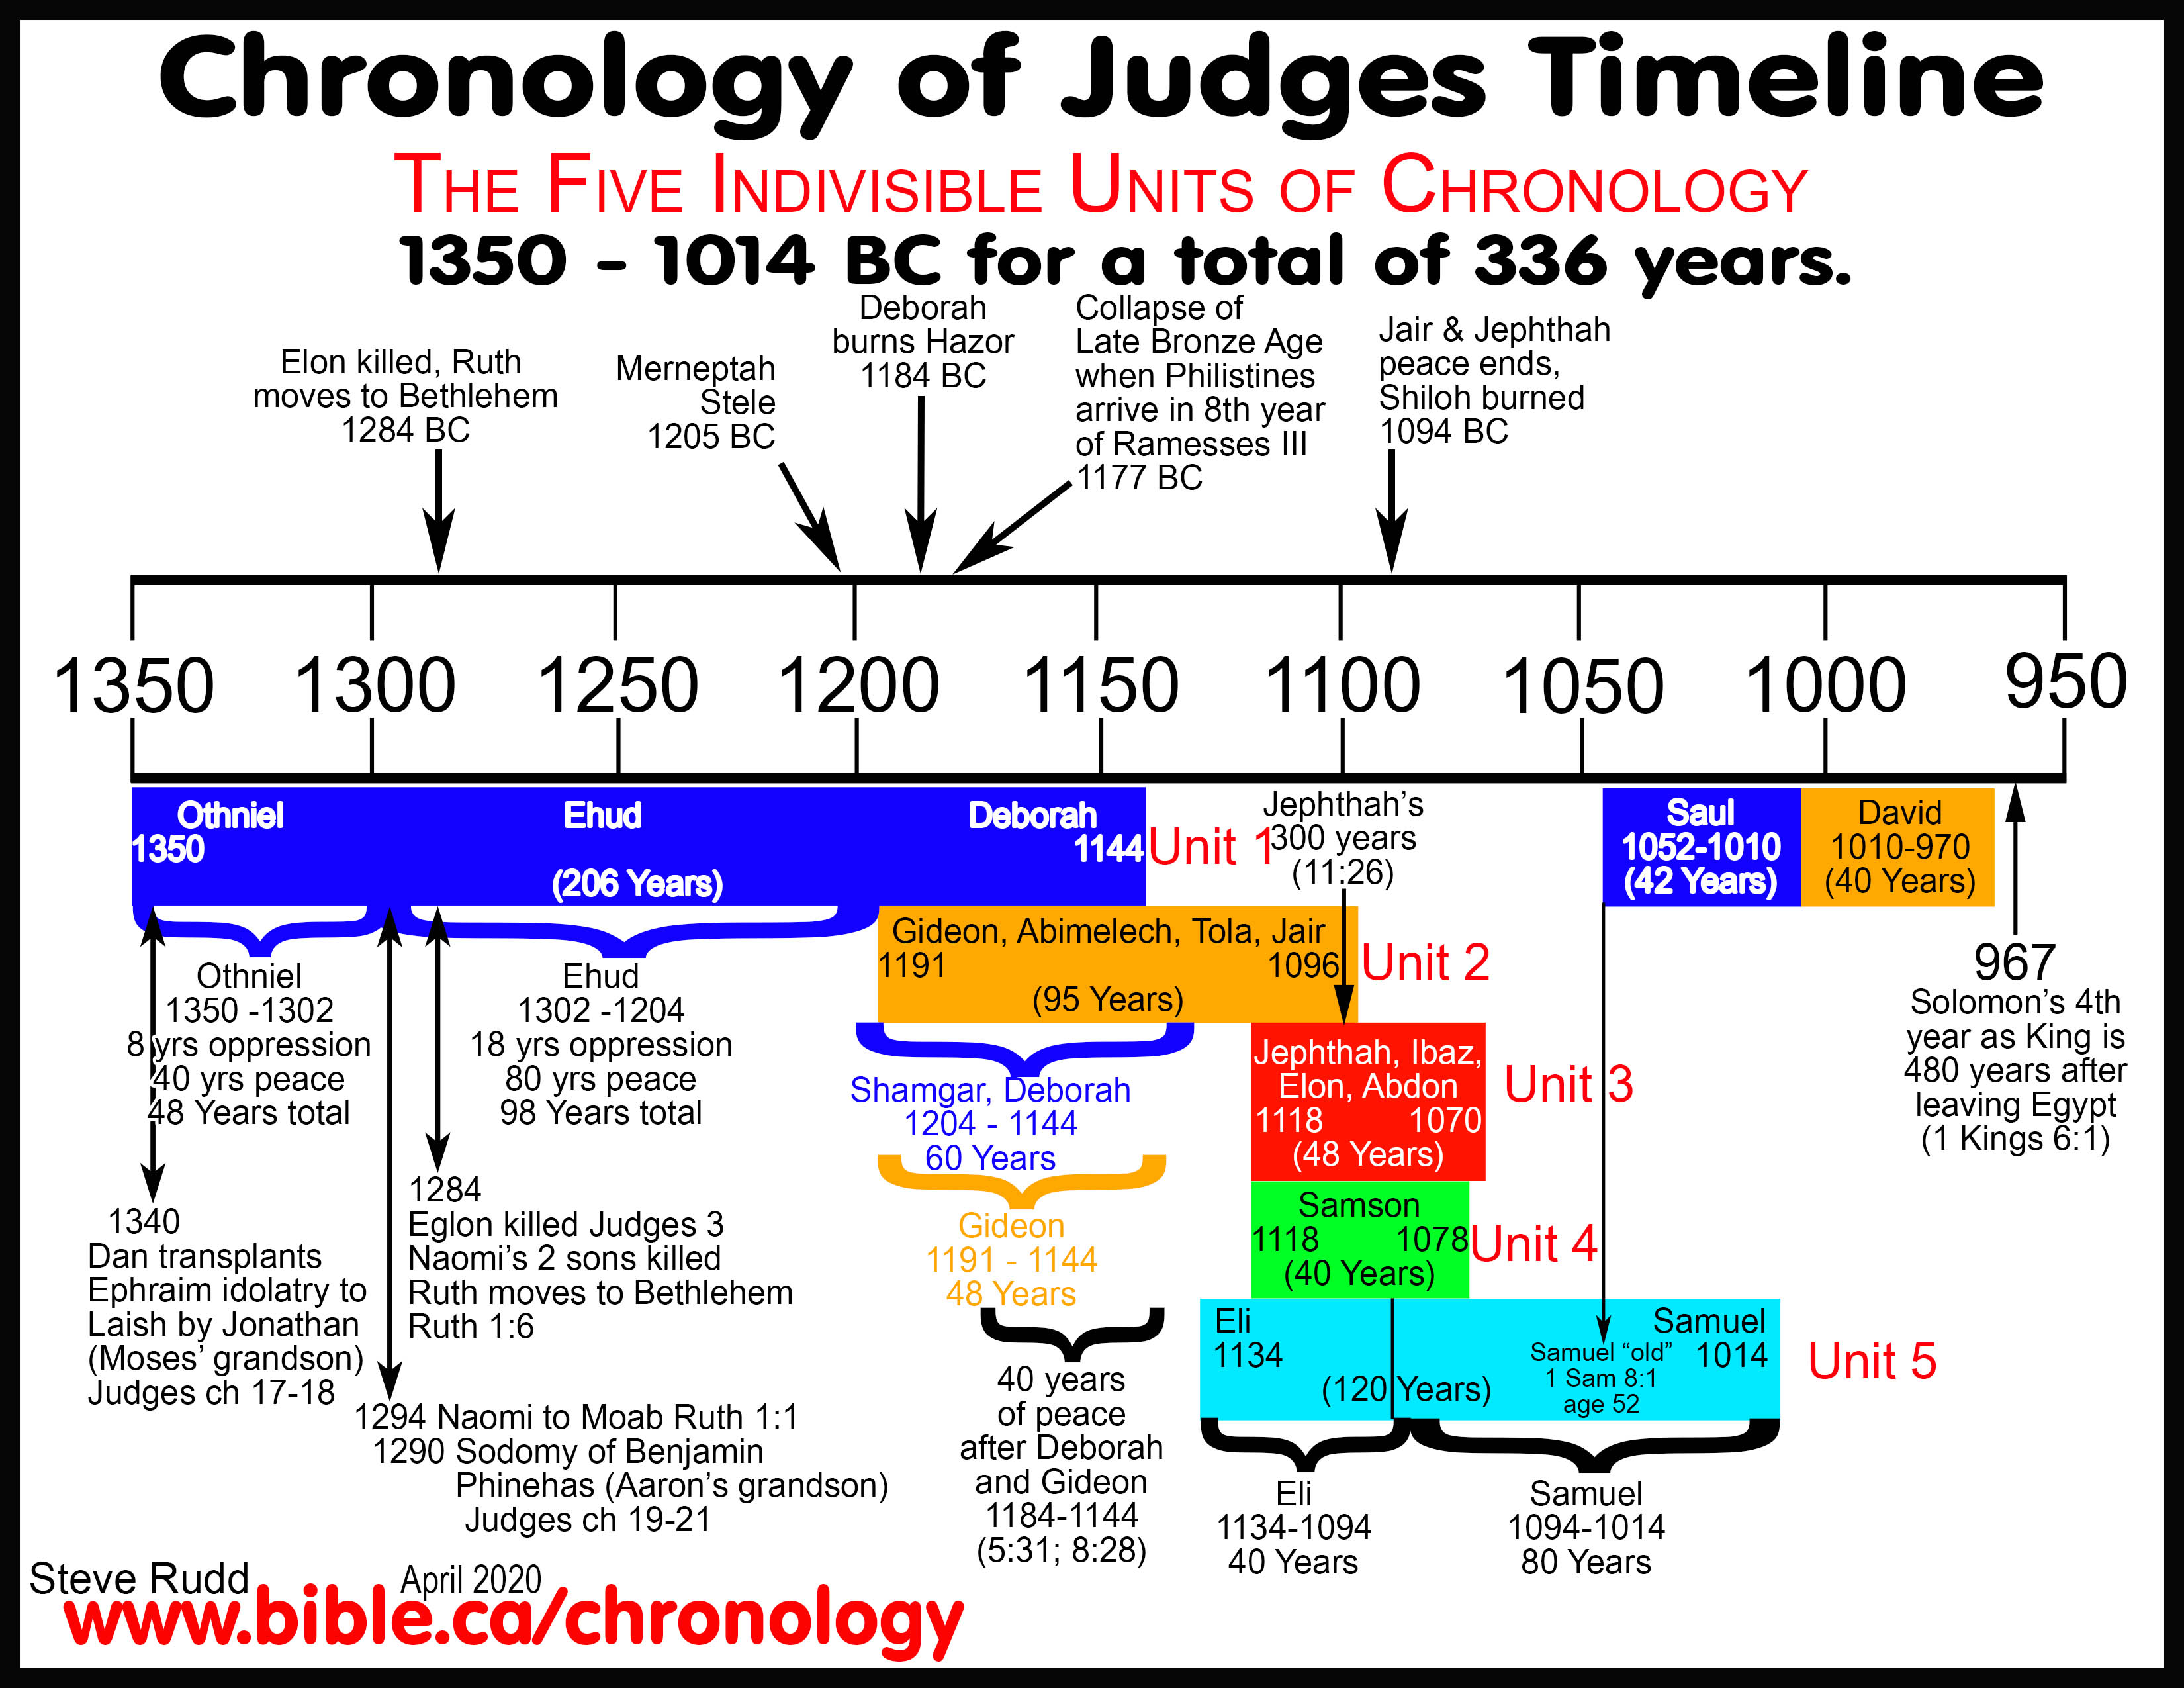
\includegraphics[scale=0.6, angle=90]{07OT-Judges/References/3.Chronology-Judges}
\caption[Chronology of Judges]{Chronology of Judges}
\label{fig:Chronology of Judges}
\end{center}
\end{figure}


\newpage
\begin{figure}
\begin{center}
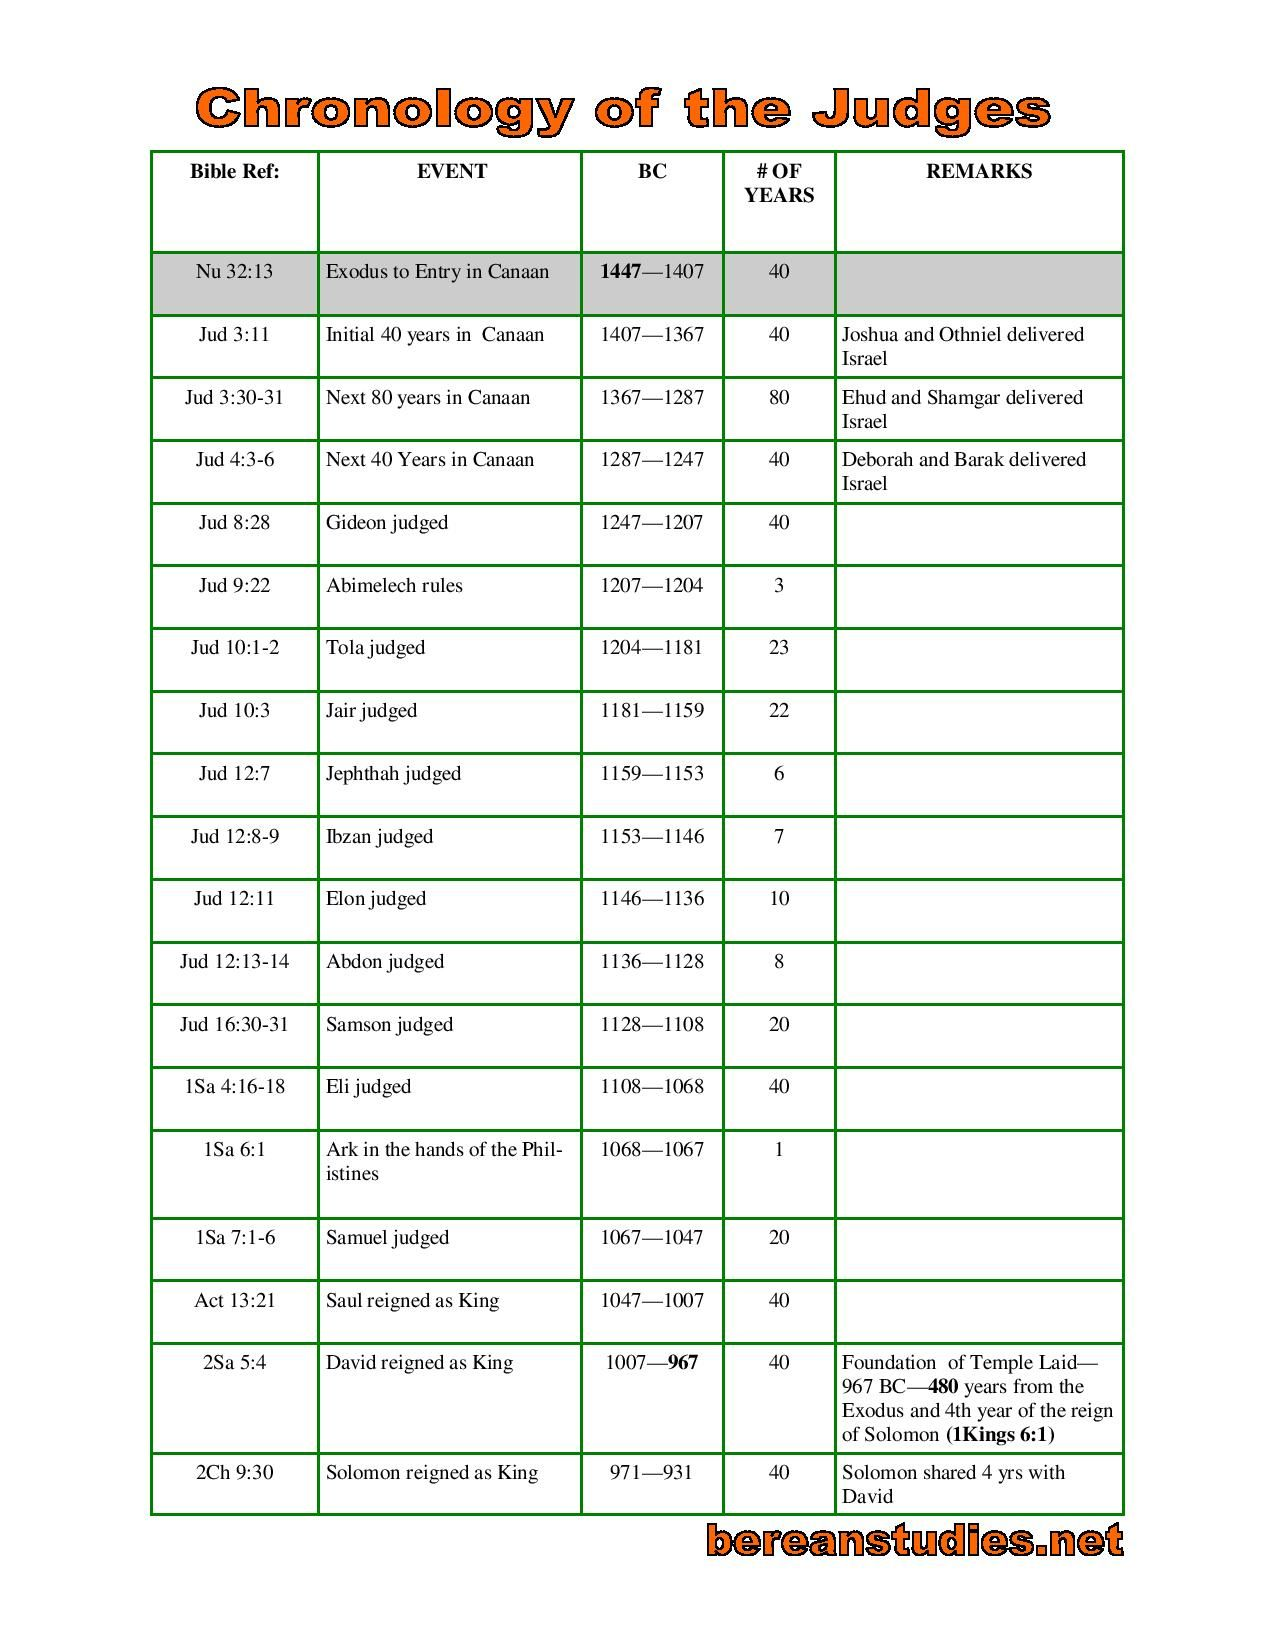
\includegraphics[scale=0.6, angle=0]{07OT-Judges/References/4.Chronology2-Judges}
\caption[Another Chronology of Judges]{Another Chronology of Judges}
\label{fig:Another Chronology of Judges}
\end{center}
\end{figure}

\newpage
\begin{figure}
\begin{center}
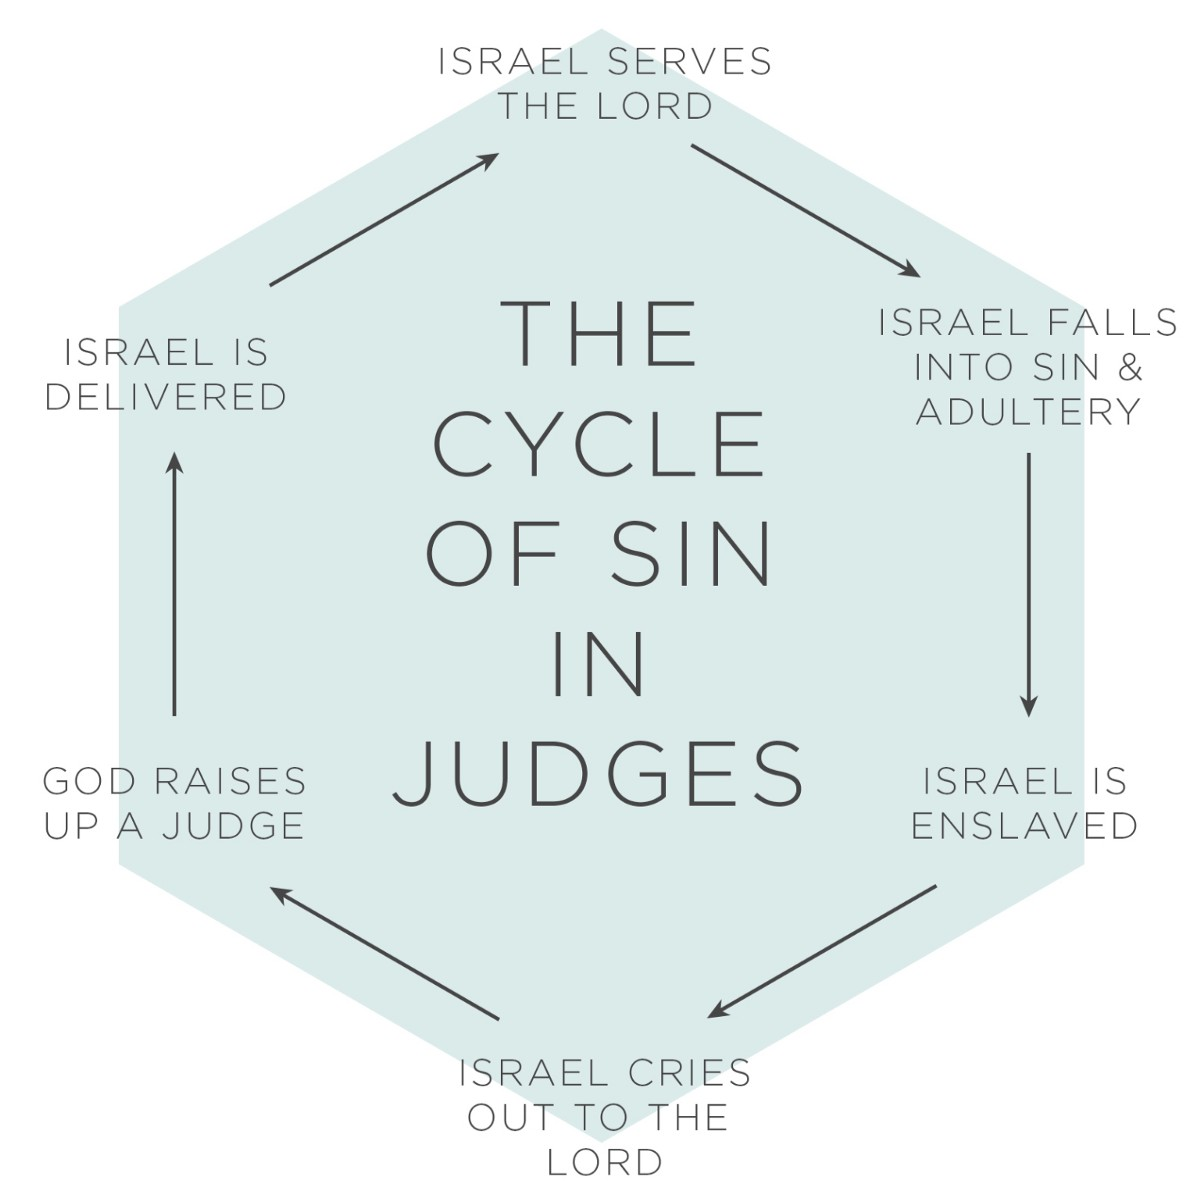
\includegraphics[scale=0.3, angle=0]{07OT-Judges/References/5.Cycles-Judges}
\caption[Cycle of Judges]{Cycle of Judges}
\label{fig:Cycle of Judges}
\end{center}
\end{figure}


\newpage
\begin{figure}
\begin{center}
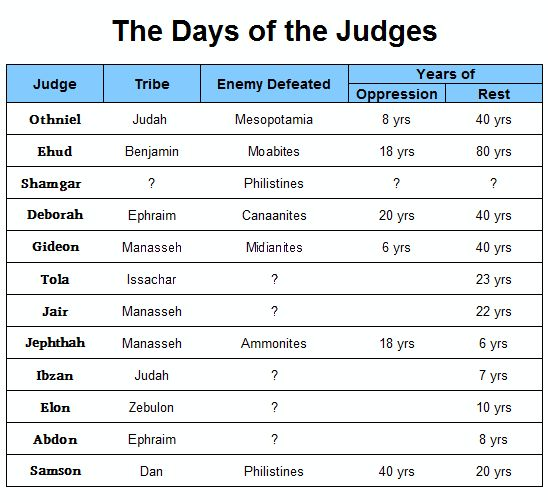
\includegraphics[scale=0.7, angle=0]{07OT-Judges/References/6.DaysOfJudges}
\caption[The Days of the Judges]{The Days of the Judges}
\label{fig:The Days of the Judges}
\end{center}
\end{figure}


\newpage
\begin{figure}
\begin{center}
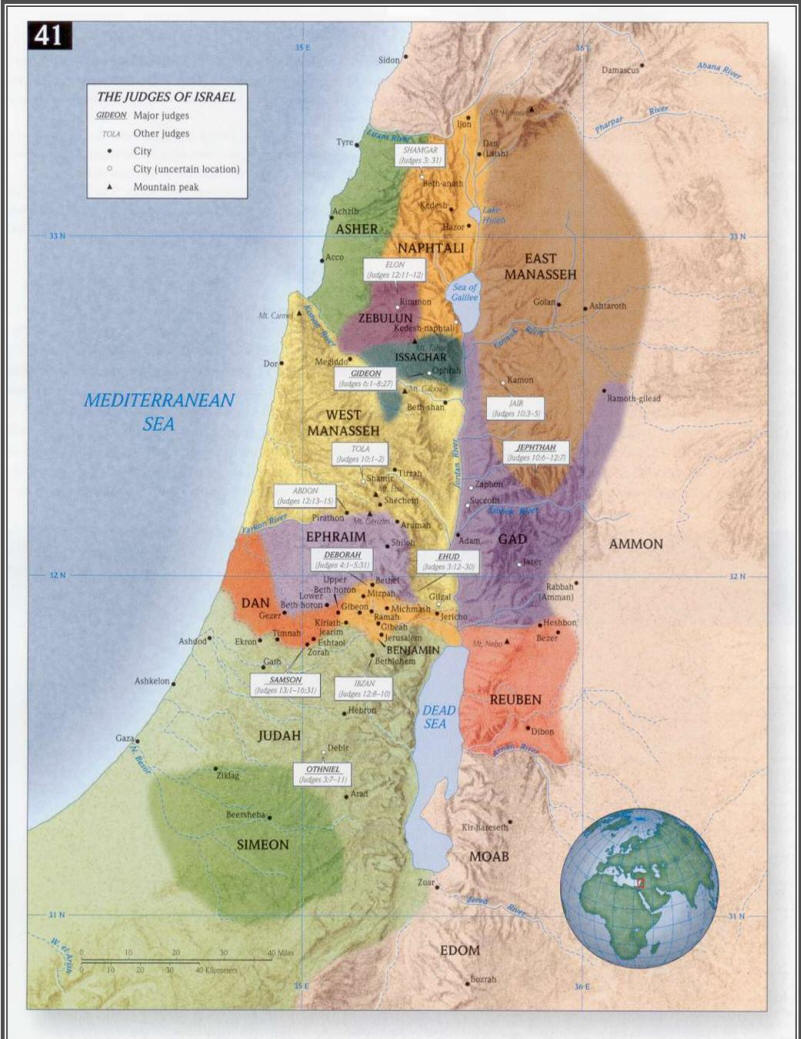
\includegraphics[scale=0.8, angle=0]{07OT-Judges/References/7.Map-Judges}
\caption[Map of the Judges]{Map of the Judges}
\label{fig:Map of the Judges}
\end{center}
\end{figure}


\newpage
\begin{figure}
\begin{center}
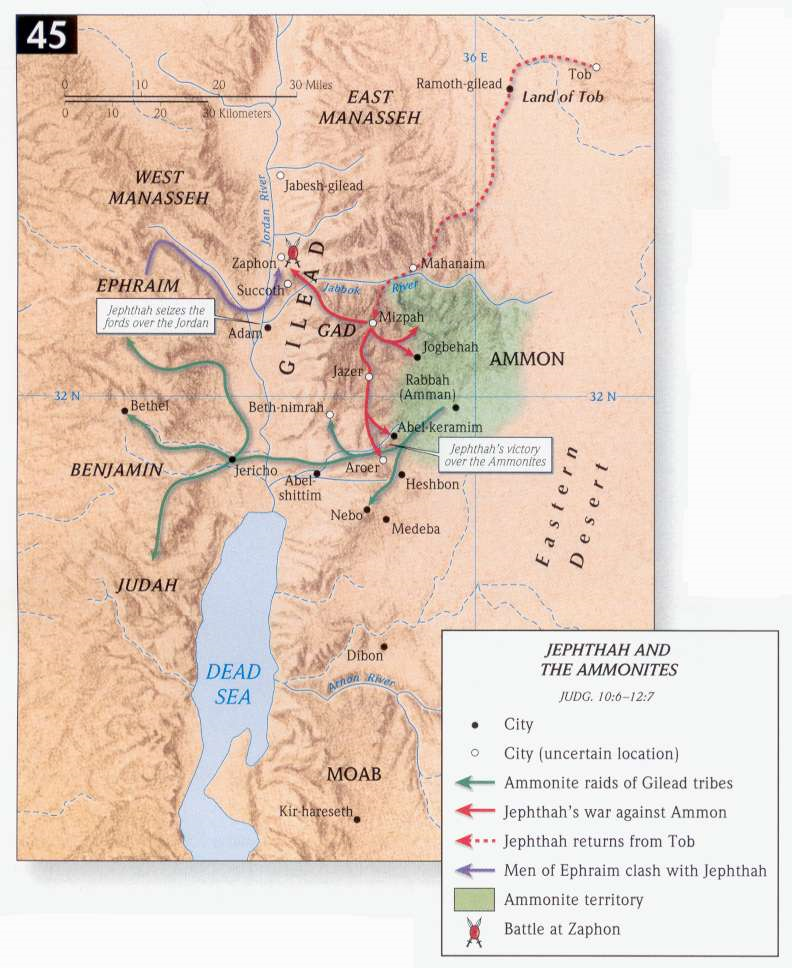
\includegraphics[scale=0.6, angle=0]{07OT-Judges/References/8.Jephthah-Map}
\caption[Map of Jephthah]{Map of Jephthah}
\label{fig:Map of Jephthah}
\end{center}
\end{figure}


\newpage
\begin{figure}
\begin{center}
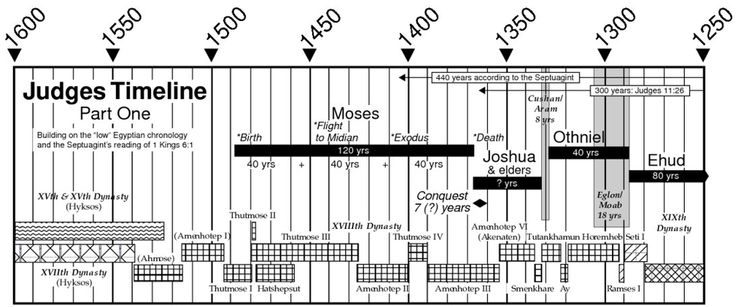
\includegraphics[scale=0.8, angle=90]{07OT-Judges/References/10.Timeline1-Judges}
\caption[Timeline of Judges]{Timeline of Judges}
\label{fig:Timeline of Judges}
\end{center}
\end{figure}



\newpage
\begin{figure}
\begin{center}
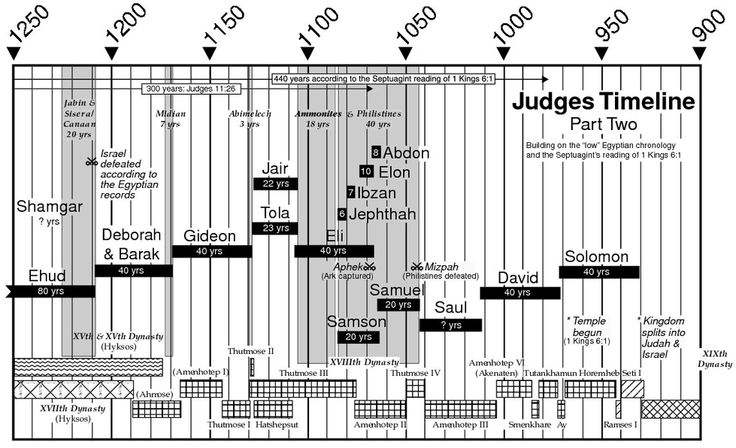
\includegraphics[scale=0.6, angle=90]{07OT-Judges/References/11.Timeline2-Judges}
\caption[Timeline2 of Judges]{Timeline2 of Judges}
\label{fig:Timeline2 of Judges}
\end{center}
\end{figure}


\newpage
\begin{figure}
\begin{center}
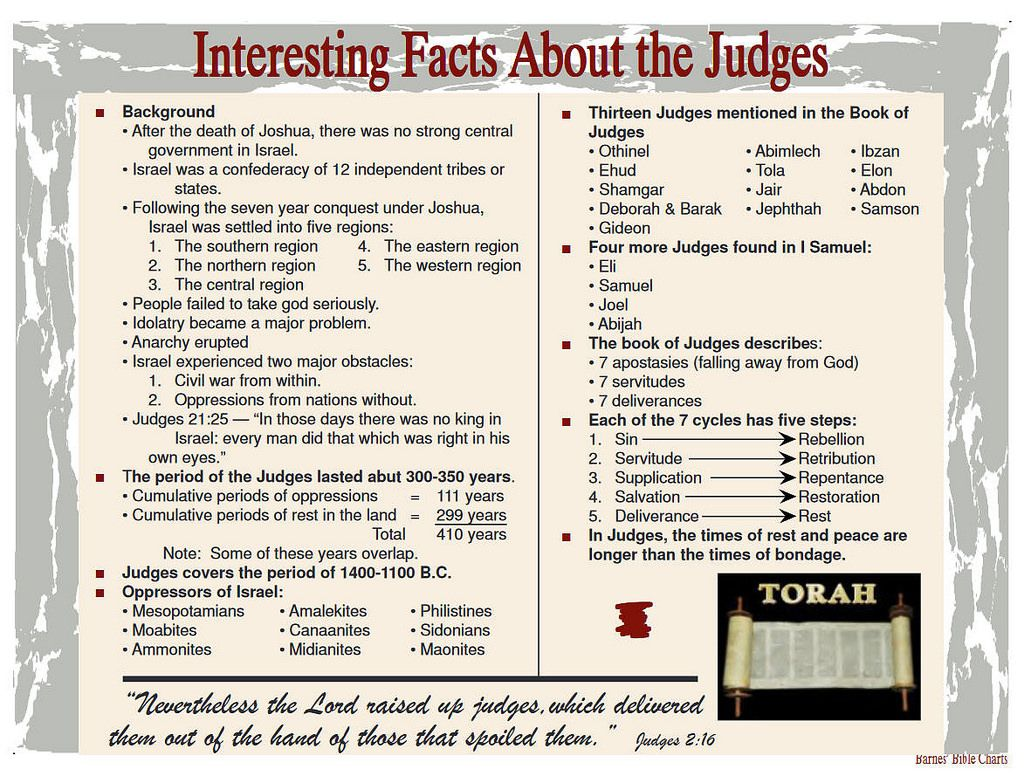
\includegraphics[scale=0.6, angle=90]{07OT-Judges/References/14.InterestingFactsonJudges}
\caption[Interesting Facts about Judges]{Interesting Facts about Judges}
\label{fig:Interesting Facts about Judges}
\end{center}
\end{figure}



\chapter{Judges 10}
 %  \textcolor[cmyk]{0.99998,1,0,0}{

\marginpar{\scriptsize \centering \fcolorbox{black}{lime}{\textbf{2$^{nd}$} WAVE OF JUDGES}\\ (Judges 10) \begin{compactenum}[I.][8]
    \item  \textbf{Declining Character} \index[scripture]{Judges!Jdg 10:04}(Jdg 10:4) -- Tola and Jair are famous for wealth, Jephthah and Samson for their failures
    \item  \textbf{Desperate Conditions} \index[scripture]{Judges!Jdg 10:08}(Jdg 10:8)
    \item  \textbf{Despicable Conduct} \index[scripture]{Judges!Jdg 10:06}(Jdg 10:6)
    \item  A \textbf{Dash of Conscience} \index[scripture]{Judges!Jdg 10:15}(Jdg 10:15)
    \item  A \textbf{Deliverance Cry} \index[scripture]{Judges!Jdg 10:15}(Jdg 10:15)
    \item   \textbf{Dismissed Charges} \index[scripture]{Judges!Jdg 10:16}(Jdg 10:16)
    \item  A \textbf{Desired Champion} \index[scripture]{Judges!Jdg 10:18}(Jdg 10:18)
\end{compactenum}}


\footnote{\textcolor[rgb]{0.00,0.25,0.00}{\hyperlink{JudgesTOC}{Return to end of Table of Contents.}}}\footnote{\href{https://audiobible.com/bible/judges_10.html}{\textcolor[cmyk]{0.99998,1,0,0}{Judges 10 Audio}}}\textcolor[cmyk]{0.99998,1,0,0}{And after Abimelech there arose to defend \fcolorbox{bone}{bone}{Israel} Tola the son of Puah, the son of Dodo, a man of Issachar; and he dwelt in Shamir in mount Ephraim.}
[2] \textcolor[cmyk]{0.99998,1,0,0}{And he judged \fcolorbox{bone}{bone}{Israel} twenty and three years, and died, and was buried in Shamir.}\\
\\
\P \textcolor[cmyk]{0.99998,1,0,0}{And after him arose Jair, a Gileadite, and judged \fcolorbox{bone}{bone}{Israel} twenty and two years.}
[4] \textcolor[cmyk]{0.99998,1,0,0}{And he had thirty sons that rode on thirty ass colts, and they had thirty cities, which are called Havoth-jair unto this day, which \emph{are} in the land of Gilead.}\\
\\
\P \textcolor[cmyk]{0.99998,1,0,0}{And Jair died, and was buried in Camon.}
[6] \textcolor[cmyk]{0.99998,1,0,0}{And \fcolorbox{bone}{bone}{the children of} \fcolorbox{bone}{bone}{Israel} did evil again in the sight of the LORD, and served Baalim, and Ashtaroth, and the gods of Syria, and the gods of Zidon, and the gods of Moab, and the gods of \fcolorbox{bone}{bone}{the children of} Ammon, and the gods of the Philistines, and forsook the LORD, and served not him.}
[7] \textcolor[cmyk]{0.99998,1,0,0}{And the anger of the LORD was hot against \fcolorbox{bone}{bone}{Israel}, and he sold them into the hands of the Philistines, and into the hands of \fcolorbox{bone}{bone}{the children of} Ammon.}
[8] \textcolor[cmyk]{0.99998,1,0,0}{And that year they vexed and oppressed \fcolorbox{bone}{bone}{the children of} \fcolorbox{bone}{bone}{Israel}: eighteen years, all \fcolorbox{bone}{bone}{the children of} \fcolorbox{bone}{bone}{Israel} that \emph{were} on the other side Jordan in the land of the Amorites, which \emph{is} in Gilead.}
[9] \textcolor[cmyk]{0.99998,1,0,0}{Moreover \fcolorbox{bone}{bone}{the children of} Ammon passed over Jordan to fight also against Judah, and against Benjamin, and against the house of Ephraim; so that \fcolorbox{bone}{bone}{Israel} was sore distressed.}\\
\\
\P \textcolor[cmyk]{0.99998,1,0,0}{And \fcolorbox{bone}{bone}{the children of} \fcolorbox{bone}{bone}{Israel} cried unto the LORD, saying, We have sinned against thee, both because we have forsaken our God, and also served Baalim.}
[11] \textcolor[cmyk]{0.99998,1,0,0}{And the LORD said unto \fcolorbox{bone}{bone}{the children of} \fcolorbox{bone}{bone}{Israel}, \emph{Did} not \emph{I} \emph{deliver} \emph{you} from the Egyptians, and from the Amorites, from \fcolorbox{bone}{bone}{the children of} Ammon, and from the Philistines?}
[12] \textcolor[cmyk]{0.99998,1,0,0}{The Zidonians also, and the Amalekites, and the Maonites, did oppress you; and ye cried to me, and I delivered you out of their hand.}
[13] \textcolor[cmyk]{0.99998,1,0,0}{Yet ye have forsaken me, and served other gods: wherefore I will deliver you no more.}
[14] \textcolor[cmyk]{0.99998,1,0,0}{Go and cry unto the gods which ye have chosen; let them deliver you in the time of your tribulation.}\\
\\
\P \textcolor[cmyk]{0.99998,1,0,0}{And \fcolorbox{bone}{bone}{the children of} \fcolorbox{bone}{bone}{Israel} said unto the LORD, We have sinned: do thou unto us whatsoever seemeth good unto thee; deliver us only, we pray thee, this day.}
[16] \textcolor[cmyk]{0.99998,1,0,0}{And they put away the strange gods from among them, and served the LORD: and his soul was grieved for the misery of \fcolorbox{bone}{bone}{Israel}.}
[17] \textcolor[cmyk]{0.99998,1,0,0}{Then \fcolorbox{bone}{bone}{the children of} Ammon were gathered together, and encamped in Gilead. And \fcolorbox{bone}{bone}{the children of} \fcolorbox{bone}{bone}{Israel} assembled themselves together, and encamped in Mizpeh.}
[18] \textcolor[cmyk]{0.99998,1,0,0}{And the people \emph{and} princes of Gilead said one to another, What man \emph{is} \emph{he} that will begin to fight against \fcolorbox{bone}{bone}{the children of} Ammon? he shall be head over all the inhabitants of Gilead.}
\index[NWIV]{29!Judges!Jud 10:1}\index[AWIP]{And!Judges!Jud 10:1}\index[AWIP]{after!Judges!Jud 10:1}\index[AWIP]{Abimelech!Judges!Jud 10:1}\index[AWIP]{there!Judges!Jud 10:1}\index[AWIP]{arose!Judges!Jud 10:1}\index[AWIP]{to!Judges!Jud 10:1}\index[AWIP]{defend!Judges!Jud 10:1}\index[AWIP]{Israel!Judges!Jud 10:1}\index[AWIP]{Tola!Judges!Jud 10:1}\index[AWIP]{the!Judges!Jud 10:1}\index[AWIP]{the!Judges!Jud 10:1 (2)}\index[AWIP]{son!Judges!Jud 10:1}\index[AWIP]{son!Judges!Jud 10:1 (2)}\index[AWIP]{of!Judges!Jud 10:1}\index[AWIP]{of!Judges!Jud 10:1 (2)}\index[AWIP]{of!Judges!Jud 10:1 (3)}\index[AWIP]{Puah!Judges!Jud 10:1}\index[AWIP]{Dodo!Judges!Jud 10:1}\index[AWIP]{a!Judges!Jud 10:1}\index[AWIP]{man!Judges!Jud 10:1}\index[AWIP]{Issachar!Judges!Jud 10:1}\index[AWIP]{and!Judges!Jud 10:1}\index[AWIP]{he!Judges!Jud 10:1}\index[AWIP]{dwelt!Judges!Jud 10:1}\index[AWIP]{in!Judges!Jud 10:1}\index[AWIP]{in!Judges!Jud 10:1 (2)}\index[AWIP]{Shamir!Judges!Jud 10:1}\index[AWIP]{mount!Judges!Jud 10:1}\index[AWIP]{Ephraim!Judges!Jud 10:1}

\index[NWIV]{15!Judges!Jud 10:2}\index[AWIP]{And!Judges!Jud 10:2}\index[AWIP]{he!Judges!Jud 10:2}\index[AWIP]{judged!Judges!Jud 10:2}\index[AWIP]{Israel!Judges!Jud 10:2}\index[AWIP]{twenty!Judges!Jud 10:2}\index[AWIP]{and!Judges!Jud 10:2}\index[AWIP]{and!Judges!Jud 10:2 (2)}\index[AWIP]{and!Judges!Jud 10:2 (3)}\index[AWIP]{three!Judges!Jud 10:2}\index[AWIP]{years!Judges!Jud 10:2}\index[AWIP]{died!Judges!Jud 10:2}\index[AWIP]{was!Judges!Jud 10:2}\index[AWIP]{buried!Judges!Jud 10:2}\index[AWIP]{in!Judges!Jud 10:2}\index[AWIP]{Shamir!Judges!Jud 10:2}

\index[NWIV]{14!Judges!Jud 10:3}\index[AWIP]{And!Judges!Jud 10:3}\index[AWIP]{after!Judges!Jud 10:3}\index[AWIP]{him!Judges!Jud 10:3}\index[AWIP]{arose!Judges!Jud 10:3}\index[AWIP]{Jair!Judges!Jud 10:3}\index[AWIP]{a!Judges!Jud 10:3}\index[AWIP]{Gileadite!Judges!Jud 10:3}\index[AWIP]{and!Judges!Jud 10:3}\index[AWIP]{and!Judges!Jud 10:3 (2)}\index[AWIP]{judged!Judges!Jud 10:3}\index[AWIP]{Israel!Judges!Jud 10:3}\index[AWIP]{twenty!Judges!Jud 10:3}\index[AWIP]{two!Judges!Jud 10:3}\index[AWIP]{years!Judges!Jud 10:3}

\index[NWIV]{30!Judges!Jud 10:4}\index[AWIP]{And!Judges!Jud 10:4}\index[AWIP]{he!Judges!Jud 10:4}\index[AWIP]{had!Judges!Jud 10:4}\index[AWIP]{had!Judges!Jud 10:4 (2)}\index[AWIP]{thirty!Judges!Jud 10:4}\index[AWIP]{thirty!Judges!Jud 10:4 (2)}\index[AWIP]{thirty!Judges!Jud 10:4 (3)}\index[AWIP]{sons!Judges!Jud 10:4}\index[AWIP]{that!Judges!Jud 10:4}\index[AWIP]{rode!Judges!Jud 10:4}\index[AWIP]{on!Judges!Jud 10:4}\index[AWIP]{ass!Judges!Jud 10:4}\index[AWIP]{colts!Judges!Jud 10:4}\index[AWIP]{and!Judges!Jud 10:4}\index[AWIP]{they!Judges!Jud 10:4}\index[AWIP]{cities!Judges!Jud 10:4}\index[AWIP]{which!Judges!Jud 10:4}\index[AWIP]{which!Judges!Jud 10:4 (2)}\index[AWIP]{are!Judges!Jud 10:4}\index[AWIP]{called!Judges!Jud 10:4}\index[AWIP]{Havoth-jair!Judges!Jud 10:4}\index[AWIP]{unto!Judges!Jud 10:4}\index[AWIP]{this!Judges!Jud 10:4}\index[AWIP]{day!Judges!Jud 10:4}\index[AWIP]{\emph{are}!Judges!Jud 10:4}\index[AWIP]{in!Judges!Jud 10:4}\index[AWIP]{the!Judges!Jud 10:4}\index[AWIP]{land!Judges!Jud 10:4}\index[AWIP]{of!Judges!Jud 10:4}\index[AWIP]{Gilead!Judges!Jud 10:4}\index[AWIP]{\emph{are}!Judges!Jud 10:4}

\index[NWIV]{8!Judges!Jud 10:5}\index[AWIP]{And!Judges!Jud 10:5}\index[AWIP]{Jair!Judges!Jud 10:5}\index[AWIP]{died!Judges!Jud 10:5}\index[AWIP]{and!Judges!Jud 10:5}\index[AWIP]{was!Judges!Jud 10:5}\index[AWIP]{buried!Judges!Jud 10:5}\index[AWIP]{in!Judges!Jud 10:5}\index[AWIP]{Camon!Judges!Jud 10:5}

\index[NWIV]{56!Judges!Jud 10:6}\index[AWIP]{And!Judges!Jud 10:6}\index[AWIP]{the!Judges!Jud 10:6}\index[AWIP]{the!Judges!Jud 10:6 (2)}\index[AWIP]{the!Judges!Jud 10:6 (3)}\index[AWIP]{the!Judges!Jud 10:6 (4)}\index[AWIP]{the!Judges!Jud 10:6 (5)}\index[AWIP]{the!Judges!Jud 10:6 (6)}\index[AWIP]{the!Judges!Jud 10:6 (7)}\index[AWIP]{the!Judges!Jud 10:6 (8)}\index[AWIP]{the!Judges!Jud 10:6 (9)}\index[AWIP]{the!Judges!Jud 10:6 (10)}\index[AWIP]{the!Judges!Jud 10:6 (11)}\index[AWIP]{children!Judges!Jud 10:6}\index[AWIP]{children!Judges!Jud 10:6 (2)}\index[AWIP]{of!Judges!Jud 10:6}\index[AWIP]{of!Judges!Jud 10:6 (2)}\index[AWIP]{of!Judges!Jud 10:6 (3)}\index[AWIP]{of!Judges!Jud 10:6 (4)}\index[AWIP]{of!Judges!Jud 10:6 (5)}\index[AWIP]{of!Judges!Jud 10:6 (6)}\index[AWIP]{of!Judges!Jud 10:6 (7)}\index[AWIP]{of!Judges!Jud 10:6 (8)}\index[AWIP]{Israel!Judges!Jud 10:6}\index[AWIP]{did!Judges!Jud 10:6}\index[AWIP]{evil!Judges!Jud 10:6}\index[AWIP]{again!Judges!Jud 10:6}\index[AWIP]{in!Judges!Jud 10:6}\index[AWIP]{sight!Judges!Jud 10:6}\index[AWIP]{LORD!Judges!Jud 10:6}\index[AWIP]{LORD!Judges!Jud 10:6 (2)}\index[AWIP]{and!Judges!Jud 10:6}\index[AWIP]{and!Judges!Jud 10:6 (2)}\index[AWIP]{and!Judges!Jud 10:6 (3)}\index[AWIP]{and!Judges!Jud 10:6 (4)}\index[AWIP]{and!Judges!Jud 10:6 (5)}\index[AWIP]{and!Judges!Jud 10:6 (6)}\index[AWIP]{and!Judges!Jud 10:6 (7)}\index[AWIP]{and!Judges!Jud 10:6 (8)}\index[AWIP]{and!Judges!Jud 10:6 (9)}\index[AWIP]{served!Judges!Jud 10:6}\index[AWIP]{served!Judges!Jud 10:6 (2)}\index[AWIP]{Baalim!Judges!Jud 10:6}\index[AWIP]{Ashtaroth!Judges!Jud 10:6}\index[AWIP]{gods!Judges!Jud 10:6}\index[AWIP]{gods!Judges!Jud 10:6 (2)}\index[AWIP]{gods!Judges!Jud 10:6 (3)}\index[AWIP]{gods!Judges!Jud 10:6 (4)}\index[AWIP]{gods!Judges!Jud 10:6 (5)}\index[AWIP]{Syria!Judges!Jud 10:6}\index[AWIP]{Zidon!Judges!Jud 10:6}\index[AWIP]{Moab!Judges!Jud 10:6}\index[AWIP]{Ammon!Judges!Jud 10:6}\index[AWIP]{Philistines!Judges!Jud 10:6}\index[AWIP]{forsook!Judges!Jud 10:6}\index[AWIP]{not!Judges!Jud 10:6}\index[AWIP]{him!Judges!Jud 10:6}

\index[NWIV]{29!Judges!Jud 10:7}\index[AWIP]{And!Judges!Jud 10:7}\index[AWIP]{the!Judges!Jud 10:7}\index[AWIP]{the!Judges!Jud 10:7 (2)}\index[AWIP]{the!Judges!Jud 10:7 (3)}\index[AWIP]{the!Judges!Jud 10:7 (4)}\index[AWIP]{the!Judges!Jud 10:7 (5)}\index[AWIP]{the!Judges!Jud 10:7 (6)}\index[AWIP]{anger!Judges!Jud 10:7}\index[AWIP]{of!Judges!Jud 10:7}\index[AWIP]{of!Judges!Jud 10:7 (2)}\index[AWIP]{of!Judges!Jud 10:7 (3)}\index[AWIP]{of!Judges!Jud 10:7 (4)}\index[AWIP]{LORD!Judges!Jud 10:7}\index[AWIP]{was!Judges!Jud 10:7}\index[AWIP]{hot!Judges!Jud 10:7}\index[AWIP]{against!Judges!Jud 10:7}\index[AWIP]{Israel!Judges!Jud 10:7}\index[AWIP]{and!Judges!Jud 10:7}\index[AWIP]{and!Judges!Jud 10:7 (2)}\index[AWIP]{he!Judges!Jud 10:7}\index[AWIP]{sold!Judges!Jud 10:7}\index[AWIP]{them!Judges!Jud 10:7}\index[AWIP]{into!Judges!Jud 10:7}\index[AWIP]{into!Judges!Jud 10:7 (2)}\index[AWIP]{hands!Judges!Jud 10:7}\index[AWIP]{hands!Judges!Jud 10:7 (2)}\index[AWIP]{Philistines!Judges!Jud 10:7}\index[AWIP]{children!Judges!Jud 10:7}\index[AWIP]{Ammon!Judges!Jud 10:7}

\index[NWIV]{35!Judges!Jud 10:8}\index[AWIP]{And!Judges!Jud 10:8}\index[AWIP]{that!Judges!Jud 10:8}\index[AWIP]{that!Judges!Jud 10:8 (2)}\index[AWIP]{year!Judges!Jud 10:8}\index[AWIP]{they!Judges!Jud 10:8}\index[AWIP]{vexed!Judges!Jud 10:8}\index[AWIP]{and!Judges!Jud 10:8}\index[AWIP]{oppressed!Judges!Jud 10:8}\index[AWIP]{the!Judges!Jud 10:8}\index[AWIP]{the!Judges!Jud 10:8 (2)}\index[AWIP]{the!Judges!Jud 10:8 (3)}\index[AWIP]{the!Judges!Jud 10:8 (4)}\index[AWIP]{the!Judges!Jud 10:8 (5)}\index[AWIP]{children!Judges!Jud 10:8}\index[AWIP]{children!Judges!Jud 10:8 (2)}\index[AWIP]{of!Judges!Jud 10:8}\index[AWIP]{of!Judges!Jud 10:8 (2)}\index[AWIP]{of!Judges!Jud 10:8 (3)}\index[AWIP]{Israel!Judges!Jud 10:8}\index[AWIP]{Israel!Judges!Jud 10:8 (2)}\index[AWIP]{eighteen!Judges!Jud 10:8}\index[AWIP]{years!Judges!Jud 10:8}\index[AWIP]{all!Judges!Jud 10:8}\index[AWIP]{\emph{were}!Judges!Jud 10:8}\index[AWIP]{on!Judges!Jud 10:8}\index[AWIP]{other!Judges!Jud 10:8}\index[AWIP]{side!Judges!Jud 10:8}\index[AWIP]{Jordan!Judges!Jud 10:8}\index[AWIP]{in!Judges!Jud 10:8}\index[AWIP]{in!Judges!Jud 10:8 (2)}\index[AWIP]{land!Judges!Jud 10:8}\index[AWIP]{Amorites!Judges!Jud 10:8}\index[AWIP]{which!Judges!Jud 10:8}\index[AWIP]{\emph{is}!Judges!Jud 10:8}\index[AWIP]{Gilead!Judges!Jud 10:8}\index[AWIP]{\emph{were}!Judges!Jud 10:8}\index[AWIP]{\emph{is}!Judges!Jud 10:8}

\index[NWIV]{28!Judges!Jud 10:9}\index[AWIP]{Moreover!Judges!Jud 10:9}\index[AWIP]{the!Judges!Jud 10:9}\index[AWIP]{the!Judges!Jud 10:9 (2)}\index[AWIP]{children!Judges!Jud 10:9}\index[AWIP]{of!Judges!Jud 10:9}\index[AWIP]{of!Judges!Jud 10:9 (2)}\index[AWIP]{Ammon!Judges!Jud 10:9}\index[AWIP]{passed!Judges!Jud 10:9}\index[AWIP]{over!Judges!Jud 10:9}\index[AWIP]{Jordan!Judges!Jud 10:9}\index[AWIP]{to!Judges!Jud 10:9}\index[AWIP]{fight!Judges!Jud 10:9}\index[AWIP]{also!Judges!Jud 10:9}\index[AWIP]{against!Judges!Jud 10:9}\index[AWIP]{against!Judges!Jud 10:9 (2)}\index[AWIP]{against!Judges!Jud 10:9 (3)}\index[AWIP]{Judah!Judges!Jud 10:9}\index[AWIP]{and!Judges!Jud 10:9}\index[AWIP]{and!Judges!Jud 10:9 (2)}\index[AWIP]{Benjamin!Judges!Jud 10:9}\index[AWIP]{house!Judges!Jud 10:9}\index[AWIP]{Ephraim!Judges!Jud 10:9}\index[AWIP]{so!Judges!Jud 10:9}\index[AWIP]{that!Judges!Jud 10:9}\index[AWIP]{Israel!Judges!Jud 10:9}\index[AWIP]{was!Judges!Jud 10:9}\index[AWIP]{sore!Judges!Jud 10:9}\index[AWIP]{distressed!Judges!Jud 10:9}

\index[NWIV]{26!Judges!Jud 10:10}\index[AWIP]{And!Judges!Jud 10:10}\index[AWIP]{the!Judges!Jud 10:10}\index[AWIP]{the!Judges!Jud 10:10 (2)}\index[AWIP]{children!Judges!Jud 10:10}\index[AWIP]{of!Judges!Jud 10:10}\index[AWIP]{Israel!Judges!Jud 10:10}\index[AWIP]{cried!Judges!Jud 10:10}\index[AWIP]{unto!Judges!Jud 10:10}\index[AWIP]{LORD!Judges!Jud 10:10}\index[AWIP]{saying!Judges!Jud 10:10}\index[AWIP]{We!Judges!Jud 10:10}\index[AWIP]{have!Judges!Jud 10:10}\index[AWIP]{have!Judges!Jud 10:10 (2)}\index[AWIP]{sinned!Judges!Jud 10:10}\index[AWIP]{against!Judges!Jud 10:10}\index[AWIP]{thee!Judges!Jud 10:10}\index[AWIP]{both!Judges!Jud 10:10}\index[AWIP]{because!Judges!Jud 10:10}\index[AWIP]{we!Judges!Jud 10:10}\index[AWIP]{forsaken!Judges!Jud 10:10}\index[AWIP]{our!Judges!Jud 10:10}\index[AWIP]{God!Judges!Jud 10:10}\index[AWIP]{and!Judges!Jud 10:10}\index[AWIP]{also!Judges!Jud 10:10}\index[AWIP]{served!Judges!Jud 10:10}\index[AWIP]{Baalim!Judges!Jud 10:10}

\index[NWIV]{30!Judges!Jud 10:11}\index[AWIP]{And!Judges!Jud 10:11}\index[AWIP]{the!Judges!Jud 10:11}\index[AWIP]{the!Judges!Jud 10:11 (2)}\index[AWIP]{the!Judges!Jud 10:11 (3)}\index[AWIP]{the!Judges!Jud 10:11 (4)}\index[AWIP]{the!Judges!Jud 10:11 (5)}\index[AWIP]{the!Judges!Jud 10:11 (6)}\index[AWIP]{LORD!Judges!Jud 10:11}\index[AWIP]{said!Judges!Jud 10:11}\index[AWIP]{unto!Judges!Jud 10:11}\index[AWIP]{children!Judges!Jud 10:11}\index[AWIP]{children!Judges!Jud 10:11 (2)}\index[AWIP]{of!Judges!Jud 10:11}\index[AWIP]{of!Judges!Jud 10:11 (2)}\index[AWIP]{Israel!Judges!Jud 10:11}\index[AWIP]{\emph{Did}!Judges!Jud 10:11}\index[AWIP]{not!Judges!Jud 10:11}\index[AWIP]{\emph{I}!Judges!Jud 10:11}\index[AWIP]{\emph{deliver}!Judges!Jud 10:11}\index[AWIP]{\emph{you}!Judges!Jud 10:11}\index[AWIP]{from!Judges!Jud 10:11}\index[AWIP]{from!Judges!Jud 10:11 (2)}\index[AWIP]{from!Judges!Jud 10:11 (3)}\index[AWIP]{from!Judges!Jud 10:11 (4)}\index[AWIP]{Egyptians!Judges!Jud 10:11}\index[AWIP]{and!Judges!Jud 10:11}\index[AWIP]{and!Judges!Jud 10:11 (2)}\index[AWIP]{Amorites!Judges!Jud 10:11}\index[AWIP]{Ammon!Judges!Jud 10:11}\index[AWIP]{Philistines?!Judges!Jud 10:11}\index[AWIP]{\emph{Did}!Judges!Jud 10:11}\index[AWIP]{\emph{I}!Judges!Jud 10:11}\index[AWIP]{\emph{deliver}!Judges!Jud 10:11}\index[AWIP]{\emph{you}!Judges!Jud 10:11}

\index[NWIV]{25!Judges!Jud 10:12}\index[AWIP]{The!Judges!Jud 10:12}\index[AWIP]{Zidonians!Judges!Jud 10:12}\index[AWIP]{also!Judges!Jud 10:12}\index[AWIP]{and!Judges!Jud 10:12}\index[AWIP]{and!Judges!Jud 10:12 (2)}\index[AWIP]{and!Judges!Jud 10:12 (3)}\index[AWIP]{and!Judges!Jud 10:12 (4)}\index[AWIP]{the!Judges!Jud 10:12}\index[AWIP]{the!Judges!Jud 10:12 (2)}\index[AWIP]{Amalekites!Judges!Jud 10:12}\index[AWIP]{Maonites!Judges!Jud 10:12}\index[AWIP]{did!Judges!Jud 10:12}\index[AWIP]{oppress!Judges!Jud 10:12}\index[AWIP]{you!Judges!Jud 10:12}\index[AWIP]{you!Judges!Jud 10:12 (2)}\index[AWIP]{ye!Judges!Jud 10:12}\index[AWIP]{cried!Judges!Jud 10:12}\index[AWIP]{to!Judges!Jud 10:12}\index[AWIP]{me!Judges!Jud 10:12}\index[AWIP]{I!Judges!Jud 10:12}\index[AWIP]{delivered!Judges!Jud 10:12}\index[AWIP]{out!Judges!Jud 10:12}\index[AWIP]{of!Judges!Jud 10:12}\index[AWIP]{their!Judges!Jud 10:12}\index[AWIP]{hand!Judges!Jud 10:12}

\index[NWIV]{16!Judges!Jud 10:13}\index[AWIP]{Yet!Judges!Jud 10:13}\index[AWIP]{ye!Judges!Jud 10:13}\index[AWIP]{have!Judges!Jud 10:13}\index[AWIP]{forsaken!Judges!Jud 10:13}\index[AWIP]{me!Judges!Jud 10:13}\index[AWIP]{and!Judges!Jud 10:13}\index[AWIP]{served!Judges!Jud 10:13}\index[AWIP]{other!Judges!Jud 10:13}\index[AWIP]{gods!Judges!Jud 10:13}\index[AWIP]{wherefore!Judges!Jud 10:13}\index[AWIP]{I!Judges!Jud 10:13}\index[AWIP]{will!Judges!Jud 10:13}\index[AWIP]{deliver!Judges!Jud 10:13}\index[AWIP]{you!Judges!Jud 10:13}\index[AWIP]{no!Judges!Jud 10:13}\index[AWIP]{more!Judges!Jud 10:13}

\index[NWIV]{20!Judges!Jud 10:14}\index[AWIP]{Go!Judges!Jud 10:14}\index[AWIP]{and!Judges!Jud 10:14}\index[AWIP]{cry!Judges!Jud 10:14}\index[AWIP]{unto!Judges!Jud 10:14}\index[AWIP]{the!Judges!Jud 10:14}\index[AWIP]{the!Judges!Jud 10:14 (2)}\index[AWIP]{gods!Judges!Jud 10:14}\index[AWIP]{which!Judges!Jud 10:14}\index[AWIP]{ye!Judges!Jud 10:14}\index[AWIP]{have!Judges!Jud 10:14}\index[AWIP]{chosen!Judges!Jud 10:14}\index[AWIP]{let!Judges!Jud 10:14}\index[AWIP]{them!Judges!Jud 10:14}\index[AWIP]{deliver!Judges!Jud 10:14}\index[AWIP]{you!Judges!Jud 10:14}\index[AWIP]{in!Judges!Jud 10:14}\index[AWIP]{time!Judges!Jud 10:14}\index[AWIP]{of!Judges!Jud 10:14}\index[AWIP]{your!Judges!Jud 10:14}\index[AWIP]{tribulation!Judges!Jud 10:14}

\index[NWIV]{29!Judges!Jud 10:15}\index[AWIP]{And!Judges!Jud 10:15}\index[AWIP]{the!Judges!Jud 10:15}\index[AWIP]{the!Judges!Jud 10:15 (2)}\index[AWIP]{children!Judges!Jud 10:15}\index[AWIP]{of!Judges!Jud 10:15}\index[AWIP]{Israel!Judges!Jud 10:15}\index[AWIP]{said!Judges!Jud 10:15}\index[AWIP]{unto!Judges!Jud 10:15}\index[AWIP]{unto!Judges!Jud 10:15 (2)}\index[AWIP]{unto!Judges!Jud 10:15 (3)}\index[AWIP]{LORD!Judges!Jud 10:15}\index[AWIP]{We!Judges!Jud 10:15}\index[AWIP]{have!Judges!Jud 10:15}\index[AWIP]{sinned!Judges!Jud 10:15}\index[AWIP]{do!Judges!Jud 10:15}\index[AWIP]{thou!Judges!Jud 10:15}\index[AWIP]{us!Judges!Jud 10:15}\index[AWIP]{us!Judges!Jud 10:15 (2)}\index[AWIP]{whatsoever!Judges!Jud 10:15}\index[AWIP]{seemeth!Judges!Jud 10:15}\index[AWIP]{good!Judges!Jud 10:15}\index[AWIP]{thee!Judges!Jud 10:15}\index[AWIP]{thee!Judges!Jud 10:15 (2)}\index[AWIP]{deliver!Judges!Jud 10:15}\index[AWIP]{only!Judges!Jud 10:15}\index[AWIP]{we!Judges!Jud 10:15}\index[AWIP]{pray!Judges!Jud 10:15}\index[AWIP]{this!Judges!Jud 10:15}\index[AWIP]{day!Judges!Jud 10:15}

\index[NWIV]{24!Judges!Jud 10:16}\index[AWIP]{And!Judges!Jud 10:16}\index[AWIP]{they!Judges!Jud 10:16}\index[AWIP]{put!Judges!Jud 10:16}\index[AWIP]{away!Judges!Jud 10:16}\index[AWIP]{the!Judges!Jud 10:16}\index[AWIP]{the!Judges!Jud 10:16 (2)}\index[AWIP]{the!Judges!Jud 10:16 (3)}\index[AWIP]{strange!Judges!Jud 10:16}\index[AWIP]{gods!Judges!Jud 10:16}\index[AWIP]{from!Judges!Jud 10:16}\index[AWIP]{among!Judges!Jud 10:16}\index[AWIP]{them!Judges!Jud 10:16}\index[AWIP]{and!Judges!Jud 10:16}\index[AWIP]{and!Judges!Jud 10:16 (2)}\index[AWIP]{served!Judges!Jud 10:16}\index[AWIP]{LORD!Judges!Jud 10:16}\index[AWIP]{his!Judges!Jud 10:16}\index[AWIP]{soul!Judges!Jud 10:16}\index[AWIP]{was!Judges!Jud 10:16}\index[AWIP]{grieved!Judges!Jud 10:16}\index[AWIP]{for!Judges!Jud 10:16}\index[AWIP]{misery!Judges!Jud 10:16}\index[AWIP]{of!Judges!Jud 10:16}\index[AWIP]{Israel!Judges!Jud 10:16}

\index[NWIV]{24!Judges!Jud 10:17}\index[AWIP]{Then!Judges!Jud 10:17}\index[AWIP]{the!Judges!Jud 10:17}\index[AWIP]{the!Judges!Jud 10:17 (2)}\index[AWIP]{children!Judges!Jud 10:17}\index[AWIP]{children!Judges!Jud 10:17 (2)}\index[AWIP]{of!Judges!Jud 10:17}\index[AWIP]{of!Judges!Jud 10:17 (2)}\index[AWIP]{Ammon!Judges!Jud 10:17}\index[AWIP]{were!Judges!Jud 10:17}\index[AWIP]{gathered!Judges!Jud 10:17}\index[AWIP]{together!Judges!Jud 10:17}\index[AWIP]{together!Judges!Jud 10:17 (2)}\index[AWIP]{and!Judges!Jud 10:17}\index[AWIP]{and!Judges!Jud 10:17 (2)}\index[AWIP]{encamped!Judges!Jud 10:17}\index[AWIP]{encamped!Judges!Jud 10:17 (2)}\index[AWIP]{in!Judges!Jud 10:17}\index[AWIP]{in!Judges!Jud 10:17 (2)}\index[AWIP]{Gilead!Judges!Jud 10:17}\index[AWIP]{And!Judges!Jud 10:17}\index[AWIP]{Israel!Judges!Jud 10:17}\index[AWIP]{assembled!Judges!Jud 10:17}\index[AWIP]{themselves!Judges!Jud 10:17}\index[AWIP]{Mizpeh!Judges!Jud 10:17}

\index[NWIV]{35!Judges!Jud 10:18}\index[AWIP]{And!Judges!Jud 10:18}\index[AWIP]{the!Judges!Jud 10:18}\index[AWIP]{the!Judges!Jud 10:18 (2)}\index[AWIP]{the!Judges!Jud 10:18 (3)}\index[AWIP]{people!Judges!Jud 10:18}\index[AWIP]{\emph{and}!Judges!Jud 10:18}\index[AWIP]{princes!Judges!Jud 10:18}\index[AWIP]{of!Judges!Jud 10:18}\index[AWIP]{of!Judges!Jud 10:18 (2)}\index[AWIP]{of!Judges!Jud 10:18 (3)}\index[AWIP]{Gilead!Judges!Jud 10:18}\index[AWIP]{Gilead!Judges!Jud 10:18 (2)}\index[AWIP]{said!Judges!Jud 10:18}\index[AWIP]{one!Judges!Jud 10:18}\index[AWIP]{to!Judges!Jud 10:18}\index[AWIP]{to!Judges!Jud 10:18 (2)}\index[AWIP]{another!Judges!Jud 10:18}\index[AWIP]{What!Judges!Jud 10:18}\index[AWIP]{man!Judges!Jud 10:18}\index[AWIP]{\emph{is}!Judges!Jud 10:18}\index[AWIP]{\emph{he}!Judges!Jud 10:18}\index[AWIP]{that!Judges!Jud 10:18}\index[AWIP]{will!Judges!Jud 10:18}\index[AWIP]{begin!Judges!Jud 10:18}\index[AWIP]{fight!Judges!Jud 10:18}\index[AWIP]{against!Judges!Jud 10:18}\index[AWIP]{children!Judges!Jud 10:18}\index[AWIP]{Ammon?!Judges!Jud 10:18}\index[AWIP]{he!Judges!Jud 10:18}\index[AWIP]{shall!Judges!Jud 10:18}\index[AWIP]{be!Judges!Jud 10:18}\index[AWIP]{head!Judges!Jud 10:18}\index[AWIP]{over!Judges!Jud 10:18}\index[AWIP]{all!Judges!Jud 10:18}\index[AWIP]{inhabitants!Judges!Jud 10:18}\index[AWIP]{\emph{and}!Judges!Jud 10:18}\index[AWIP]{\emph{is}!Judges!Jud 10:18}\index[AWIP]{\emph{he}!Judges!Jud 10:18}


\section{Judges 10 Outlines}

\subsection{My Outlines}

\subsubsection{2nd Wave of Judges}
\index[speaker]{Keith Anthony!Judges 10 (2nd Wave of Judges)}
\index[series]{Judges (Keith Anthony)!Judges 10 (2nd Wave of Judges)}
\index[date]{2017/03/20!Judges 10 (2nd Wave of Judges) (Keith Anthony)}
%\textbf{Introduction:} Sometimes God's plans do not match our own, or even our understanding. Sometimes it is a matter of just trusting:
\begin{compactenum}[I.][8]
    \item  \textbf{Declining Character} \index[scripture]{Judges!Jdg 10:04}(Jdg 10:4) -- Tola and Jair are famous for wealth, Jephthah and Samson for their failures
    \item  \textbf{Desperate Conditions} \index[scripture]{Judges!Jdg 10:08}(Jdg 10:8)
    \item  \textbf{Despicable Conduct} \index[scripture]{Judges!Jdg 10:06}(Jdg 10:6)
    \item  A \textbf{Dash of Conscience} \index[scripture]{Judges!Jdg 10:15}(Jdg 10:15)
    \item  A \textbf{Deliverance Cry} \index[scripture]{Judges!Jdg 10:15}(Jdg 10:15)
    \item   \textbf{Dismissed Charges} \index[scripture]{Judges!Jdg 10:16}(Jdg 10:16)
    \item  A \textbf{Desired Champion} \index[scripture]{Judges!Jdg 10:18}(Jdg 10:18)
\end{compactenum}


\subsection{Outlines from Others}
\section{Judges 10 Comments}

\subsection{Numeric Nuggets}
\textbf{13: } Verses 2 and 3 have 13 unique words. The words ``Israel'' and ``children'' are used 13 times in the chapter. The phrase ``the children of'' is found 13 times in the chapter.




\subsection{Judges 10 Repeated Phrases}


%%%%%%%%%%
%%%%%%%%%%
\normalsize
 
\begin{center}
\begin{longtable}{|p{3.0in}|p{0.5in}|}
\caption[Judges 10 Repeated Phrases]{Judges 10 Repeated Phrases}\label{table:Repeated Phrases Judges 10} \\
\hline \multicolumn{1}{|c|}{\textbf{Phrase}} & \multicolumn{1}{c|}{\textbf{Frequency}} \\ \hline 
\endfirsthead
 
\multicolumn{2}{c}
{{\bfseries \tablename\ \thetable{} -- continued from previous page}} \\  
\hline \multicolumn{1}{|c|}{\textbf{Phrase}} & \multicolumn{1}{c|}{\textbf{Frequency}} \\ \hline 
\endhead
 
\hline \multicolumn{2}{c}{{ }} \\ \hline
\endfoot 
the children & 13\\ \hline 
the children of & 13\\ \hline 
children of & 13\\ \hline 
of Israel & 8\\ \hline 
And the & 7\\ \hline 
the children of Israel & 7\\ \hline 
children of Israel & 7\\ \hline 
of the & 7\\ \hline 
the LORD & 7\\ \hline 
and the & 7\\ \hline 
the gods & 6\\ \hline 
the children of Ammon & 6\\ \hline 
children of Ammon & 6\\ \hline 
of Ammon & 6\\ \hline 
and the gods & 5\\ \hline 
and the gods of & 5\\ \hline 
the gods of & 5\\ \hline 
gods of & 5\\ \hline 
in the & 4\\ \hline 
And the children & 4\\ \hline 
And the children of & 4\\ \hline 
And the children of Israel & 4\\ \hline 
and served & 4\\ \hline 
unto the & 4\\ \hline 
from the & 4\\ \hline 
of Gilead & 3\\ \hline 
the LORD and & 3\\ \hline 
LORD and & 3\\ \hline 
the Philistines & 3\\ \hline 
\end{longtable}
\end{center}



%%%%%%%%%%
%%%%%%%%%%



\section{Judges 10 Word Statistics}


%%%%%%%%%%
%%%%%%%%%%
\normalsize
 
\begin{center}
\begin{longtable}{l|c|c|c|c}
\caption[Judges 10 Statistics]{Judges 10 Statistics}\label{table:Statistics for Judges 10} \\
\hline \multicolumn{1}{|c|}{\textbf{Verse(s)}} & \multicolumn{1}{|c|}{\textbf{Count}} & \multicolumn{1}{|c|}{\textbf{Unique}} & \multicolumn{1}{|c|}{\textbf{Italics}} & \multicolumn{1}{|c|}{\textbf{Uniq Italic}}  \\ \hline 
\endfirsthead
 
\multicolumn{5}{c}
{{\bfseries \tablename\ \thetable{} -- continued from previous page}} \\  
\hline \multicolumn{1}{|c|}{\textbf{Verse(s)}} & \multicolumn{1}{|c|}{\textbf{Count}} & \multicolumn{1}{|c|}{\textbf{Unique}} & \multicolumn{1}{|c|}{\textbf{Italics}} & \multicolumn{1}{|c|}{\textbf{Uniq Italic}}  \\ \hline 
\endhead
 
\hline \multicolumn{5}{|r|}{{Continued if needed}} \\ \hline
\endfoot 
1 & 29 & 24 & 0 & 0\\ \hline
2 & 15 & 13 & 0 & 0\\ \hline
3 & 14 & 13 & 0 & 0\\ \hline
4 & 30 & 26 & 1 & 1\\ \hline
5 & 8 & 8 & 0 & 0\\ \hline
6 & 56 & 24 & 0 & 0\\ \hline
7 & 29 & 18 & 0 & 0\\ \hline
8 & 35 & 25 & 2 & 2\\ \hline
9 & 28 & 23 & 0 & 0\\ \hline
10 & 26 & 24 & 0 & 0\\ \hline
11 & 30 & 19 & 4 & 4\\ \hline
12 & 25 & 20 & 0 & 0\\ \hline
13 & 16 & 16 & 0 & 0\\ \hline
14 & 20 & 19 & 0 & 0\\ \hline
15 & 29 & 24 & 0 & 0\\ \hline
16 & 24 & 21 & 0 & 0\\ \hline
17 & 24 & 17 & 0 & 0\\ \hline
18 & 35 & 29 & 3 & 3\\ \hline
Total & 473 & 184 & 10 & 9
\end{longtable}
\end{center}



%%%%%%%%%%
%%%%%%%%%%


\subsection{Judges 10 Words by Frequency}


%%%%%%%%%%
%%%%%%%%%%
\normalsize
 
\begin{center}
\begin{longtable}{l|r}
\caption[Judges 10 Words by Frequency]{Judges 10 Words by Frequency}\label{table:WordsbyFrequency for Judges 10} \\
\hline \multicolumn{1}{|c|}{\textbf{Word}} & \multicolumn{1}{c|}{\textbf{Frequency}} \\ \hline 
\endfirsthead
 
\multicolumn{2}{c}
{{\bfseries \tablename\ \thetable{} -- continued from previous page}} \\  
\hline \multicolumn{1}{|c|}{\textbf{Word}} & \multicolumn{1}{c|}{\textbf{Frequency}} \\ \hline 
\endhead
 
\hline \multicolumn{2}{c}{{ }} \\ \hline
\endfoot 
the & 49\\ \hline 
and & 35\\ \hline 
of & 33\\ \hline 
And & 14\\ \hline 
Israel & 13\\ \hline 
children & 13\\ \hline 
in & 11\\ \hline 
gods & 8\\ \hline 
unto & 7\\ \hline 
LORD & 7\\ \hline 
Ammon & 6\\ \hline 
against & 6\\ \hline 
to & 5\\ \hline 
he & 5\\ \hline 
was & 5\\ \hline 
that & 5\\ \hline 
Gilead & 5\\ \hline 
served & 5\\ \hline 
have & 5\\ \hline 
from & 5\\ \hline 
which & 4\\ \hline 
you & 4\\ \hline 
years & 3\\ \hline 
thirty & 3\\ \hline 
they & 3\\ \hline 
Philistines & 3\\ \hline 
them & 3\\ \hline 
also & 3\\ \hline 
thee & 3\\ \hline 
said & 3\\ \hline 
ye & 3\\ \hline 
deliver & 3\\ \hline 
after & 2\\ \hline 
arose & 2\\ \hline 
son & 2\\ \hline 
a & 2\\ \hline 
man & 2\\ \hline 
Shamir & 2\\ \hline 
Ephraim & 2\\ \hline 
judged & 2\\ \hline 
twenty & 2\\ \hline 
died & 2\\ \hline 
buried & 2\\ \hline 
him & 2\\ \hline 
Jair & 2\\ \hline 
had & 2\\ \hline 
on & 2\\ \hline 
this & 2\\ \hline 
day & 2\\ \hline 
land & 2\\ \hline 
did & 2\\ \hline 
Baalim & 2\\ \hline 
not & 2\\ \hline 
into & 2\\ \hline 
hands & 2\\ \hline 
all & 2\\ \hline 
other & 2\\ \hline 
Jordan & 2\\ \hline 
Amorites & 2\\ \hline 
\emph{is} & 2\\ \hline 
over & 2\\ \hline 
fight & 2\\ \hline 
cried & 2\\ \hline 
We & 2\\ \hline 
sinned & 2\\ \hline 
we & 2\\ \hline 
forsaken & 2\\ \hline 
me & 2\\ \hline 
I & 2\\ \hline 
will & 2\\ \hline 
us & 2\\ \hline 
together & 2\\ \hline 
encamped & 2\\ \hline 
Abimelech & 1\\ \hline 
there & 1\\ \hline 
defend & 1\\ \hline 
Tola & 1\\ \hline 
Puah & 1\\ \hline 
Dodo & 1\\ \hline 
Issachar & 1\\ \hline 
dwelt & 1\\ \hline 
mount & 1\\ \hline 
three & 1\\ \hline 
Gileadite & 1\\ \hline 
two & 1\\ \hline 
sons & 1\\ \hline 
rode & 1\\ \hline 
ass & 1\\ \hline 
colts & 1\\ \hline 
cities & 1\\ \hline 
are & 1\\ \hline 
called & 1\\ \hline 
Havoth-jair & 1\\ \hline 
\emph{are} & 1\\ \hline 
Camon & 1\\ \hline 
evil & 1\\ \hline 
again & 1\\ \hline 
sight & 1\\ \hline 
Ashtaroth & 1\\ \hline 
Syria & 1\\ \hline 
Zidon & 1\\ \hline 
Moab & 1\\ \hline 
forsook & 1\\ \hline 
anger & 1\\ \hline 
hot & 1\\ \hline 
sold & 1\\ \hline 
year & 1\\ \hline 
vexed & 1\\ \hline 
oppressed & 1\\ \hline 
eighteen & 1\\ \hline 
\emph{were} & 1\\ \hline 
side & 1\\ \hline 
Moreover & 1\\ \hline 
passed & 1\\ \hline 
Judah & 1\\ \hline 
Benjamin & 1\\ \hline 
house & 1\\ \hline 
so & 1\\ \hline 
sore & 1\\ \hline 
distressed & 1\\ \hline 
saying & 1\\ \hline 
both & 1\\ \hline 
because & 1\\ \hline 
our & 1\\ \hline 
God & 1\\ \hline 
\emph{Did} & 1\\ \hline 
\emph{I} & 1\\ \hline 
\emph{deliver} & 1\\ \hline 
\emph{you} & 1\\ \hline 
Egyptians & 1\\ \hline 
The & 1\\ \hline 
Zidonians & 1\\ \hline 
Amalekites & 1\\ \hline 
Maonites & 1\\ \hline 
oppress & 1\\ \hline 
delivered & 1\\ \hline 
out & 1\\ \hline 
their & 1\\ \hline 
hand & 1\\ \hline 
Yet & 1\\ \hline 
wherefore & 1\\ \hline 
no & 1\\ \hline 
more & 1\\ \hline 
Go & 1\\ \hline 
cry & 1\\ \hline 
chosen & 1\\ \hline 
let & 1\\ \hline 
time & 1\\ \hline 
your & 1\\ \hline 
tribulation & 1\\ \hline 
do & 1\\ \hline 
thou & 1\\ \hline 
whatsoever & 1\\ \hline 
seemeth & 1\\ \hline 
good & 1\\ \hline 
only & 1\\ \hline 
pray & 1\\ \hline 
put & 1\\ \hline 
away & 1\\ \hline 
strange & 1\\ \hline 
among & 1\\ \hline 
his & 1\\ \hline 
soul & 1\\ \hline 
grieved & 1\\ \hline 
for & 1\\ \hline 
misery & 1\\ \hline 
Then & 1\\ \hline 
were & 1\\ \hline 
gathered & 1\\ \hline 
assembled & 1\\ \hline 
themselves & 1\\ \hline 
Mizpeh & 1\\ \hline 
people & 1\\ \hline 
\emph{and} & 1\\ \hline 
princes & 1\\ \hline 
one & 1\\ \hline 
another & 1\\ \hline 
What & 1\\ \hline 
\emph{he} & 1\\ \hline 
begin & 1\\ \hline 
shall & 1\\ \hline 
be & 1\\ \hline 
head & 1\\ \hline 
inhabitants & 1\\ \hline 
\end{longtable}
\end{center}



%%%%%%%%%%
%%%%%%%%%%


\subsection{Judges 10 Words Alphabetically}


%%%%%%%%%%
%%%%%%%%%%
\normalsize
 
\begin{center}
\begin{longtable}{l|r}
\caption[Judges 10 Words Alphabetically]{Judges 10 Words Alphabetically}\label{table:WordsAlphabetically for Judges 10} \\
\hline \multicolumn{1}{|c|}{\textbf{Word}} & \multicolumn{1}{c|}{\textbf{Frequency}} \\ \hline 
\endfirsthead
 
\multicolumn{2}{c}
{{\bfseries \tablename\ \thetable{} -- continued from previous page}} \\  
\hline \multicolumn{1}{|c|}{\textbf{Word}} & \multicolumn{1}{c|}{\textbf{Frequency}} \\ \hline 
\endhead
 
\hline \multicolumn{2}{c}{{ }} \\ \hline
\endfoot 
Abimelech & 1\\ \hline 
Amalekites & 1\\ \hline 
Ammon & 6\\ \hline 
Amorites & 2\\ \hline 
And & 14\\ \hline 
Ashtaroth & 1\\ \hline 
Baalim & 2\\ \hline 
Benjamin & 1\\ \hline 
Camon & 1\\ \hline 
Dodo & 1\\ \hline 
Egyptians & 1\\ \hline 
Ephraim & 2\\ \hline 
Gilead & 5\\ \hline 
Gileadite & 1\\ \hline 
Go & 1\\ \hline 
God & 1\\ \hline 
Havoth-jair & 1\\ \hline 
I & 2\\ \hline 
Israel & 13\\ \hline 
Issachar & 1\\ \hline 
Jair & 2\\ \hline 
Jordan & 2\\ \hline 
Judah & 1\\ \hline 
LORD & 7\\ \hline 
Maonites & 1\\ \hline 
Mizpeh & 1\\ \hline 
Moab & 1\\ \hline 
Moreover & 1\\ \hline 
Philistines & 3\\ \hline 
Puah & 1\\ \hline 
Shamir & 2\\ \hline 
Syria & 1\\ \hline 
The & 1\\ \hline 
Then & 1\\ \hline 
Tola & 1\\ \hline 
We & 2\\ \hline 
What & 1\\ \hline 
Yet & 1\\ \hline 
Zidon & 1\\ \hline 
Zidonians & 1\\ \hline 
\emph{Did} & 1\\ \hline 
\emph{I} & 1\\ \hline 
\emph{and} & 1\\ \hline 
\emph{are} & 1\\ \hline 
\emph{deliver} & 1\\ \hline 
\emph{he} & 1\\ \hline 
\emph{is} & 2\\ \hline 
\emph{were} & 1\\ \hline 
\emph{you} & 1\\ \hline 
a & 2\\ \hline 
after & 2\\ \hline 
again & 1\\ \hline 
against & 6\\ \hline 
all & 2\\ \hline 
also & 3\\ \hline 
among & 1\\ \hline 
and & 35\\ \hline 
anger & 1\\ \hline 
another & 1\\ \hline 
are & 1\\ \hline 
arose & 2\\ \hline 
ass & 1\\ \hline 
assembled & 1\\ \hline 
away & 1\\ \hline 
be & 1\\ \hline 
because & 1\\ \hline 
begin & 1\\ \hline 
both & 1\\ \hline 
buried & 2\\ \hline 
called & 1\\ \hline 
children & 13\\ \hline 
chosen & 1\\ \hline 
cities & 1\\ \hline 
colts & 1\\ \hline 
cried & 2\\ \hline 
cry & 1\\ \hline 
day & 2\\ \hline 
defend & 1\\ \hline 
deliver & 3\\ \hline 
delivered & 1\\ \hline 
did & 2\\ \hline 
died & 2\\ \hline 
distressed & 1\\ \hline 
do & 1\\ \hline 
dwelt & 1\\ \hline 
eighteen & 1\\ \hline 
encamped & 2\\ \hline 
evil & 1\\ \hline 
fight & 2\\ \hline 
for & 1\\ \hline 
forsaken & 2\\ \hline 
forsook & 1\\ \hline 
from & 5\\ \hline 
gathered & 1\\ \hline 
gods & 8\\ \hline 
good & 1\\ \hline 
grieved & 1\\ \hline 
had & 2\\ \hline 
hand & 1\\ \hline 
hands & 2\\ \hline 
have & 5\\ \hline 
he & 5\\ \hline 
head & 1\\ \hline 
him & 2\\ \hline 
his & 1\\ \hline 
hot & 1\\ \hline 
house & 1\\ \hline 
in & 11\\ \hline 
inhabitants & 1\\ \hline 
into & 2\\ \hline 
judged & 2\\ \hline 
land & 2\\ \hline 
let & 1\\ \hline 
man & 2\\ \hline 
me & 2\\ \hline 
misery & 1\\ \hline 
more & 1\\ \hline 
mount & 1\\ \hline 
no & 1\\ \hline 
not & 2\\ \hline 
of & 33\\ \hline 
on & 2\\ \hline 
one & 1\\ \hline 
only & 1\\ \hline 
oppress & 1\\ \hline 
oppressed & 1\\ \hline 
other & 2\\ \hline 
our & 1\\ \hline 
out & 1\\ \hline 
over & 2\\ \hline 
passed & 1\\ \hline 
people & 1\\ \hline 
pray & 1\\ \hline 
princes & 1\\ \hline 
put & 1\\ \hline 
rode & 1\\ \hline 
said & 3\\ \hline 
saying & 1\\ \hline 
seemeth & 1\\ \hline 
served & 5\\ \hline 
shall & 1\\ \hline 
side & 1\\ \hline 
sight & 1\\ \hline 
sinned & 2\\ \hline 
so & 1\\ \hline 
sold & 1\\ \hline 
son & 2\\ \hline 
sons & 1\\ \hline 
sore & 1\\ \hline 
soul & 1\\ \hline 
strange & 1\\ \hline 
that & 5\\ \hline 
the & 49\\ \hline 
thee & 3\\ \hline 
their & 1\\ \hline 
them & 3\\ \hline 
themselves & 1\\ \hline 
there & 1\\ \hline 
they & 3\\ \hline 
thirty & 3\\ \hline 
this & 2\\ \hline 
thou & 1\\ \hline 
three & 1\\ \hline 
time & 1\\ \hline 
to & 5\\ \hline 
together & 2\\ \hline 
tribulation & 1\\ \hline 
twenty & 2\\ \hline 
two & 1\\ \hline 
unto & 7\\ \hline 
us & 2\\ \hline 
vexed & 1\\ \hline 
was & 5\\ \hline 
we & 2\\ \hline 
were & 1\\ \hline 
whatsoever & 1\\ \hline 
wherefore & 1\\ \hline 
which & 4\\ \hline 
will & 2\\ \hline 
ye & 3\\ \hline 
year & 1\\ \hline 
years & 3\\ \hline 
you & 4\\ \hline 
your & 1\\ \hline 
\end{longtable}
\end{center}



%%%%%%%%%%
%%%%%%%%%%


\subsection{Judges 10 Words by Length}


%%%%%%%%%%
%%%%%%%%%%
\normalsize
 
\begin{center}
\begin{longtable}{l|p{3.75in}}
\caption[Judges 10 Words by Length]{Judges 10 Words by Length}\label{table:WordsAlphabetically for Judges 10} \\
\hline \multicolumn{1}{|c|}{\textbf{Length}} & \multicolumn{1}{c|}{\textbf{Words}} \\ \hline 
\endfirsthead
\hline \multicolumn{1}{|c|}{\textbf{Length}} & \multicolumn{1}{c|}{\textbf{Words}} \\ \hline 
\multicolumn{2}{c}
{{\bfseries \tablename\ \thetable{} -- continued from previous page}} \\  
\hline \multicolumn{1}{|c|}{\textbf{Word}} & \multicolumn{1}{c|}{\textbf{Frequency}} \\ \hline 
\endhead
 
\hline \multicolumn{2}{c}{{ }} \\ \hline
\endfoot 
1 & a, \emph{I}, I\\ \hline 
2 & to, of, he, in, on, \emph{is}, so, We, we, ye, me, no, Go, do, us, \emph{he}, be\\ \hline 
3 & And, the, son, man, and, was, him, two, had, ass, are, day, \emph{are}, did, not, hot, all, our, God, \emph{Did}, \emph{you}, The, you, out, Yet, cry, let, put, his, for, \emph{and}, one\\ \hline 
4 & Tola, Puah, Dodo, died, Jair, sons, that, rode, they, unto, this, land, evil, LORD, gods, Moab, sold, them, into, year, \emph{were}, side, over, also, sore, have, thee, both, said, from, hand, will, more, time, your, thou, good, only, pray, away, soul, Then, were, What, head\\ \hline 
5 & after, there, arose, dwelt, mount, three, years, colts, which, Camon, again, sight, Syria, Zidon, Ammon, anger, hands, vexed, other, fight, Judah, house, cried, their, among, begin, shall\\ \hline 
6 & defend, Israel, Shamir, judged, twenty, buried, thirty, cities, called, Gilead, served, Baalim, Jordan, passed, saying, sinned, chosen, misery, Mizpeh, people\\ \hline 
7 & Ephraim, forsook, against, because, \emph{deliver}, oppress, deliver, seemeth, strange, grieved, princes, another\\ \hline 
8 & Issachar, children, eighteen, Amorites, Moreover, Benjamin, forsaken, Maonites, gathered, together, encamped\\ \hline 
9 & Abimelech, Gileadite, Ashtaroth, oppressed, Egyptians, Zidonians, delivered, wherefore, assembled\\ \hline 
10 & distressed, Amalekites, whatsoever, themselves\\ \hline 
11 & Havoth-jair, Philistines, tribulation, inhabitants\\ \hline 
\end{longtable}
\end{center}



%%%%%%%%%%
%%%%%%%%%%




\chapter{Judges 11}
 %  \textcolor[cmyk]{0.99998,1,0,0}{

\marginpar{\scriptsize \centering \fcolorbox{bone}{lime}{CHOOSING JEPHTHAH}\\ (Judges 11) \begin{compactenum}[I.][8]
    \item  The \textbf{Rejection} \index[scripture]{Judges!Jdg 11:01}(Jdg 11:2) 
    \item  A \textbf{Reputation} \index[scripture]{Judges!Jdg 11:06}(Jdg 11:6) 
    \item  The \textbf{Request} \index[scripture]{Judges!Jdg 11:09}(Jdg 11:9) 
    \item  A Heathen \textbf{Ritual} \index[scripture]{Judges!Jdg 11:31}(Jdg 11:31) 
    \item  The \textbf{Return} \index[scripture]{Judges!Jdg 11:34}(Jdg 11:34) 
    \item  The \textbf{Rending} \index[scripture]{Judges!Jdg 11:35}(Jdg 11:35) 
    \item  The \textbf{Remembrance} \index[scripture]{Judges!Jdg 11:40}(Jdg 11:40) 
\end{compactenum}}

\marginpar{\scriptsize \centering \fcolorbox{bone}{yellow}{JEPHTHAH'S VOW}\\ (Judges 11) \begin{compactenum}[I.][8]
    \item  The \textbf{Rash Vow} \index[scripture]{Judges!Jdg 11:31}(Jdg 11:31) 
    \item  The \textbf{Rash Vow} \index[scripture]{Judges!Jdg 11:31}(Jdg 11:31) 
    \item  A \textbf{Religious Vision} \index[scripture]{Judges!Jdg 11:34}(Jdg 11:34) 
    \item  The \textbf{Rent Clother} \index[scripture]{Judges!Jdg 11:35}(Jdg 11:35) 
    \item  \textbf{Regrest \& Revenge} \index[scripture]{Judges!Jdg 112}(Jdg 112) 
\end{compactenum}}


\footnote{\textcolor[rgb]{0.00,0.25,0.00}{\hyperlink{JudgesTOC}{Return to end of Table of Contents.}}}\footnote{\href{https://audiobible.com/bible/judges_11.html}{\textcolor[cmyk]{0.99998,1,0,0}{Judges 11 Audio}}}\textcolor[cmyk]{0.99998,1,0,0}{Now Jephthah the Gileadite was a mighty man of valour, and he \emph{was} the son of an harlot: and Gilead begat Jephthah.}
[2] \textcolor[cmyk]{0.99998,1,0,0}{And Gilead's wife bare him sons; and his wife's sons grew up, and they thrust out Jephthah, and \fcolorbox{bone}{bone}{said} unto him, Thou shalt not inherit in our father's house; for thou \emph{art} the son of a strange woman.}
[3] \textcolor[cmyk]{0.99998,1,0,0}{Then Jephthah fled from his brethren, and dwelt in the land of Tob: and there were gathered vain men to Jephthah, and went out with him.}\\
\\
\P \textcolor[cmyk]{0.99998,1,0,0}{And it came to pass in process of time, that the children of Ammon made war against Israel.}
[5] \textcolor[cmyk]{0.99998,1,0,0}{And it was so, that when the children of Ammon made war against Israel, the elders of Gilead went to fetch Jephthah out of the land of Tob:}
[6] \textcolor[cmyk]{0.99998,1,0,0}{And they \fcolorbox{bone}{bone}{said} unto Jephthah, Come, and be our captain, that we may fight with the children of Ammon.}
[7] \textcolor[cmyk]{0.99998,1,0,0}{And Jephthah \fcolorbox{bone}{bone}{said} unto the elders of Gilead, Did not ye hate me, and expel me out of my father's house? and why are ye come unto me now when ye are in distress?}
[8] \textcolor[cmyk]{0.99998,1,0,0}{And the elders of Gilead \fcolorbox{bone}{bone}{said} unto Jephthah, Therefore we turn again to thee now, that thou mayest go with us, and fight against the children of Ammon, and be our head over all the inhabitants of Gilead.}
[9] \textcolor[cmyk]{0.99998,1,0,0}{And Jephthah \fcolorbox{bone}{bone}{said} unto the elders of Gilead, If ye bring me home again to fight against the children of Ammon, and the \fcolorbox{bone}{bone}{LORD} deliver them before me, shall I be your head?}
[10] \textcolor[cmyk]{0.99998,1,0,0}{And the elders of Gilead \fcolorbox{bone}{bone}{said} unto Jephthah, The \fcolorbox{bone}{bone}{LORD} be witness between us, if we do not so according to thy words.}
[11] \textcolor[cmyk]{0.99998,1,0,0}{Then Jephthah went with the elders of Gilead, and the people made him head and captain over them: and Jephthah uttered all his words before the \fcolorbox{bone}{bone}{LORD} in Mizpeh.}\\
\\
\P \textcolor[cmyk]{0.99998,1,0,0}{And Jephthah sent messengers unto the king of the children of Ammon, saying, What hast thou to do with me, that thou art come against me to fight in my land?}
[13] \textcolor[cmyk]{0.99998,1,0,0}{And the king of the children of Ammon answered unto the messengers of Jephthah, Because Israel took away my land, when they came up out of Egypt, from Arnon even unto Jabbok, and unto Jordan: now therefore restore those \emph{lands} again peaceably.}
[14] \textcolor[cmyk]{0.99998,1,0,0}{And Jephthah sent messengers again unto the king of the children of Ammon:}
[15] \textcolor[cmyk]{0.99998,1,0,0}{And \fcolorbox{bone}{bone}{said} unto him, Thus saith Jephthah, Israel took not away the land of Moab, nor the land of the children of Ammon:}
[16] \textcolor[cmyk]{0.99998,1,0,0}{But when Israel came up from Egypt, and walked through the wilderness unto the Red sea, and came to Kadesh;}\
[17] \textcolor[cmyk]{0.99998,1,0,0}{Then Israel sent messengers unto the king of Edom, saying, Let me, I pray thee, pass through thy land: but the king of Edom would not hearken \emph{thereto}. And in like manner they sent unto the king of Moab: but he would not \emph{consent}: and Israel abode in Kadesh.}
[18] \textcolor[cmyk]{0.99998,1,0,0}{Then they went along through the wilderness, and compassed the land of Edom, and the land of Moab, and came by the east side of the land of Moab, and pitched on the other side of Arnon, but came not within the border of Moab: for Arnon \emph{was} the border of Moab.}
[19] \textcolor[cmyk]{0.99998,1,0,0}{And Israel sent messengers unto Sihon king of the Amorites, the king of Heshbon; and Israel \fcolorbox{bone}{bone}{said} unto him, Let us pass, we pray thee, through thy land into my place.}
[20] \textcolor[cmyk]{0.99998,1,0,0}{But Sihon trusted not Israel to pass through his coast: but Sihon gathered all his people together, and pitched in Jahaz, and fought against Israel.}
[21] \textcolor[cmyk]{0.99998,1,0,0}{And the \fcolorbox{bone}{bone}{LORD} God of Israel delivered Sihon and all his people into the hand of Israel, and they smote them: so Israel possessed all the land of the Amorites, the inhabitants of that country.}
[22] \textcolor[cmyk]{0.99998,1,0,0}{And they possessed all the coasts of the Amorites, from Arnon even unto Jabbok, and from the wilderness even unto Jordan.}
[23] \textcolor[cmyk]{0.99998,1,0,0}{So now the \fcolorbox{bone}{bone}{LORD} God of Israel hath dispossessed the Amorites from before his people Israel, and shouldest thou possess it?}
[24] \textcolor[cmyk]{0.99998,1,0,0}{Wilt not thou possess that which Chemosh thy god giveth thee to possess? So whomsoever the \fcolorbox{bone}{bone}{LORD} our God shall drive out from before us, them will we possess.}
[25] \textcolor[cmyk]{0.99998,1,0,0}{And now \emph{art} thou any thing better than Balak the son of Zippor, king of Moab? did he ever strive against Israel, or did he ever fight against them,}
[26] \textcolor[cmyk]{0.99998,1,0,0}{While Israel dwelt in Heshbon and her towns, and in Aroer and her towns, and in all the cities that \emph{be} along by the coasts of Arnon, three hundred years? why therefore did ye not recover \emph{them} within that time?}
[27] \textcolor[cmyk]{0.99998,1,0,0}{Wherefore I have not sinned against thee, but thou doest me wrong to war against me: the \fcolorbox{bone}{bone}{LORD} the Judge be judge this day between the children of Israel and the children of Ammon.}
[28] \textcolor[cmyk]{0.99998,1,0,0}{Howbeit the king of the children of Ammon hearkened not unto the words of Jephthah which he sent him.}\\
\\
\P \textcolor[cmyk]{0.99998,1,0,0}{Then the Spirit of the \fcolorbox{bone}{bone}{LORD} came upon Jephthah, and he passed over Gilead, and Manasseh, and passed over Mizpeh of Gilead, and from Mizpeh of Gilead he passed over \emph{unto} the children of Ammon.}
[30] \textcolor[cmyk]{0.99998,1,0,0}{And Jephthah vowed a vow unto the \fcolorbox{bone}{bone}{LORD}, and \fcolorbox{bone}{bone}{said}, If thou shalt without fail deliver the children of Ammon into mine hands,}
[31] \textcolor[cmyk]{0.99998,1,0,0}{Then it shall be, that whatsoever cometh forth of the doors of my house to meet me, when I return in peace from the children of Ammon, shall surely be the LORD'S, and I will offer it up for a burnt offering.}\\
\\
\P \textcolor[cmyk]{0.99998,1,0,0}{So Jephthah passed over unto the children of Ammon to fight against them; and the \fcolorbox{bone}{bone}{LORD} delivered them into his hands.}
[33] \textcolor[cmyk]{0.99998,1,0,0}{And he smote them from Aroer, even till thou come to Minnith, \emph{even} twenty cities, and unto the plain of the vineyards, with a very great slaughter. Thus the children of Ammon were subdued before the children of Israel.}\\
\\
\P \textcolor[cmyk]{0.99998,1,0,0}{And Jephthah came to Mizpeh unto his house, and, behold, his daughter came out to meet him with timbrels and with dances: and she \emph{was} \emph{his} only child; beside her he had neither son nor daughter.}
[35] \textcolor[cmyk]{0.99998,1,0,0}{And it came to pass, when he saw her, that he rent his clothes, and \fcolorbox{bone}{bone}{said}, Alas, my daughter! thou hast brought me very low, and thou art one of them that trouble me: for I have opened my mouth unto the \fcolorbox{bone}{bone}{LORD}, and I cannot go back.}
[36] \textcolor[cmyk]{0.99998,1,0,0}{And she \fcolorbox{bone}{bone}{said} unto him, My father, \emph{if} thou hast opened thy mouth unto the \fcolorbox{bone}{bone}{LORD}, do to me according to that which hath proceeded out of thy mouth; forasmuch as the \fcolorbox{bone}{bone}{LORD} hath taken vengeance for thee of thine enemies, \emph{even} of the children of Ammon.}
[37] \textcolor[cmyk]{0.99998,1,0,0}{And she \fcolorbox{bone}{bone}{said} unto her father, Let this thing be done for me: let me alone two months, that I may go up and down upon the mountains, and bewail my virginity, I and my fellows.}
[38] \textcolor[cmyk]{0.99998,1,0,0}{And he \fcolorbox{bone}{bone}{said}, Go. And he sent her away \emph{for} two months: and she went with her companions, and bewailed her virginity upon the mountains.}
[39] \textcolor[cmyk]{0.99998,1,0,0}{And it came to pass at the end of two months, that she returned unto her father, who did with her \emph{according} to his vow which he had vowed: and she knew no man. And it was a custom in Israel,}
[40] \textcolor[cmyk]{0.99998,1,0,0}{\emph{That} the daughters of Israel went yearly to lament the daughter of Jephthah the Gileadite four days in a year.}
\index[NWIV]{22!Judges!Jud 11:1}\index[AWIP]{Now!Judges!Jud 11:1}\index[AWIP]{Jephthah!Judges!Jud 11:1}\index[AWIP]{Jephthah!Judges!Jud 11:1 (2)}\index[AWIP]{the!Judges!Jud 11:1}\index[AWIP]{the!Judges!Jud 11:1 (2)}\index[AWIP]{Gileadite!Judges!Jud 11:1}\index[AWIP]{was!Judges!Jud 11:1}\index[AWIP]{a!Judges!Jud 11:1}\index[AWIP]{mighty!Judges!Jud 11:1}\index[AWIP]{man!Judges!Jud 11:1}\index[AWIP]{of!Judges!Jud 11:1}\index[AWIP]{of!Judges!Jud 11:1 (2)}\index[AWIP]{valour!Judges!Jud 11:1}\index[AWIP]{and!Judges!Jud 11:1}\index[AWIP]{and!Judges!Jud 11:1 (2)}\index[AWIP]{he!Judges!Jud 11:1}\index[AWIP]{\emph{was}!Judges!Jud 11:1}\index[AWIP]{son!Judges!Jud 11:1}\index[AWIP]{an!Judges!Jud 11:1}\index[AWIP]{harlot!Judges!Jud 11:1}\index[AWIP]{Gilead!Judges!Jud 11:1}\index[AWIP]{begat!Judges!Jud 11:1}\index[AWIP]{\emph{was}!Judges!Jud 11:1}

\index[NWIV]{38!Judges!Jud 11:2}\index[AWIP]{And!Judges!Jud 11:2}\index[AWIP]{Gilead's!Judges!Jud 11:2}\index[AWIP]{wife!Judges!Jud 11:2}\index[AWIP]{bare!Judges!Jud 11:2}\index[AWIP]{him!Judges!Jud 11:2}\index[AWIP]{him!Judges!Jud 11:2 (2)}\index[AWIP]{sons!Judges!Jud 11:2}\index[AWIP]{sons!Judges!Jud 11:2 (2)}\index[AWIP]{and!Judges!Jud 11:2}\index[AWIP]{and!Judges!Jud 11:2 (2)}\index[AWIP]{and!Judges!Jud 11:2 (3)}\index[AWIP]{his!Judges!Jud 11:2}\index[AWIP]{wife's!Judges!Jud 11:2}\index[AWIP]{grew!Judges!Jud 11:2}\index[AWIP]{up!Judges!Jud 11:2}\index[AWIP]{they!Judges!Jud 11:2}\index[AWIP]{thrust!Judges!Jud 11:2}\index[AWIP]{out!Judges!Jud 11:2}\index[AWIP]{Jephthah!Judges!Jud 11:2}\index[AWIP]{said!Judges!Jud 11:2}\index[AWIP]{unto!Judges!Jud 11:2}\index[AWIP]{Thou!Judges!Jud 11:2}\index[AWIP]{shalt!Judges!Jud 11:2}\index[AWIP]{not!Judges!Jud 11:2}\index[AWIP]{inherit!Judges!Jud 11:2}\index[AWIP]{in!Judges!Jud 11:2}\index[AWIP]{our!Judges!Jud 11:2}\index[AWIP]{father's!Judges!Jud 11:2}\index[AWIP]{house!Judges!Jud 11:2}\index[AWIP]{for!Judges!Jud 11:2}\index[AWIP]{thou!Judges!Jud 11:2}\index[AWIP]{\emph{art}!Judges!Jud 11:2}\index[AWIP]{the!Judges!Jud 11:2}\index[AWIP]{son!Judges!Jud 11:2}\index[AWIP]{of!Judges!Jud 11:2}\index[AWIP]{a!Judges!Jud 11:2}\index[AWIP]{strange!Judges!Jud 11:2}\index[AWIP]{woman!Judges!Jud 11:2}\index[AWIP]{\emph{art}!Judges!Jud 11:2}

\index[NWIV]{26!Judges!Jud 11:3}\index[AWIP]{Then!Judges!Jud 11:3}\index[AWIP]{Jephthah!Judges!Jud 11:3}\index[AWIP]{Jephthah!Judges!Jud 11:3 (2)}\index[AWIP]{fled!Judges!Jud 11:3}\index[AWIP]{from!Judges!Jud 11:3}\index[AWIP]{his!Judges!Jud 11:3}\index[AWIP]{brethren!Judges!Jud 11:3}\index[AWIP]{and!Judges!Jud 11:3}\index[AWIP]{and!Judges!Jud 11:3 (2)}\index[AWIP]{and!Judges!Jud 11:3 (3)}\index[AWIP]{dwelt!Judges!Jud 11:3}\index[AWIP]{in!Judges!Jud 11:3}\index[AWIP]{the!Judges!Jud 11:3}\index[AWIP]{land!Judges!Jud 11:3}\index[AWIP]{of!Judges!Jud 11:3}\index[AWIP]{Tob!Judges!Jud 11:3}\index[AWIP]{there!Judges!Jud 11:3}\index[AWIP]{were!Judges!Jud 11:3}\index[AWIP]{gathered!Judges!Jud 11:3}\index[AWIP]{vain!Judges!Jud 11:3}\index[AWIP]{men!Judges!Jud 11:3}\index[AWIP]{to!Judges!Jud 11:3}\index[AWIP]{went!Judges!Jud 11:3}\index[AWIP]{out!Judges!Jud 11:3}\index[AWIP]{with!Judges!Jud 11:3}\index[AWIP]{him!Judges!Jud 11:3}

\index[NWIV]{18!Judges!Jud 11:4}\index[AWIP]{And!Judges!Jud 11:4}\index[AWIP]{it!Judges!Jud 11:4}\index[AWIP]{came!Judges!Jud 11:4}\index[AWIP]{to!Judges!Jud 11:4}\index[AWIP]{pass!Judges!Jud 11:4}\index[AWIP]{in!Judges!Jud 11:4}\index[AWIP]{process!Judges!Jud 11:4}\index[AWIP]{of!Judges!Jud 11:4}\index[AWIP]{of!Judges!Jud 11:4 (2)}\index[AWIP]{time!Judges!Jud 11:4}\index[AWIP]{that!Judges!Jud 11:4}\index[AWIP]{the!Judges!Jud 11:4}\index[AWIP]{children!Judges!Jud 11:4}\index[AWIP]{Ammon!Judges!Jud 11:4}\index[AWIP]{made!Judges!Jud 11:4}\index[AWIP]{war!Judges!Jud 11:4}\index[AWIP]{against!Judges!Jud 11:4}\index[AWIP]{Israel!Judges!Jud 11:4}

\index[NWIV]{28!Judges!Jud 11:5}\index[AWIP]{And!Judges!Jud 11:5}\index[AWIP]{it!Judges!Jud 11:5}\index[AWIP]{was!Judges!Jud 11:5}\index[AWIP]{so!Judges!Jud 11:5}\index[AWIP]{that!Judges!Jud 11:5}\index[AWIP]{when!Judges!Jud 11:5}\index[AWIP]{the!Judges!Jud 11:5}\index[AWIP]{the!Judges!Jud 11:5 (2)}\index[AWIP]{the!Judges!Jud 11:5 (3)}\index[AWIP]{children!Judges!Jud 11:5}\index[AWIP]{of!Judges!Jud 11:5}\index[AWIP]{of!Judges!Jud 11:5 (2)}\index[AWIP]{of!Judges!Jud 11:5 (3)}\index[AWIP]{of!Judges!Jud 11:5 (4)}\index[AWIP]{Ammon!Judges!Jud 11:5}\index[AWIP]{made!Judges!Jud 11:5}\index[AWIP]{war!Judges!Jud 11:5}\index[AWIP]{against!Judges!Jud 11:5}\index[AWIP]{Israel!Judges!Jud 11:5}\index[AWIP]{elders!Judges!Jud 11:5}\index[AWIP]{Gilead!Judges!Jud 11:5}\index[AWIP]{went!Judges!Jud 11:5}\index[AWIP]{to!Judges!Jud 11:5}\index[AWIP]{fetch!Judges!Jud 11:5}\index[AWIP]{Jephthah!Judges!Jud 11:5}\index[AWIP]{out!Judges!Jud 11:5}\index[AWIP]{land!Judges!Jud 11:5}\index[AWIP]{Tob!Judges!Jud 11:5}

\index[NWIV]{19!Judges!Jud 11:6}\index[AWIP]{And!Judges!Jud 11:6}\index[AWIP]{they!Judges!Jud 11:6}\index[AWIP]{said!Judges!Jud 11:6}\index[AWIP]{unto!Judges!Jud 11:6}\index[AWIP]{Jephthah!Judges!Jud 11:6}\index[AWIP]{Come!Judges!Jud 11:6}\index[AWIP]{and!Judges!Jud 11:6}\index[AWIP]{be!Judges!Jud 11:6}\index[AWIP]{our!Judges!Jud 11:6}\index[AWIP]{captain!Judges!Jud 11:6}\index[AWIP]{that!Judges!Jud 11:6}\index[AWIP]{we!Judges!Jud 11:6}\index[AWIP]{may!Judges!Jud 11:6}\index[AWIP]{fight!Judges!Jud 11:6}\index[AWIP]{with!Judges!Jud 11:6}\index[AWIP]{the!Judges!Jud 11:6}\index[AWIP]{children!Judges!Jud 11:6}\index[AWIP]{of!Judges!Jud 11:6}\index[AWIP]{Ammon!Judges!Jud 11:6}

\index[NWIV]{34!Judges!Jud 11:7}\index[AWIP]{And!Judges!Jud 11:7}\index[AWIP]{Jephthah!Judges!Jud 11:7}\index[AWIP]{said!Judges!Jud 11:7}\index[AWIP]{unto!Judges!Jud 11:7}\index[AWIP]{unto!Judges!Jud 11:7 (2)}\index[AWIP]{the!Judges!Jud 11:7}\index[AWIP]{elders!Judges!Jud 11:7}\index[AWIP]{of!Judges!Jud 11:7}\index[AWIP]{of!Judges!Jud 11:7 (2)}\index[AWIP]{Gilead!Judges!Jud 11:7}\index[AWIP]{Did!Judges!Jud 11:7}\index[AWIP]{not!Judges!Jud 11:7}\index[AWIP]{ye!Judges!Jud 11:7}\index[AWIP]{ye!Judges!Jud 11:7 (2)}\index[AWIP]{ye!Judges!Jud 11:7 (3)}\index[AWIP]{hate!Judges!Jud 11:7}\index[AWIP]{me!Judges!Jud 11:7}\index[AWIP]{me!Judges!Jud 11:7 (2)}\index[AWIP]{me!Judges!Jud 11:7 (3)}\index[AWIP]{and!Judges!Jud 11:7}\index[AWIP]{and!Judges!Jud 11:7 (2)}\index[AWIP]{expel!Judges!Jud 11:7}\index[AWIP]{out!Judges!Jud 11:7}\index[AWIP]{my!Judges!Jud 11:7}\index[AWIP]{father's!Judges!Jud 11:7}\index[AWIP]{house?!Judges!Jud 11:7}\index[AWIP]{why!Judges!Jud 11:7}\index[AWIP]{are!Judges!Jud 11:7}\index[AWIP]{are!Judges!Jud 11:7 (2)}\index[AWIP]{come!Judges!Jud 11:7}\index[AWIP]{now!Judges!Jud 11:7}\index[AWIP]{when!Judges!Jud 11:7}\index[AWIP]{in!Judges!Jud 11:7}\index[AWIP]{distress?!Judges!Jud 11:7}

\index[NWIV]{38!Judges!Jud 11:8}\index[AWIP]{And!Judges!Jud 11:8}\index[AWIP]{the!Judges!Jud 11:8}\index[AWIP]{the!Judges!Jud 11:8 (2)}\index[AWIP]{the!Judges!Jud 11:8 (3)}\index[AWIP]{elders!Judges!Jud 11:8}\index[AWIP]{of!Judges!Jud 11:8}\index[AWIP]{of!Judges!Jud 11:8 (2)}\index[AWIP]{of!Judges!Jud 11:8 (3)}\index[AWIP]{Gilead!Judges!Jud 11:8}\index[AWIP]{Gilead!Judges!Jud 11:8 (2)}\index[AWIP]{said!Judges!Jud 11:8}\index[AWIP]{unto!Judges!Jud 11:8}\index[AWIP]{Jephthah!Judges!Jud 11:8}\index[AWIP]{Therefore!Judges!Jud 11:8}\index[AWIP]{we!Judges!Jud 11:8}\index[AWIP]{turn!Judges!Jud 11:8}\index[AWIP]{again!Judges!Jud 11:8}\index[AWIP]{to!Judges!Jud 11:8}\index[AWIP]{thee!Judges!Jud 11:8}\index[AWIP]{now!Judges!Jud 11:8}\index[AWIP]{that!Judges!Jud 11:8}\index[AWIP]{thou!Judges!Jud 11:8}\index[AWIP]{mayest!Judges!Jud 11:8}\index[AWIP]{go!Judges!Jud 11:8}\index[AWIP]{with!Judges!Jud 11:8}\index[AWIP]{us!Judges!Jud 11:8}\index[AWIP]{and!Judges!Jud 11:8}\index[AWIP]{and!Judges!Jud 11:8 (2)}\index[AWIP]{fight!Judges!Jud 11:8}\index[AWIP]{against!Judges!Jud 11:8}\index[AWIP]{children!Judges!Jud 11:8}\index[AWIP]{Ammon!Judges!Jud 11:8}\index[AWIP]{be!Judges!Jud 11:8}\index[AWIP]{our!Judges!Jud 11:8}\index[AWIP]{head!Judges!Jud 11:8}\index[AWIP]{over!Judges!Jud 11:8}\index[AWIP]{all!Judges!Jud 11:8}\index[AWIP]{inhabitants!Judges!Jud 11:8}

\index[NWIV]{33!Judges!Jud 11:9}\index[AWIP]{And!Judges!Jud 11:9}\index[AWIP]{Jephthah!Judges!Jud 11:9}\index[AWIP]{said!Judges!Jud 11:9}\index[AWIP]{unto!Judges!Jud 11:9}\index[AWIP]{the!Judges!Jud 11:9}\index[AWIP]{the!Judges!Jud 11:9 (2)}\index[AWIP]{the!Judges!Jud 11:9 (3)}\index[AWIP]{elders!Judges!Jud 11:9}\index[AWIP]{of!Judges!Jud 11:9}\index[AWIP]{of!Judges!Jud 11:9 (2)}\index[AWIP]{Gilead!Judges!Jud 11:9}\index[AWIP]{If!Judges!Jud 11:9}\index[AWIP]{ye!Judges!Jud 11:9}\index[AWIP]{bring!Judges!Jud 11:9}\index[AWIP]{me!Judges!Jud 11:9}\index[AWIP]{me!Judges!Jud 11:9 (2)}\index[AWIP]{home!Judges!Jud 11:9}\index[AWIP]{again!Judges!Jud 11:9}\index[AWIP]{to!Judges!Jud 11:9}\index[AWIP]{fight!Judges!Jud 11:9}\index[AWIP]{against!Judges!Jud 11:9}\index[AWIP]{children!Judges!Jud 11:9}\index[AWIP]{Ammon!Judges!Jud 11:9}\index[AWIP]{and!Judges!Jud 11:9}\index[AWIP]{LORD!Judges!Jud 11:9}\index[AWIP]{deliver!Judges!Jud 11:9}\index[AWIP]{them!Judges!Jud 11:9}\index[AWIP]{before!Judges!Jud 11:9}\index[AWIP]{shall!Judges!Jud 11:9}\index[AWIP]{I!Judges!Jud 11:9}\index[AWIP]{be!Judges!Jud 11:9}\index[AWIP]{your!Judges!Jud 11:9}\index[AWIP]{head?!Judges!Jud 11:9}

\index[NWIV]{23!Judges!Jud 11:10}\index[AWIP]{And!Judges!Jud 11:10}\index[AWIP]{the!Judges!Jud 11:10}\index[AWIP]{elders!Judges!Jud 11:10}\index[AWIP]{of!Judges!Jud 11:10}\index[AWIP]{Gilead!Judges!Jud 11:10}\index[AWIP]{said!Judges!Jud 11:10}\index[AWIP]{unto!Judges!Jud 11:10}\index[AWIP]{Jephthah!Judges!Jud 11:10}\index[AWIP]{The!Judges!Jud 11:10}\index[AWIP]{LORD!Judges!Jud 11:10}\index[AWIP]{be!Judges!Jud 11:10}\index[AWIP]{witness!Judges!Jud 11:10}\index[AWIP]{between!Judges!Jud 11:10}\index[AWIP]{us!Judges!Jud 11:10}\index[AWIP]{if!Judges!Jud 11:10}\index[AWIP]{we!Judges!Jud 11:10}\index[AWIP]{do!Judges!Jud 11:10}\index[AWIP]{not!Judges!Jud 11:10}\index[AWIP]{so!Judges!Jud 11:10}\index[AWIP]{according!Judges!Jud 11:10}\index[AWIP]{to!Judges!Jud 11:10}\index[AWIP]{thy!Judges!Jud 11:10}\index[AWIP]{words!Judges!Jud 11:10}

\index[NWIV]{29!Judges!Jud 11:11}\index[AWIP]{Then!Judges!Jud 11:11}\index[AWIP]{Jephthah!Judges!Jud 11:11}\index[AWIP]{Jephthah!Judges!Jud 11:11 (2)}\index[AWIP]{went!Judges!Jud 11:11}\index[AWIP]{with!Judges!Jud 11:11}\index[AWIP]{the!Judges!Jud 11:11}\index[AWIP]{the!Judges!Jud 11:11 (2)}\index[AWIP]{the!Judges!Jud 11:11 (3)}\index[AWIP]{elders!Judges!Jud 11:11}\index[AWIP]{of!Judges!Jud 11:11}\index[AWIP]{Gilead!Judges!Jud 11:11}\index[AWIP]{and!Judges!Jud 11:11}\index[AWIP]{and!Judges!Jud 11:11 (2)}\index[AWIP]{and!Judges!Jud 11:11 (3)}\index[AWIP]{people!Judges!Jud 11:11}\index[AWIP]{made!Judges!Jud 11:11}\index[AWIP]{him!Judges!Jud 11:11}\index[AWIP]{head!Judges!Jud 11:11}\index[AWIP]{captain!Judges!Jud 11:11}\index[AWIP]{over!Judges!Jud 11:11}\index[AWIP]{them!Judges!Jud 11:11}\index[AWIP]{uttered!Judges!Jud 11:11}\index[AWIP]{all!Judges!Jud 11:11}\index[AWIP]{his!Judges!Jud 11:11}\index[AWIP]{words!Judges!Jud 11:11}\index[AWIP]{before!Judges!Jud 11:11}\index[AWIP]{LORD!Judges!Jud 11:11}\index[AWIP]{in!Judges!Jud 11:11}\index[AWIP]{Mizpeh!Judges!Jud 11:11}

\index[NWIV]{31!Judges!Jud 11:12}\index[AWIP]{And!Judges!Jud 11:12}\index[AWIP]{Jephthah!Judges!Jud 11:12}\index[AWIP]{sent!Judges!Jud 11:12}\index[AWIP]{messengers!Judges!Jud 11:12}\index[AWIP]{unto!Judges!Jud 11:12}\index[AWIP]{the!Judges!Jud 11:12}\index[AWIP]{the!Judges!Jud 11:12 (2)}\index[AWIP]{king!Judges!Jud 11:12}\index[AWIP]{of!Judges!Jud 11:12}\index[AWIP]{of!Judges!Jud 11:12 (2)}\index[AWIP]{children!Judges!Jud 11:12}\index[AWIP]{Ammon!Judges!Jud 11:12}\index[AWIP]{saying!Judges!Jud 11:12}\index[AWIP]{What!Judges!Jud 11:12}\index[AWIP]{hast!Judges!Jud 11:12}\index[AWIP]{thou!Judges!Jud 11:12}\index[AWIP]{thou!Judges!Jud 11:12 (2)}\index[AWIP]{to!Judges!Jud 11:12}\index[AWIP]{to!Judges!Jud 11:12 (2)}\index[AWIP]{do!Judges!Jud 11:12}\index[AWIP]{with!Judges!Jud 11:12}\index[AWIP]{me!Judges!Jud 11:12}\index[AWIP]{me!Judges!Jud 11:12 (2)}\index[AWIP]{that!Judges!Jud 11:12}\index[AWIP]{art!Judges!Jud 11:12}\index[AWIP]{come!Judges!Jud 11:12}\index[AWIP]{against!Judges!Jud 11:12}\index[AWIP]{fight!Judges!Jud 11:12}\index[AWIP]{in!Judges!Jud 11:12}\index[AWIP]{my!Judges!Jud 11:12}\index[AWIP]{land?!Judges!Jud 11:12}

\index[NWIV]{42!Judges!Jud 11:13}\index[AWIP]{And!Judges!Jud 11:13}\index[AWIP]{the!Judges!Jud 11:13}\index[AWIP]{the!Judges!Jud 11:13 (2)}\index[AWIP]{the!Judges!Jud 11:13 (3)}\index[AWIP]{king!Judges!Jud 11:13}\index[AWIP]{of!Judges!Jud 11:13}\index[AWIP]{of!Judges!Jud 11:13 (2)}\index[AWIP]{of!Judges!Jud 11:13 (3)}\index[AWIP]{of!Judges!Jud 11:13 (4)}\index[AWIP]{children!Judges!Jud 11:13}\index[AWIP]{Ammon!Judges!Jud 11:13}\index[AWIP]{answered!Judges!Jud 11:13}\index[AWIP]{unto!Judges!Jud 11:13}\index[AWIP]{unto!Judges!Jud 11:13 (2)}\index[AWIP]{unto!Judges!Jud 11:13 (3)}\index[AWIP]{messengers!Judges!Jud 11:13}\index[AWIP]{Jephthah!Judges!Jud 11:13}\index[AWIP]{Because!Judges!Jud 11:13}\index[AWIP]{Israel!Judges!Jud 11:13}\index[AWIP]{took!Judges!Jud 11:13}\index[AWIP]{away!Judges!Jud 11:13}\index[AWIP]{my!Judges!Jud 11:13}\index[AWIP]{land!Judges!Jud 11:13}\index[AWIP]{when!Judges!Jud 11:13}\index[AWIP]{they!Judges!Jud 11:13}\index[AWIP]{came!Judges!Jud 11:13}\index[AWIP]{up!Judges!Jud 11:13}\index[AWIP]{out!Judges!Jud 11:13}\index[AWIP]{Egypt!Judges!Jud 11:13}\index[AWIP]{from!Judges!Jud 11:13}\index[AWIP]{Arnon!Judges!Jud 11:13}\index[AWIP]{even!Judges!Jud 11:13}\index[AWIP]{Jabbok!Judges!Jud 11:13}\index[AWIP]{and!Judges!Jud 11:13}\index[AWIP]{Jordan!Judges!Jud 11:13}\index[AWIP]{now!Judges!Jud 11:13}\index[AWIP]{therefore!Judges!Jud 11:13}\index[AWIP]{restore!Judges!Jud 11:13}\index[AWIP]{those!Judges!Jud 11:13}\index[AWIP]{\emph{lands}!Judges!Jud 11:13}\index[AWIP]{again!Judges!Jud 11:13}\index[AWIP]{peaceably!Judges!Jud 11:13}\index[AWIP]{\emph{lands}!Judges!Jud 11:13}

\index[NWIV]{13!Judges!Jud 11:14}\index[AWIP]{And!Judges!Jud 11:14}\index[AWIP]{Jephthah!Judges!Jud 11:14}\index[AWIP]{sent!Judges!Jud 11:14}\index[AWIP]{messengers!Judges!Jud 11:14}\index[AWIP]{again!Judges!Jud 11:14}\index[AWIP]{unto!Judges!Jud 11:14}\index[AWIP]{the!Judges!Jud 11:14}\index[AWIP]{the!Judges!Jud 11:14 (2)}\index[AWIP]{king!Judges!Jud 11:14}\index[AWIP]{of!Judges!Jud 11:14}\index[AWIP]{of!Judges!Jud 11:14 (2)}\index[AWIP]{children!Judges!Jud 11:14}\index[AWIP]{Ammon!Judges!Jud 11:14}

\index[NWIV]{23!Judges!Jud 11:15}\index[AWIP]{And!Judges!Jud 11:15}\index[AWIP]{said!Judges!Jud 11:15}\index[AWIP]{unto!Judges!Jud 11:15}\index[AWIP]{him!Judges!Jud 11:15}\index[AWIP]{Thus!Judges!Jud 11:15}\index[AWIP]{saith!Judges!Jud 11:15}\index[AWIP]{Jephthah!Judges!Jud 11:15}\index[AWIP]{Israel!Judges!Jud 11:15}\index[AWIP]{took!Judges!Jud 11:15}\index[AWIP]{not!Judges!Jud 11:15}\index[AWIP]{away!Judges!Jud 11:15}\index[AWIP]{the!Judges!Jud 11:15}\index[AWIP]{the!Judges!Jud 11:15 (2)}\index[AWIP]{the!Judges!Jud 11:15 (3)}\index[AWIP]{land!Judges!Jud 11:15}\index[AWIP]{land!Judges!Jud 11:15 (2)}\index[AWIP]{of!Judges!Jud 11:15}\index[AWIP]{of!Judges!Jud 11:15 (2)}\index[AWIP]{of!Judges!Jud 11:15 (3)}\index[AWIP]{Moab!Judges!Jud 11:15}\index[AWIP]{nor!Judges!Jud 11:15}\index[AWIP]{children!Judges!Jud 11:15}\index[AWIP]{Ammon!Judges!Jud 11:15}

\index[NWIV]{20!Judges!Jud 11:16}\index[AWIP]{But!Judges!Jud 11:16}\index[AWIP]{when!Judges!Jud 11:16}\index[AWIP]{Israel!Judges!Jud 11:16}\index[AWIP]{came!Judges!Jud 11:16}\index[AWIP]{came!Judges!Jud 11:16 (2)}\index[AWIP]{up!Judges!Jud 11:16}\index[AWIP]{from!Judges!Jud 11:16}\index[AWIP]{Egypt!Judges!Jud 11:16}\index[AWIP]{and!Judges!Jud 11:16}\index[AWIP]{and!Judges!Jud 11:16 (2)}\index[AWIP]{walked!Judges!Jud 11:16}\index[AWIP]{through!Judges!Jud 11:16}\index[AWIP]{the!Judges!Jud 11:16}\index[AWIP]{the!Judges!Jud 11:16 (2)}\index[AWIP]{wilderness!Judges!Jud 11:16}\index[AWIP]{unto!Judges!Jud 11:16}\index[AWIP]{Red!Judges!Jud 11:16}\index[AWIP]{sea!Judges!Jud 11:16}\index[AWIP]{to!Judges!Jud 11:16}\index[AWIP]{Kadesh!Judges!Jud 11:16}

\index[NWIV]{49!Judges!Jud 11:17}\index[AWIP]{Then!Judges!Jud 11:17}\index[AWIP]{Israel!Judges!Jud 11:17}\index[AWIP]{Israel!Judges!Jud 11:17 (2)}\index[AWIP]{sent!Judges!Jud 11:17}\index[AWIP]{sent!Judges!Jud 11:17 (2)}\index[AWIP]{messengers!Judges!Jud 11:17}\index[AWIP]{unto!Judges!Jud 11:17}\index[AWIP]{unto!Judges!Jud 11:17 (2)}\index[AWIP]{the!Judges!Jud 11:17}\index[AWIP]{the!Judges!Jud 11:17 (2)}\index[AWIP]{the!Judges!Jud 11:17 (3)}\index[AWIP]{king!Judges!Jud 11:17}\index[AWIP]{king!Judges!Jud 11:17 (2)}\index[AWIP]{king!Judges!Jud 11:17 (3)}\index[AWIP]{of!Judges!Jud 11:17}\index[AWIP]{of!Judges!Jud 11:17 (2)}\index[AWIP]{of!Judges!Jud 11:17 (3)}\index[AWIP]{Edom!Judges!Jud 11:17}\index[AWIP]{Edom!Judges!Jud 11:17 (2)}\index[AWIP]{saying!Judges!Jud 11:17}\index[AWIP]{Let!Judges!Jud 11:17}\index[AWIP]{me!Judges!Jud 11:17}\index[AWIP]{I!Judges!Jud 11:17}\index[AWIP]{pray!Judges!Jud 11:17}\index[AWIP]{thee!Judges!Jud 11:17}\index[AWIP]{pass!Judges!Jud 11:17}\index[AWIP]{through!Judges!Jud 11:17}\index[AWIP]{thy!Judges!Jud 11:17}\index[AWIP]{land!Judges!Jud 11:17}\index[AWIP]{but!Judges!Jud 11:17}\index[AWIP]{but!Judges!Jud 11:17 (2)}\index[AWIP]{would!Judges!Jud 11:17}\index[AWIP]{would!Judges!Jud 11:17 (2)}\index[AWIP]{not!Judges!Jud 11:17}\index[AWIP]{not!Judges!Jud 11:17 (2)}\index[AWIP]{hearken!Judges!Jud 11:17}\index[AWIP]{\emph{thereto}!Judges!Jud 11:17}\index[AWIP]{And!Judges!Jud 11:17}\index[AWIP]{in!Judges!Jud 11:17}\index[AWIP]{in!Judges!Jud 11:17 (2)}\index[AWIP]{like!Judges!Jud 11:17}\index[AWIP]{manner!Judges!Jud 11:17}\index[AWIP]{they!Judges!Jud 11:17}\index[AWIP]{Moab!Judges!Jud 11:17}\index[AWIP]{he!Judges!Jud 11:17}\index[AWIP]{\emph{consent}!Judges!Jud 11:17}\index[AWIP]{and!Judges!Jud 11:17}\index[AWIP]{abode!Judges!Jud 11:17}\index[AWIP]{Kadesh!Judges!Jud 11:17}\index[AWIP]{\emph{thereto}!Judges!Jud 11:17}\index[AWIP]{\emph{consent}!Judges!Jud 11:17}

\index[NWIV]{52!Judges!Jud 11:18}\index[AWIP]{Then!Judges!Jud 11:18}\index[AWIP]{they!Judges!Jud 11:18}\index[AWIP]{went!Judges!Jud 11:18}\index[AWIP]{along!Judges!Jud 11:18}\index[AWIP]{through!Judges!Jud 11:18}\index[AWIP]{the!Judges!Jud 11:18}\index[AWIP]{the!Judges!Jud 11:18 (2)}\index[AWIP]{the!Judges!Jud 11:18 (3)}\index[AWIP]{the!Judges!Jud 11:18 (4)}\index[AWIP]{the!Judges!Jud 11:18 (5)}\index[AWIP]{the!Judges!Jud 11:18 (6)}\index[AWIP]{the!Judges!Jud 11:18 (7)}\index[AWIP]{the!Judges!Jud 11:18 (8)}\index[AWIP]{wilderness!Judges!Jud 11:18}\index[AWIP]{and!Judges!Jud 11:18}\index[AWIP]{and!Judges!Jud 11:18 (2)}\index[AWIP]{and!Judges!Jud 11:18 (3)}\index[AWIP]{and!Judges!Jud 11:18 (4)}\index[AWIP]{compassed!Judges!Jud 11:18}\index[AWIP]{land!Judges!Jud 11:18}\index[AWIP]{land!Judges!Jud 11:18 (2)}\index[AWIP]{land!Judges!Jud 11:18 (3)}\index[AWIP]{of!Judges!Jud 11:18}\index[AWIP]{of!Judges!Jud 11:18 (2)}\index[AWIP]{of!Judges!Jud 11:18 (3)}\index[AWIP]{of!Judges!Jud 11:18 (4)}\index[AWIP]{of!Judges!Jud 11:18 (5)}\index[AWIP]{of!Judges!Jud 11:18 (6)}\index[AWIP]{of!Judges!Jud 11:18 (7)}\index[AWIP]{Edom!Judges!Jud 11:18}\index[AWIP]{Moab!Judges!Jud 11:18}\index[AWIP]{Moab!Judges!Jud 11:18 (2)}\index[AWIP]{Moab!Judges!Jud 11:18 (3)}\index[AWIP]{Moab!Judges!Jud 11:18 (4)}\index[AWIP]{came!Judges!Jud 11:18}\index[AWIP]{came!Judges!Jud 11:18 (2)}\index[AWIP]{by!Judges!Jud 11:18}\index[AWIP]{east!Judges!Jud 11:18}\index[AWIP]{side!Judges!Jud 11:18}\index[AWIP]{side!Judges!Jud 11:18 (2)}\index[AWIP]{pitched!Judges!Jud 11:18}\index[AWIP]{on!Judges!Jud 11:18}\index[AWIP]{other!Judges!Jud 11:18}\index[AWIP]{Arnon!Judges!Jud 11:18}\index[AWIP]{Arnon!Judges!Jud 11:18 (2)}\index[AWIP]{but!Judges!Jud 11:18}\index[AWIP]{not!Judges!Jud 11:18}\index[AWIP]{within!Judges!Jud 11:18}\index[AWIP]{border!Judges!Jud 11:18}\index[AWIP]{border!Judges!Jud 11:18 (2)}\index[AWIP]{for!Judges!Jud 11:18}\index[AWIP]{\emph{was}!Judges!Jud 11:18}\index[AWIP]{\emph{was}!Judges!Jud 11:18}

\index[NWIV]{31!Judges!Jud 11:19}\index[AWIP]{And!Judges!Jud 11:19}\index[AWIP]{Israel!Judges!Jud 11:19}\index[AWIP]{Israel!Judges!Jud 11:19 (2)}\index[AWIP]{sent!Judges!Jud 11:19}\index[AWIP]{messengers!Judges!Jud 11:19}\index[AWIP]{unto!Judges!Jud 11:19}\index[AWIP]{unto!Judges!Jud 11:19 (2)}\index[AWIP]{Sihon!Judges!Jud 11:19}\index[AWIP]{king!Judges!Jud 11:19}\index[AWIP]{king!Judges!Jud 11:19 (2)}\index[AWIP]{of!Judges!Jud 11:19}\index[AWIP]{of!Judges!Jud 11:19 (2)}\index[AWIP]{the!Judges!Jud 11:19}\index[AWIP]{the!Judges!Jud 11:19 (2)}\index[AWIP]{Amorites!Judges!Jud 11:19}\index[AWIP]{Heshbon!Judges!Jud 11:19}\index[AWIP]{and!Judges!Jud 11:19}\index[AWIP]{said!Judges!Jud 11:19}\index[AWIP]{him!Judges!Jud 11:19}\index[AWIP]{Let!Judges!Jud 11:19}\index[AWIP]{us!Judges!Jud 11:19}\index[AWIP]{pass!Judges!Jud 11:19}\index[AWIP]{we!Judges!Jud 11:19}\index[AWIP]{pray!Judges!Jud 11:19}\index[AWIP]{thee!Judges!Jud 11:19}\index[AWIP]{through!Judges!Jud 11:19}\index[AWIP]{thy!Judges!Jud 11:19}\index[AWIP]{land!Judges!Jud 11:19}\index[AWIP]{into!Judges!Jud 11:19}\index[AWIP]{my!Judges!Jud 11:19}\index[AWIP]{place!Judges!Jud 11:19}

\index[NWIV]{25!Judges!Jud 11:20}\index[AWIP]{But!Judges!Jud 11:20}\index[AWIP]{Sihon!Judges!Jud 11:20}\index[AWIP]{Sihon!Judges!Jud 11:20 (2)}\index[AWIP]{trusted!Judges!Jud 11:20}\index[AWIP]{not!Judges!Jud 11:20}\index[AWIP]{Israel!Judges!Jud 11:20}\index[AWIP]{Israel!Judges!Jud 11:20 (2)}\index[AWIP]{to!Judges!Jud 11:20}\index[AWIP]{pass!Judges!Jud 11:20}\index[AWIP]{through!Judges!Jud 11:20}\index[AWIP]{his!Judges!Jud 11:20}\index[AWIP]{his!Judges!Jud 11:20 (2)}\index[AWIP]{coast!Judges!Jud 11:20}\index[AWIP]{but!Judges!Jud 11:20}\index[AWIP]{gathered!Judges!Jud 11:20}\index[AWIP]{all!Judges!Jud 11:20}\index[AWIP]{people!Judges!Jud 11:20}\index[AWIP]{together!Judges!Jud 11:20}\index[AWIP]{and!Judges!Jud 11:20}\index[AWIP]{and!Judges!Jud 11:20 (2)}\index[AWIP]{pitched!Judges!Jud 11:20}\index[AWIP]{in!Judges!Jud 11:20}\index[AWIP]{Jahaz!Judges!Jud 11:20}\index[AWIP]{fought!Judges!Jud 11:20}\index[AWIP]{against!Judges!Jud 11:20}

\index[NWIV]{35!Judges!Jud 11:21}\index[AWIP]{And!Judges!Jud 11:21}\index[AWIP]{the!Judges!Jud 11:21}\index[AWIP]{the!Judges!Jud 11:21 (2)}\index[AWIP]{the!Judges!Jud 11:21 (3)}\index[AWIP]{the!Judges!Jud 11:21 (4)}\index[AWIP]{the!Judges!Jud 11:21 (5)}\index[AWIP]{LORD!Judges!Jud 11:21}\index[AWIP]{God!Judges!Jud 11:21}\index[AWIP]{of!Judges!Jud 11:21}\index[AWIP]{of!Judges!Jud 11:21 (2)}\index[AWIP]{of!Judges!Jud 11:21 (3)}\index[AWIP]{of!Judges!Jud 11:21 (4)}\index[AWIP]{Israel!Judges!Jud 11:21}\index[AWIP]{Israel!Judges!Jud 11:21 (2)}\index[AWIP]{Israel!Judges!Jud 11:21 (3)}\index[AWIP]{delivered!Judges!Jud 11:21}\index[AWIP]{Sihon!Judges!Jud 11:21}\index[AWIP]{and!Judges!Jud 11:21}\index[AWIP]{and!Judges!Jud 11:21 (2)}\index[AWIP]{all!Judges!Jud 11:21}\index[AWIP]{all!Judges!Jud 11:21 (2)}\index[AWIP]{his!Judges!Jud 11:21}\index[AWIP]{people!Judges!Jud 11:21}\index[AWIP]{into!Judges!Jud 11:21}\index[AWIP]{hand!Judges!Jud 11:21}\index[AWIP]{they!Judges!Jud 11:21}\index[AWIP]{smote!Judges!Jud 11:21}\index[AWIP]{them!Judges!Jud 11:21}\index[AWIP]{so!Judges!Jud 11:21}\index[AWIP]{possessed!Judges!Jud 11:21}\index[AWIP]{land!Judges!Jud 11:21}\index[AWIP]{Amorites!Judges!Jud 11:21}\index[AWIP]{inhabitants!Judges!Jud 11:21}\index[AWIP]{that!Judges!Jud 11:21}\index[AWIP]{country!Judges!Jud 11:21}

\index[NWIV]{21!Judges!Jud 11:22}\index[AWIP]{And!Judges!Jud 11:22}\index[AWIP]{they!Judges!Jud 11:22}\index[AWIP]{possessed!Judges!Jud 11:22}\index[AWIP]{all!Judges!Jud 11:22}\index[AWIP]{the!Judges!Jud 11:22}\index[AWIP]{the!Judges!Jud 11:22 (2)}\index[AWIP]{the!Judges!Jud 11:22 (3)}\index[AWIP]{coasts!Judges!Jud 11:22}\index[AWIP]{of!Judges!Jud 11:22}\index[AWIP]{Amorites!Judges!Jud 11:22}\index[AWIP]{from!Judges!Jud 11:22}\index[AWIP]{from!Judges!Jud 11:22 (2)}\index[AWIP]{Arnon!Judges!Jud 11:22}\index[AWIP]{even!Judges!Jud 11:22}\index[AWIP]{even!Judges!Jud 11:22 (2)}\index[AWIP]{unto!Judges!Jud 11:22}\index[AWIP]{unto!Judges!Jud 11:22 (2)}\index[AWIP]{Jabbok!Judges!Jud 11:22}\index[AWIP]{and!Judges!Jud 11:22}\index[AWIP]{wilderness!Judges!Jud 11:22}\index[AWIP]{Jordan!Judges!Jud 11:22}

\index[NWIV]{21!Judges!Jud 11:23}\index[AWIP]{So!Judges!Jud 11:23}\index[AWIP]{now!Judges!Jud 11:23}\index[AWIP]{the!Judges!Jud 11:23}\index[AWIP]{the!Judges!Jud 11:23 (2)}\index[AWIP]{LORD!Judges!Jud 11:23}\index[AWIP]{God!Judges!Jud 11:23}\index[AWIP]{of!Judges!Jud 11:23}\index[AWIP]{Israel!Judges!Jud 11:23}\index[AWIP]{Israel!Judges!Jud 11:23 (2)}\index[AWIP]{hath!Judges!Jud 11:23}\index[AWIP]{dispossessed!Judges!Jud 11:23}\index[AWIP]{Amorites!Judges!Jud 11:23}\index[AWIP]{from!Judges!Jud 11:23}\index[AWIP]{before!Judges!Jud 11:23}\index[AWIP]{his!Judges!Jud 11:23}\index[AWIP]{people!Judges!Jud 11:23}\index[AWIP]{and!Judges!Jud 11:23}\index[AWIP]{shouldest!Judges!Jud 11:23}\index[AWIP]{thou!Judges!Jud 11:23}\index[AWIP]{possess!Judges!Jud 11:23}\index[AWIP]{it?!Judges!Jud 11:23}

\index[NWIV]{29!Judges!Jud 11:24}\index[AWIP]{Wilt!Judges!Jud 11:24}\index[AWIP]{not!Judges!Jud 11:24}\index[AWIP]{thou!Judges!Jud 11:24}\index[AWIP]{possess!Judges!Jud 11:24}\index[AWIP]{possess!Judges!Jud 11:24 (2)}\index[AWIP]{that!Judges!Jud 11:24}\index[AWIP]{which!Judges!Jud 11:24}\index[AWIP]{Chemosh!Judges!Jud 11:24}\index[AWIP]{thy!Judges!Jud 11:24}\index[AWIP]{god!Judges!Jud 11:24}\index[AWIP]{giveth!Judges!Jud 11:24}\index[AWIP]{thee!Judges!Jud 11:24}\index[AWIP]{to!Judges!Jud 11:24}\index[AWIP]{possess?!Judges!Jud 11:24}\index[AWIP]{So!Judges!Jud 11:24}\index[AWIP]{whomsoever!Judges!Jud 11:24}\index[AWIP]{the!Judges!Jud 11:24}\index[AWIP]{LORD!Judges!Jud 11:24}\index[AWIP]{our!Judges!Jud 11:24}\index[AWIP]{God!Judges!Jud 11:24}\index[AWIP]{shall!Judges!Jud 11:24}\index[AWIP]{drive!Judges!Jud 11:24}\index[AWIP]{out!Judges!Jud 11:24}\index[AWIP]{from!Judges!Jud 11:24}\index[AWIP]{before!Judges!Jud 11:24}\index[AWIP]{us!Judges!Jud 11:24}\index[AWIP]{them!Judges!Jud 11:24}\index[AWIP]{will!Judges!Jud 11:24}\index[AWIP]{we!Judges!Jud 11:24}

\index[NWIV]{29!Judges!Jud 11:25}\index[AWIP]{And!Judges!Jud 11:25}\index[AWIP]{now!Judges!Jud 11:25}\index[AWIP]{\emph{art}!Judges!Jud 11:25}\index[AWIP]{thou!Judges!Jud 11:25}\index[AWIP]{any!Judges!Jud 11:25}\index[AWIP]{thing!Judges!Jud 11:25}\index[AWIP]{better!Judges!Jud 11:25}\index[AWIP]{than!Judges!Jud 11:25}\index[AWIP]{Balak!Judges!Jud 11:25}\index[AWIP]{the!Judges!Jud 11:25}\index[AWIP]{son!Judges!Jud 11:25}\index[AWIP]{of!Judges!Jud 11:25}\index[AWIP]{of!Judges!Jud 11:25 (2)}\index[AWIP]{Zippor!Judges!Jud 11:25}\index[AWIP]{king!Judges!Jud 11:25}\index[AWIP]{Moab?!Judges!Jud 11:25}\index[AWIP]{did!Judges!Jud 11:25}\index[AWIP]{did!Judges!Jud 11:25 (2)}\index[AWIP]{he!Judges!Jud 11:25}\index[AWIP]{he!Judges!Jud 11:25 (2)}\index[AWIP]{ever!Judges!Jud 11:25}\index[AWIP]{ever!Judges!Jud 11:25 (2)}\index[AWIP]{strive!Judges!Jud 11:25}\index[AWIP]{against!Judges!Jud 11:25}\index[AWIP]{against!Judges!Jud 11:25 (2)}\index[AWIP]{Israel!Judges!Jud 11:25}\index[AWIP]{or!Judges!Jud 11:25}\index[AWIP]{fight!Judges!Jud 11:25}\index[AWIP]{them!Judges!Jud 11:25}\index[AWIP]{\emph{art}!Judges!Jud 11:25}

\index[NWIV]{40!Judges!Jud 11:26}\index[AWIP]{While!Judges!Jud 11:26}\index[AWIP]{Israel!Judges!Jud 11:26}\index[AWIP]{dwelt!Judges!Jud 11:26}\index[AWIP]{in!Judges!Jud 11:26}\index[AWIP]{in!Judges!Jud 11:26 (2)}\index[AWIP]{in!Judges!Jud 11:26 (3)}\index[AWIP]{Heshbon!Judges!Jud 11:26}\index[AWIP]{and!Judges!Jud 11:26}\index[AWIP]{and!Judges!Jud 11:26 (2)}\index[AWIP]{and!Judges!Jud 11:26 (3)}\index[AWIP]{and!Judges!Jud 11:26 (4)}\index[AWIP]{her!Judges!Jud 11:26}\index[AWIP]{her!Judges!Jud 11:26 (2)}\index[AWIP]{towns!Judges!Jud 11:26}\index[AWIP]{towns!Judges!Jud 11:26 (2)}\index[AWIP]{Aroer!Judges!Jud 11:26}\index[AWIP]{all!Judges!Jud 11:26}\index[AWIP]{the!Judges!Jud 11:26}\index[AWIP]{the!Judges!Jud 11:26 (2)}\index[AWIP]{cities!Judges!Jud 11:26}\index[AWIP]{that!Judges!Jud 11:26}\index[AWIP]{that!Judges!Jud 11:26 (2)}\index[AWIP]{\emph{be}!Judges!Jud 11:26}\index[AWIP]{along!Judges!Jud 11:26}\index[AWIP]{by!Judges!Jud 11:26}\index[AWIP]{coasts!Judges!Jud 11:26}\index[AWIP]{of!Judges!Jud 11:26}\index[AWIP]{Arnon!Judges!Jud 11:26}\index[AWIP]{three!Judges!Jud 11:26}\index[AWIP]{hundred!Judges!Jud 11:26}\index[AWIP]{years?!Judges!Jud 11:26}\index[AWIP]{why!Judges!Jud 11:26}\index[AWIP]{therefore!Judges!Jud 11:26}\index[AWIP]{did!Judges!Jud 11:26}\index[AWIP]{ye!Judges!Jud 11:26}\index[AWIP]{not!Judges!Jud 11:26}\index[AWIP]{recover!Judges!Jud 11:26}\index[AWIP]{\emph{them}!Judges!Jud 11:26}\index[AWIP]{within!Judges!Jud 11:26}\index[AWIP]{time?!Judges!Jud 11:26}\index[AWIP]{\emph{be}!Judges!Jud 11:26}\index[AWIP]{\emph{them}!Judges!Jud 11:26}

\index[NWIV]{34!Judges!Jud 11:27}\index[AWIP]{Wherefore!Judges!Jud 11:27}\index[AWIP]{I!Judges!Jud 11:27}\index[AWIP]{have!Judges!Jud 11:27}\index[AWIP]{not!Judges!Jud 11:27}\index[AWIP]{sinned!Judges!Jud 11:27}\index[AWIP]{against!Judges!Jud 11:27}\index[AWIP]{against!Judges!Jud 11:27 (2)}\index[AWIP]{thee!Judges!Jud 11:27}\index[AWIP]{but!Judges!Jud 11:27}\index[AWIP]{thou!Judges!Jud 11:27}\index[AWIP]{doest!Judges!Jud 11:27}\index[AWIP]{me!Judges!Jud 11:27}\index[AWIP]{me!Judges!Jud 11:27 (2)}\index[AWIP]{wrong!Judges!Jud 11:27}\index[AWIP]{to!Judges!Jud 11:27}\index[AWIP]{war!Judges!Jud 11:27}\index[AWIP]{the!Judges!Jud 11:27}\index[AWIP]{the!Judges!Jud 11:27 (2)}\index[AWIP]{the!Judges!Jud 11:27 (3)}\index[AWIP]{the!Judges!Jud 11:27 (4)}\index[AWIP]{LORD!Judges!Jud 11:27}\index[AWIP]{Judge!Judges!Jud 11:27}\index[AWIP]{be!Judges!Jud 11:27}\index[AWIP]{judge!Judges!Jud 11:27}\index[AWIP]{this!Judges!Jud 11:27}\index[AWIP]{day!Judges!Jud 11:27}\index[AWIP]{between!Judges!Jud 11:27}\index[AWIP]{children!Judges!Jud 11:27}\index[AWIP]{children!Judges!Jud 11:27 (2)}\index[AWIP]{of!Judges!Jud 11:27}\index[AWIP]{of!Judges!Jud 11:27 (2)}\index[AWIP]{Israel!Judges!Jud 11:27}\index[AWIP]{and!Judges!Jud 11:27}\index[AWIP]{Ammon!Judges!Jud 11:27}

\index[NWIV]{19!Judges!Jud 11:28}\index[AWIP]{Howbeit!Judges!Jud 11:28}\index[AWIP]{the!Judges!Jud 11:28}\index[AWIP]{the!Judges!Jud 11:28 (2)}\index[AWIP]{the!Judges!Jud 11:28 (3)}\index[AWIP]{king!Judges!Jud 11:28}\index[AWIP]{of!Judges!Jud 11:28}\index[AWIP]{of!Judges!Jud 11:28 (2)}\index[AWIP]{of!Judges!Jud 11:28 (3)}\index[AWIP]{children!Judges!Jud 11:28}\index[AWIP]{Ammon!Judges!Jud 11:28}\index[AWIP]{hearkened!Judges!Jud 11:28}\index[AWIP]{not!Judges!Jud 11:28}\index[AWIP]{unto!Judges!Jud 11:28}\index[AWIP]{words!Judges!Jud 11:28}\index[AWIP]{Jephthah!Judges!Jud 11:28}\index[AWIP]{which!Judges!Jud 11:28}\index[AWIP]{he!Judges!Jud 11:28}\index[AWIP]{sent!Judges!Jud 11:28}\index[AWIP]{him!Judges!Jud 11:28}

\index[NWIV]{35!Judges!Jud 11:29}\index[AWIP]{Then!Judges!Jud 11:29}\index[AWIP]{the!Judges!Jud 11:29}\index[AWIP]{the!Judges!Jud 11:29 (2)}\index[AWIP]{the!Judges!Jud 11:29 (3)}\index[AWIP]{Spirit!Judges!Jud 11:29}\index[AWIP]{of!Judges!Jud 11:29}\index[AWIP]{of!Judges!Jud 11:29 (2)}\index[AWIP]{of!Judges!Jud 11:29 (3)}\index[AWIP]{of!Judges!Jud 11:29 (4)}\index[AWIP]{LORD!Judges!Jud 11:29}\index[AWIP]{came!Judges!Jud 11:29}\index[AWIP]{upon!Judges!Jud 11:29}\index[AWIP]{Jephthah!Judges!Jud 11:29}\index[AWIP]{and!Judges!Jud 11:29}\index[AWIP]{and!Judges!Jud 11:29 (2)}\index[AWIP]{and!Judges!Jud 11:29 (3)}\index[AWIP]{and!Judges!Jud 11:29 (4)}\index[AWIP]{he!Judges!Jud 11:29}\index[AWIP]{he!Judges!Jud 11:29 (2)}\index[AWIP]{passed!Judges!Jud 11:29}\index[AWIP]{passed!Judges!Jud 11:29 (2)}\index[AWIP]{passed!Judges!Jud 11:29 (3)}\index[AWIP]{over!Judges!Jud 11:29}\index[AWIP]{over!Judges!Jud 11:29 (2)}\index[AWIP]{over!Judges!Jud 11:29 (3)}\index[AWIP]{Gilead!Judges!Jud 11:29}\index[AWIP]{Gilead!Judges!Jud 11:29 (2)}\index[AWIP]{Gilead!Judges!Jud 11:29 (3)}\index[AWIP]{Manasseh!Judges!Jud 11:29}\index[AWIP]{Mizpeh!Judges!Jud 11:29}\index[AWIP]{Mizpeh!Judges!Jud 11:29 (2)}\index[AWIP]{from!Judges!Jud 11:29}\index[AWIP]{\emph{unto}!Judges!Jud 11:29}\index[AWIP]{children!Judges!Jud 11:29}\index[AWIP]{Ammon!Judges!Jud 11:29}\index[AWIP]{\emph{unto}!Judges!Jud 11:29}

\index[NWIV]{23!Judges!Jud 11:30}\index[AWIP]{And!Judges!Jud 11:30}\index[AWIP]{Jephthah!Judges!Jud 11:30}\index[AWIP]{vowed!Judges!Jud 11:30}\index[AWIP]{a!Judges!Jud 11:30}\index[AWIP]{vow!Judges!Jud 11:30}\index[AWIP]{unto!Judges!Jud 11:30}\index[AWIP]{the!Judges!Jud 11:30}\index[AWIP]{the!Judges!Jud 11:30 (2)}\index[AWIP]{LORD!Judges!Jud 11:30}\index[AWIP]{and!Judges!Jud 11:30}\index[AWIP]{said!Judges!Jud 11:30}\index[AWIP]{If!Judges!Jud 11:30}\index[AWIP]{thou!Judges!Jud 11:30}\index[AWIP]{shalt!Judges!Jud 11:30}\index[AWIP]{without!Judges!Jud 11:30}\index[AWIP]{fail!Judges!Jud 11:30}\index[AWIP]{deliver!Judges!Jud 11:30}\index[AWIP]{children!Judges!Jud 11:30}\index[AWIP]{of!Judges!Jud 11:30}\index[AWIP]{Ammon!Judges!Jud 11:30}\index[AWIP]{into!Judges!Jud 11:30}\index[AWIP]{mine!Judges!Jud 11:30}\index[AWIP]{hands!Judges!Jud 11:30}

\index[NWIV]{42!Judges!Jud 11:31}\index[AWIP]{Then!Judges!Jud 11:31}\index[AWIP]{it!Judges!Jud 11:31}\index[AWIP]{it!Judges!Jud 11:31 (2)}\index[AWIP]{shall!Judges!Jud 11:31}\index[AWIP]{shall!Judges!Jud 11:31 (2)}\index[AWIP]{be!Judges!Jud 11:31}\index[AWIP]{be!Judges!Jud 11:31 (2)}\index[AWIP]{that!Judges!Jud 11:31}\index[AWIP]{whatsoever!Judges!Jud 11:31}\index[AWIP]{cometh!Judges!Jud 11:31}\index[AWIP]{forth!Judges!Jud 11:31}\index[AWIP]{of!Judges!Jud 11:31}\index[AWIP]{of!Judges!Jud 11:31 (2)}\index[AWIP]{of!Judges!Jud 11:31 (3)}\index[AWIP]{the!Judges!Jud 11:31}\index[AWIP]{the!Judges!Jud 11:31 (2)}\index[AWIP]{the!Judges!Jud 11:31 (3)}\index[AWIP]{doors!Judges!Jud 11:31}\index[AWIP]{my!Judges!Jud 11:31}\index[AWIP]{house!Judges!Jud 11:31}\index[AWIP]{to!Judges!Jud 11:31}\index[AWIP]{meet!Judges!Jud 11:31}\index[AWIP]{me!Judges!Jud 11:31}\index[AWIP]{when!Judges!Jud 11:31}\index[AWIP]{I!Judges!Jud 11:31}\index[AWIP]{I!Judges!Jud 11:31 (2)}\index[AWIP]{return!Judges!Jud 11:31}\index[AWIP]{in!Judges!Jud 11:31}\index[AWIP]{peace!Judges!Jud 11:31}\index[AWIP]{from!Judges!Jud 11:31}\index[AWIP]{children!Judges!Jud 11:31}\index[AWIP]{Ammon!Judges!Jud 11:31}\index[AWIP]{surely!Judges!Jud 11:31}\index[AWIP]{LORD'S!Judges!Jud 11:31}\index[AWIP]{and!Judges!Jud 11:31}\index[AWIP]{will!Judges!Jud 11:31}\index[AWIP]{offer!Judges!Jud 11:31}\index[AWIP]{up!Judges!Jud 11:31}\index[AWIP]{for!Judges!Jud 11:31}\index[AWIP]{a!Judges!Jud 11:31}\index[AWIP]{burnt!Judges!Jud 11:31}\index[AWIP]{offering!Judges!Jud 11:31}

\index[NWIV]{21!Judges!Jud 11:32}\index[AWIP]{So!Judges!Jud 11:32}\index[AWIP]{Jephthah!Judges!Jud 11:32}\index[AWIP]{passed!Judges!Jud 11:32}\index[AWIP]{over!Judges!Jud 11:32}\index[AWIP]{unto!Judges!Jud 11:32}\index[AWIP]{the!Judges!Jud 11:32}\index[AWIP]{the!Judges!Jud 11:32 (2)}\index[AWIP]{children!Judges!Jud 11:32}\index[AWIP]{of!Judges!Jud 11:32}\index[AWIP]{Ammon!Judges!Jud 11:32}\index[AWIP]{to!Judges!Jud 11:32}\index[AWIP]{fight!Judges!Jud 11:32}\index[AWIP]{against!Judges!Jud 11:32}\index[AWIP]{them!Judges!Jud 11:32}\index[AWIP]{them!Judges!Jud 11:32 (2)}\index[AWIP]{and!Judges!Jud 11:32}\index[AWIP]{LORD!Judges!Jud 11:32}\index[AWIP]{delivered!Judges!Jud 11:32}\index[AWIP]{into!Judges!Jud 11:32}\index[AWIP]{his!Judges!Jud 11:32}\index[AWIP]{hands!Judges!Jud 11:32}

\index[NWIV]{39!Judges!Jud 11:33}\index[AWIP]{And!Judges!Jud 11:33}\index[AWIP]{he!Judges!Jud 11:33}\index[AWIP]{smote!Judges!Jud 11:33}\index[AWIP]{them!Judges!Jud 11:33}\index[AWIP]{from!Judges!Jud 11:33}\index[AWIP]{Aroer!Judges!Jud 11:33}\index[AWIP]{even!Judges!Jud 11:33}\index[AWIP]{till!Judges!Jud 11:33}\index[AWIP]{thou!Judges!Jud 11:33}\index[AWIP]{come!Judges!Jud 11:33}\index[AWIP]{to!Judges!Jud 11:33}\index[AWIP]{Minnith!Judges!Jud 11:33}\index[AWIP]{\emph{even}!Judges!Jud 11:33}\index[AWIP]{twenty!Judges!Jud 11:33}\index[AWIP]{cities!Judges!Jud 11:33}\index[AWIP]{and!Judges!Jud 11:33}\index[AWIP]{unto!Judges!Jud 11:33}\index[AWIP]{the!Judges!Jud 11:33}\index[AWIP]{the!Judges!Jud 11:33 (2)}\index[AWIP]{the!Judges!Jud 11:33 (3)}\index[AWIP]{the!Judges!Jud 11:33 (4)}\index[AWIP]{plain!Judges!Jud 11:33}\index[AWIP]{of!Judges!Jud 11:33}\index[AWIP]{of!Judges!Jud 11:33 (2)}\index[AWIP]{of!Judges!Jud 11:33 (3)}\index[AWIP]{vineyards!Judges!Jud 11:33}\index[AWIP]{with!Judges!Jud 11:33}\index[AWIP]{a!Judges!Jud 11:33}\index[AWIP]{very!Judges!Jud 11:33}\index[AWIP]{great!Judges!Jud 11:33}\index[AWIP]{slaughter!Judges!Jud 11:33}\index[AWIP]{Thus!Judges!Jud 11:33}\index[AWIP]{children!Judges!Jud 11:33}\index[AWIP]{children!Judges!Jud 11:33 (2)}\index[AWIP]{Ammon!Judges!Jud 11:33}\index[AWIP]{were!Judges!Jud 11:33}\index[AWIP]{subdued!Judges!Jud 11:33}\index[AWIP]{before!Judges!Jud 11:33}\index[AWIP]{Israel!Judges!Jud 11:33}\index[AWIP]{\emph{even}!Judges!Jud 11:33}

\index[NWIV]{36!Judges!Jud 11:34}\index[AWIP]{And!Judges!Jud 11:34}\index[AWIP]{Jephthah!Judges!Jud 11:34}\index[AWIP]{came!Judges!Jud 11:34}\index[AWIP]{came!Judges!Jud 11:34 (2)}\index[AWIP]{to!Judges!Jud 11:34}\index[AWIP]{to!Judges!Jud 11:34 (2)}\index[AWIP]{Mizpeh!Judges!Jud 11:34}\index[AWIP]{unto!Judges!Jud 11:34}\index[AWIP]{his!Judges!Jud 11:34}\index[AWIP]{his!Judges!Jud 11:34 (2)}\index[AWIP]{house!Judges!Jud 11:34}\index[AWIP]{and!Judges!Jud 11:34}\index[AWIP]{and!Judges!Jud 11:34 (2)}\index[AWIP]{and!Judges!Jud 11:34 (3)}\index[AWIP]{behold!Judges!Jud 11:34}\index[AWIP]{daughter!Judges!Jud 11:34}\index[AWIP]{daughter!Judges!Jud 11:34 (2)}\index[AWIP]{out!Judges!Jud 11:34}\index[AWIP]{meet!Judges!Jud 11:34}\index[AWIP]{him!Judges!Jud 11:34}\index[AWIP]{with!Judges!Jud 11:34}\index[AWIP]{with!Judges!Jud 11:34 (2)}\index[AWIP]{timbrels!Judges!Jud 11:34}\index[AWIP]{dances!Judges!Jud 11:34}\index[AWIP]{she!Judges!Jud 11:34}\index[AWIP]{\emph{was}!Judges!Jud 11:34}\index[AWIP]{\emph{his}!Judges!Jud 11:34}\index[AWIP]{only!Judges!Jud 11:34}\index[AWIP]{child!Judges!Jud 11:34}\index[AWIP]{beside!Judges!Jud 11:34}\index[AWIP]{her!Judges!Jud 11:34}\index[AWIP]{he!Judges!Jud 11:34}\index[AWIP]{had!Judges!Jud 11:34}\index[AWIP]{neither!Judges!Jud 11:34}\index[AWIP]{son!Judges!Jud 11:34}\index[AWIP]{nor!Judges!Jud 11:34}\index[AWIP]{\emph{was}!Judges!Jud 11:34}\index[AWIP]{\emph{his}!Judges!Jud 11:34}

\index[NWIV]{48!Judges!Jud 11:35}\index[AWIP]{And!Judges!Jud 11:35}\index[AWIP]{it!Judges!Jud 11:35}\index[AWIP]{came!Judges!Jud 11:35}\index[AWIP]{to!Judges!Jud 11:35}\index[AWIP]{pass!Judges!Jud 11:35}\index[AWIP]{when!Judges!Jud 11:35}\index[AWIP]{he!Judges!Jud 11:35}\index[AWIP]{he!Judges!Jud 11:35 (2)}\index[AWIP]{saw!Judges!Jud 11:35}\index[AWIP]{her!Judges!Jud 11:35}\index[AWIP]{that!Judges!Jud 11:35}\index[AWIP]{that!Judges!Jud 11:35 (2)}\index[AWIP]{rent!Judges!Jud 11:35}\index[AWIP]{his!Judges!Jud 11:35}\index[AWIP]{clothes!Judges!Jud 11:35}\index[AWIP]{and!Judges!Jud 11:35}\index[AWIP]{and!Judges!Jud 11:35 (2)}\index[AWIP]{and!Judges!Jud 11:35 (3)}\index[AWIP]{said!Judges!Jud 11:35}\index[AWIP]{Alas!Judges!Jud 11:35}\index[AWIP]{my!Judges!Jud 11:35}\index[AWIP]{my!Judges!Jud 11:35 (2)}\index[AWIP]{daughter!!Judges!Jud 11:35}\index[AWIP]{thou!Judges!Jud 11:35}\index[AWIP]{thou!Judges!Jud 11:35 (2)}\index[AWIP]{hast!Judges!Jud 11:35}\index[AWIP]{brought!Judges!Jud 11:35}\index[AWIP]{me!Judges!Jud 11:35}\index[AWIP]{me!Judges!Jud 11:35 (2)}\index[AWIP]{very!Judges!Jud 11:35}\index[AWIP]{low!Judges!Jud 11:35}\index[AWIP]{art!Judges!Jud 11:35}\index[AWIP]{one!Judges!Jud 11:35}\index[AWIP]{of!Judges!Jud 11:35}\index[AWIP]{them!Judges!Jud 11:35}\index[AWIP]{trouble!Judges!Jud 11:35}\index[AWIP]{for!Judges!Jud 11:35}\index[AWIP]{I!Judges!Jud 11:35}\index[AWIP]{I!Judges!Jud 11:35 (2)}\index[AWIP]{have!Judges!Jud 11:35}\index[AWIP]{opened!Judges!Jud 11:35}\index[AWIP]{mouth!Judges!Jud 11:35}\index[AWIP]{unto!Judges!Jud 11:35}\index[AWIP]{the!Judges!Jud 11:35}\index[AWIP]{LORD!Judges!Jud 11:35}\index[AWIP]{cannot!Judges!Jud 11:35}\index[AWIP]{go!Judges!Jud 11:35}\index[AWIP]{back!Judges!Jud 11:35}

\index[NWIV]{47!Judges!Jud 11:36}\index[AWIP]{And!Judges!Jud 11:36}\index[AWIP]{she!Judges!Jud 11:36}\index[AWIP]{said!Judges!Jud 11:36}\index[AWIP]{unto!Judges!Jud 11:36}\index[AWIP]{unto!Judges!Jud 11:36 (2)}\index[AWIP]{him!Judges!Jud 11:36}\index[AWIP]{My!Judges!Jud 11:36}\index[AWIP]{father!Judges!Jud 11:36}\index[AWIP]{\emph{if}!Judges!Jud 11:36}\index[AWIP]{thou!Judges!Jud 11:36}\index[AWIP]{hast!Judges!Jud 11:36}\index[AWIP]{opened!Judges!Jud 11:36}\index[AWIP]{thy!Judges!Jud 11:36}\index[AWIP]{thy!Judges!Jud 11:36 (2)}\index[AWIP]{mouth!Judges!Jud 11:36}\index[AWIP]{mouth!Judges!Jud 11:36 (2)}\index[AWIP]{the!Judges!Jud 11:36}\index[AWIP]{the!Judges!Jud 11:36 (2)}\index[AWIP]{the!Judges!Jud 11:36 (3)}\index[AWIP]{LORD!Judges!Jud 11:36}\index[AWIP]{LORD!Judges!Jud 11:36 (2)}\index[AWIP]{do!Judges!Jud 11:36}\index[AWIP]{to!Judges!Jud 11:36}\index[AWIP]{to!Judges!Jud 11:36 (2)}\index[AWIP]{me!Judges!Jud 11:36}\index[AWIP]{according!Judges!Jud 11:36}\index[AWIP]{that!Judges!Jud 11:36}\index[AWIP]{which!Judges!Jud 11:36}\index[AWIP]{hath!Judges!Jud 11:36}\index[AWIP]{hath!Judges!Jud 11:36 (2)}\index[AWIP]{proceeded!Judges!Jud 11:36}\index[AWIP]{out!Judges!Jud 11:36}\index[AWIP]{of!Judges!Jud 11:36}\index[AWIP]{of!Judges!Jud 11:36 (2)}\index[AWIP]{of!Judges!Jud 11:36 (3)}\index[AWIP]{of!Judges!Jud 11:36 (4)}\index[AWIP]{forasmuch!Judges!Jud 11:36}\index[AWIP]{as!Judges!Jud 11:36}\index[AWIP]{taken!Judges!Jud 11:36}\index[AWIP]{vengeance!Judges!Jud 11:36}\index[AWIP]{for!Judges!Jud 11:36}\index[AWIP]{thee!Judges!Jud 11:36}\index[AWIP]{thine!Judges!Jud 11:36}\index[AWIP]{enemies!Judges!Jud 11:36}\index[AWIP]{\emph{even}!Judges!Jud 11:36}\index[AWIP]{children!Judges!Jud 11:36}\index[AWIP]{Ammon!Judges!Jud 11:36}\index[AWIP]{\emph{if}!Judges!Jud 11:36}\index[AWIP]{\emph{even}!Judges!Jud 11:36}

\index[NWIV]{36!Judges!Jud 11:37}\index[AWIP]{And!Judges!Jud 11:37}\index[AWIP]{she!Judges!Jud 11:37}\index[AWIP]{said!Judges!Jud 11:37}\index[AWIP]{unto!Judges!Jud 11:37}\index[AWIP]{her!Judges!Jud 11:37}\index[AWIP]{father!Judges!Jud 11:37}\index[AWIP]{Let!Judges!Jud 11:37}\index[AWIP]{this!Judges!Jud 11:37}\index[AWIP]{thing!Judges!Jud 11:37}\index[AWIP]{be!Judges!Jud 11:37}\index[AWIP]{done!Judges!Jud 11:37}\index[AWIP]{for!Judges!Jud 11:37}\index[AWIP]{me!Judges!Jud 11:37}\index[AWIP]{me!Judges!Jud 11:37 (2)}\index[AWIP]{let!Judges!Jud 11:37}\index[AWIP]{alone!Judges!Jud 11:37}\index[AWIP]{two!Judges!Jud 11:37}\index[AWIP]{months!Judges!Jud 11:37}\index[AWIP]{that!Judges!Jud 11:37}\index[AWIP]{I!Judges!Jud 11:37}\index[AWIP]{I!Judges!Jud 11:37 (2)}\index[AWIP]{may!Judges!Jud 11:37}\index[AWIP]{go!Judges!Jud 11:37}\index[AWIP]{up!Judges!Jud 11:37}\index[AWIP]{and!Judges!Jud 11:37}\index[AWIP]{and!Judges!Jud 11:37 (2)}\index[AWIP]{and!Judges!Jud 11:37 (3)}\index[AWIP]{down!Judges!Jud 11:37}\index[AWIP]{upon!Judges!Jud 11:37}\index[AWIP]{the!Judges!Jud 11:37}\index[AWIP]{mountains!Judges!Jud 11:37}\index[AWIP]{bewail!Judges!Jud 11:37}\index[AWIP]{my!Judges!Jud 11:37}\index[AWIP]{my!Judges!Jud 11:37 (2)}\index[AWIP]{virginity!Judges!Jud 11:37}\index[AWIP]{fellows!Judges!Jud 11:37}

\index[NWIV]{25!Judges!Jud 11:38}\index[AWIP]{And!Judges!Jud 11:38}\index[AWIP]{And!Judges!Jud 11:38 (2)}\index[AWIP]{he!Judges!Jud 11:38}\index[AWIP]{he!Judges!Jud 11:38 (2)}\index[AWIP]{said!Judges!Jud 11:38}\index[AWIP]{Go!Judges!Jud 11:38}\index[AWIP]{sent!Judges!Jud 11:38}\index[AWIP]{her!Judges!Jud 11:38}\index[AWIP]{her!Judges!Jud 11:38 (2)}\index[AWIP]{her!Judges!Jud 11:38 (3)}\index[AWIP]{away!Judges!Jud 11:38}\index[AWIP]{\emph{for}!Judges!Jud 11:38}\index[AWIP]{two!Judges!Jud 11:38}\index[AWIP]{months!Judges!Jud 11:38}\index[AWIP]{and!Judges!Jud 11:38}\index[AWIP]{and!Judges!Jud 11:38 (2)}\index[AWIP]{she!Judges!Jud 11:38}\index[AWIP]{went!Judges!Jud 11:38}\index[AWIP]{with!Judges!Jud 11:38}\index[AWIP]{companions!Judges!Jud 11:38}\index[AWIP]{bewailed!Judges!Jud 11:38}\index[AWIP]{virginity!Judges!Jud 11:38}\index[AWIP]{upon!Judges!Jud 11:38}\index[AWIP]{the!Judges!Jud 11:38}\index[AWIP]{mountains!Judges!Jud 11:38}\index[AWIP]{\emph{for}!Judges!Jud 11:38}

\index[NWIV]{41!Judges!Jud 11:39}\index[AWIP]{And!Judges!Jud 11:39}\index[AWIP]{And!Judges!Jud 11:39 (2)}\index[AWIP]{it!Judges!Jud 11:39}\index[AWIP]{it!Judges!Jud 11:39 (2)}\index[AWIP]{came!Judges!Jud 11:39}\index[AWIP]{to!Judges!Jud 11:39}\index[AWIP]{to!Judges!Jud 11:39 (2)}\index[AWIP]{pass!Judges!Jud 11:39}\index[AWIP]{at!Judges!Jud 11:39}\index[AWIP]{the!Judges!Jud 11:39}\index[AWIP]{end!Judges!Jud 11:39}\index[AWIP]{of!Judges!Jud 11:39}\index[AWIP]{two!Judges!Jud 11:39}\index[AWIP]{months!Judges!Jud 11:39}\index[AWIP]{that!Judges!Jud 11:39}\index[AWIP]{she!Judges!Jud 11:39}\index[AWIP]{she!Judges!Jud 11:39 (2)}\index[AWIP]{returned!Judges!Jud 11:39}\index[AWIP]{unto!Judges!Jud 11:39}\index[AWIP]{her!Judges!Jud 11:39}\index[AWIP]{her!Judges!Jud 11:39 (2)}\index[AWIP]{father!Judges!Jud 11:39}\index[AWIP]{who!Judges!Jud 11:39}\index[AWIP]{did!Judges!Jud 11:39}\index[AWIP]{with!Judges!Jud 11:39}\index[AWIP]{\emph{according}!Judges!Jud 11:39}\index[AWIP]{his!Judges!Jud 11:39}\index[AWIP]{vow!Judges!Jud 11:39}\index[AWIP]{which!Judges!Jud 11:39}\index[AWIP]{he!Judges!Jud 11:39}\index[AWIP]{had!Judges!Jud 11:39}\index[AWIP]{vowed!Judges!Jud 11:39}\index[AWIP]{and!Judges!Jud 11:39}\index[AWIP]{knew!Judges!Jud 11:39}\index[AWIP]{no!Judges!Jud 11:39}\index[AWIP]{man!Judges!Jud 11:39}\index[AWIP]{was!Judges!Jud 11:39}\index[AWIP]{a!Judges!Jud 11:39}\index[AWIP]{custom!Judges!Jud 11:39}\index[AWIP]{in!Judges!Jud 11:39}\index[AWIP]{Israel!Judges!Jud 11:39}\index[AWIP]{\emph{according}!Judges!Jud 11:39}

\index[NWIV]{20!Judges!Jud 11:40}\index[AWIP]{\emph{That}!Judges!Jud 11:40}\index[AWIP]{the!Judges!Jud 11:40}\index[AWIP]{the!Judges!Jud 11:40 (2)}\index[AWIP]{the!Judges!Jud 11:40 (3)}\index[AWIP]{daughters!Judges!Jud 11:40}\index[AWIP]{of!Judges!Jud 11:40}\index[AWIP]{of!Judges!Jud 11:40 (2)}\index[AWIP]{Israel!Judges!Jud 11:40}\index[AWIP]{went!Judges!Jud 11:40}\index[AWIP]{yearly!Judges!Jud 11:40}\index[AWIP]{to!Judges!Jud 11:40}\index[AWIP]{lament!Judges!Jud 11:40}\index[AWIP]{daughter!Judges!Jud 11:40}\index[AWIP]{Jephthah!Judges!Jud 11:40}\index[AWIP]{Gileadite!Judges!Jud 11:40}\index[AWIP]{four!Judges!Jud 11:40}\index[AWIP]{days!Judges!Jud 11:40}\index[AWIP]{in!Judges!Jud 11:40}\index[AWIP]{a!Judges!Jud 11:40}\index[AWIP]{year!Judges!Jud 11:40}\index[AWIP]{\emph{That}!Judges!Jud 11:40}


\section{Judges 11 Outlines}

\subsection{My Outlines}

\subsubsection{Choosing Jephthah}
\index[speaker]{Keith Anthony!Judges 11 (Choosing Jephthah)}
\index[series]{Judges (Keith Anthony)!Judges 11 (Choosing Jephthah)}
\index[date]{2017/03/20!Judges 11 (Choosing Jephthah) (Keith Anthony)}
%\textbf{Introduction:} Sometimes God's plans do not match our own, or even our understanding. Sometimes it is a matter of just trusting:
\begin{compactenum}[I.][8]
    \item  The \textbf{Rejection} \index[scripture]{Judges!Jdg 11:01}(Jdg 11:2) 
    \item  A \textbf{Reputation} \index[scripture]{Judges!Jdg 11:06}(Jdg 11:6) 
    \item  The \textbf{Request} \index[scripture]{Judges!Jdg 11:09}(Jdg 11:9) 
    \item  A Heathen \textbf{Ritual} \index[scripture]{Judges!Jdg 11:31}(Jdg 11:31) 
    \item  The \textbf{Return} \index[scripture]{Judges!Jdg 11:34}(Jdg 11:34) 
    \item  The \textbf{Rending} \index[scripture]{Judges!Jdg 11:35}(Jdg 11:35) 
    \item  The \textbf{Remembrance} \index[scripture]{Judges!Jdg 11:40}(Jdg 11:40) 
\end{compactenum}

\subsubsection{Jephthah's Vow}
\index[speaker]{Keith Anthony!Judges 11 (Jephthah's Vow)}
\index[series]{Judges (Keith Anthony)!Judges 11 (Jephthah's Vow)}
\index[date]{2017/03/20!Judges 11 (Jephthah's Vow) (Keith Anthony)}

%\marginpar{\scriptsize \centering \fcolorbox{black}{yellow}{JEPHTHAH'S VOW}\\ (Judges 11) 
\begin{compactenum}[I.][8]
    \item  The \textbf{Rash Vow} \index[scripture]{Judges!Jdg 11:31}(Jdg 11:31) 
    \item  The \textbf{Rash Vow} \index[scripture]{Judges!Jdg 11:31}(Jdg 11:31) 
    \item  A \textbf{Religious Vision} \index[scripture]{Judges!Jdg 11:34}(Jdg 11:34) 
    \item  The \textbf{Rent Clother} \index[scripture]{Judges!Jdg 11:35}(Jdg 11:35) 
    \item  \textbf{Regrest \& Revenge} \index[scripture]{Judges!Jdg 112}(Jdg 112) 
\end{compactenum}
\subsection{Outlines from Others}

\subsubsection{Jephthah, The Ninth}
\index[speaker]{John Butler !Judges 12 (Jephthah, The Ninth)}
\index[series]{Judges (John Butler )!Judges 12 (Jephthah, The Ninth)}
\index[date]{unknown!Judges 12 (Jephthah, The Ninth) (John Butler )}
%\textbf{Introduction:} Sometimes God's plans do not match our own, or even our understanding. Sometimes it is a matter of just trusting:
\begin{compactenum}[I.][8]
    \item  The  \textbf{Valor of Jephthah} \index[scripture]{Judges!Judges 11:01}(Judges 11:1) 
    \item  The  \textbf{Vilification of Jephthah} \index[scripture]{Judges!Judges 11:01--03}(Judges 11:1--3) 
    \item  The  \textbf{Visitors  of Jephthah} \index[scripture]{Judges!Judges 11:04--11}(Judges 11:4--11) 
    \item  The  \textbf{Villain  of Jephthah} \index[scripture]{Judges!Judges 11:12--39}(Judges 11:12--39) 
    \item  The  \textbf{Vow  of Jephthah}  \index[scripture]{Judges!Judges 11:30}\index[scripture]{Judges!Judges 11:31}\index[scripture]{Judges!Judges 11:35}  (Judges 11:30, 31, 35) 
    \item  The  \textbf{Victory  of Jephthah} \index[scripture]{Judges!Judges 11:32, 33}(Judges 11:32, 33) 
    \item  The  \textbf{Vexation  of Jephthah} \index[scripture]{Judges!Judges 11:34--40}(Judges 11:34--40) 
\end{compactenum}
\section{Judges 11 Comments}

\subsection{Numeric Nuggets}
\textbf{13: } Verse 14 has 13 words. The words ``said'', ``thou'', and ``LORD'' are used 13 times in the chapter.




\subsection{Judges 11 Repeated Phrases}


%%%%%%%%%%
%%%%%%%%%%
\normalsize
 
\begin{center}
\begin{longtable}{|c|c|}
\caption[Judges 11 Repeated Phrases]{Judges1 1 Repeated Phrases}\label{table:Repeated Phrases Judges 11} \\
\hline \multicolumn{1}{|c|}{\textbf{Phrase}} & \multicolumn{1}{c|}{\textbf{Frequency}} \\ \hline 
\endfirsthead
 
\multicolumn{2}{c}
{{\bfseries \tablename\ \thetable{} -- continued from previous page}} \\  
\hline \multicolumn{1}{|c|}{\textbf{Phrase}} & \multicolumn{1}{c|}{\textbf{Frequency}} \\ \hline 
\endhead
 
\hline \multicolumn{2}{c}{{ }} \\ \hline
\endfoot 
the children & 19\\ \hline 
the children of & 19\\ \hline 
children of & 19\\ \hline 
the children of Ammon & 17\\ \hline 
children of Ammon & 17\\ \hline 
of Ammon & 17\\ \hline 
of the & 14\\ \hline 
unto the & 14\\ \hline 
the LORD & 12\\ \hline 
said unto & 10\\ \hline 
king of & 10\\ \hline 
of Gilead & 9\\ \hline 
the land & 8\\ \hline 
the land of & 8\\ \hline 
land of & 8\\ \hline 
the king & 8\\ \hline 
the king of & 8\\ \hline 
of Moab & 7\\ \hline 
the elders & 6\\ \hline 
the elders of & 6\\ \hline 
the elders of Gilead & 6\\ \hline 
elders of & 6\\ \hline 
elders of Gilead & 6\\ \hline 
And Jephthah & 6\\ \hline 
of the children & 6\\ \hline 
of the children of & 6\\ \hline 
of the children of Ammon & 6\\ \hline 
of Israel & 6\\ \hline 
And it & 5\\ \hline 
came to & 5\\ \hline 
and the & 5\\ \hline 
king of the & 5\\ \hline 
said unto him & 4\\ \hline 
unto him & 4\\ \hline 
to pass & 4\\ \hline 
against Israel & 4\\ \hline 
out of & 4\\ \hline 
And the & 4\\ \hline 
fight against & 4\\ \hline 
all the & 4\\ \hline 
sent messengers & 4\\ \hline 
unto the king & 4\\ \hline 
unto the king of & 4\\ \hline 
the king of the & 4\\ \hline 
the king of the children & 4\\ \hline 
the king of the children of & 4\\ \hline 
the king of the children of Ammon & 4\\ \hline 
king of the children & 4\\ \hline 
king of the children of & 4\\ \hline 
king of the children of Ammon & 4\\ \hline 
the Amorites & 4\\ \hline 
passed over & 4\\ \hline 
the son & 3\\ \hline 
the son of & 3\\ \hline 
son of & 3\\ \hline 
Jephthah and & 3\\ \hline 
and said & 3\\ \hline 
And it came & 3\\ \hline 
And it came to & 3\\ \hline 
And it came to pass & 3\\ \hline 
it came & 3\\ \hline 
it came to & 3\\ \hline 
it came to pass & 3\\ \hline 
came to pass & 3\\ \hline 
war against & 3\\ \hline 
said unto Jephthah & 3\\ \hline 
unto Jephthah & 3\\ \hline 
to fight & 3\\ \hline 
Gilead and & 3\\ \hline 
all his & 3\\ \hline 
sent messengers unto & 3\\ \hline 
messengers unto & 3\\ \hline 
of Jephthah & 3\\ \hline 
even unto & 3\\ \hline 
the land of Moab & 3\\ \hline 
land of Moab & 3\\ \hline 
the wilderness & 3\\ \hline 
of Edom & 3\\ \hline 
of the Amorites & 3\\ \hline 
his people & 3\\ \hline 
Israel and & 3\\ \hline 
unto the LORD & 3\\ \hline 
And he & 3\\ \hline 
and she & 3\\ \hline 
two months & 3\\ \hline 
\end{longtable}
\end{center}



%%%%%%%%%%
%%%%%%%%%%



\section{Judges 11 Word Statistics}


%%%%%%%%%%
%%%%%%%%%%
\normalsize
 
\begin{center}
\begin{longtable}{l|c|c|c|c}
\caption[Judges 11 Statistics]{Judges 11 Statistics}\label{table:Statistics for Judges 11} \\
\hline \multicolumn{1}{|c|}{\textbf{Verse(s)}} & \multicolumn{1}{|c|}{\textbf{Count}} & \multicolumn{1}{|c|}{\textbf{Unique}} & \multicolumn{1}{|c|}{\textbf{Italics}} & \multicolumn{1}{|c|}{\textbf{Uniq Italic}}  \\ \hline 
\endfirsthead
 
\multicolumn{5}{c}
{{\bfseries \tablename\ \thetable{} -- continued from previous page}} \\  
\hline \multicolumn{1}{|c|}{\textbf{Verse(s)}} & \multicolumn{1}{|c|}{\textbf{Count}} & \multicolumn{1}{|c|}{\textbf{Unique}} & \multicolumn{1}{|c|}{\textbf{Italics}} & \multicolumn{1}{|c|}{\textbf{Uniq Italic}}  \\ \hline 
\endhead
 
\hline \multicolumn{5}{|r|}{{Continued if needed}} \\ \hline
\endfoot 
1 & 22 & 18 & 1 & 1\\ \hline
2 & 38 & 34 & 1 & 1\\ \hline
3 & 26 & 23 & 0 & 0\\ \hline
4 & 18 & 17 & 0 & 0\\ \hline
5 & 28 & 23 & 0 & 0\\ \hline
6 & 19 & 19 & 0 & 0\\ \hline
7 & 34 & 26 & 0 & 0\\ \hline
8 & 38 & 32 & 0 & 0\\ \hline
9 & 33 & 29 & 0 & 0\\ \hline
10 & 23 & 23 & 0 & 0\\ \hline
11 & 29 & 24 & 0 & 0\\ \hline
12 & 31 & 26 & 0 & 0\\ \hline
13 & 42 & 35 & 1 & 1\\ \hline
14 & 13 & 11 & 0 & 0\\ \hline
15 & 23 & 18 & 0 & 0\\ \hline
16 & 20 & 17 & 0 & 0\\ \hline
17 & 49 & 35 & 2 & 2\\ \hline
18 & 52 & 27 & 1 & 1\\ \hline
19 & 31 & 26 & 0 & 0\\ \hline
20 & 25 & 21 & 0 & 0\\ \hline
21 & 35 & 24 & 0 & 0\\ \hline
22 & 21 & 16 & 0 & 0\\ \hline
23 & 21 & 19 & 0 & 0\\ \hline
24 & 29 & 27 & 0 & 0\\ \hline
25 & 29 & 24 & 1 & 1\\ \hline
26 & 40 & 31 & 2 & 2\\ \hline
27 & 34 & 27 & 0 & 0\\ \hline
28 & 19 & 15 & 0 & 0\\ \hline
29 & 35 & 19 & 1 & 1\\ \hline
30 & 23 & 22 & 0 & 0\\ \hline
31 & 42 & 34 & 0 & 0\\ \hline
32 & 21 & 19 & 0 & 0\\ \hline
33 & 39 & 33 & 1 & 1\\ \hline
34 & 36 & 29 & 2 & 2\\ \hline
35 & 48 & 40 & 0 & 0\\ \hline
36 & 47 & 36 & 2 & 2\\ \hline
37 & 36 & 31 & 0 & 0\\ \hline
38 & 25 & 20 & 1 & 1\\ \hline
39 & 41 & 36 & 1 & 1\\ \hline
40 & 20 & 17 & 1 & 1\\ \hline
Total & 1235 & 336 & 18 & 14
\end{longtable}
\end{center}



%%%%%%%%%%
%%%%%%%%%%


\subsection{Judges 11 Words by Frequency}


%%%%%%%%%%
%%%%%%%%%%
\normalsize
 
\begin{center}
\begin{longtable}{l|r}
\caption[Judges 11 Words by Frequency]{Judges 11 Words by Frequency}\label{table:WordsbyFrequency for Judges 11} \\
\hline \multicolumn{1}{|c|}{\textbf{Word}} & \multicolumn{1}{c|}{\textbf{Frequency}} \\ \hline 
\endfirsthead
 
\multicolumn{2}{c}
{{\bfseries \tablename\ \thetable{} -- continued from previous page}} \\  
\hline \multicolumn{1}{|c|}{\textbf{Word}} & \multicolumn{1}{c|}{\textbf{Frequency}} \\ \hline 
\endhead
 
\hline \multicolumn{2}{c}{{ }} \\ \hline
\endfoot 
the & 90\\ \hline 
of & 77\\ \hline 
and & 57\\ \hline 
unto & 30\\ \hline 
And & 27\\ \hline 
Jephthah & 23\\ \hline 
to & 23\\ \hline 
Israel & 22\\ \hline 
children & 19\\ \hline 
Ammon & 17\\ \hline 
me & 16\\ \hline 
in & 15\\ \hline 
that & 15\\ \hline 
he & 14\\ \hline 
said & 13\\ \hline 
thou & 13\\ \hline 
LORD & 13\\ \hline 
his & 12\\ \hline 
not & 12\\ \hline 
land & 12\\ \hline 
Gilead & 11\\ \hline 
came & 11\\ \hline 
against & 11\\ \hline 
from & 10\\ \hline 
with & 10\\ \hline 
king & 10\\ \hline 
her & 10\\ \hline 
him & 9\\ \hline 
my & 9\\ \hline 
them & 9\\ \hline 
I & 9\\ \hline 
out & 8\\ \hline 
it & 8\\ \hline 
be & 8\\ \hline 
a & 7\\ \hline 
they & 7\\ \hline 
all & 7\\ \hline 
sent & 7\\ \hline 
Moab & 7\\ \hline 
for & 6\\ \hline 
Then & 6\\ \hline 
went & 6\\ \hline 
pass & 6\\ \hline 
when & 6\\ \hline 
elders & 6\\ \hline 
fight & 6\\ \hline 
thee & 6\\ \hline 
over & 6\\ \hline 
thy & 6\\ \hline 
she & 6\\ \hline 
up & 5\\ \hline 
we & 5\\ \hline 
ye & 5\\ \hline 
now & 5\\ \hline 
before & 5\\ \hline 
messengers & 5\\ \hline 
Arnon & 5\\ \hline 
through & 5\\ \hline 
but & 5\\ \hline 
son & 4\\ \hline 
our & 4\\ \hline 
house & 4\\ \hline 
again & 4\\ \hline 
us & 4\\ \hline 
shall & 4\\ \hline 
people & 4\\ \hline 
Mizpeh & 4\\ \hline 
even & 4\\ \hline 
Sihon & 4\\ \hline 
Amorites & 4\\ \hline 
into & 4\\ \hline 
possess & 4\\ \hline 
which & 4\\ \hline 
did & 4\\ \hline 
passed & 4\\ \hline 
daughter & 4\\ \hline 
was & 3\\ \hline 
\emph{was} & 3\\ \hline 
made & 3\\ \hline 
war & 3\\ \hline 
so & 3\\ \hline 
come & 3\\ \hline 
go & 3\\ \hline 
head & 3\\ \hline 
do & 3\\ \hline 
words & 3\\ \hline 
hast & 3\\ \hline 
away & 3\\ \hline 
wilderness & 3\\ \hline 
Edom & 3\\ \hline 
Let & 3\\ \hline 
God & 3\\ \hline 
So & 3\\ \hline 
hath & 3\\ \hline 
upon & 3\\ \hline 
mouth & 3\\ \hline 
father & 3\\ \hline 
two & 3\\ \hline 
months & 3\\ \hline 
Gileadite & 2\\ \hline 
man & 2\\ \hline 
sons & 2\\ \hline 
shalt & 2\\ \hline 
father's & 2\\ \hline 
\emph{art} & 2\\ \hline 
dwelt & 2\\ \hline 
Tob & 2\\ \hline 
were & 2\\ \hline 
gathered & 2\\ \hline 
time & 2\\ \hline 
captain & 2\\ \hline 
may & 2\\ \hline 
why & 2\\ \hline 
are & 2\\ \hline 
inhabitants & 2\\ \hline 
If & 2\\ \hline 
deliver & 2\\ \hline 
between & 2\\ \hline 
according & 2\\ \hline 
saying & 2\\ \hline 
art & 2\\ \hline 
took & 2\\ \hline 
Egypt & 2\\ \hline 
Jabbok & 2\\ \hline 
Jordan & 2\\ \hline 
therefore & 2\\ \hline 
Thus & 2\\ \hline 
nor & 2\\ \hline 
But & 2\\ \hline 
Kadesh & 2\\ \hline 
pray & 2\\ \hline 
would & 2\\ \hline 
along & 2\\ \hline 
by & 2\\ \hline 
side & 2\\ \hline 
pitched & 2\\ \hline 
within & 2\\ \hline 
border & 2\\ \hline 
Heshbon & 2\\ \hline 
delivered & 2\\ \hline 
smote & 2\\ \hline 
possessed & 2\\ \hline 
coasts & 2\\ \hline 
will & 2\\ \hline 
thing & 2\\ \hline 
ever & 2\\ \hline 
towns & 2\\ \hline 
Aroer & 2\\ \hline 
cities & 2\\ \hline 
have & 2\\ \hline 
this & 2\\ \hline 
vowed & 2\\ \hline 
vow & 2\\ \hline 
hands & 2\\ \hline 
meet & 2\\ \hline 
\emph{even} & 2\\ \hline 
very & 2\\ \hline 
had & 2\\ \hline 
opened & 2\\ \hline 
mountains & 2\\ \hline 
virginity & 2\\ \hline 
Now & 1\\ \hline 
mighty & 1\\ \hline 
valour & 1\\ \hline 
an & 1\\ \hline 
harlot & 1\\ \hline 
begat & 1\\ \hline 
Gilead's & 1\\ \hline 
wife & 1\\ \hline 
bare & 1\\ \hline 
wife's & 1\\ \hline 
grew & 1\\ \hline 
thrust & 1\\ \hline 
Thou & 1\\ \hline 
inherit & 1\\ \hline 
strange & 1\\ \hline 
woman & 1\\ \hline 
fled & 1\\ \hline 
brethren & 1\\ \hline 
there & 1\\ \hline 
vain & 1\\ \hline 
men & 1\\ \hline 
process & 1\\ \hline 
fetch & 1\\ \hline 
Come & 1\\ \hline 
Did & 1\\ \hline 
hate & 1\\ \hline 
expel & 1\\ \hline 
distress & 1\\ \hline 
Therefore & 1\\ \hline 
turn & 1\\ \hline 
mayest & 1\\ \hline 
bring & 1\\ \hline 
home & 1\\ \hline 
your & 1\\ \hline 
The & 1\\ \hline 
witness & 1\\ \hline 
if & 1\\ \hline 
uttered & 1\\ \hline 
What & 1\\ \hline 
answered & 1\\ \hline 
Because & 1\\ \hline 
restore & 1\\ \hline 
those & 1\\ \hline 
\emph{lands} & 1\\ \hline 
peaceably & 1\\ \hline 
saith & 1\\ \hline 
walked & 1\\ \hline 
Red & 1\\ \hline 
sea & 1\\ \hline 
hearken & 1\\ \hline 
\emph{thereto} & 1\\ \hline 
like & 1\\ \hline 
manner & 1\\ \hline 
\emph{consent} & 1\\ \hline 
abode & 1\\ \hline 
compassed & 1\\ \hline 
east & 1\\ \hline 
on & 1\\ \hline 
other & 1\\ \hline 
place & 1\\ \hline 
trusted & 1\\ \hline 
coast & 1\\ \hline 
together & 1\\ \hline 
Jahaz & 1\\ \hline 
fought & 1\\ \hline 
hand & 1\\ \hline 
country & 1\\ \hline 
dispossessed & 1\\ \hline 
shouldest & 1\\ \hline 
Wilt & 1\\ \hline 
Chemosh & 1\\ \hline 
god & 1\\ \hline 
giveth & 1\\ \hline 
whomsoever & 1\\ \hline 
drive & 1\\ \hline 
any & 1\\ \hline 
better & 1\\ \hline 
than & 1\\ \hline 
Balak & 1\\ \hline 
Zippor & 1\\ \hline 
strive & 1\\ \hline 
or & 1\\ \hline 
While & 1\\ \hline 
\emph{be} & 1\\ \hline 
three & 1\\ \hline 
hundred & 1\\ \hline 
years & 1\\ \hline 
recover & 1\\ \hline 
\emph{them} & 1\\ \hline 
Wherefore & 1\\ \hline 
sinned & 1\\ \hline 
doest & 1\\ \hline 
wrong & 1\\ \hline 
Judge & 1\\ \hline 
judge & 1\\ \hline 
day & 1\\ \hline 
Howbeit & 1\\ \hline 
hearkened & 1\\ \hline 
Spirit & 1\\ \hline 
Manasseh & 1\\ \hline 
\emph{unto} & 1\\ \hline 
without & 1\\ \hline 
fail & 1\\ \hline 
mine & 1\\ \hline 
whatsoever & 1\\ \hline 
cometh & 1\\ \hline 
forth & 1\\ \hline 
doors & 1\\ \hline 
return & 1\\ \hline 
peace & 1\\ \hline 
surely & 1\\ \hline 
LORD'S & 1\\ \hline 
offer & 1\\ \hline 
burnt & 1\\ \hline 
offering & 1\\ \hline 
till & 1\\ \hline 
Minnith & 1\\ \hline 
twenty & 1\\ \hline 
plain & 1\\ \hline 
vineyards & 1\\ \hline 
great & 1\\ \hline 
slaughter & 1\\ \hline 
subdued & 1\\ \hline 
behold & 1\\ \hline 
timbrels & 1\\ \hline 
dances & 1\\ \hline 
\emph{his} & 1\\ \hline 
only & 1\\ \hline 
child & 1\\ \hline 
beside & 1\\ \hline 
neither & 1\\ \hline 
saw & 1\\ \hline 
rent & 1\\ \hline 
clothes & 1\\ \hline 
Alas & 1\\ \hline 
brought & 1\\ \hline 
low & 1\\ \hline 
one & 1\\ \hline 
trouble & 1\\ \hline 
cannot & 1\\ \hline 
back & 1\\ \hline 
My & 1\\ \hline 
\emph{if} & 1\\ \hline 
proceeded & 1\\ \hline 
forasmuch & 1\\ \hline 
as & 1\\ \hline 
taken & 1\\ \hline 
vengeance & 1\\ \hline 
thine & 1\\ \hline 
enemies & 1\\ \hline 
done & 1\\ \hline 
let & 1\\ \hline 
alone & 1\\ \hline 
down & 1\\ \hline 
bewail & 1\\ \hline 
fellows & 1\\ \hline 
Go & 1\\ \hline 
\emph{for} & 1\\ \hline 
companions & 1\\ \hline 
bewailed & 1\\ \hline 
at & 1\\ \hline 
end & 1\\ \hline 
returned & 1\\ \hline 
who & 1\\ \hline 
\emph{according} & 1\\ \hline 
knew & 1\\ \hline 
no & 1\\ \hline 
custom & 1\\ \hline 
\emph{That} & 1\\ \hline 
daughters & 1\\ \hline 
yearly & 1\\ \hline 
lament & 1\\ \hline 
four & 1\\ \hline 
days & 1\\ \hline 
year & 1\\ \hline 
\end{longtable}
\end{center}



%%%%%%%%%%
%%%%%%%%%%


\subsection{Judges 11 Words Alphabetically}


%%%%%%%%%%
%%%%%%%%%%
\normalsize
 
\begin{center}
\begin{longtable}{l|r}
\caption[Judges 11 Words Alphabetically]{Judges 11 Words Alphabetically}\label{table:WordsAlphabetically for Judges 11} \\
\hline \multicolumn{1}{|c|}{\textbf{Word}} & \multicolumn{1}{c|}{\textbf{Frequency}} \\ \hline 
\endfirsthead
 
\multicolumn{2}{c}
{{\bfseries \tablename\ \thetable{} -- continued from previous page}} \\  
\hline \multicolumn{1}{|c|}{\textbf{Word}} & \multicolumn{1}{c|}{\textbf{Frequency}} \\ \hline 
\endhead
 
\hline \multicolumn{2}{c}{{ }} \\ \hline
\endfoot 
Alas & 1\\ \hline 
Ammon & 17\\ \hline 
Amorites & 4\\ \hline 
And & 27\\ \hline 
Arnon & 5\\ \hline 
Aroer & 2\\ \hline 
Balak & 1\\ \hline 
Because & 1\\ \hline 
But & 2\\ \hline 
Chemosh & 1\\ \hline 
Come & 1\\ \hline 
Did & 1\\ \hline 
Edom & 3\\ \hline 
Egypt & 2\\ \hline 
Gilead & 11\\ \hline 
Gilead's & 1\\ \hline 
Gileadite & 2\\ \hline 
Go & 1\\ \hline 
God & 3\\ \hline 
Heshbon & 2\\ \hline 
Howbeit & 1\\ \hline 
I & 9\\ \hline 
If & 2\\ \hline 
Israel & 22\\ \hline 
Jabbok & 2\\ \hline 
Jahaz & 1\\ \hline 
Jephthah & 23\\ \hline 
Jordan & 2\\ \hline 
Judge & 1\\ \hline 
Kadesh & 2\\ \hline 
LORD & 13\\ \hline 
LORD'S & 1\\ \hline 
Let & 3\\ \hline 
Manasseh & 1\\ \hline 
Minnith & 1\\ \hline 
Mizpeh & 4\\ \hline 
Moab & 7\\ \hline 
My & 1\\ \hline 
Now & 1\\ \hline 
Red & 1\\ \hline 
Sihon & 4\\ \hline 
So & 3\\ \hline 
Spirit & 1\\ \hline 
The & 1\\ \hline 
Then & 6\\ \hline 
Therefore & 1\\ \hline 
Thou & 1\\ \hline 
Thus & 2\\ \hline 
Tob & 2\\ \hline 
What & 1\\ \hline 
Wherefore & 1\\ \hline 
While & 1\\ \hline 
Wilt & 1\\ \hline 
Zippor & 1\\ \hline 
\emph{That} & 1\\ \hline 
\emph{according} & 1\\ \hline 
\emph{art} & 2\\ \hline 
\emph{be} & 1\\ \hline 
\emph{consent} & 1\\ \hline 
\emph{even} & 2\\ \hline 
\emph{for} & 1\\ \hline 
\emph{his} & 1\\ \hline 
\emph{if} & 1\\ \hline 
\emph{lands} & 1\\ \hline 
\emph{them} & 1\\ \hline 
\emph{thereto} & 1\\ \hline 
\emph{unto} & 1\\ \hline 
\emph{was} & 3\\ \hline 
a & 7\\ \hline 
abode & 1\\ \hline 
according & 2\\ \hline 
again & 4\\ \hline 
against & 11\\ \hline 
all & 7\\ \hline 
alone & 1\\ \hline 
along & 2\\ \hline 
an & 1\\ \hline 
and & 57\\ \hline 
answered & 1\\ \hline 
any & 1\\ \hline 
are & 2\\ \hline 
art & 2\\ \hline 
as & 1\\ \hline 
at & 1\\ \hline 
away & 3\\ \hline 
back & 1\\ \hline 
bare & 1\\ \hline 
be & 8\\ \hline 
before & 5\\ \hline 
begat & 1\\ \hline 
behold & 1\\ \hline 
beside & 1\\ \hline 
better & 1\\ \hline 
between & 2\\ \hline 
bewail & 1\\ \hline 
bewailed & 1\\ \hline 
border & 2\\ \hline 
brethren & 1\\ \hline 
bring & 1\\ \hline 
brought & 1\\ \hline 
burnt & 1\\ \hline 
but & 5\\ \hline 
by & 2\\ \hline 
came & 11\\ \hline 
cannot & 1\\ \hline 
captain & 2\\ \hline 
child & 1\\ \hline 
children & 19\\ \hline 
cities & 2\\ \hline 
clothes & 1\\ \hline 
coast & 1\\ \hline 
coasts & 2\\ \hline 
come & 3\\ \hline 
cometh & 1\\ \hline 
companions & 1\\ \hline 
compassed & 1\\ \hline 
country & 1\\ \hline 
custom & 1\\ \hline 
dances & 1\\ \hline 
daughter & 4\\ \hline 
daughters & 1\\ \hline 
day & 1\\ \hline 
days & 1\\ \hline 
deliver & 2\\ \hline 
delivered & 2\\ \hline 
did & 4\\ \hline 
dispossessed & 1\\ \hline 
distress & 1\\ \hline 
do & 3\\ \hline 
doest & 1\\ \hline 
done & 1\\ \hline 
doors & 1\\ \hline 
down & 1\\ \hline 
drive & 1\\ \hline 
dwelt & 2\\ \hline 
east & 1\\ \hline 
elders & 6\\ \hline 
end & 1\\ \hline 
enemies & 1\\ \hline 
even & 4\\ \hline 
ever & 2\\ \hline 
expel & 1\\ \hline 
fail & 1\\ \hline 
father & 3\\ \hline 
father's & 2\\ \hline 
fellows & 1\\ \hline 
fetch & 1\\ \hline 
fight & 6\\ \hline 
fled & 1\\ \hline 
for & 6\\ \hline 
forasmuch & 1\\ \hline 
forth & 1\\ \hline 
fought & 1\\ \hline 
four & 1\\ \hline 
from & 10\\ \hline 
gathered & 2\\ \hline 
giveth & 1\\ \hline 
go & 3\\ \hline 
god & 1\\ \hline 
great & 1\\ \hline 
grew & 1\\ \hline 
had & 2\\ \hline 
hand & 1\\ \hline 
hands & 2\\ \hline 
harlot & 1\\ \hline 
hast & 3\\ \hline 
hate & 1\\ \hline 
hath & 3\\ \hline 
have & 2\\ \hline 
he & 14\\ \hline 
head & 3\\ \hline 
hearken & 1\\ \hline 
hearkened & 1\\ \hline 
her & 10\\ \hline 
him & 9\\ \hline 
his & 12\\ \hline 
home & 1\\ \hline 
house & 4\\ \hline 
hundred & 1\\ \hline 
if & 1\\ \hline 
in & 15\\ \hline 
inhabitants & 2\\ \hline 
inherit & 1\\ \hline 
into & 4\\ \hline 
it & 8\\ \hline 
judge & 1\\ \hline 
king & 10\\ \hline 
knew & 1\\ \hline 
lament & 1\\ \hline 
land & 12\\ \hline 
let & 1\\ \hline 
like & 1\\ \hline 
low & 1\\ \hline 
made & 3\\ \hline 
man & 2\\ \hline 
manner & 1\\ \hline 
may & 2\\ \hline 
mayest & 1\\ \hline 
me & 16\\ \hline 
meet & 2\\ \hline 
men & 1\\ \hline 
messengers & 5\\ \hline 
mighty & 1\\ \hline 
mine & 1\\ \hline 
months & 3\\ \hline 
mountains & 2\\ \hline 
mouth & 3\\ \hline 
my & 9\\ \hline 
neither & 1\\ \hline 
no & 1\\ \hline 
nor & 2\\ \hline 
not & 12\\ \hline 
now & 5\\ \hline 
of & 77\\ \hline 
offer & 1\\ \hline 
offering & 1\\ \hline 
on & 1\\ \hline 
one & 1\\ \hline 
only & 1\\ \hline 
opened & 2\\ \hline 
or & 1\\ \hline 
other & 1\\ \hline 
our & 4\\ \hline 
out & 8\\ \hline 
over & 6\\ \hline 
pass & 6\\ \hline 
passed & 4\\ \hline 
peace & 1\\ \hline 
peaceably & 1\\ \hline 
people & 4\\ \hline 
pitched & 2\\ \hline 
place & 1\\ \hline 
plain & 1\\ \hline 
possess & 4\\ \hline 
possessed & 2\\ \hline 
pray & 2\\ \hline 
proceeded & 1\\ \hline 
process & 1\\ \hline 
recover & 1\\ \hline 
rent & 1\\ \hline 
restore & 1\\ \hline 
return & 1\\ \hline 
returned & 1\\ \hline 
said & 13\\ \hline 
saith & 1\\ \hline 
saw & 1\\ \hline 
saying & 2\\ \hline 
sea & 1\\ \hline 
sent & 7\\ \hline 
shall & 4\\ \hline 
shalt & 2\\ \hline 
she & 6\\ \hline 
shouldest & 1\\ \hline 
side & 2\\ \hline 
sinned & 1\\ \hline 
slaughter & 1\\ \hline 
smote & 2\\ \hline 
so & 3\\ \hline 
son & 4\\ \hline 
sons & 2\\ \hline 
strange & 1\\ \hline 
strive & 1\\ \hline 
subdued & 1\\ \hline 
surely & 1\\ \hline 
taken & 1\\ \hline 
than & 1\\ \hline 
that & 15\\ \hline 
the & 90\\ \hline 
thee & 6\\ \hline 
them & 9\\ \hline 
there & 1\\ \hline 
therefore & 2\\ \hline 
they & 7\\ \hline 
thine & 1\\ \hline 
thing & 2\\ \hline 
this & 2\\ \hline 
those & 1\\ \hline 
thou & 13\\ \hline 
three & 1\\ \hline 
through & 5\\ \hline 
thrust & 1\\ \hline 
thy & 6\\ \hline 
till & 1\\ \hline 
timbrels & 1\\ \hline 
time & 2\\ \hline 
to & 23\\ \hline 
together & 1\\ \hline 
took & 2\\ \hline 
towns & 2\\ \hline 
trouble & 1\\ \hline 
trusted & 1\\ \hline 
turn & 1\\ \hline 
twenty & 1\\ \hline 
two & 3\\ \hline 
unto & 30\\ \hline 
up & 5\\ \hline 
upon & 3\\ \hline 
us & 4\\ \hline 
uttered & 1\\ \hline 
vain & 1\\ \hline 
valour & 1\\ \hline 
vengeance & 1\\ \hline 
very & 2\\ \hline 
vineyards & 1\\ \hline 
virginity & 2\\ \hline 
vow & 2\\ \hline 
vowed & 2\\ \hline 
walked & 1\\ \hline 
war & 3\\ \hline 
was & 3\\ \hline 
we & 5\\ \hline 
went & 6\\ \hline 
were & 2\\ \hline 
whatsoever & 1\\ \hline 
when & 6\\ \hline 
which & 4\\ \hline 
who & 1\\ \hline 
whomsoever & 1\\ \hline 
why & 2\\ \hline 
wife & 1\\ \hline 
wife's & 1\\ \hline 
wilderness & 3\\ \hline 
will & 2\\ \hline 
with & 10\\ \hline 
within & 2\\ \hline 
without & 1\\ \hline 
witness & 1\\ \hline 
woman & 1\\ \hline 
words & 3\\ \hline 
would & 2\\ \hline 
wrong & 1\\ \hline 
ye & 5\\ \hline 
year & 1\\ \hline 
yearly & 1\\ \hline 
years & 1\\ \hline 
your & 1\\ \hline 
\end{longtable}
\end{center}



%%%%%%%%%%
%%%%%%%%%%


\subsection{Judges 11 Words by Length}


%%%%%%%%%%
%%%%%%%%%%
\normalsize
 
\begin{center}
\begin{longtable}{l|p{3.75in}}
\caption[Judges 11 Words by Length]{Judges 11 Words by Length}\label{table:WordsAlphabetically for Judges 11} \\
\hline \multicolumn{1}{|c|}{\textbf{Length}} & \multicolumn{1}{c|}{\textbf{Words}} \\ \hline 
\endfirsthead
\hline \multicolumn{1}{|c|}{\textbf{Length}} & \multicolumn{1}{c|}{\textbf{Words}} \\ \hline 
\multicolumn{2}{c}
{{\bfseries \tablename\ \thetable{} -- continued from previous page}} \\  
\hline \multicolumn{1}{|c|}{\textbf{Word}} & \multicolumn{1}{c|}{\textbf{Frequency}} \\ \hline 
\endhead
 
\hline \multicolumn{2}{c}{{ }} \\ \hline
\endfoot 
1 & a, I\\ \hline 
2 & of, he, an, up, in, to, it, so, be, we, ye, me, my, go, us, If, if, do, by, on, So, or, \emph{be}, My, \emph{if}, as, Go, at, no\\ \hline 
3 & Now, the, was, man, and, \emph{was}, son, And, him, his, out, not, our, for, \emph{art}, Tob, men, war, may, Did, why, are, now, all, The, thy, art, nor, But, Red, sea, Let, but, God, god, any, did, her, day, vow, she, \emph{his}, had, saw, low, one, let, two, \emph{for}, end, who\\ \hline 
4 & wife, bare, sons, grew, they, said, unto, Thou, thou, Then, fled, from, land, were, vain, went, with, came, pass, time, that, made, when, Come, hate, come, turn, thee, head, over, home, LORD, them, your, sent, king, What, hast, took, away, even, Thus, Moab, Edom, pray, like, east, side, into, hand, hath, Wilt, will, than, ever, \emph{them}, have, this, upon, \emph{unto}, fail, mine, meet, till, \emph{even}, very, only, rent, Alas, back, done, down, knew, \emph{That}, four, days, year\\ \hline 
5 & begat, shalt, house, woman, dwelt, there, Ammon, fetch, fight, expel, again, bring, shall, words, Egypt, Arnon, those, \emph{lands}, saith, would, abode, along, other, Sihon, place, coast, Jahaz, smote, which, drive, thing, Balak, While, towns, Aroer, three, years, doest, wrong, Judge, judge, vowed, hands, forth, doors, peace, offer, burnt, plain, great, child, mouth, taken, thine, alone\\ \hline 
6 & mighty, valour, harlot, Gilead, wife's, thrust, Israel, elders, mayest, before, people, Mizpeh, saying, Jabbok, Jordan, walked, Kadesh, manner, within, border, fought, coasts, giveth, better, Zippor, strive, cities, sinned, Spirit, passed, cometh, return, surely, LORD'S, twenty, behold, dances, beside, opened, cannot, father, months, bewail, custom, yearly, lament\\ \hline 
7 & inherit, strange, process, against, captain, deliver, witness, between, uttered, Because, restore, through, hearken, \emph{thereto}, \emph{consent}, pitched, Heshbon, trusted, country, possess, Chemosh, hundred, recover, Howbeit, without, Minnith, subdued, neither, clothes, brought, trouble, enemies, fellows\\ \hline 
8 & Jephthah, Gilead's, father's, brethren, gathered, children, distress, answered, Amorites, together, Manasseh, offering, daughter, timbrels, bewailed, returned\\ \hline 
9 & Gileadite, Therefore, according, therefore, peaceably, compassed, delivered, possessed, shouldest, Wherefore, hearkened, vineyards, slaughter, proceeded, forasmuch, vengeance, mountains, virginity, \emph{according}, daughters\\ \hline 
10 & messengers, wilderness, whomsoever, whatsoever, companions\\ \hline 
11 & inhabitants\\ \hline 
12 & dispossessed\\ \hline 
\end{longtable}
\end{center}



%%%%%%%%%%
%%%%%%%%%%




\chapter{Judges 12}
 %  \textcolor[cmyk]{0.99998,1,0,0}{

\marginpar{\scriptsize \centering \fcolorbox{bone}{lime}{TRIBAL TROUBLES}\\ (Judges 12) \begin{compactenum}[I.][8]
    \item  Ephraim's \textbf{Leanings} %\index[scripture]{Judges!Jdg 10:04}(Jdg 10:4) -- Tola and Jair are famous for wealth, Jephthah and Samson for their failures
    \item  Jephthah's \textbf{Legacy} %\index[scripture]{Judges!Jdg 10:04}(Jdg 10:4)  
     \item  A \textbf{Litmus} Test \index[scripture]{Judges!Jdg 12:06}(Jdg 12:6)
	\item  Painful \textbf{Losses}  \index[scripture]{Judges!Jdg 12:06}(Jdg 12:6)
	\item  Tragic \textbf{Litany}  of Judges %\index[scripture]{Jdg!Judges 12:06}(Jdg 12:6) 
	\item   \textbf{Little} Things % \index[scripture]{Judges!Jdg 12:06}(Jdg 12:6)
\end{compactenum}}


\footnote{\textcolor[rgb]{0.00,0.25,0.00}{\hyperlink{JudgesTOC}{Return to end of Table of Contents.}}}\footnote{\href{https://audiobible.com/bible/judges_12.html}{\textcolor[cmyk]{0.99998,1,0,0}{Judges 12 Audio}}}\textcolor[cmyk]{0.99998,1,0,0}{\fcolorbox{bone}{bone}{And} the men of Ephraim gathered themselves together, and went northward, and said unto Jephthah, Wherefore passedst thou over to fight against the children of Ammon, and didst not call us to go with thee? we will burn thine house upon thee with fire.}
[2] \textcolor[cmyk]{0.99998,1,0,0}{\fcolorbox{bone}{bone}{And} Jephthah said unto them, I and my people were at great strife with the children of Ammon; and when I called you, ye delivered me not out of their hands.}
[3] \textcolor[cmyk]{0.99998,1,0,0}{\fcolorbox{bone}{bone}{And} when I saw that ye delivered \emph{me} not, I put my life in my hands, and passed over against the children of Ammon, and the LORD delivered them into my hand: wherefore then are ye come up unto me this day, to fight against me?}
[4] \textcolor[cmyk]{0.99998,1,0,0}{Then Jephthah gathered together all the men of Gilead, and fought with Ephraim: and the men of Gilead smote Ephraim, because they said, Ye Gileadites \emph{are} fugitives of Ephraim among the Ephraimites, \emph{and} among the Manassites.}
[5] \textcolor[cmyk]{0.99998,1,0,0}{\fcolorbox{bone}{bone}{And} the Gileadites took the passages of Jordan before the Ephraimites: and it was \emph{so}, that when those Ephraimites which were escaped said, Let me go over; that the men of Gilead said unto him, \emph{Art} thou an Ephraimite? If he said, Nay;}
[6] \textcolor[cmyk]{0.99998,1,0,0}{Then said they unto him, Say now Shibboleth: and he said Sibboleth: for he could not frame to pronounce \emph{it} right. Then they took him, and slew him at the passages of Jordan: and there fell at that time of the Ephraimites forty and two thousand.}
[7] \textcolor[cmyk]{0.99998,1,0,0}{\fcolorbox{bone}{bone}{And} Jephthah judged Israel six years. Then died Jephthah the Gileadite, and was buried in \emph{one} \emph{of} the cities of Gilead.}\\
\\
\P \textcolor[cmyk]{0.99998,1,0,0}{\fcolorbox{bone}{bone}{And} after him Ibzan of Beth-lehem judged Israel.}
[9] \textcolor[cmyk]{0.99998,1,0,0}{\fcolorbox{bone}{bone}{And} he had thirty sons, and thirty daughters, \emph{whom} he sent abroad, and took in thirty daughters from abroad for his sons. \fcolorbox{bone}{bone}{And} he judged Israel seven years.}
[10] \textcolor[cmyk]{0.99998,1,0,0}{Then died Ibzan, and was buried at Beth-lehem.}\\
\\
\P \textcolor[cmyk]{0.99998,1,0,0}{\fcolorbox{bone}{bone}{And} after him Elon, a Zebulonite, judged Israel; and he judged Israel ten years.}
[12] \textcolor[cmyk]{0.99998,1,0,0}{\fcolorbox{bone}{bone}{And} Elon the Zebulonite died, and was buried in Aijalon in the country of Zebulun.}\\
\\
\P \textcolor[cmyk]{0.99998,1,0,0}{\fcolorbox{bone}{bone}{And} after him Abdon the son of Hillel, a Pirathonite, judged Israel.}
[14] \textcolor[cmyk]{0.99998,1,0,0}{\fcolorbox{bone}{bone}{And} he had forty sons and thirty nephews, that rode on threescore and ten ass colts: and he judged Israel eight years.}
[15] \textcolor[cmyk]{0.99998,1,0,0}{\fcolorbox{bone}{bone}{And} Abdon the son of Hillel the Pirathonite died, and was buried in Pirathon in the land of Ephraim, in the mount of the Amalekites.}
\index[NWIV]{44!Judges!Jud 12:1}\index[AWIP]{And!Judges!Jud 12:1}\index[AWIP]{the!Judges!Jud 12:1}\index[AWIP]{the!Judges!Jud 12:1 (2)}\index[AWIP]{men!Judges!Jud 12:1}\index[AWIP]{of!Judges!Jud 12:1}\index[AWIP]{of!Judges!Jud 12:1 (2)}\index[AWIP]{Ephraim!Judges!Jud 12:1}\index[AWIP]{gathered!Judges!Jud 12:1}\index[AWIP]{themselves!Judges!Jud 12:1}\index[AWIP]{together!Judges!Jud 12:1}\index[AWIP]{and!Judges!Jud 12:1}\index[AWIP]{and!Judges!Jud 12:1 (2)}\index[AWIP]{and!Judges!Jud 12:1 (3)}\index[AWIP]{went!Judges!Jud 12:1}\index[AWIP]{northward!Judges!Jud 12:1}\index[AWIP]{said!Judges!Jud 12:1}\index[AWIP]{unto!Judges!Jud 12:1}\index[AWIP]{Jephthah!Judges!Jud 12:1}\index[AWIP]{Wherefore!Judges!Jud 12:1}\index[AWIP]{passedst!Judges!Jud 12:1}\index[AWIP]{thou!Judges!Jud 12:1}\index[AWIP]{over!Judges!Jud 12:1}\index[AWIP]{to!Judges!Jud 12:1}\index[AWIP]{to!Judges!Jud 12:1 (2)}\index[AWIP]{fight!Judges!Jud 12:1}\index[AWIP]{against!Judges!Jud 12:1}\index[AWIP]{children!Judges!Jud 12:1}\index[AWIP]{Ammon!Judges!Jud 12:1}\index[AWIP]{didst!Judges!Jud 12:1}\index[AWIP]{not!Judges!Jud 12:1}\index[AWIP]{call!Judges!Jud 12:1}\index[AWIP]{us!Judges!Jud 12:1}\index[AWIP]{go!Judges!Jud 12:1}\index[AWIP]{with!Judges!Jud 12:1}\index[AWIP]{with!Judges!Jud 12:1 (2)}\index[AWIP]{thee?!Judges!Jud 12:1}\index[AWIP]{we!Judges!Jud 12:1}\index[AWIP]{will!Judges!Jud 12:1}\index[AWIP]{burn!Judges!Jud 12:1}\index[AWIP]{thine!Judges!Jud 12:1}\index[AWIP]{house!Judges!Jud 12:1}\index[AWIP]{upon!Judges!Jud 12:1}\index[AWIP]{thee!Judges!Jud 12:1}\index[AWIP]{fire!Judges!Jud 12:1}

\index[NWIV]{31!Judges!Jud 12:2}\index[AWIP]{And!Judges!Jud 12:2}\index[AWIP]{Jephthah!Judges!Jud 12:2}\index[AWIP]{said!Judges!Jud 12:2}\index[AWIP]{unto!Judges!Jud 12:2}\index[AWIP]{them!Judges!Jud 12:2}\index[AWIP]{I!Judges!Jud 12:2}\index[AWIP]{I!Judges!Jud 12:2 (2)}\index[AWIP]{and!Judges!Jud 12:2}\index[AWIP]{and!Judges!Jud 12:2 (2)}\index[AWIP]{my!Judges!Jud 12:2}\index[AWIP]{people!Judges!Jud 12:2}\index[AWIP]{were!Judges!Jud 12:2}\index[AWIP]{at!Judges!Jud 12:2}\index[AWIP]{great!Judges!Jud 12:2}\index[AWIP]{strife!Judges!Jud 12:2}\index[AWIP]{with!Judges!Jud 12:2}\index[AWIP]{the!Judges!Jud 12:2}\index[AWIP]{children!Judges!Jud 12:2}\index[AWIP]{of!Judges!Jud 12:2}\index[AWIP]{of!Judges!Jud 12:2 (2)}\index[AWIP]{Ammon!Judges!Jud 12:2}\index[AWIP]{when!Judges!Jud 12:2}\index[AWIP]{called!Judges!Jud 12:2}\index[AWIP]{you!Judges!Jud 12:2}\index[AWIP]{ye!Judges!Jud 12:2}\index[AWIP]{delivered!Judges!Jud 12:2}\index[AWIP]{me!Judges!Jud 12:2}\index[AWIP]{not!Judges!Jud 12:2}\index[AWIP]{out!Judges!Jud 12:2}\index[AWIP]{their!Judges!Jud 12:2}\index[AWIP]{hands!Judges!Jud 12:2}

\index[NWIV]{46!Judges!Jud 12:3}\index[AWIP]{And!Judges!Jud 12:3}\index[AWIP]{when!Judges!Jud 12:3}\index[AWIP]{I!Judges!Jud 12:3}\index[AWIP]{I!Judges!Jud 12:3 (2)}\index[AWIP]{saw!Judges!Jud 12:3}\index[AWIP]{that!Judges!Jud 12:3}\index[AWIP]{ye!Judges!Jud 12:3}\index[AWIP]{ye!Judges!Jud 12:3 (2)}\index[AWIP]{delivered!Judges!Jud 12:3}\index[AWIP]{delivered!Judges!Jud 12:3 (2)}\index[AWIP]{\emph{me}!Judges!Jud 12:3}\index[AWIP]{not!Judges!Jud 12:3}\index[AWIP]{put!Judges!Jud 12:3}\index[AWIP]{my!Judges!Jud 12:3}\index[AWIP]{my!Judges!Jud 12:3 (2)}\index[AWIP]{my!Judges!Jud 12:3 (3)}\index[AWIP]{life!Judges!Jud 12:3}\index[AWIP]{in!Judges!Jud 12:3}\index[AWIP]{hands!Judges!Jud 12:3}\index[AWIP]{and!Judges!Jud 12:3}\index[AWIP]{and!Judges!Jud 12:3 (2)}\index[AWIP]{passed!Judges!Jud 12:3}\index[AWIP]{over!Judges!Jud 12:3}\index[AWIP]{against!Judges!Jud 12:3}\index[AWIP]{against!Judges!Jud 12:3 (2)}\index[AWIP]{the!Judges!Jud 12:3}\index[AWIP]{the!Judges!Jud 12:3 (2)}\index[AWIP]{children!Judges!Jud 12:3}\index[AWIP]{of!Judges!Jud 12:3}\index[AWIP]{Ammon!Judges!Jud 12:3}\index[AWIP]{LORD!Judges!Jud 12:3}\index[AWIP]{them!Judges!Jud 12:3}\index[AWIP]{into!Judges!Jud 12:3}\index[AWIP]{hand!Judges!Jud 12:3}\index[AWIP]{wherefore!Judges!Jud 12:3}\index[AWIP]{then!Judges!Jud 12:3}\index[AWIP]{are!Judges!Jud 12:3}\index[AWIP]{come!Judges!Jud 12:3}\index[AWIP]{up!Judges!Jud 12:3}\index[AWIP]{unto!Judges!Jud 12:3}\index[AWIP]{me!Judges!Jud 12:3}\index[AWIP]{this!Judges!Jud 12:3}\index[AWIP]{day!Judges!Jud 12:3}\index[AWIP]{to!Judges!Jud 12:3}\index[AWIP]{fight!Judges!Jud 12:3}\index[AWIP]{me?!Judges!Jud 12:3}\index[AWIP]{\emph{me}!Judges!Jud 12:3}

\index[NWIV]{36!Judges!Jud 12:4}\index[AWIP]{Then!Judges!Jud 12:4}\index[AWIP]{Jephthah!Judges!Jud 12:4}\index[AWIP]{gathered!Judges!Jud 12:4}\index[AWIP]{together!Judges!Jud 12:4}\index[AWIP]{all!Judges!Jud 12:4}\index[AWIP]{the!Judges!Jud 12:4}\index[AWIP]{the!Judges!Jud 12:4 (2)}\index[AWIP]{the!Judges!Jud 12:4 (3)}\index[AWIP]{the!Judges!Jud 12:4 (4)}\index[AWIP]{men!Judges!Jud 12:4}\index[AWIP]{men!Judges!Jud 12:4 (2)}\index[AWIP]{of!Judges!Jud 12:4}\index[AWIP]{of!Judges!Jud 12:4 (2)}\index[AWIP]{of!Judges!Jud 12:4 (3)}\index[AWIP]{Gilead!Judges!Jud 12:4}\index[AWIP]{Gilead!Judges!Jud 12:4 (2)}\index[AWIP]{and!Judges!Jud 12:4}\index[AWIP]{and!Judges!Jud 12:4 (2)}\index[AWIP]{fought!Judges!Jud 12:4}\index[AWIP]{with!Judges!Jud 12:4}\index[AWIP]{Ephraim!Judges!Jud 12:4}\index[AWIP]{Ephraim!Judges!Jud 12:4 (2)}\index[AWIP]{Ephraim!Judges!Jud 12:4 (3)}\index[AWIP]{smote!Judges!Jud 12:4}\index[AWIP]{because!Judges!Jud 12:4}\index[AWIP]{they!Judges!Jud 12:4}\index[AWIP]{said!Judges!Jud 12:4}\index[AWIP]{Ye!Judges!Jud 12:4}\index[AWIP]{Gileadites!Judges!Jud 12:4}\index[AWIP]{\emph{are}!Judges!Jud 12:4}\index[AWIP]{fugitives!Judges!Jud 12:4}\index[AWIP]{among!Judges!Jud 12:4}\index[AWIP]{among!Judges!Jud 12:4 (2)}\index[AWIP]{Ephraimites!Judges!Jud 12:4}\index[AWIP]{\emph{and}!Judges!Jud 12:4}\index[AWIP]{Manassites!Judges!Jud 12:4}\index[AWIP]{\emph{are}!Judges!Jud 12:4}\index[AWIP]{\emph{and}!Judges!Jud 12:4}

\index[NWIV]{43!Judges!Jud 12:5}\index[AWIP]{And!Judges!Jud 12:5}\index[AWIP]{the!Judges!Jud 12:5}\index[AWIP]{the!Judges!Jud 12:5 (2)}\index[AWIP]{the!Judges!Jud 12:5 (3)}\index[AWIP]{the!Judges!Jud 12:5 (4)}\index[AWIP]{Gileadites!Judges!Jud 12:5}\index[AWIP]{took!Judges!Jud 12:5}\index[AWIP]{passages!Judges!Jud 12:5}\index[AWIP]{of!Judges!Jud 12:5}\index[AWIP]{of!Judges!Jud 12:5 (2)}\index[AWIP]{Jordan!Judges!Jud 12:5}\index[AWIP]{before!Judges!Jud 12:5}\index[AWIP]{Ephraimites!Judges!Jud 12:5}\index[AWIP]{Ephraimites!Judges!Jud 12:5 (2)}\index[AWIP]{and!Judges!Jud 12:5}\index[AWIP]{it!Judges!Jud 12:5}\index[AWIP]{was!Judges!Jud 12:5}\index[AWIP]{\emph{so}!Judges!Jud 12:5}\index[AWIP]{that!Judges!Jud 12:5}\index[AWIP]{that!Judges!Jud 12:5 (2)}\index[AWIP]{when!Judges!Jud 12:5}\index[AWIP]{those!Judges!Jud 12:5}\index[AWIP]{which!Judges!Jud 12:5}\index[AWIP]{were!Judges!Jud 12:5}\index[AWIP]{escaped!Judges!Jud 12:5}\index[AWIP]{said!Judges!Jud 12:5}\index[AWIP]{said!Judges!Jud 12:5 (2)}\index[AWIP]{said!Judges!Jud 12:5 (3)}\index[AWIP]{Let!Judges!Jud 12:5}\index[AWIP]{me!Judges!Jud 12:5}\index[AWIP]{go!Judges!Jud 12:5}\index[AWIP]{over!Judges!Jud 12:5}\index[AWIP]{men!Judges!Jud 12:5}\index[AWIP]{Gilead!Judges!Jud 12:5}\index[AWIP]{unto!Judges!Jud 12:5}\index[AWIP]{him!Judges!Jud 12:5}\index[AWIP]{\emph{Art}!Judges!Jud 12:5}\index[AWIP]{thou!Judges!Jud 12:5}\index[AWIP]{an!Judges!Jud 12:5}\index[AWIP]{Ephraimite?!Judges!Jud 12:5}\index[AWIP]{If!Judges!Jud 12:5}\index[AWIP]{he!Judges!Jud 12:5}\index[AWIP]{Nay!Judges!Jud 12:5}\index[AWIP]{\emph{so}!Judges!Jud 12:5}\index[AWIP]{\emph{Art}!Judges!Jud 12:5}

\index[NWIV]{46!Judges!Jud 12:6}\index[AWIP]{Then!Judges!Jud 12:6}\index[AWIP]{Then!Judges!Jud 12:6 (2)}\index[AWIP]{said!Judges!Jud 12:6}\index[AWIP]{said!Judges!Jud 12:6 (2)}\index[AWIP]{they!Judges!Jud 12:6}\index[AWIP]{they!Judges!Jud 12:6 (2)}\index[AWIP]{unto!Judges!Jud 12:6}\index[AWIP]{him!Judges!Jud 12:6}\index[AWIP]{him!Judges!Jud 12:6 (2)}\index[AWIP]{him!Judges!Jud 12:6 (3)}\index[AWIP]{Say!Judges!Jud 12:6}\index[AWIP]{now!Judges!Jud 12:6}\index[AWIP]{Shibboleth!Judges!Jud 12:6}\index[AWIP]{and!Judges!Jud 12:6}\index[AWIP]{and!Judges!Jud 12:6 (2)}\index[AWIP]{and!Judges!Jud 12:6 (3)}\index[AWIP]{and!Judges!Jud 12:6 (4)}\index[AWIP]{he!Judges!Jud 12:6}\index[AWIP]{he!Judges!Jud 12:6 (2)}\index[AWIP]{Sibboleth!Judges!Jud 12:6}\index[AWIP]{for!Judges!Jud 12:6}\index[AWIP]{could!Judges!Jud 12:6}\index[AWIP]{not!Judges!Jud 12:6}\index[AWIP]{frame!Judges!Jud 12:6}\index[AWIP]{to!Judges!Jud 12:6}\index[AWIP]{pronounce!Judges!Jud 12:6}\index[AWIP]{\emph{it}!Judges!Jud 12:6}\index[AWIP]{right!Judges!Jud 12:6}\index[AWIP]{took!Judges!Jud 12:6}\index[AWIP]{slew!Judges!Jud 12:6}\index[AWIP]{at!Judges!Jud 12:6}\index[AWIP]{at!Judges!Jud 12:6 (2)}\index[AWIP]{the!Judges!Jud 12:6}\index[AWIP]{the!Judges!Jud 12:6 (2)}\index[AWIP]{passages!Judges!Jud 12:6}\index[AWIP]{of!Judges!Jud 12:6}\index[AWIP]{of!Judges!Jud 12:6 (2)}\index[AWIP]{Jordan!Judges!Jud 12:6}\index[AWIP]{there!Judges!Jud 12:6}\index[AWIP]{fell!Judges!Jud 12:6}\index[AWIP]{that!Judges!Jud 12:6}\index[AWIP]{time!Judges!Jud 12:6}\index[AWIP]{Ephraimites!Judges!Jud 12:6}\index[AWIP]{forty!Judges!Jud 12:6}\index[AWIP]{two!Judges!Jud 12:6}\index[AWIP]{thousand!Judges!Jud 12:6}\index[AWIP]{\emph{it}!Judges!Jud 12:6}

\index[NWIV]{21!Judges!Jud 12:7}\index[AWIP]{And!Judges!Jud 12:7}\index[AWIP]{Jephthah!Judges!Jud 12:7}\index[AWIP]{Jephthah!Judges!Jud 12:7 (2)}\index[AWIP]{judged!Judges!Jud 12:7}\index[AWIP]{Israel!Judges!Jud 12:7}\index[AWIP]{six!Judges!Jud 12:7}\index[AWIP]{years!Judges!Jud 12:7}\index[AWIP]{Then!Judges!Jud 12:7}\index[AWIP]{died!Judges!Jud 12:7}\index[AWIP]{the!Judges!Jud 12:7}\index[AWIP]{the!Judges!Jud 12:7 (2)}\index[AWIP]{Gileadite!Judges!Jud 12:7}\index[AWIP]{and!Judges!Jud 12:7}\index[AWIP]{was!Judges!Jud 12:7}\index[AWIP]{buried!Judges!Jud 12:7}\index[AWIP]{in!Judges!Jud 12:7}\index[AWIP]{\emph{one}!Judges!Jud 12:7}\index[AWIP]{\emph{of}!Judges!Jud 12:7}\index[AWIP]{cities!Judges!Jud 12:7}\index[AWIP]{of!Judges!Jud 12:7}\index[AWIP]{Gilead!Judges!Jud 12:7}\index[AWIP]{\emph{one}!Judges!Jud 12:7}\index[AWIP]{\emph{of}!Judges!Jud 12:7}

\index[NWIV]{8!Judges!Jud 12:8}\index[AWIP]{And!Judges!Jud 12:8}\index[AWIP]{after!Judges!Jud 12:8}\index[AWIP]{him!Judges!Jud 12:8}\index[AWIP]{Ibzan!Judges!Jud 12:8}\index[AWIP]{of!Judges!Jud 12:8}\index[AWIP]{Beth-lehem!Judges!Jud 12:8}\index[AWIP]{judged!Judges!Jud 12:8}\index[AWIP]{Israel!Judges!Jud 12:8}

\index[NWIV]{28!Judges!Jud 12:9}\index[AWIP]{And!Judges!Jud 12:9}\index[AWIP]{And!Judges!Jud 12:9 (2)}\index[AWIP]{he!Judges!Jud 12:9}\index[AWIP]{he!Judges!Jud 12:9 (2)}\index[AWIP]{he!Judges!Jud 12:9 (3)}\index[AWIP]{had!Judges!Jud 12:9}\index[AWIP]{thirty!Judges!Jud 12:9}\index[AWIP]{thirty!Judges!Jud 12:9 (2)}\index[AWIP]{thirty!Judges!Jud 12:9 (3)}\index[AWIP]{sons!Judges!Jud 12:9}\index[AWIP]{sons!Judges!Jud 12:9 (2)}\index[AWIP]{and!Judges!Jud 12:9}\index[AWIP]{and!Judges!Jud 12:9 (2)}\index[AWIP]{daughters!Judges!Jud 12:9}\index[AWIP]{daughters!Judges!Jud 12:9 (2)}\index[AWIP]{\emph{whom}!Judges!Jud 12:9}\index[AWIP]{sent!Judges!Jud 12:9}\index[AWIP]{abroad!Judges!Jud 12:9}\index[AWIP]{abroad!Judges!Jud 12:9 (2)}\index[AWIP]{took!Judges!Jud 12:9}\index[AWIP]{in!Judges!Jud 12:9}\index[AWIP]{from!Judges!Jud 12:9}\index[AWIP]{for!Judges!Jud 12:9}\index[AWIP]{his!Judges!Jud 12:9}\index[AWIP]{judged!Judges!Jud 12:9}\index[AWIP]{Israel!Judges!Jud 12:9}\index[AWIP]{seven!Judges!Jud 12:9}\index[AWIP]{years!Judges!Jud 12:9}\index[AWIP]{\emph{whom}!Judges!Jud 12:9}

\index[NWIV]{8!Judges!Jud 12:10}\index[AWIP]{Then!Judges!Jud 12:10}\index[AWIP]{died!Judges!Jud 12:10}\index[AWIP]{Ibzan!Judges!Jud 12:10}\index[AWIP]{and!Judges!Jud 12:10}\index[AWIP]{was!Judges!Jud 12:10}\index[AWIP]{buried!Judges!Jud 12:10}\index[AWIP]{at!Judges!Jud 12:10}\index[AWIP]{Beth-lehem!Judges!Jud 12:10}

\index[NWIV]{14!Judges!Jud 12:11}\index[AWIP]{And!Judges!Jud 12:11}\index[AWIP]{after!Judges!Jud 12:11}\index[AWIP]{him!Judges!Jud 12:11}\index[AWIP]{Elon!Judges!Jud 12:11}\index[AWIP]{a!Judges!Jud 12:11}\index[AWIP]{Zebulonite!Judges!Jud 12:11}\index[AWIP]{judged!Judges!Jud 12:11}\index[AWIP]{judged!Judges!Jud 12:11 (2)}\index[AWIP]{Israel!Judges!Jud 12:11}\index[AWIP]{Israel!Judges!Jud 12:11 (2)}\index[AWIP]{and!Judges!Jud 12:11}\index[AWIP]{he!Judges!Jud 12:11}\index[AWIP]{ten!Judges!Jud 12:11}\index[AWIP]{years!Judges!Jud 12:11}

\index[NWIV]{15!Judges!Jud 12:12}\index[AWIP]{And!Judges!Jud 12:12}\index[AWIP]{Elon!Judges!Jud 12:12}\index[AWIP]{the!Judges!Jud 12:12}\index[AWIP]{the!Judges!Jud 12:12 (2)}\index[AWIP]{Zebulonite!Judges!Jud 12:12}\index[AWIP]{died!Judges!Jud 12:12}\index[AWIP]{and!Judges!Jud 12:12}\index[AWIP]{was!Judges!Jud 12:12}\index[AWIP]{buried!Judges!Jud 12:12}\index[AWIP]{in!Judges!Jud 12:12}\index[AWIP]{in!Judges!Jud 12:12 (2)}\index[AWIP]{Aijalon!Judges!Jud 12:12}\index[AWIP]{country!Judges!Jud 12:12}\index[AWIP]{of!Judges!Jud 12:12}\index[AWIP]{Zebulun!Judges!Jud 12:12}

\index[NWIV]{12!Judges!Jud 12:13}\index[AWIP]{And!Judges!Jud 12:13}\index[AWIP]{after!Judges!Jud 12:13}\index[AWIP]{him!Judges!Jud 12:13}\index[AWIP]{Abdon!Judges!Jud 12:13}\index[AWIP]{the!Judges!Jud 12:13}\index[AWIP]{son!Judges!Jud 12:13}\index[AWIP]{of!Judges!Jud 12:13}\index[AWIP]{Hillel!Judges!Jud 12:13}\index[AWIP]{a!Judges!Jud 12:13}\index[AWIP]{Pirathonite!Judges!Jud 12:13}\index[AWIP]{judged!Judges!Jud 12:13}\index[AWIP]{Israel!Judges!Jud 12:13}

\index[NWIV]{22!Judges!Jud 12:14}\index[AWIP]{And!Judges!Jud 12:14}\index[AWIP]{he!Judges!Jud 12:14}\index[AWIP]{he!Judges!Jud 12:14 (2)}\index[AWIP]{had!Judges!Jud 12:14}\index[AWIP]{forty!Judges!Jud 12:14}\index[AWIP]{sons!Judges!Jud 12:14}\index[AWIP]{and!Judges!Jud 12:14}\index[AWIP]{and!Judges!Jud 12:14 (2)}\index[AWIP]{and!Judges!Jud 12:14 (3)}\index[AWIP]{thirty!Judges!Jud 12:14}\index[AWIP]{nephews!Judges!Jud 12:14}\index[AWIP]{that!Judges!Jud 12:14}\index[AWIP]{rode!Judges!Jud 12:14}\index[AWIP]{on!Judges!Jud 12:14}\index[AWIP]{threescore!Judges!Jud 12:14}\index[AWIP]{ten!Judges!Jud 12:14}\index[AWIP]{ass!Judges!Jud 12:14}\index[AWIP]{colts!Judges!Jud 12:14}\index[AWIP]{judged!Judges!Jud 12:14}\index[AWIP]{Israel!Judges!Jud 12:14}\index[AWIP]{eight!Judges!Jud 12:14}\index[AWIP]{years!Judges!Jud 12:14}

\index[NWIV]{25!Judges!Jud 12:15}\index[AWIP]{And!Judges!Jud 12:15}\index[AWIP]{Abdon!Judges!Jud 12:15}\index[AWIP]{the!Judges!Jud 12:15}\index[AWIP]{the!Judges!Jud 12:15 (2)}\index[AWIP]{the!Judges!Jud 12:15 (3)}\index[AWIP]{the!Judges!Jud 12:15 (4)}\index[AWIP]{the!Judges!Jud 12:15 (5)}\index[AWIP]{son!Judges!Jud 12:15}\index[AWIP]{of!Judges!Jud 12:15}\index[AWIP]{of!Judges!Jud 12:15 (2)}\index[AWIP]{of!Judges!Jud 12:15 (3)}\index[AWIP]{Hillel!Judges!Jud 12:15}\index[AWIP]{Pirathonite!Judges!Jud 12:15}\index[AWIP]{died!Judges!Jud 12:15}\index[AWIP]{and!Judges!Jud 12:15}\index[AWIP]{was!Judges!Jud 12:15}\index[AWIP]{buried!Judges!Jud 12:15}\index[AWIP]{in!Judges!Jud 12:15}\index[AWIP]{in!Judges!Jud 12:15 (2)}\index[AWIP]{in!Judges!Jud 12:15 (3)}\index[AWIP]{Pirathon!Judges!Jud 12:15}\index[AWIP]{land!Judges!Jud 12:15}\index[AWIP]{Ephraim!Judges!Jud 12:15}\index[AWIP]{mount!Judges!Jud 12:15}\index[AWIP]{Amalekites!Judges!Jud 12:15}


\section{Judges 12 Outlines}

\subsection{My Outlines}

\subsubsection{Tribal Troubles}
\index[speaker]{Keith Anthony!Judges 12 (Tribal Troubles)}
\index[series]{Judges (Keith Anthony)!Judges 12 (Tribal Troubles)}
\index[date]{2017/03/20!Judges 12 (Tribal Troubles) (Keith Anthony)}
%\textbf{Introduction:} Sometimes God's plans do not match our own, or even our understanding. Sometimes it is a matter of just trusting:
\begin{compactenum}[I.][8]
    \item  Ephraim's \textbf{Leanings} %\index[scripture]{Judges!Jdg 10:04}(Jdg 10:4) -- Tola and Jair are famous for wealth, Jephthah and Samson for their failures
    \item  Jephthah's \textbf{Legacy} %\index[scripture]{Judges!Jdg 10:04}(Jdg 10:4)  
     \item  A \textbf{Litmus} Test \index[scripture]{Judges!Jdg 12:06}(Jdg 12:6)
	\item  Painful \textbf{Losses}  \index[scripture]{Judges!Jdg 12:06}(Jdg 12:6)
	\item  Tragic \textbf{Litany}  of Judges %\index[scripture]{Judges!Jdg 12:06}(Jdg 12:6) 
	\item   \textbf{Little} Things % \index[scripture]{Judges!Jdg 12:06}(Jdg 12:6)
\end{compactenum}



\subsection{Outlines from Others}
\section{Judges 12 Comments}

\subsection{Numeric Nuggets}
The word ``And'' is used 13 times in the chapter.




\subsection{Judges 12 Repeated Phrases}


%%%%%%%%%%
%%%%%%%%%%
\normalsize
 
\begin{center}
\begin{longtable}{|p{3.0in}|p{0.5in}|}
\caption[Judges 12 Repeated Phrases]{Judges 12 Repeated Phrases}\label{table:Repeated Phrases Judges 12} \\
\hline \multicolumn{1}{|c|}{\textbf{Phrase}} & \multicolumn{1}{c|}{\textbf{Frequency}} \\ \hline 
\endfirsthead
 
\multicolumn{2}{c}
{{\bfseries \tablename\ \thetable{} -- continued from previous page}} \\  
\hline \multicolumn{1}{|c|}{\textbf{Phrase}} & \multicolumn{1}{c|}{\textbf{Frequency}} \\ \hline 
\endhead
 
\hline \multicolumn{2}{c}{{ }} \\ \hline
\endfoot 
judged Israel & 7\\ \hline 
the men & 4\\ \hline 
the men of & 4\\ \hline 
men of & 4\\ \hline 
of Gilead & 4\\ \hline 
and was & 4\\ \hline 
and was buried & 4\\ \hline 
was buried & 4\\ \hline 
of Ephraim & 3\\ \hline 
said unto & 3\\ \hline 
the children & 3\\ \hline 
the children of & 3\\ \hline 
the children of Ammon & 3\\ \hline 
the children of Ammon and & 3\\ \hline 
children of & 3\\ \hline 
children of Ammon & 3\\ \hline 
children of Ammon and & 3\\ \hline 
of Ammon & 3\\ \hline 
of Ammon and & 3\\ \hline 
Ammon and & 3\\ \hline 
the men of Gilead & 3\\ \hline 
men of Gilead & 3\\ \hline 
the Ephraimites & 3\\ \hline 
and he & 3\\ \hline 
and was buried in & 3\\ \hline 
was buried in & 3\\ \hline 
buried in & 3\\ \hline 
And after & 3\\ \hline 
And after him & 3\\ \hline 
after him & 3\\ \hline 
And he & 3\\ \hline 
he judged & 3\\ \hline 
he judged Israel & 3\\ \hline 
in the & 3\\ \hline 
\end{longtable}
\end{center}



%%%%%%%%%%
%%%%%%%%%%



\section{Judges 12 Word Statistics}


%%%%%%%%%%
%%%%%%%%%%
\normalsize
 
\begin{center}
\begin{longtable}{l|c|c|c|c}
\caption[Judges 12 Statistics]{Judges 12 Statistics}\label{table:Statistics for Judges 12} \\
\hline \multicolumn{1}{|c|}{\textbf{Verse(s)}} & \multicolumn{1}{|c|}{\textbf{Count}} & \multicolumn{1}{|c|}{\textbf{Unique}} & \multicolumn{1}{|c|}{\textbf{Italics}} & \multicolumn{1}{|c|}{\textbf{Uniq Italic}}  \\ \hline 
\endfirsthead
 
\multicolumn{5}{c}
{{\bfseries \tablename\ \thetable{} -- continued from previous page}} \\  
\hline \multicolumn{1}{|c|}{\textbf{Verse(s)}} & \multicolumn{1}{|c|}{\textbf{Count}} & \multicolumn{1}{|c|}{\textbf{Unique}} & \multicolumn{1}{|c|}{\textbf{Italics}} & \multicolumn{1}{|c|}{\textbf{Uniq Italic}}  \\ \hline 
\endhead
 
\hline \multicolumn{5}{|r|}{{Continued if needed}} \\ \hline
\endfoot 
1 & 44 & 37 & 0 & 0\\ \hline
2 & 31 & 28 & 0 & 0\\ \hline
3 & 46 & 37 & 1 & 1\\ \hline
4 & 36 & 25 & 2 & 2\\ \hline
5 & 43 & 35 & 2 & 2\\ \hline
6 & 46 & 34 & 1 & 1\\ \hline
7 & 21 & 19 & 2 & 2\\ \hline
8 & 8 & 8 & 0 & 0\\ \hline
9 & 28 & 19 & 1 & 1\\ \hline
10 & 8 & 8 & 0 & 0\\ \hline
11 & 14 & 12 & 0 & 0\\ \hline
12 & 15 & 13 & 0 & 0\\ \hline
13 & 12 & 12 & 0 & 0\\ \hline
14 & 22 & 19 & 0 & 0\\ \hline
15 & 25 & 17 & 0 & 0\\ \hline
Total & 399 & 166 & 9 & 9
\end{longtable}
\end{center}



%%%%%%%%%%
%%%%%%%%%%


\subsection{Judges 12 Words by Frequency}


%%%%%%%%%%
%%%%%%%%%%
\normalsize
 
\begin{center}
\begin{longtable}{l|r}
\caption[Judges 12 Words by Frequency]{Judges 12 Words by Frequency}\label{table:WordsbyFrequency for Judges 12} \\
\hline \multicolumn{1}{|c|}{\textbf{Word}} & \multicolumn{1}{c|}{\textbf{Frequency}} \\ \hline 
\endfirsthead
 
\multicolumn{2}{c}
{{\bfseries \tablename\ \thetable{} -- continued from previous page}} \\  
\hline \multicolumn{1}{|c|}{\textbf{Word}} & \multicolumn{1}{c|}{\textbf{Frequency}} \\ \hline 
\endhead
 
\hline \multicolumn{2}{c}{{ }} \\ \hline
\endfoot 
the & 25\\ \hline 
and & 24\\ \hline 
of & 19\\ \hline 
And & 13\\ \hline 
he & 9\\ \hline 
said & 8\\ \hline 
in & 8\\ \hline 
him & 7\\ \hline 
judged & 7\\ \hline 
Israel & 7\\ \hline 
Ephraim & 5\\ \hline 
unto & 5\\ \hline 
Jephthah & 5\\ \hline 
that & 5\\ \hline 
Then & 5\\ \hline 
was & 5\\ \hline 
men & 4\\ \hline 
to & 4\\ \hline 
not & 4\\ \hline 
with & 4\\ \hline 
I & 4\\ \hline 
my & 4\\ \hline 
at & 4\\ \hline 
me & 4\\ \hline 
Gilead & 4\\ \hline 
Ephraimites & 4\\ \hline 
years & 4\\ \hline 
died & 4\\ \hline 
buried & 4\\ \hline 
thirty & 4\\ \hline 
over & 3\\ \hline 
against & 3\\ \hline 
children & 3\\ \hline 
Ammon & 3\\ \hline 
when & 3\\ \hline 
ye & 3\\ \hline 
delivered & 3\\ \hline 
they & 3\\ \hline 
took & 3\\ \hline 
after & 3\\ \hline 
sons & 3\\ \hline 
gathered & 2\\ \hline 
together & 2\\ \hline 
thou & 2\\ \hline 
fight & 2\\ \hline 
go & 2\\ \hline 
thee & 2\\ \hline 
them & 2\\ \hline 
were & 2\\ \hline 
hands & 2\\ \hline 
Gileadites & 2\\ \hline 
among & 2\\ \hline 
passages & 2\\ \hline 
Jordan & 2\\ \hline 
for & 2\\ \hline 
forty & 2\\ \hline 
Ibzan & 2\\ \hline 
Beth-lehem & 2\\ \hline 
had & 2\\ \hline 
daughters & 2\\ \hline 
abroad & 2\\ \hline 
Elon & 2\\ \hline 
a & 2\\ \hline 
Zebulonite & 2\\ \hline 
ten & 2\\ \hline 
Abdon & 2\\ \hline 
son & 2\\ \hline 
Hillel & 2\\ \hline 
Pirathonite & 2\\ \hline 
themselves & 1\\ \hline 
went & 1\\ \hline 
northward & 1\\ \hline 
Wherefore & 1\\ \hline 
passedst & 1\\ \hline 
didst & 1\\ \hline 
call & 1\\ \hline 
us & 1\\ \hline 
we & 1\\ \hline 
will & 1\\ \hline 
burn & 1\\ \hline 
thine & 1\\ \hline 
house & 1\\ \hline 
upon & 1\\ \hline 
fire & 1\\ \hline 
people & 1\\ \hline 
great & 1\\ \hline 
strife & 1\\ \hline 
called & 1\\ \hline 
you & 1\\ \hline 
out & 1\\ \hline 
their & 1\\ \hline 
saw & 1\\ \hline 
\emph{me} & 1\\ \hline 
put & 1\\ \hline 
life & 1\\ \hline 
passed & 1\\ \hline 
LORD & 1\\ \hline 
into & 1\\ \hline 
hand & 1\\ \hline 
wherefore & 1\\ \hline 
then & 1\\ \hline 
are & 1\\ \hline 
come & 1\\ \hline 
up & 1\\ \hline 
this & 1\\ \hline 
day & 1\\ \hline 
all & 1\\ \hline 
fought & 1\\ \hline 
smote & 1\\ \hline 
because & 1\\ \hline 
Ye & 1\\ \hline 
\emph{are} & 1\\ \hline 
fugitives & 1\\ \hline 
\emph{and} & 1\\ \hline 
Manassites & 1\\ \hline 
before & 1\\ \hline 
it & 1\\ \hline 
\emph{so} & 1\\ \hline 
those & 1\\ \hline 
which & 1\\ \hline 
escaped & 1\\ \hline 
Let & 1\\ \hline 
\emph{Art} & 1\\ \hline 
an & 1\\ \hline 
Ephraimite & 1\\ \hline 
If & 1\\ \hline 
Nay & 1\\ \hline 
Say & 1\\ \hline 
now & 1\\ \hline 
Shibboleth & 1\\ \hline 
Sibboleth & 1\\ \hline 
could & 1\\ \hline 
frame & 1\\ \hline 
pronounce & 1\\ \hline 
\emph{it} & 1\\ \hline 
right & 1\\ \hline 
slew & 1\\ \hline 
there & 1\\ \hline 
fell & 1\\ \hline 
time & 1\\ \hline 
two & 1\\ \hline 
thousand & 1\\ \hline 
six & 1\\ \hline 
Gileadite & 1\\ \hline 
\emph{one} & 1\\ \hline 
\emph{of} & 1\\ \hline 
cities & 1\\ \hline 
\emph{whom} & 1\\ \hline 
sent & 1\\ \hline 
from & 1\\ \hline 
his & 1\\ \hline 
seven & 1\\ \hline 
Aijalon & 1\\ \hline 
country & 1\\ \hline 
Zebulun & 1\\ \hline 
nephews & 1\\ \hline 
rode & 1\\ \hline 
on & 1\\ \hline 
threescore & 1\\ \hline 
ass & 1\\ \hline 
colts & 1\\ \hline 
eight & 1\\ \hline 
Pirathon & 1\\ \hline 
land & 1\\ \hline 
mount & 1\\ \hline 
Amalekites & 1\\ \hline 
\end{longtable}
\end{center}



%%%%%%%%%%
%%%%%%%%%%


\subsection{Judges 12 Words Alphabetically}


%%%%%%%%%%
%%%%%%%%%%
\normalsize
 
\begin{center}
\begin{longtable}{l|r}
\caption[Judges 12 Words Alphabetically]{Judges 12 Words Alphabetically}\label{table:WordsAlphabetically for Judges 12} \\
\hline \multicolumn{1}{|c|}{\textbf{Word}} & \multicolumn{1}{c|}{\textbf{Frequency}} \\ \hline 
\endfirsthead
 
\multicolumn{2}{c}
{{\bfseries \tablename\ \thetable{} -- continued from previous page}} \\  
\hline \multicolumn{1}{|c|}{\textbf{Word}} & \multicolumn{1}{c|}{\textbf{Frequency}} \\ \hline 
\endhead
 
\hline \multicolumn{2}{c}{{ }} \\ \hline
\endfoot 
Abdon & 2\\ \hline 
Aijalon & 1\\ \hline 
Amalekites & 1\\ \hline 
Ammon & 3\\ \hline 
And & 13\\ \hline 
Beth-lehem & 2\\ \hline 
Elon & 2\\ \hline 
Ephraim & 5\\ \hline 
Ephraimite & 1\\ \hline 
Ephraimites & 4\\ \hline 
Gilead & 4\\ \hline 
Gileadite & 1\\ \hline 
Gileadites & 2\\ \hline 
Hillel & 2\\ \hline 
I & 4\\ \hline 
Ibzan & 2\\ \hline 
If & 1\\ \hline 
Israel & 7\\ \hline 
Jephthah & 5\\ \hline 
Jordan & 2\\ \hline 
LORD & 1\\ \hline 
Let & 1\\ \hline 
Manassites & 1\\ \hline 
Nay & 1\\ \hline 
Pirathon & 1\\ \hline 
Pirathonite & 2\\ \hline 
Say & 1\\ \hline 
Shibboleth & 1\\ \hline 
Sibboleth & 1\\ \hline 
Then & 5\\ \hline 
Wherefore & 1\\ \hline 
Ye & 1\\ \hline 
Zebulonite & 2\\ \hline 
Zebulun & 1\\ \hline 
\emph{Art} & 1\\ \hline 
\emph{and} & 1\\ \hline 
\emph{are} & 1\\ \hline 
\emph{it} & 1\\ \hline 
\emph{me} & 1\\ \hline 
\emph{of} & 1\\ \hline 
\emph{one} & 1\\ \hline 
\emph{so} & 1\\ \hline 
\emph{whom} & 1\\ \hline 
a & 2\\ \hline 
abroad & 2\\ \hline 
after & 3\\ \hline 
against & 3\\ \hline 
all & 1\\ \hline 
among & 2\\ \hline 
an & 1\\ \hline 
and & 24\\ \hline 
are & 1\\ \hline 
ass & 1\\ \hline 
at & 4\\ \hline 
because & 1\\ \hline 
before & 1\\ \hline 
buried & 4\\ \hline 
burn & 1\\ \hline 
call & 1\\ \hline 
called & 1\\ \hline 
children & 3\\ \hline 
cities & 1\\ \hline 
colts & 1\\ \hline 
come & 1\\ \hline 
could & 1\\ \hline 
country & 1\\ \hline 
daughters & 2\\ \hline 
day & 1\\ \hline 
delivered & 3\\ \hline 
didst & 1\\ \hline 
died & 4\\ \hline 
eight & 1\\ \hline 
escaped & 1\\ \hline 
fell & 1\\ \hline 
fight & 2\\ \hline 
fire & 1\\ \hline 
for & 2\\ \hline 
forty & 2\\ \hline 
fought & 1\\ \hline 
frame & 1\\ \hline 
from & 1\\ \hline 
fugitives & 1\\ \hline 
gathered & 2\\ \hline 
go & 2\\ \hline 
great & 1\\ \hline 
had & 2\\ \hline 
hand & 1\\ \hline 
hands & 2\\ \hline 
he & 9\\ \hline 
him & 7\\ \hline 
his & 1\\ \hline 
house & 1\\ \hline 
in & 8\\ \hline 
into & 1\\ \hline 
it & 1\\ \hline 
judged & 7\\ \hline 
land & 1\\ \hline 
life & 1\\ \hline 
me & 4\\ \hline 
men & 4\\ \hline 
mount & 1\\ \hline 
my & 4\\ \hline 
nephews & 1\\ \hline 
northward & 1\\ \hline 
not & 4\\ \hline 
now & 1\\ \hline 
of & 19\\ \hline 
on & 1\\ \hline 
out & 1\\ \hline 
over & 3\\ \hline 
passages & 2\\ \hline 
passed & 1\\ \hline 
passedst & 1\\ \hline 
people & 1\\ \hline 
pronounce & 1\\ \hline 
put & 1\\ \hline 
right & 1\\ \hline 
rode & 1\\ \hline 
said & 8\\ \hline 
saw & 1\\ \hline 
sent & 1\\ \hline 
seven & 1\\ \hline 
six & 1\\ \hline 
slew & 1\\ \hline 
smote & 1\\ \hline 
son & 2\\ \hline 
sons & 3\\ \hline 
strife & 1\\ \hline 
ten & 2\\ \hline 
that & 5\\ \hline 
the & 25\\ \hline 
thee & 2\\ \hline 
their & 1\\ \hline 
them & 2\\ \hline 
themselves & 1\\ \hline 
then & 1\\ \hline 
there & 1\\ \hline 
they & 3\\ \hline 
thine & 1\\ \hline 
thirty & 4\\ \hline 
this & 1\\ \hline 
those & 1\\ \hline 
thou & 2\\ \hline 
thousand & 1\\ \hline 
threescore & 1\\ \hline 
time & 1\\ \hline 
to & 4\\ \hline 
together & 2\\ \hline 
took & 3\\ \hline 
two & 1\\ \hline 
unto & 5\\ \hline 
up & 1\\ \hline 
upon & 1\\ \hline 
us & 1\\ \hline 
was & 5\\ \hline 
we & 1\\ \hline 
went & 1\\ \hline 
were & 2\\ \hline 
when & 3\\ \hline 
wherefore & 1\\ \hline 
which & 1\\ \hline 
will & 1\\ \hline 
with & 4\\ \hline 
ye & 3\\ \hline 
years & 4\\ \hline 
you & 1\\ \hline 
\end{longtable}
\end{center}



%%%%%%%%%%
%%%%%%%%%%


\subsection{Judges 12 Words by Length}


%%%%%%%%%%
%%%%%%%%%%
\normalsize
 
\begin{center}
\begin{longtable}{l|p{3.75in}}
\caption[Judges 12 Words by Length]{Judges 12 Words by Length}\label{table:WordsAlphabetically for Judges 12} \\
\hline \multicolumn{1}{|c|}{\textbf{Length}} & \multicolumn{1}{c|}{\textbf{Words}} \\ \hline 
\endfirsthead
\hline \multicolumn{1}{|c|}{\textbf{Length}} & \multicolumn{1}{c|}{\textbf{Words}} \\ \hline 
\multicolumn{2}{c}
{{\bfseries \tablename\ \thetable{} -- continued from previous page}} \\  
\hline \multicolumn{1}{|c|}{\textbf{Word}} & \multicolumn{1}{c|}{\textbf{Frequency}} \\ \hline 
\endhead
 
\hline \multicolumn{2}{c}{{ }} \\ \hline
\endfoot 
1 & I, a\\ \hline 
2 & of, to, us, go, we, my, at, ye, me, \emph{me}, in, up, Ye, it, \emph{so}, an, If, he, \emph{it}, \emph{of}, on\\ \hline 
3 & And, the, men, and, not, you, out, saw, put, are, day, all, \emph{are}, \emph{and}, was, Let, him, \emph{Art}, Nay, Say, now, for, two, six, \emph{one}, had, his, ten, son, ass\\ \hline 
4 & went, said, unto, thou, over, call, with, thee, will, burn, upon, fire, them, were, when, that, life, LORD, into, hand, then, come, this, Then, they, took, slew, fell, time, died, sons, \emph{whom}, sent, from, Elon, rode, land\\ \hline 
5 & fight, Ammon, didst, thine, house, great, their, hands, smote, among, those, which, could, frame, right, there, forty, years, after, Ibzan, seven, Abdon, colts, eight, mount\\ \hline 
6 & people, strife, called, passed, Gilead, fought, Jordan, before, judged, Israel, buried, cities, thirty, abroad, Hillel\\ \hline 
7 & Ephraim, against, because, escaped, Aijalon, country, Zebulun, nephews\\ \hline 
8 & gathered, together, Jephthah, passedst, children, passages, thousand, Pirathon\\ \hline 
9 & northward, Wherefore, delivered, wherefore, fugitives, Sibboleth, pronounce, Gileadite, daughters\\ \hline 
10 & themselves, Gileadites, Manassites, Ephraimite, Shibboleth, Beth-lehem, Zebulonite, threescore, Amalekites\\ \hline 
11 & Ephraimites, Pirathonite\\ \hline 
\end{longtable}
\end{center}



%%%%%%%%%%
%%%%%%%%%%




\chapter{Psalm 76}

\begin{figure}
  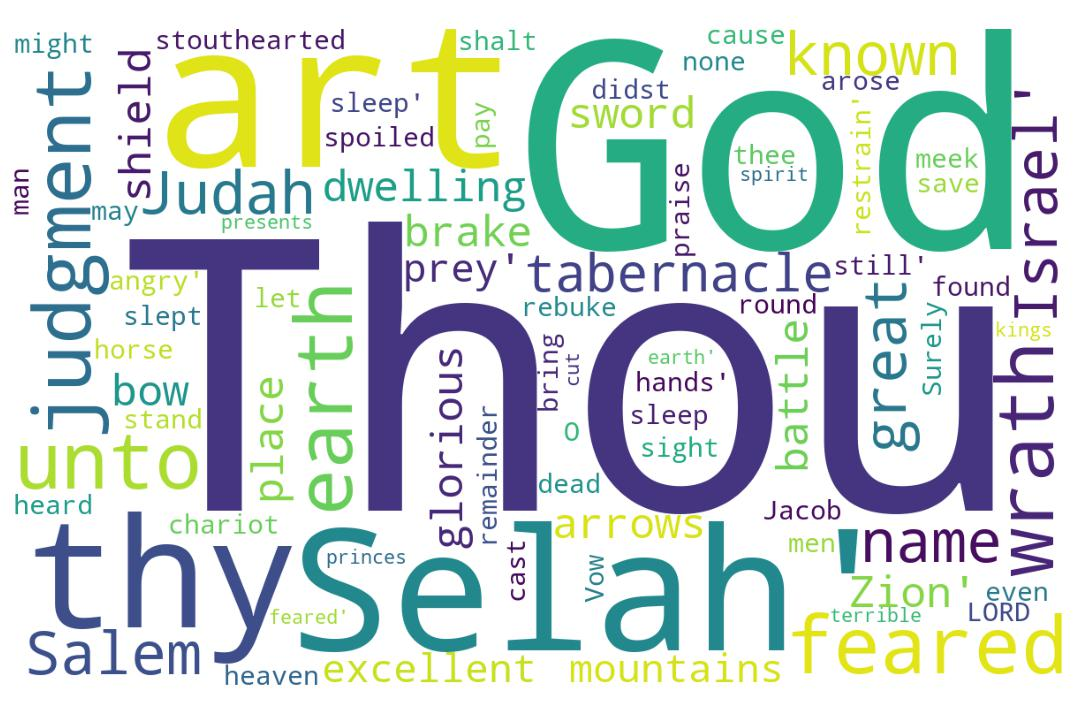
\includegraphics[width=\linewidth]{19OT-Psalms/Psalm76-WordCloud.jpg}
  \caption{Psalm 76 Word Cloud}
  \label{fig:Psalm 76 word Cloud}
\end{figure}

\marginpar{\scriptsize \centering \fcolorbox{bone}{lime}{\textbf{TWO KINDS OF PEOPLE}}\\ (Psalm 76:1-12) \begin{compactenum}[I.][8]
     \item Those \textbf{Shielded} \index[scripture]{Psalms!Psa 076:03}(Psa 76:3)
    \item Those \textbf{Spoiled} \index[scripture]{Psalms!Psa 076:05}(Psa 76:5)
    \item Those \textbf{Put to Sleep} \index[scripture]{Psalms!Psa 076:06}(Psa 76:6)
    \item Those \textbf{Seen} \index[scripture]{Psalms!Psa 076:07}(Psa 76:7)
    \item Those \textbf{Stilled} \index[scripture]{Psalms!Psa 076:08}(Psa 76:8)
    \item Those \textbf{Subdued} \index[scripture]{Psalms!Psa 076:08}(Psa 76:8)
    \item Those \textbf{Saved} \index[scripture]{Psalms!Psa 076:09}(Psa 76:9)
\end{compactenum}}
    




% \textcolor[cmyk]{0.99998,1,0,0}{
\footnote{\textcolor[rgb]{0.00,0.25,0.00}{\hyperlink{TOC}{Return to end of Table of Contents.}}}\footnote{\href{https://audiobible.com/bible/psalms_76.html}{\textcolor[cmyk]{0.99998,1,0,0}{Psalm 76 Audio}}}\textcolor[cmyk]{0.99998,1,0,0}{To the chief Musician on Neginoth, A Psalm \emph{or} Song of Asaph.}\\
\\
\textcolor[cmyk]{0.99998,1,0,0}{In Judah \emph{is} God known: his name \emph{is} great in Israel.} %\footnote{[RUCKMAN] The Psalm is on the Second Advent. God is not known in Judah now, nor has His ``name'' been ``great in Israel'' for 1,950 years. The name “Jehovah” may be great in Israel now, but if we are to believe Deuteronomy 32:15--22; Mark 7:3--13; and Romans 10:1--3, the name is only lip service. God is NOT known, and will not be “known in Judah and Israel” until Hebrews 8:8--12. In this age, God is known, and His “name is great,” among the Gentiles (Acts 28:28), but only because of the Jew (“Judah”). The term “Jew” was given to Judean Jews in Jerusalem (John 5:16, 18), and inspite of tons of anti-Semitic hogwash about “Khazars,” “Edomite usurpers,” and the “ten lost tribes,” salvation is still of the “Jews,” and I don’t mean “Israel” or “the Israel of God” or the “house of Israel.” I mean “Jews,” as in Judean Jews from Judah (vs. 1).\cite{Ruckman1992Psalms}}
[2] \textcolor[cmyk]{0.99998,1,0,0}{In Salem also is his tabernacle, and his dwelling place in Zion.} %\footnote{[RUCKMAN] ``In Salem.” The word is kin to “Shalom” and “Shiloh,” meaning “peace.” God’s dwelling place in this age is NOT in Zion, and He has no tabernacle there; Asaph is prophesying (see the introductory notes). Those who tried to historicize verse 2, and lay it on David or Solomon, have two problems. In the first place, wars do NOT stop in David’s time, nor do they stop in Solomon’s time. The breaking up of weapons in verse 3 is punctuated by our good, old friend “Selah,” showing anyone but a Bible-correcting Hebrew scholar that we are to look at Haggai 2:9 and Zechariah 14 for the meaning of the verse. The word Jerusalem means “city of peace,” so:\cite{Ruckman1992Psalms}
%\begin{compactenum}
%\item It is captured by the Jews in Judges 1:8, but they have to fight against it again to retake it in 2 Samuel 5:6–10. 
%\item Shishak attacks it in 2 Chronicles 12:9.
%\item Jehoash goes after it in 2 Kings 14:13, Rezin in 2 Kings 16:5, and Sennacherib in Isaiah 36 and 37.
%\end{compactenum} 
%Nebuchadnezzar goes up to it three times; Ptolemy Soter attacks it in 320 B.C., Antiochus defiles it in 203 B.C., Scopus attacks it in 199 B.C., and Antiochus hits it again in 168 B.C., and then again “for good measure” in 162 B.C. “City of Peace.” Fantastic, isn’t it? Imagine the commentators thinking that God stopped all the wars with the destruction of David’s foes or Solomon’s or even Hezekiah’s foes (Sennacherib)! Kroll is as tongue tied when he stares at the passage as a calf looking at a “new gate.” He doesn’t know what on earth to do with it. Hyracannus attacks Jerusalem in 65 B.C. Pompey follows suit in 63 B. C. Herod does a bang up job in 39 B.C., and then Titus finishes it off in A.D. 70. But the best is yet to come. Chosroes the Persian attacks it in A.D. 559 after the Romans did it in A.D. 135. Then Afdal takes it in A.D. 1098, after Omar destroyed it in A.D. 637. Then the Crusaders take it (A.D. 1099) only to lose it to Saladin (A.D. 1187). Never fear. Allenby “liberated” it in A.D. 1917, and then the Arabs took over fighting against it with Lebanese, Egyptians, the PLO, the Pope, and the American news media to help them out.\cite{Ruckman1992Psalms}}
[3] \textcolor[cmyk]{0.99998,1,0,0}{There brake he the arrows of the bow, the \fcolorbox{bone}{lime}{shield}, and the sword, and the battle. Selah.}
[4] \textcolor[cmyk]{0.99998,1,0,0}{Thou \emph{art} more glorious \emph{and} excellent than the mountains of prey.} %\footnote{[RUCKMAN] The “thou” is Mt. Zion (see Ps. 68:15 and comments). Two thoughts are present. Mountains which have wild animals on them who take “prey” (Song of Sol. 4:8), are not to be compared with a mountain like Mt. Zion, which not only had the temple on the place where God ordained sacrifices to be made, but also was the location of the Ark of the Covenant which held the Book (Deut. 31:26). The “oracle” of God (1 Kings 6:5) was located on Mt. Zion. The second thought is that the earthly powers represented by mountains (see Rev. 17, for example, and Jeremiah 51:25) are no equal for the “mountain of the Lord” (see Isa. 2:2). He is “king of the mountain,” and His “mountain” will tower above McKinley, Blanc, Whitney, Ararat, Everest, etc., for its prototype (see Heb. 12:22) is already a good bit higher than the entire Milky Way.\cite{Ruckman1992Psalms}}
[5] \textcolor[cmyk]{0.99998,1,0,0}{The stouthearted are \fcolorbox{bone}{lime}{spoiled}, they have slept their sleep: and none of the men of might have found their hands.} %\footnote{[RUCKMAN] Literally, in the sense of Saul (1 Sam. 26:12), who is a type of the Antichrist; doctrinally, in the sense of being dead (see Isa. 26:14; Dan. 12:2). Several things happen at Armageddon that the prophetic expositors never picked up. One of them is that the Antichrist’s troops will kill each other (Judg. 7:22), their flesh will rot on their faces (Zech. 14:12), and their horses will go blind and rabid in the midst of the attack (Zech. 12:4). These are the UN troops (Rev. 19:19) who hope to overthrow the rider on the “white horse” (Rev. 19:10-–14). Observe the advanced revelation found in the AV text which all of the commentators (naturally) missed. When Kroll sees that the “chariot” goes into a dead sleep, as well as the “horses” he mumbles, “the cavalries of the oppressors were stopped.” (Yeah, sonny, they sure were.) The New Idiotic Version (NIV) can’t handle it, so they say that “they lie still.” The Living Baboon says “fell.” The RSV, NRSV, NNRSV (and NNNRSV) take the word “chariot” clean out of the text so they don’t have to deal with the problem: “Both rider and horse lay stunned.” Typical. Absolutely typical of the brand of scholarship you would get at Bob Jones or Liberty University. \cite{Ruckman1992Psalms}}
[6] \textcolor[cmyk]{0.99998,1,0,0}{At thy rebuke, O God of Jacob, both the chariot and horse are cast into a \fcolorbox{bone}{lime}{dead sleep}.} %\footnote{[RUCKMAN] But after 1910, the “chariot” could go to “sleep.” What auto mechanic doesn’t know that? As a matter of fact, the motor can even “die,” and what driver didn’t know that? If it is “awake” but not moving, it is “idling,” and who didn’t know that but the commentators who couldn’t imagine chariots going to sleep? They went to sleep on the Russian front (1942--1944) because the tank fluids froze, or the rats shortcircuited the controls by chewing through the insulation. In my generation (1921--1949), we called automobiles by a peculiar name; we called them “chariots.” A chariot can “malfunction.”\cite{Ruckman1992Psalms}}
[7] \textcolor[cmyk]{0.99998,1,0,0}{Thou, \emph{even} thou, \emph{art} to be feared: and who may stand \fcolorbox{bone}{lime}{in thy sight} when once thou art angry?}
[8] \textcolor[cmyk]{0.99998,1,0,0}{Thou didst cause judgment to be heard from heaven; the earth feared, and was \fcolorbox{bone}{lime}{still}.}
[9] \textcolor[cmyk]{0.99998,1,0,0}{When God arose to judgment, to \fcolorbox{bone}{lime}{save} all the meek of the earth. \fcolorbox{bone}{red}{\textcolor{white}{Selah}}.} %\footnote{[RUCKMAN] All is clear. God “arises” in verse 9 (see Ps. 3:7, 7:6, and 9:19), and not one time is this a reference to God helping anyone out between 500 B. C. and A.D. 2002. “Selah” comes to our aid again to give us the key for judging the critics of the Book. It is a “handy reference” to use in throwing out 80 percent of the rubbish on the Psalms published by Zondervan, Baker, Eerdmans, and Bob Jones University Press. Verse 11 is the exact match for the comments under Psalm 68:29--32, which see. The “vow” of verse 11 is the exact millennial match to Psalm 65:1 and Psalm 50:14, which see. Verse 12 is Armageddon fulfilled, as in Psalm 2:2, 89:27, and Isaiah 24:21. This is a literal destruction at the Advent. In verse 8, we learn that the earth has more sense than most of its inhabitants. The judgment is “heard from heaven,” literally, in Hebrews 12:25; Haggai 2:6; and Psalm 50:3--5 (which see). All of the commentators miss all the references. (This is just as natural for them as breathing.) Note “the meek” of the Sermon on the Mount (Matt. 5:5), showing up in verse 9. \cite{Ruckman1992Psalms}}
[10] \textcolor[cmyk]{0.99998,1,0,0}{Surely the wrath of man shall praise thee: the remainder of wrath shalt thou restrain.} %\footnote{[RUCKMAN ]The destructive critics of the AV come apart at verse 10, which stands in the AV as clear as crystal. The idea is that man’s hatred against God and God’s people will be turned backwards, so that instead of destroying God’s people or stopping God’s hand, God “banks it off the siderail”—He winds up getting glory from it (see Exod. 14:4; Rom. 11:30–34; and Exod. 9:16, 18:11). “The remainder” is a reference to any wrath that does not produce praise for God or glory to Him. Cases are too numerous to mention, the main ones being men killing each other over religious and political issues to the tune of 80,000,000 casualties since A.D. 70. Individual murders (five a day in Detroit, one a day in Las Vegas, two a day in Miami, and ten a day in Washington, D.C.) do not praise God, but murderers are restrained so that total mayhem and murder don’t break out internationally with five hundred killed daily in Memphis, Atlanta, London, Paris, New York, Rome, Madrid, Tokyo, Bombay, Athens, Oslo, Seattle, and Oklahoma City. What wrath does not praise God is held in check so it doesn’t annihilate mankind altogether. Today the Arabs are restrained by “the restrainer” (2 Thess. 2:6–7); otherwise, they would have pushed Israel off into the Mediterranean more than sixty years ago. Kroll (LU) can’t handle it. His peers (Falwell and company) printed a NKJV that reads “you shall gird yourself.” But having made this change, in line with most “highly qualified, recognized Hebrew scholarship” available--used in the RSV, NRSV, and NIV-- they are powerless to interpret the mess they produced, so they leave it there like a rotten egg and print the AV text in the commentary, and then refuse to comment on it! Liberty University inherited its corruption from Edward Wetenhall, the Lord Bishop of Corke and Rosse (1661), Cornelius Buges (1614), and Maurer. These gentlemen tell us that “the Hebrew says....” (Oh, don’t you know. Don’t you just know “the Hebrew says.” I know what “the Hebrew says.” It says whatever the Cult wants you to think it should say. You don’t fool me, kiddies. I used to bartend and lifeguard for a living. You don’t fool me. I’ve shot craps in the alley, played poker “below decks,” got drunk in the French Quarter, and played “cops and teen agers” at all hours of the night. Don’t kid me. I know what the “Hebrew” better say, even if it doesn’t say it.) “Probably it is meant that God girds himself with the praise to which the last of the enemy even to its last remnant is constrained to minister, both in the case of reprobates and....” Yep; that is exactly what it didn’t say, and that is exactly what it didn’t mean. “This, in the Hebrew, is expressed in one word...which imports the begirding or binding of it on every side, that it shall by no means break out, but shall be kept in, as a dog on a chain....” Oh, I got it! He is “held in restraint”! He is a “restrainer”; a leash. Oh yeah, I got “the Hebrew” now! It didn’t mean “gird” at all. It meant “the remainder of wrath shalt thou restrain.” (That’s what I thought you said.) The Living Bible says the “remainder” is an “ornament,” and the Nitty Ickey Version (NIV) says that some “survivors” of God’s wrath are restrained. In the Asinine Standard Vision (ASV), God girds Himself with wrath that came from men instead of Himself. Ditto the Rotten Stupid Version (RSV). Stupidity is infectious. It is passed reverently from one generation of “godly” men to another, so that “historic positions” can overthrow the truth of God in each generation. \cite{Ruckman1992Psalms} }
[11] \textcolor[cmyk]{0.99998,1,0,0}{Vow, and pay unto the LORD your God: let all that be round about him bring presents unto him that ought to be feared.} %\footnote{[RUCKMAN] The ``earth feared'' because the Lord is the One ``that ought to be feared'' (vs. 11). This is for a number of reasons:\cite{Ruckman1992Psalms}
%\begin{compactenum}
%\item He will break all your weapons of war in pieces no matter how “advanced” they are.
%\item He can cast you into a deep sleep (Acts 12:6; Matt. 25:5) when you need to be awake.
%\item He will cut off world rulers, in terror, even if they are ``kings'' and ``princes.''
%\item He can cast you out of His sight and destroy both body and soul in Hell (Matt. 10:28).
%\end{compactenum}}
[12] \textcolor[cmyk]{0.99998,1,0,0}{He shall cut off the spirit of princes: \emph{he} \emph{is} terrible to the kings of the earth.}
\index[NWIV]{11!Psalms!Psa 76:1}\index[AWIP]{In!Psalms!Psa 76:1}\index[AWIP]{Judah!Psalms!Psa 76:1}\index[AWIP]{\emph{is}!Psalms!Psa 76:1}\index[AWIP]{\emph{is}!Psalms!Psa 76:1 (2)}\index[AWIP]{God!Psalms!Psa 76:1}\index[AWIP]{known!Psalms!Psa 76:1}\index[AWIP]{his!Psalms!Psa 76:1}\index[AWIP]{name!Psalms!Psa 76:1}\index[AWIP]{great!Psalms!Psa 76:1}\index[AWIP]{in!Psalms!Psa 76:1}\index[AWIP]{Israel!Psalms!Psa 76:1}\index[AWIP]{\emph{is}!Psalms!Psa 76:1}\index[AWIP]{\emph{is}!Psalms!Psa 76:1 (2)}

\index[NWIV]{12!Psalms!Psa 76:2}\index[AWIP]{In!Psalms!Psa 76:2}\index[AWIP]{Salem!Psalms!Psa 76:2}\index[AWIP]{also!Psalms!Psa 76:2}\index[AWIP]{is!Psalms!Psa 76:2}\index[AWIP]{his!Psalms!Psa 76:2}\index[AWIP]{his!Psalms!Psa 76:2 (2)}\index[AWIP]{tabernacle!Psalms!Psa 76:2}\index[AWIP]{and!Psalms!Psa 76:2}\index[AWIP]{dwelling!Psalms!Psa 76:2}\index[AWIP]{place!Psalms!Psa 76:2}\index[AWIP]{in!Psalms!Psa 76:2}\index[AWIP]{Zion!Psalms!Psa 76:2}

\index[NWIV]{17!Psalms!Psa 76:3}\index[AWIP]{There!Psalms!Psa 76:3}\index[AWIP]{brake!Psalms!Psa 76:3}\index[AWIP]{he!Psalms!Psa 76:3}\index[AWIP]{the!Psalms!Psa 76:3}\index[AWIP]{the!Psalms!Psa 76:3 (2)}\index[AWIP]{the!Psalms!Psa 76:3 (3)}\index[AWIP]{the!Psalms!Psa 76:3 (4)}\index[AWIP]{the!Psalms!Psa 76:3 (5)}\index[AWIP]{arrows!Psalms!Psa 76:3}\index[AWIP]{of!Psalms!Psa 76:3}\index[AWIP]{bow!Psalms!Psa 76:3}\index[AWIP]{shield!Psalms!Psa 76:3}\index[AWIP]{and!Psalms!Psa 76:3}\index[AWIP]{and!Psalms!Psa 76:3 (2)}\index[AWIP]{sword!Psalms!Psa 76:3}\index[AWIP]{battle!Psalms!Psa 76:3}\index[AWIP]{Selah!Psalms!Psa 76:3}

\index[NWIV]{11!Psalms!Psa 76:4}\index[AWIP]{Thou!Psalms!Psa 76:4}\index[AWIP]{\emph{art}!Psalms!Psa 76:4}\index[AWIP]{more!Psalms!Psa 76:4}\index[AWIP]{glorious!Psalms!Psa 76:4}\index[AWIP]{\emph{and}!Psalms!Psa 76:4}\index[AWIP]{excellent!Psalms!Psa 76:4}\index[AWIP]{than!Psalms!Psa 76:4}\index[AWIP]{the!Psalms!Psa 76:4}\index[AWIP]{mountains!Psalms!Psa 76:4}\index[AWIP]{of!Psalms!Psa 76:4}\index[AWIP]{prey!Psalms!Psa 76:4}\index[AWIP]{\emph{art}!Psalms!Psa 76:4}\index[AWIP]{\emph{and}!Psalms!Psa 76:4}

\index[NWIV]{20!Psalms!Psa 76:5}\index[AWIP]{The!Psalms!Psa 76:5}\index[AWIP]{stouthearted!Psalms!Psa 76:5}\index[AWIP]{are!Psalms!Psa 76:5}\index[AWIP]{spoiled!Psalms!Psa 76:5}\index[AWIP]{they!Psalms!Psa 76:5}\index[AWIP]{have!Psalms!Psa 76:5}\index[AWIP]{have!Psalms!Psa 76:5 (2)}\index[AWIP]{slept!Psalms!Psa 76:5}\index[AWIP]{their!Psalms!Psa 76:5}\index[AWIP]{their!Psalms!Psa 76:5 (2)}\index[AWIP]{sleep!Psalms!Psa 76:5}\index[AWIP]{and!Psalms!Psa 76:5}\index[AWIP]{none!Psalms!Psa 76:5}\index[AWIP]{of!Psalms!Psa 76:5}\index[AWIP]{of!Psalms!Psa 76:5 (2)}\index[AWIP]{the!Psalms!Psa 76:5}\index[AWIP]{men!Psalms!Psa 76:5}\index[AWIP]{might!Psalms!Psa 76:5}\index[AWIP]{found!Psalms!Psa 76:5}\index[AWIP]{hands!Psalms!Psa 76:5}

\index[NWIV]{18!Psalms!Psa 76:6}\index[AWIP]{At!Psalms!Psa 76:6}\index[AWIP]{thy!Psalms!Psa 76:6}\index[AWIP]{rebuke!Psalms!Psa 76:6}\index[AWIP]{O!Psalms!Psa 76:6}\index[AWIP]{God!Psalms!Psa 76:6}\index[AWIP]{of!Psalms!Psa 76:6}\index[AWIP]{Jacob!Psalms!Psa 76:6}\index[AWIP]{both!Psalms!Psa 76:6}\index[AWIP]{the!Psalms!Psa 76:6}\index[AWIP]{chariot!Psalms!Psa 76:6}\index[AWIP]{and!Psalms!Psa 76:6}\index[AWIP]{horse!Psalms!Psa 76:6}\index[AWIP]{are!Psalms!Psa 76:6}\index[AWIP]{cast!Psalms!Psa 76:6}\index[AWIP]{into!Psalms!Psa 76:6}\index[AWIP]{a!Psalms!Psa 76:6}\index[AWIP]{dead!Psalms!Psa 76:6}\index[AWIP]{sleep!Psalms!Psa 76:6}

\index[NWIV]{19!Psalms!Psa 76:7}\index[AWIP]{Thou!Psalms!Psa 76:7}\index[AWIP]{\emph{even}!Psalms!Psa 76:7}\index[AWIP]{thou!Psalms!Psa 76:7}\index[AWIP]{thou!Psalms!Psa 76:7 (2)}\index[AWIP]{\emph{art}!Psalms!Psa 76:7}\index[AWIP]{to!Psalms!Psa 76:7}\index[AWIP]{be!Psalms!Psa 76:7}\index[AWIP]{feared!Psalms!Psa 76:7}\index[AWIP]{and!Psalms!Psa 76:7}\index[AWIP]{who!Psalms!Psa 76:7}\index[AWIP]{may!Psalms!Psa 76:7}\index[AWIP]{stand!Psalms!Psa 76:7}\index[AWIP]{in!Psalms!Psa 76:7}\index[AWIP]{thy!Psalms!Psa 76:7}\index[AWIP]{sight!Psalms!Psa 76:7}\index[AWIP]{when!Psalms!Psa 76:7}\index[AWIP]{once!Psalms!Psa 76:7}\index[AWIP]{art!Psalms!Psa 76:7}\index[AWIP]{angry?!Psalms!Psa 76:7}\index[AWIP]{\emph{even}!Psalms!Psa 76:7}\index[AWIP]{\emph{art}!Psalms!Psa 76:7}

\index[NWIV]{15!Psalms!Psa 76:8}\index[AWIP]{Thou!Psalms!Psa 76:8}\index[AWIP]{didst!Psalms!Psa 76:8}\index[AWIP]{cause!Psalms!Psa 76:8}\index[AWIP]{judgment!Psalms!Psa 76:8}\index[AWIP]{to!Psalms!Psa 76:8}\index[AWIP]{be!Psalms!Psa 76:8}\index[AWIP]{heard!Psalms!Psa 76:8}\index[AWIP]{from!Psalms!Psa 76:8}\index[AWIP]{heaven!Psalms!Psa 76:8}\index[AWIP]{the!Psalms!Psa 76:8}\index[AWIP]{earth!Psalms!Psa 76:8}\index[AWIP]{feared!Psalms!Psa 76:8}\index[AWIP]{and!Psalms!Psa 76:8}\index[AWIP]{was!Psalms!Psa 76:8}\index[AWIP]{still!Psalms!Psa 76:8}

\index[NWIV]{14!Psalms!Psa 76:9}\index[AWIP]{When!Psalms!Psa 76:9}\index[AWIP]{God!Psalms!Psa 76:9}\index[AWIP]{arose!Psalms!Psa 76:9}\index[AWIP]{to!Psalms!Psa 76:9}\index[AWIP]{to!Psalms!Psa 76:9 (2)}\index[AWIP]{judgment!Psalms!Psa 76:9}\index[AWIP]{save!Psalms!Psa 76:9}\index[AWIP]{all!Psalms!Psa 76:9}\index[AWIP]{the!Psalms!Psa 76:9}\index[AWIP]{the!Psalms!Psa 76:9 (2)}\index[AWIP]{meek!Psalms!Psa 76:9}\index[AWIP]{of!Psalms!Psa 76:9}\index[AWIP]{earth!Psalms!Psa 76:9}\index[AWIP]{Selah!Psalms!Psa 76:9}

\index[NWIV]{15!Psalms!Psa 76:10}\index[AWIP]{Surely!Psalms!Psa 76:10}\index[AWIP]{the!Psalms!Psa 76:10}\index[AWIP]{the!Psalms!Psa 76:10 (2)}\index[AWIP]{wrath!Psalms!Psa 76:10}\index[AWIP]{wrath!Psalms!Psa 76:10 (2)}\index[AWIP]{of!Psalms!Psa 76:10}\index[AWIP]{of!Psalms!Psa 76:10 (2)}\index[AWIP]{man!Psalms!Psa 76:10}\index[AWIP]{shall!Psalms!Psa 76:10}\index[AWIP]{praise!Psalms!Psa 76:10}\index[AWIP]{thee!Psalms!Psa 76:10}\index[AWIP]{remainder!Psalms!Psa 76:10}\index[AWIP]{shalt!Psalms!Psa 76:10}\index[AWIP]{thou!Psalms!Psa 76:10}\index[AWIP]{restrain!Psalms!Psa 76:10}

\index[NWIV]{24!Psalms!Psa 76:11}\index[AWIP]{Vow!Psalms!Psa 76:11}\index[AWIP]{and!Psalms!Psa 76:11}\index[AWIP]{pay!Psalms!Psa 76:11}\index[AWIP]{unto!Psalms!Psa 76:11}\index[AWIP]{unto!Psalms!Psa 76:11 (2)}\index[AWIP]{the!Psalms!Psa 76:11}\index[AWIP]{LORD!Psalms!Psa 76:11}\index[AWIP]{your!Psalms!Psa 76:11}\index[AWIP]{God!Psalms!Psa 76:11}\index[AWIP]{let!Psalms!Psa 76:11}\index[AWIP]{all!Psalms!Psa 76:11}\index[AWIP]{that!Psalms!Psa 76:11}\index[AWIP]{that!Psalms!Psa 76:11 (2)}\index[AWIP]{be!Psalms!Psa 76:11}\index[AWIP]{be!Psalms!Psa 76:11 (2)}\index[AWIP]{round!Psalms!Psa 76:11}\index[AWIP]{about!Psalms!Psa 76:11}\index[AWIP]{him!Psalms!Psa 76:11}\index[AWIP]{him!Psalms!Psa 76:11 (2)}\index[AWIP]{bring!Psalms!Psa 76:11}\index[AWIP]{presents!Psalms!Psa 76:11}\index[AWIP]{ought!Psalms!Psa 76:11}\index[AWIP]{to!Psalms!Psa 76:11}\index[AWIP]{feared!Psalms!Psa 76:11}

\index[NWIV]{17!Psalms!Psa 76:12}\index[AWIP]{He!Psalms!Psa 76:12}\index[AWIP]{shall!Psalms!Psa 76:12}\index[AWIP]{cut!Psalms!Psa 76:12}\index[AWIP]{off!Psalms!Psa 76:12}\index[AWIP]{the!Psalms!Psa 76:12}\index[AWIP]{the!Psalms!Psa 76:12 (2)}\index[AWIP]{the!Psalms!Psa 76:12 (3)}\index[AWIP]{spirit!Psalms!Psa 76:12}\index[AWIP]{of!Psalms!Psa 76:12}\index[AWIP]{of!Psalms!Psa 76:12 (2)}\index[AWIP]{princes!Psalms!Psa 76:12}\index[AWIP]{\emph{he}!Psalms!Psa 76:12}\index[AWIP]{\emph{is}!Psalms!Psa 76:12}\index[AWIP]{terrible!Psalms!Psa 76:12}\index[AWIP]{to!Psalms!Psa 76:12}\index[AWIP]{kings!Psalms!Psa 76:12}\index[AWIP]{earth!Psalms!Psa 76:12}\index[AWIP]{\emph{he}!Psalms!Psa 76:12}\index[AWIP]{\emph{is}!Psalms!Psa 76:12}


\section{Psalm 76 Outlines}

\subsection{My Outlines}

\subsubsection{Two Kinds of People}

\index[speaker]{Keith Anthony!Psalm 076 (Two Kinds of People)}
\index[series]{Psalms (Keith Anthony)!Psalm 076 (Two Kinds of People)}
\index[date]{2016/08/20!Psalm 076 (Two Kinds of People) (Keith Anthony)}

\begin{compactenum}[I.][7]
    \item Those \textbf{Shielded} \index[scripture]{Psalms!Psa 076:03}(Psa 76:3)
    \item Those \textbf{Spoiled} \index[scripture]{Psalms!Psa 076:05}(Psa 76:5)
    \item Those \textbf{Put to Sleep} \index[scripture]{Psalms!Psa 076:06}(Psa 76:6)
    \item Those \textbf{Seen} \index[scripture]{Psalms!Psa 076:07}(Psa 76:7)
    \item Those \textbf{Stilled} \index[scripture]{Psalms!Psa 076:08}(Psa 76:8)
    \item Those \textbf{Subdued} \index[scripture]{Psalms!Psa 076:08}(Psa 76:8)
    \item Those \textbf{Saved} \index[scripture]{Psalms!Psa 076:09}(Psa 76:9)
\end{compactenum}


\subsection{Outlines from Others}


\section{Psalm 76 Comments}




\subsection{Psalm 75 Repeated Phrases}


%%%%%%%%%%
%%%%%%%%%%
\normalsize
 
\begin{center}
\begin{longtable}{|p{3.0in}|p{0.5in}|}
\caption[Psalm 75 Repeated Phrases]{Psalm 75 Repeated Phrases}\label{table:Repeated Phrases Psalm 75} \\
\hline \multicolumn{1}{|c|}{\textbf{Phrase}} & \multicolumn{1}{c|}{\textbf{Frequency}} \\ \hline 
\endfirsthead
 
\multicolumn{2}{c}
{{\bfseries \tablename\ \thetable{} -- continued from previous page}} \\  
\hline \multicolumn{1}{|c|}{\textbf{Phrase}} & \multicolumn{1}{c|}{\textbf{Frequency}} \\ \hline 
\endhead
 
\hline \multicolumn{2}{c}{{ }} \\ \hline
\endfoot 
of the & 5\\ \hline 
I will & 3\\ \hline 
the wicked & 3\\ \hline 
from the & 3\\ \hline 
\end{longtable}
\end{center}



%%%%%%%%%%
%%%%%%%%%%



\section{Psalm 76 Statistics}

%%%%%%%%%%%%%%%%%%%%%%%%%%%
%%%%% Word Statistics
%%%%%%%%%%%%%%%%%%%%%%%%%%


\normalsize



\subsection{Chapter Word Statistics}


%%%%%%%%%%
%%%%%%%%%%
 
\begin{center}
\begin{longtable}{l|c|c|c|c}
\caption[Stats for Psalm 76]{Stats for Psalm 76} \label{table:Stats for Psalm 76} \\ 
\hline \multicolumn{1}{|c|}{\textbf{Verse(s)}} & \multicolumn{1}{|c|}{\textbf{Count}} & \multicolumn{1}{|c|}{\textbf{Unique}} & \multicolumn{1}{|c|}{\textbf{Italics}} & \multicolumn{1}{|c|}{\textbf{Uniq Italic}}  \\ \hline 
\endfirsthead
 
\multicolumn{5}{c}
{{\bfseries \tablename\ \thetable{} -- continued from previous page}} \\  
\hline \multicolumn{1}{|c|}{\textbf{Verse(s)}} & \multicolumn{1}{|c|}{\textbf{Count}} & \multicolumn{1}{|c|}{\textbf{Unique}} & \multicolumn{1}{|c|}{\textbf{Italics}} & \multicolumn{1}{|c|}{\textbf{Uniq Italic}}  \\ \hline 
\endhead
 
\hline \multicolumn{5}{|r|}{{Continued if needed}} \\ \hline
\endfoot 
1 & 11 & 10 & 2 & 1\\ \hline
2 & 12 & 11 & 0 & 0\\ \hline
3 & 17 & 12 & 0 & 0\\ \hline
4 & 11 & 11 & 2 & 2\\ \hline
5 & 20 & 17 & 0 & 0\\ \hline
6 & 18 & 18 & 0 & 0\\ \hline
7 & 19 & 18 & 2 & 2\\ \hline
8 & 15 & 15 & 0 & 0\\ \hline
9 & 14 & 12 & 0 & 0\\ \hline
10 & 15 & 12 & 0 & 0\\ \hline
11 & 24 & 20 & 0 & 0\\ \hline
12 & 17 & 14 & 2 & 2\\ \hline
\hline \hline
Total & 193 & 121 & 8 & 5



\end{longtable}
\end{center}

%%%%%%%%%%
%%%%%%%%%%
 
\subsection{Words by Frequency}

\begin{center}
\begin{longtable}{l|r}
\caption[Word Frequencies in Psalm 76]{Word Frequencies in Psalm 76} \label{table:WordsIn-Psalm-76} \\ 
\hline \multicolumn{1}{|c|}{\textbf{Word}} & \multicolumn{1}{c|}{\textbf{Frequency}} \\ \hline 
\endfirsthead
 
\multicolumn{2}{c}
{{\bfseries \tablename\ \thetable{} -- continued from previous page}} \\ 
\hline \multicolumn{1}{|c|}{\textbf{Word}} & \multicolumn{1}{c|}{\textbf{Frequency}} \\ \hline 
\endhead
 
\hline \multicolumn{2}{|r|}{{Continued if needed}} \\ \hline
\endfoot
 
\hline \hline
\endlastfoot
the & 17 \\ \hline
of & 10 \\ \hline
and & 8 \\ \hline
to & 6 \\ \hline
God & 4 \\ \hline
be & 4 \\ \hline
\emph{is} & 3 \\ \hline
his & 3 \\ \hline
in & 3 \\ \hline
Thou & 3 \\ \hline
thou & 3 \\ \hline
feared & 3 \\ \hline
earth & 3 \\ \hline
In & 2 \\ \hline
Selah & 2 \\ \hline
\emph{art} & 2 \\ \hline
are & 2 \\ \hline
have & 2 \\ \hline
their & 2 \\ \hline
sleep & 2 \\ \hline
thy & 2 \\ \hline
judgment & 2 \\ \hline
all & 2 \\ \hline
wrath & 2 \\ \hline
shall & 2 \\ \hline
unto & 2 \\ \hline
that & 2 \\ \hline
him & 2 \\ \hline
Judah & 1 \\ \hline
known & 1 \\ \hline
name & 1 \\ \hline
great & 1 \\ \hline
Israel & 1 \\ \hline
Salem & 1 \\ \hline
also & 1 \\ \hline
is & 1 \\ \hline
tabernacle & 1 \\ \hline
dwelling & 1 \\ \hline
place & 1 \\ \hline
Zion & 1 \\ \hline
There & 1 \\ \hline
brake & 1 \\ \hline
he & 1 \\ \hline
arrows & 1 \\ \hline
bow & 1 \\ \hline
shield & 1 \\ \hline
sword & 1 \\ \hline
battle & 1 \\ \hline
more & 1 \\ \hline
glorious & 1 \\ \hline
\emph{and} & 1 \\ \hline
excellent & 1 \\ \hline
than & 1 \\ \hline
mountains & 1 \\ \hline
prey & 1 \\ \hline
The & 1 \\ \hline
stouthearted & 1 \\ \hline
spoiled & 1 \\ \hline
they & 1 \\ \hline
slept & 1 \\ \hline
none & 1 \\ \hline
men & 1 \\ \hline
might & 1 \\ \hline
found & 1 \\ \hline
hands & 1 \\ \hline
At & 1 \\ \hline
rebuke & 1 \\ \hline
O & 1 \\ \hline
Jacob & 1 \\ \hline
both & 1 \\ \hline
chariot & 1 \\ \hline
horse & 1 \\ \hline
cast & 1 \\ \hline
into & 1 \\ \hline
a & 1 \\ \hline
dead & 1 \\ \hline
\emph{even} & 1 \\ \hline
who & 1 \\ \hline
may & 1 \\ \hline
stand & 1 \\ \hline
sight & 1 \\ \hline
when & 1 \\ \hline
once & 1 \\ \hline
art & 1 \\ \hline
angry & 1 \\ \hline
didst & 1 \\ \hline
cause & 1 \\ \hline
heard & 1 \\ \hline
from & 1 \\ \hline
heaven & 1 \\ \hline
was & 1 \\ \hline
still & 1 \\ \hline
When & 1 \\ \hline
arose & 1 \\ \hline
save & 1 \\ \hline
meek & 1 \\ \hline
Surely & 1 \\ \hline
man & 1 \\ \hline
praise & 1 \\ \hline
thee & 1 \\ \hline
remainder & 1 \\ \hline
shalt & 1 \\ \hline
restrain & 1 \\ \hline
Vow & 1 \\ \hline
pay & 1 \\ \hline
LORD & 1 \\ \hline
your & 1 \\ \hline
let & 1 \\ \hline
round & 1 \\ \hline
about & 1 \\ \hline
bring & 1 \\ \hline
presents & 1 \\ \hline
ought & 1 \\ \hline
He & 1 \\ \hline
cut & 1 \\ \hline
off & 1 \\ \hline
spirit & 1 \\ \hline
princes & 1 \\ \hline
\emph{he} & 1 \\ \hline
terrible & 1 \\ \hline
kings & 1 \\ \hline
\end{longtable}
\end{center}



\normalsize



\subsection{Words Alphabetically}

\begin{center}
\begin{longtable}{l|r}
\caption[Word Alphabetically in Psalm 76]{Word Alphabetically in Psalm 76} \label{table:WordsIn-Psalm-76} \\ 
\hline \multicolumn{1}{|c|}{\textbf{Word}} & \multicolumn{1}{c|}{\textbf{Frequency}} \\ \hline 
\endfirsthead
 
\multicolumn{2}{c}
{{\bfseries \tablename\ \thetable{} -- continued from previous page}} \\ 
\hline \multicolumn{1}{|c|}{\textbf{Word}} & \multicolumn{1}{c|}{\textbf{Frequency}} \\ \hline 
\endhead
 
\hline \multicolumn{2}{|r|}{{Continued if needed}} \\ \hline
\endfoot
 
\hline \hline
\endlastfoot
At & 1 \\ \hline
God & 4 \\ \hline
He & 1 \\ \hline
In & 2 \\ \hline
Israel & 1 \\ \hline
Jacob & 1 \\ \hline
Judah & 1 \\ \hline
LORD & 1 \\ \hline
O & 1 \\ \hline
Salem & 1 \\ \hline
Selah & 2 \\ \hline
Surely & 1 \\ \hline
The & 1 \\ \hline
There & 1 \\ \hline
Thou & 3 \\ \hline
Vow & 1 \\ \hline
When & 1 \\ \hline
Zion & 1 \\ \hline
\emph{and} & 1 \\ \hline
\emph{art} & 2 \\ \hline
\emph{even} & 1 \\ \hline
\emph{he} & 1 \\ \hline
\emph{is} & 3 \\ \hline
a & 1 \\ \hline
about & 1 \\ \hline
all & 2 \\ \hline
also & 1 \\ \hline
and & 8 \\ \hline
angry & 1 \\ \hline
are & 2 \\ \hline
arose & 1 \\ \hline
arrows & 1 \\ \hline
art & 1 \\ \hline
battle & 1 \\ \hline
be & 4 \\ \hline
both & 1 \\ \hline
bow & 1 \\ \hline
brake & 1 \\ \hline
bring & 1 \\ \hline
cast & 1 \\ \hline
cause & 1 \\ \hline
chariot & 1 \\ \hline
cut & 1 \\ \hline
dead & 1 \\ \hline
didst & 1 \\ \hline
dwelling & 1 \\ \hline
earth & 3 \\ \hline
excellent & 1 \\ \hline
feared & 3 \\ \hline
found & 1 \\ \hline
from & 1 \\ \hline
glorious & 1 \\ \hline
great & 1 \\ \hline
hands & 1 \\ \hline
have & 2 \\ \hline
he & 1 \\ \hline
heard & 1 \\ \hline
heaven & 1 \\ \hline
him & 2 \\ \hline
his & 3 \\ \hline
horse & 1 \\ \hline
in & 3 \\ \hline
into & 1 \\ \hline
is & 1 \\ \hline
judgment & 2 \\ \hline
kings & 1 \\ \hline
known & 1 \\ \hline
let & 1 \\ \hline
man & 1 \\ \hline
may & 1 \\ \hline
meek & 1 \\ \hline
men & 1 \\ \hline
might & 1 \\ \hline
more & 1 \\ \hline
mountains & 1 \\ \hline
name & 1 \\ \hline
none & 1 \\ \hline
of & 10 \\ \hline
off & 1 \\ \hline
once & 1 \\ \hline
ought & 1 \\ \hline
pay & 1 \\ \hline
place & 1 \\ \hline
praise & 1 \\ \hline
presents & 1 \\ \hline
prey & 1 \\ \hline
princes & 1 \\ \hline
rebuke & 1 \\ \hline
remainder & 1 \\ \hline
restrain & 1 \\ \hline
round & 1 \\ \hline
save & 1 \\ \hline
shall & 2 \\ \hline
shalt & 1 \\ \hline
shield & 1 \\ \hline
sight & 1 \\ \hline
sleep & 2 \\ \hline
slept & 1 \\ \hline
spirit & 1 \\ \hline
spoiled & 1 \\ \hline
stand & 1 \\ \hline
still & 1 \\ \hline
stouthearted & 1 \\ \hline
sword & 1 \\ \hline
tabernacle & 1 \\ \hline
terrible & 1 \\ \hline
than & 1 \\ \hline
that & 2 \\ \hline
the & 17 \\ \hline
thee & 1 \\ \hline
their & 2 \\ \hline
they & 1 \\ \hline
thou & 3 \\ \hline
thy & 2 \\ \hline
to & 6 \\ \hline
unto & 2 \\ \hline
was & 1 \\ \hline
when & 1 \\ \hline
who & 1 \\ \hline
wrath & 2 \\ \hline
your & 1 \\ \hline
\end{longtable}
\end{center}



\normalsize



\subsection{Word Lengths in Chapter}
\normalsize
\begin{longtable}{l|p{3.75in}}
\caption[Words by Length in Psalm 76]{Words by Length in Psalm 76} \label{table:WordsIn-Psalm-76} \\ 
\hline \multicolumn{1}{|c|}{\textbf{Length}} & \multicolumn{1}{c|}{\textbf{Words}} \\ \hline 
\endfirsthead
 
\multicolumn{2}{c}
{{\bfseries \tablename\ \thetable{} -- continued from previous page}} \\ 
\hline \multicolumn{1}{|c|}{\textbf{Length}} & \multicolumn{1}{c|}{\textbf{Words}} \\ \hline 
\endhead
 
\hline \multicolumn{2}{|r|}{{Continued if needed}} \\ \hline
\endfoot
 
\hline \hline
\endlastfoot
1 & O, a \\ \hline
2 & In, \emph{is}, in, is, he, of, At, to, be, He, \emph{he} \\ \hline
3 & God, his, and, the, bow, \emph{art}, \emph{and}, The, are, men, thy, who, may, art, was, all, man, Vow, pay, let, him, cut, off \\ \hline
4 & name, also, Zion, Thou, more, than, prey, they, have, none, both, cast, into, dead, \emph{even}, thou, when, once, from, When, save, meek, thee, unto, LORD, your, that \\ \hline
5 & Judah, known, great, Salem, place, There, brake, sword, Selah, slept, their, sleep, might, found, hands, Jacob, horse, stand, sight, angry, didst, cause, heard, earth, still, arose, wrath, shall, shalt, round, about, bring, ought, kings \\ \hline
6 & Israel, arrows, shield, battle, rebuke, feared, heaven, Surely, praise, spirit \\ \hline
7 & spoiled, chariot, princes \\ \hline
8 & dwelling, glorious, judgment, restrain, presents, terrible \\ \hline
9 & excellent, mountains, remainder \\ \hline
10 & tabernacle \\ \hline
12 & stouthearted \\ \hline
\end{longtable}






%%%%%%%%%%
%%%%%%%%%%
 



%%%%%%%%%%
%%%%%%%%%%
\subsection{Verses with 18 Words in Chapter}
\normalsize
\begin{longtable}{l|p{3.75in}}
\caption[Verses with 18 Words  in Psalm 76]{Verses with 18 Words  in Psalm 76} \label{table:Verses with 18 Words in-Psalm-76} \\ 
\hline \multicolumn{1}{|c|}{\textbf{Reference}} & \multicolumn{1}{c|}{\textbf{Verse}} \\ \hline 
\endfirsthead
 
\multicolumn{2}{c}
{{\bfseries \tablename\ \thetable{} -- continued from previous page}} \\ 
\hline \multicolumn{1}{|c|}{\textbf{Reference}} & \multicolumn{1}{c|}{\textbf{Verse}} \\ \hline 
\endhead
 
\hline \multicolumn{2}{|r|}{{Continued if needed}} \\ \hline
\endfoot
 
\hline \hline
\endlastfoot
Psalms 076:6 & At thy rebuke, O God of Jacob, both the chariot and horse are cast into a dead sleep. \\ \hline
\end{longtable}






%%%%%%%%%%
%%%%%%%%%%

\chapter{Proverb 17}
\begin{figure}
  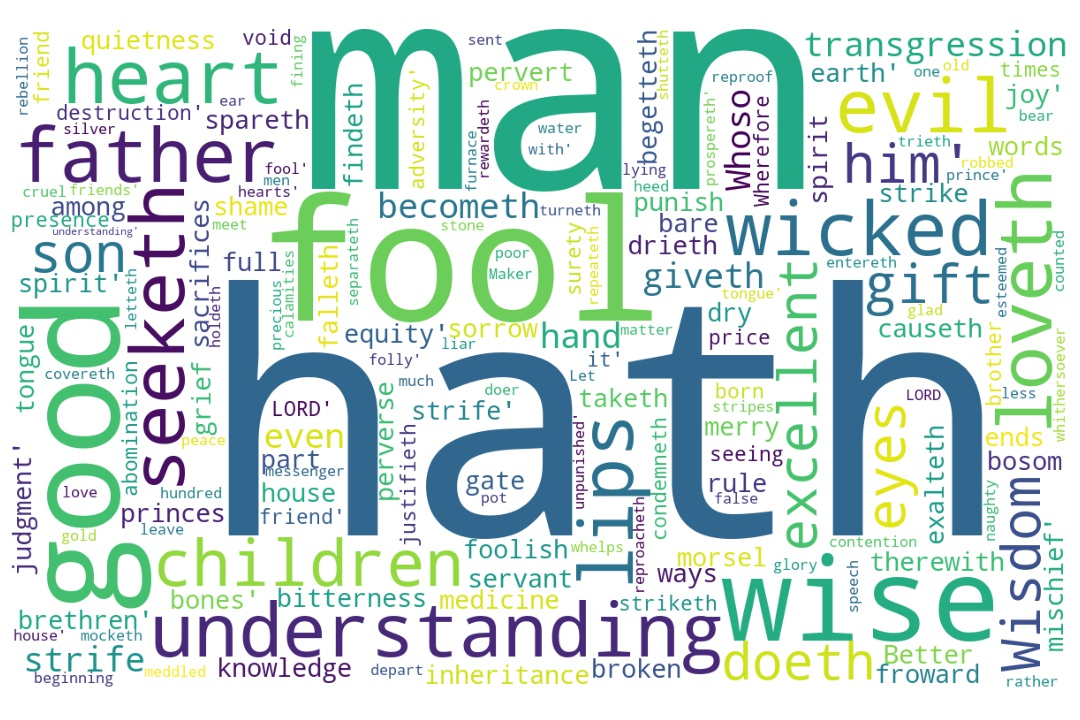
\includegraphics[width=\linewidth]{20OT-Proverbs/Proverb17-WordCloud.jpg}
  \caption{Proverb 17 Word Cloud}
  \label{fig:Proverb 17 word Cloud}
\end{figure}

\marginpar{\scriptsize \centering \fcolorbox{bone}{lime}{\textbf{CONTRASTS}}\\ (Proverbs 17:1-28) \begin{compactenum}[I.][8]
    \item \textbf{A Dry Morsel} \index[scripture]{Proverbs!Pro 17:01}(Pro 17:1) 
    \item \textbf{A Dim-Witted Mocker} \index[scripture]{Proverbs!Pro 17:05}(Pro 17:5) 
    \item \textbf{A Divisive Matter} \index[scripture]{Proverbs!Pro 17:09}(Pro 17:9) 
    \item \textbf{A Disruptive Messenger} \index[scripture]{Proverbs!Pro 17:11}(Pro 17:11) 
    \item \textbf{Destructive Meddling} \index[scripture]{Proverbs!Pro 17:14}(Pro 17:14) 
    \item \textbf{Dangerous Mischief} \index[scripture]{Proverbs!Pro 17:20}(Pro 17:20) 
    \item \textbf{A Discerning Man} \index[scripture]{Proverbs!Pro 17:28} (Pro 17:28) 
\end{compactenum} }

\marginpar{\scriptsize \centering \fcolorbox{bone}{yellow}{\textbf{THE FRUIT OF FOOLS}}\\ (Proverbs 17:1-28) \begin{compactenum}[I.][8]
    \item \textbf{Unwanted Family} \index[scripture]{Proverbs!Pro 17:01}(Pro 17:1) 
    \item \textbf{Unteachable Fool} \index[scripture]{Proverbs!Pro 17:10}(Pro 17:10) 
    \item \textbf{Unstoppable Fool} \index[scripture]{Proverbs!Pro 17:11}(Pro 17:11)  
    \item \textbf{Unrestrained Fanatic} \index[scripture]{Proverbs!Pro 17:11}(Pro 17:11)
    \item \textbf{Uncontrollable Flood} \index[scripture]{Proverbs!Pro 17:14}(Pro 17:14)  
    \item \textbf{Unshakeable Fealty} \index[scripture]{Proverbs!Pro 17:17}(Pro 17:17)  
    \item \textbf{Unfulfilled Father} \index[scripture]{Proverbs!Pro 17:21}(Pro 17:21) 
    \item \textbf{Unobtainable Focus} \index[scripture]{Proverbs!Pro 17:24}(Pro 17:24)  
\end{compactenum} }

\footnote{\textcolor[cmyk]{0.99998,1,0,0}{\hyperlink{TOC}{Return to end of Table of Contents.}}}\footnote{\href{https://audiobible.com/bible/proverbs_17.html}{\textcolor[cmyk]{0.99998,1,0,0}{Proverbs Audio}}}\textcolor[cmyk]{0.99998,1,0,0}{Better \emph{is} a \fcolorbox{bone}{lime}{dry morsel}, and quietness therewith, than an house full of sacrifices \emph{with} strife.}
[2] \textcolor[cmyk]{0.99998,1,0,0}{A wise servant shall have rule over a son that causeth shame, and shall have part of the inheritance among the brethren.}
[3] \textcolor[cmyk]{0.99998,1,0,0}{The fining pot \emph{is} for silver, and the furnace for gold: but the LORD trieth the hearts.}
[4] \textcolor[cmyk]{0.99998,1,0,0}{A wicked doer giveth heed to false lips; \emph{and} a liar giveth ear to a naughty tongue.}
[5] \textcolor[cmyk]{0.99998,1,0,0}{Whoso \fcolorbox{bone}{lime}{mocketh} the poor reproacheth his Maker: \emph{and} he that is glad at calamities shall not be unpunished.}
[6] \textcolor[cmyk]{0.99998,1,0,0}{Children's children \emph{are} the crown of old men; and the glory of children \emph{are} their fathers.}
[7] \textcolor[cmyk]{0.99998,1,0,0}{Excellent speech becometh not a fool: much less do lying lips a prince.}
[8] \textcolor[cmyk]{0.99998,1,0,0}{A gift \emph{is} \emph{as} a precious stone in the eyes of him that hath it: \fcolorbox{bone}{MYGOLD}{whithersoever} it turneth, it prospereth.}
[9] \textcolor[cmyk]{0.99998,1,0,0}{He that covereth a \fcolorbox{bone}{MYGOLD}{transgression} seeketh love; but he that repeateth a matter \fcolorbox{bone}{lime}{separateth} \emph{very} friends.}
[10] \textcolor[cmyk]{0.99998,1,0,0}{A reproof entereth more into a wise man than an hundred stripes into a fool.}
[11] \textcolor[cmyk]{0.99998,1,0,0}{An evil \emph{man} seeketh only rebellion: therefore a \fcolorbox{bone}{lime}{cruel messenger} shall be sent against him.}
[12] \textcolor[cmyk]{0.99998,1,0,0}{Let a bear robbed of her whelps meet a man, rather than a fool in his folly.}
[13] \textcolor[cmyk]{0.99998,1,0,0}{Whoso rewardeth evil for good, evil shall not depart from his house.}
[14] \textcolor[cmyk]{0.99998,1,0,0}{The beginning of strife \emph{is} \emph{as} when one letteth out water: therefore leave off contention, before it be \fcolorbox{bone}{lime}{meddled} with.}
[15] \textcolor[cmyk]{0.99998,1,0,0}{He that justifieth the wicked, and he that condemneth the just, even they both \emph{are} abomination to the LORD.}
[16] \textcolor[cmyk]{0.99998,1,0,0}{Wherefore \emph{is} \emph{there} a price in the hand of a fool to get wisdom, seeing \emph{he} \emph{hath} no heart \emph{to} \emph{it}?}
[17] \textcolor[cmyk]{0.99998,1,0,0}{A friend loveth at all times, and a brother is born for adversity.}
[18] \textcolor[cmyk]{0.99998,1,0,0}{A man void of \fcolorbox{bone}{MYGOLD}{understanding} striketh hands, \emph{and} becometh surety in the presence of his friend.}
[19] \textcolor[cmyk]{0.99998,1,0,0}{He loveth \fcolorbox{bone}{MYGOLD}{transgression} that loveth strife: \emph{and} he that exalteth his gate seeketh destruction.}
[20] \textcolor[cmyk]{0.99998,1,0,0}{He that hath a froward heart findeth no good: and he that hath a perverse tongue falleth into \fcolorbox{bone}{lime}{mischief}.}
[21] \textcolor[cmyk]{0.99998,1,0,0}{He that begetteth a fool \emph{doeth} \emph{it} to his sorrow: and the father of a fool hath no joy.}
[22] \textcolor[cmyk]{0.99998,1,0,0}{A merry heart doeth good \emph{like} a medicine: but a broken spirit drieth the bones.}
[23] \textcolor[cmyk]{0.99998,1,0,0}{A wicked \emph{man} taketh a gift out of the bosom to pervert the ways of judgment.}
[24] \textcolor[cmyk]{0.99998,1,0,0}{Wisdom \emph{is} before him that hath \fcolorbox{bone}{MYGOLD}{understanding}; but the eyes of a fool \emph{are} in the ends of the earth.}
[25] \textcolor[cmyk]{0.99998,1,0,0}{A foolish son \emph{is} a grief to his father, and bitterness to her that bare him.}
[26] \textcolor[cmyk]{0.99998,1,0,0}{Also to punish the just \emph{is} not good, \emph{nor} to strike princes for equity.}
[27] \textcolor[cmyk]{0.99998,1,0,0}{He that hath knowledge spareth his words: \emph{and} a man of \fcolorbox{bone}{MYGOLD}{understanding} is of an excellent spirit.}
[28] \textcolor[cmyk]{0.99998,1,0,0}{Even a fool, when he holdeth his peace, is counted wise: \emph{and} he that shutteth his lips \emph{is} \emph{esteemed} \fcolorbox{bone}{lime}{a man of \fcolorbox{bone}{MYGOLD}{understanding}}.}



\index[NWIV]{16!Proverbs!Pro 17:1}\index[AWIP]{Better!Proverbs!Pro 17:1}\index[AWIP]{\emph{is}!Proverbs!Pro 17:1}\index[AWIP]{a!Proverbs!Pro 17:1}\index[AWIP]{dry!Proverbs!Pro 17:1}\index[AWIP]{morsel!Proverbs!Pro 17:1}\index[AWIP]{and!Proverbs!Pro 17:1}\index[AWIP]{quietness!Proverbs!Pro 17:1}\index[AWIP]{therewith!Proverbs!Pro 17:1}\index[AWIP]{than!Proverbs!Pro 17:1}\index[AWIP]{an!Proverbs!Pro 17:1}\index[AWIP]{house!Proverbs!Pro 17:1}\index[AWIP]{full!Proverbs!Pro 17:1}\index[AWIP]{of!Proverbs!Pro 17:1}\index[AWIP]{sacrifices!Proverbs!Pro 17:1}\index[AWIP]{\emph{with}!Proverbs!Pro 17:1}\index[AWIP]{strife!Proverbs!Pro 17:1}\index[AWIP]{\emph{is}!Proverbs!Pro 17:1}\index[AWIP]{\emph{with}!Proverbs!Pro 17:1}

\index[NWIV]{22!Proverbs!Pro 17:2}\index[AWIP]{A!Proverbs!Pro 17:2}\index[AWIP]{wise!Proverbs!Pro 17:2}\index[AWIP]{servant!Proverbs!Pro 17:2}\index[AWIP]{shall!Proverbs!Pro 17:2}\index[AWIP]{shall!Proverbs!Pro 17:2 (2)}\index[AWIP]{have!Proverbs!Pro 17:2}\index[AWIP]{have!Proverbs!Pro 17:2 (2)}\index[AWIP]{rule!Proverbs!Pro 17:2}\index[AWIP]{over!Proverbs!Pro 17:2}\index[AWIP]{a!Proverbs!Pro 17:2}\index[AWIP]{son!Proverbs!Pro 17:2}\index[AWIP]{that!Proverbs!Pro 17:2}\index[AWIP]{causeth!Proverbs!Pro 17:2}\index[AWIP]{shame!Proverbs!Pro 17:2}\index[AWIP]{and!Proverbs!Pro 17:2}\index[AWIP]{part!Proverbs!Pro 17:2}\index[AWIP]{of!Proverbs!Pro 17:2}\index[AWIP]{the!Proverbs!Pro 17:2}\index[AWIP]{the!Proverbs!Pro 17:2 (2)}\index[AWIP]{inheritance!Proverbs!Pro 17:2}\index[AWIP]{among!Proverbs!Pro 17:2}\index[AWIP]{brethren!Proverbs!Pro 17:2}

\index[NWIV]{17!Proverbs!Pro 17:3}\index[AWIP]{The!Proverbs!Pro 17:3}\index[AWIP]{fining!Proverbs!Pro 17:3}\index[AWIP]{pot!Proverbs!Pro 17:3}\index[AWIP]{\emph{is}!Proverbs!Pro 17:3}\index[AWIP]{for!Proverbs!Pro 17:3}\index[AWIP]{for!Proverbs!Pro 17:3 (2)}\index[AWIP]{silver!Proverbs!Pro 17:3}\index[AWIP]{and!Proverbs!Pro 17:3}\index[AWIP]{the!Proverbs!Pro 17:3}\index[AWIP]{the!Proverbs!Pro 17:3 (2)}\index[AWIP]{the!Proverbs!Pro 17:3 (3)}\index[AWIP]{furnace!Proverbs!Pro 17:3}\index[AWIP]{gold!Proverbs!Pro 17:3}\index[AWIP]{but!Proverbs!Pro 17:3}\index[AWIP]{LORD!Proverbs!Pro 17:3}\index[AWIP]{trieth!Proverbs!Pro 17:3}\index[AWIP]{hearts!Proverbs!Pro 17:3}\index[AWIP]{\emph{is}!Proverbs!Pro 17:3}

\index[NWIV]{17!Proverbs!Pro 17:4}\index[AWIP]{A!Proverbs!Pro 17:4}\index[AWIP]{wicked!Proverbs!Pro 17:4}\index[AWIP]{doer!Proverbs!Pro 17:4}\index[AWIP]{giveth!Proverbs!Pro 17:4}\index[AWIP]{giveth!Proverbs!Pro 17:4 (2)}\index[AWIP]{heed!Proverbs!Pro 17:4}\index[AWIP]{to!Proverbs!Pro 17:4}\index[AWIP]{to!Proverbs!Pro 17:4 (2)}\index[AWIP]{false!Proverbs!Pro 17:4}\index[AWIP]{lips!Proverbs!Pro 17:4}\index[AWIP]{\emph{and}!Proverbs!Pro 17:4}\index[AWIP]{a!Proverbs!Pro 17:4}\index[AWIP]{a!Proverbs!Pro 17:4 (2)}\index[AWIP]{liar!Proverbs!Pro 17:4}\index[AWIP]{ear!Proverbs!Pro 17:4}\index[AWIP]{naughty!Proverbs!Pro 17:4}\index[AWIP]{tongue!Proverbs!Pro 17:4}\index[AWIP]{\emph{and}!Proverbs!Pro 17:4}

\index[NWIV]{18!Proverbs!Pro 17:5}\index[AWIP]{Whoso!Proverbs!Pro 17:5}\index[AWIP]{mocketh!Proverbs!Pro 17:5}\index[AWIP]{the!Proverbs!Pro 17:5}\index[AWIP]{poor!Proverbs!Pro 17:5}\index[AWIP]{reproacheth!Proverbs!Pro 17:5}\index[AWIP]{his!Proverbs!Pro 17:5}\index[AWIP]{Maker!Proverbs!Pro 17:5}\index[AWIP]{\emph{and}!Proverbs!Pro 17:5}\index[AWIP]{he!Proverbs!Pro 17:5}\index[AWIP]{that!Proverbs!Pro 17:5}\index[AWIP]{is!Proverbs!Pro 17:5}\index[AWIP]{glad!Proverbs!Pro 17:5}\index[AWIP]{at!Proverbs!Pro 17:5}\index[AWIP]{calamities!Proverbs!Pro 17:5}\index[AWIP]{shall!Proverbs!Pro 17:5}\index[AWIP]{not!Proverbs!Pro 17:5}\index[AWIP]{be!Proverbs!Pro 17:5}\index[AWIP]{unpunished!Proverbs!Pro 17:5}\index[AWIP]{\emph{and}!Proverbs!Pro 17:5}

\index[NWIV]{16!Proverbs!Pro 17:6}\index[AWIP]{Children's!Proverbs!Pro 17:6}\index[AWIP]{children!Proverbs!Pro 17:6}\index[AWIP]{children!Proverbs!Pro 17:6 (2)}\index[AWIP]{\emph{are}!Proverbs!Pro 17:6}\index[AWIP]{\emph{are}!Proverbs!Pro 17:6 (2)}\index[AWIP]{the!Proverbs!Pro 17:6}\index[AWIP]{the!Proverbs!Pro 17:6 (2)}\index[AWIP]{crown!Proverbs!Pro 17:6}\index[AWIP]{of!Proverbs!Pro 17:6}\index[AWIP]{of!Proverbs!Pro 17:6 (2)}\index[AWIP]{old!Proverbs!Pro 17:6}\index[AWIP]{men!Proverbs!Pro 17:6}\index[AWIP]{and!Proverbs!Pro 17:6}\index[AWIP]{glory!Proverbs!Pro 17:6}\index[AWIP]{their!Proverbs!Pro 17:6}\index[AWIP]{fathers!Proverbs!Pro 17:6}\index[AWIP]{\emph{are}!Proverbs!Pro 17:6}\index[AWIP]{\emph{are}!Proverbs!Pro 17:6 (2)}

\index[NWIV]{13!Proverbs!Pro 17:7}\index[AWIP]{Excellent!Proverbs!Pro 17:7}\index[AWIP]{speech!Proverbs!Pro 17:7}\index[AWIP]{becometh!Proverbs!Pro 17:7}\index[AWIP]{not!Proverbs!Pro 17:7}\index[AWIP]{a!Proverbs!Pro 17:7}\index[AWIP]{a!Proverbs!Pro 17:7 (2)}\index[AWIP]{fool!Proverbs!Pro 17:7}\index[AWIP]{much!Proverbs!Pro 17:7}\index[AWIP]{less!Proverbs!Pro 17:7}\index[AWIP]{do!Proverbs!Pro 17:7}\index[AWIP]{lying!Proverbs!Pro 17:7}\index[AWIP]{lips!Proverbs!Pro 17:7}\index[AWIP]{prince!Proverbs!Pro 17:7}

\index[NWIV]{20!Proverbs!Pro 17:8}\index[AWIP]{A!Proverbs!Pro 17:8}\index[AWIP]{gift!Proverbs!Pro 17:8}\index[AWIP]{\emph{is}!Proverbs!Pro 17:8}\index[AWIP]{\emph{as}!Proverbs!Pro 17:8}\index[AWIP]{a!Proverbs!Pro 17:8}\index[AWIP]{precious!Proverbs!Pro 17:8}\index[AWIP]{stone!Proverbs!Pro 17:8}\index[AWIP]{in!Proverbs!Pro 17:8}\index[AWIP]{the!Proverbs!Pro 17:8}\index[AWIP]{eyes!Proverbs!Pro 17:8}\index[AWIP]{of!Proverbs!Pro 17:8}\index[AWIP]{him!Proverbs!Pro 17:8}\index[AWIP]{that!Proverbs!Pro 17:8}\index[AWIP]{hath!Proverbs!Pro 17:8}\index[AWIP]{it!Proverbs!Pro 17:8}\index[AWIP]{it!Proverbs!Pro 17:8 (2)}\index[AWIP]{it!Proverbs!Pro 17:8 (3)}\index[AWIP]{whithersoever!Proverbs!Pro 17:8}\index[AWIP]{turneth!Proverbs!Pro 17:8}\index[AWIP]{prospereth!Proverbs!Pro 17:8}\index[AWIP]{\emph{is}!Proverbs!Pro 17:8}\index[AWIP]{\emph{as}!Proverbs!Pro 17:8}

\index[NWIV]{16!Proverbs!Pro 17:9}\index[AWIP]{He!Proverbs!Pro 17:9}\index[AWIP]{that!Proverbs!Pro 17:9}\index[AWIP]{that!Proverbs!Pro 17:9 (2)}\index[AWIP]{covereth!Proverbs!Pro 17:9}\index[AWIP]{a!Proverbs!Pro 17:9}\index[AWIP]{a!Proverbs!Pro 17:9 (2)}\index[AWIP]{transgression!Proverbs!Pro 17:9}\index[AWIP]{seeketh!Proverbs!Pro 17:9}\index[AWIP]{love!Proverbs!Pro 17:9}\index[AWIP]{but!Proverbs!Pro 17:9}\index[AWIP]{he!Proverbs!Pro 17:9}\index[AWIP]{repeateth!Proverbs!Pro 17:9}\index[AWIP]{matter!Proverbs!Pro 17:9}\index[AWIP]{separateth!Proverbs!Pro 17:9}\index[AWIP]{\emph{very}!Proverbs!Pro 17:9}\index[AWIP]{friends!Proverbs!Pro 17:9}\index[AWIP]{\emph{very}!Proverbs!Pro 17:9}

\index[NWIV]{15!Proverbs!Pro 17:10}\index[AWIP]{A!Proverbs!Pro 17:10}\index[AWIP]{reproof!Proverbs!Pro 17:10}\index[AWIP]{entereth!Proverbs!Pro 17:10}\index[AWIP]{more!Proverbs!Pro 17:10}\index[AWIP]{into!Proverbs!Pro 17:10}\index[AWIP]{into!Proverbs!Pro 17:10 (2)}\index[AWIP]{a!Proverbs!Pro 17:10}\index[AWIP]{a!Proverbs!Pro 17:10 (2)}\index[AWIP]{wise!Proverbs!Pro 17:10}\index[AWIP]{man!Proverbs!Pro 17:10}\index[AWIP]{than!Proverbs!Pro 17:10}\index[AWIP]{an!Proverbs!Pro 17:10}\index[AWIP]{hundred!Proverbs!Pro 17:10}\index[AWIP]{stripes!Proverbs!Pro 17:10}\index[AWIP]{fool!Proverbs!Pro 17:10}

\index[NWIV]{15!Proverbs!Pro 17:11}\index[AWIP]{An!Proverbs!Pro 17:11}\index[AWIP]{evil!Proverbs!Pro 17:11}\index[AWIP]{\emph{man}!Proverbs!Pro 17:11}\index[AWIP]{seeketh!Proverbs!Pro 17:11}\index[AWIP]{only!Proverbs!Pro 17:11}\index[AWIP]{rebellion!Proverbs!Pro 17:11}\index[AWIP]{therefore!Proverbs!Pro 17:11}\index[AWIP]{a!Proverbs!Pro 17:11}\index[AWIP]{cruel!Proverbs!Pro 17:11}\index[AWIP]{messenger!Proverbs!Pro 17:11}\index[AWIP]{shall!Proverbs!Pro 17:11}\index[AWIP]{be!Proverbs!Pro 17:11}\index[AWIP]{sent!Proverbs!Pro 17:11}\index[AWIP]{against!Proverbs!Pro 17:11}\index[AWIP]{him!Proverbs!Pro 17:11}\index[AWIP]{\emph{man}!Proverbs!Pro 17:11}

\index[NWIV]{17!Proverbs!Pro 17:12}\index[AWIP]{Let!Proverbs!Pro 17:12}\index[AWIP]{a!Proverbs!Pro 17:12}\index[AWIP]{a!Proverbs!Pro 17:12 (2)}\index[AWIP]{a!Proverbs!Pro 17:12 (3)}\index[AWIP]{bear!Proverbs!Pro 17:12}\index[AWIP]{robbed!Proverbs!Pro 17:12}\index[AWIP]{of!Proverbs!Pro 17:12}\index[AWIP]{her!Proverbs!Pro 17:12}\index[AWIP]{whelps!Proverbs!Pro 17:12}\index[AWIP]{meet!Proverbs!Pro 17:12}\index[AWIP]{man!Proverbs!Pro 17:12}\index[AWIP]{rather!Proverbs!Pro 17:12}\index[AWIP]{than!Proverbs!Pro 17:12}\index[AWIP]{fool!Proverbs!Pro 17:12}\index[AWIP]{in!Proverbs!Pro 17:12}\index[AWIP]{his!Proverbs!Pro 17:12}\index[AWIP]{folly!Proverbs!Pro 17:12}

\index[NWIV]{12!Proverbs!Pro 17:13}\index[AWIP]{Whoso!Proverbs!Pro 17:13}\index[AWIP]{rewardeth!Proverbs!Pro 17:13}\index[AWIP]{evil!Proverbs!Pro 17:13}\index[AWIP]{evil!Proverbs!Pro 17:13 (2)}\index[AWIP]{for!Proverbs!Pro 17:13}\index[AWIP]{good!Proverbs!Pro 17:13}\index[AWIP]{shall!Proverbs!Pro 17:13}\index[AWIP]{not!Proverbs!Pro 17:13}\index[AWIP]{depart!Proverbs!Pro 17:13}\index[AWIP]{from!Proverbs!Pro 17:13}\index[AWIP]{his!Proverbs!Pro 17:13}\index[AWIP]{house!Proverbs!Pro 17:13}

\index[NWIV]{20!Proverbs!Pro 17:14}\index[AWIP]{The!Proverbs!Pro 17:14}\index[AWIP]{beginning!Proverbs!Pro 17:14}\index[AWIP]{of!Proverbs!Pro 17:14}\index[AWIP]{strife!Proverbs!Pro 17:14}\index[AWIP]{\emph{is}!Proverbs!Pro 17:14}\index[AWIP]{\emph{as}!Proverbs!Pro 17:14}\index[AWIP]{when!Proverbs!Pro 17:14}\index[AWIP]{one!Proverbs!Pro 17:14}\index[AWIP]{letteth!Proverbs!Pro 17:14}\index[AWIP]{out!Proverbs!Pro 17:14}\index[AWIP]{water!Proverbs!Pro 17:14}\index[AWIP]{therefore!Proverbs!Pro 17:14}\index[AWIP]{leave!Proverbs!Pro 17:14}\index[AWIP]{off!Proverbs!Pro 17:14}\index[AWIP]{contention!Proverbs!Pro 17:14}\index[AWIP]{before!Proverbs!Pro 17:14}\index[AWIP]{it!Proverbs!Pro 17:14}\index[AWIP]{be!Proverbs!Pro 17:14}\index[AWIP]{meddled!Proverbs!Pro 17:14}\index[AWIP]{with!Proverbs!Pro 17:14}\index[AWIP]{\emph{is}!Proverbs!Pro 17:14}\index[AWIP]{\emph{as}!Proverbs!Pro 17:14}

\index[NWIV]{19!Proverbs!Pro 17:15}\index[AWIP]{He!Proverbs!Pro 17:15}\index[AWIP]{that!Proverbs!Pro 17:15}\index[AWIP]{that!Proverbs!Pro 17:15 (2)}\index[AWIP]{justifieth!Proverbs!Pro 17:15}\index[AWIP]{the!Proverbs!Pro 17:15}\index[AWIP]{the!Proverbs!Pro 17:15 (2)}\index[AWIP]{the!Proverbs!Pro 17:15 (3)}\index[AWIP]{wicked!Proverbs!Pro 17:15}\index[AWIP]{and!Proverbs!Pro 17:15}\index[AWIP]{he!Proverbs!Pro 17:15}\index[AWIP]{condemneth!Proverbs!Pro 17:15}\index[AWIP]{just!Proverbs!Pro 17:15}\index[AWIP]{even!Proverbs!Pro 17:15}\index[AWIP]{they!Proverbs!Pro 17:15}\index[AWIP]{both!Proverbs!Pro 17:15}\index[AWIP]{\emph{are}!Proverbs!Pro 17:15}\index[AWIP]{abomination!Proverbs!Pro 17:15}\index[AWIP]{to!Proverbs!Pro 17:15}\index[AWIP]{LORD!Proverbs!Pro 17:15}\index[AWIP]{\emph{are}!Proverbs!Pro 17:15}

\index[NWIV]{21!Proverbs!Pro 17:16}\index[AWIP]{Wherefore!Proverbs!Pro 17:16}\index[AWIP]{\emph{is}!Proverbs!Pro 17:16}\index[AWIP]{\emph{there}!Proverbs!Pro 17:16}\index[AWIP]{a!Proverbs!Pro 17:16}\index[AWIP]{a!Proverbs!Pro 17:16 (2)}\index[AWIP]{price!Proverbs!Pro 17:16}\index[AWIP]{in!Proverbs!Pro 17:16}\index[AWIP]{the!Proverbs!Pro 17:16}\index[AWIP]{hand!Proverbs!Pro 17:16}\index[AWIP]{of!Proverbs!Pro 17:16}\index[AWIP]{fool!Proverbs!Pro 17:16}\index[AWIP]{to!Proverbs!Pro 17:16}\index[AWIP]{get!Proverbs!Pro 17:16}\index[AWIP]{wisdom!Proverbs!Pro 17:16}\index[AWIP]{seeing!Proverbs!Pro 17:16}\index[AWIP]{\emph{he}!Proverbs!Pro 17:16}\index[AWIP]{\emph{hath}!Proverbs!Pro 17:16}\index[AWIP]{no!Proverbs!Pro 17:16}\index[AWIP]{heart!Proverbs!Pro 17:16}\index[AWIP]{\emph{to}!Proverbs!Pro 17:16}\index[AWIP]{\emph{it}?!Proverbs!Pro 17:16}\index[AWIP]{\emph{is}!Proverbs!Pro 17:16}\index[AWIP]{\emph{there}!Proverbs!Pro 17:16}\index[AWIP]{\emph{he}!Proverbs!Pro 17:16}\index[AWIP]{\emph{hath}!Proverbs!Pro 17:16}\index[AWIP]{\emph{to}!Proverbs!Pro 17:16}\index[AWIP]{\emph{it}?!Proverbs!Pro 17:16}

\index[NWIV]{13!Proverbs!Pro 17:17}\index[AWIP]{A!Proverbs!Pro 17:17}\index[AWIP]{friend!Proverbs!Pro 17:17}\index[AWIP]{loveth!Proverbs!Pro 17:17}\index[AWIP]{at!Proverbs!Pro 17:17}\index[AWIP]{all!Proverbs!Pro 17:17}\index[AWIP]{times!Proverbs!Pro 17:17}\index[AWIP]{and!Proverbs!Pro 17:17}\index[AWIP]{a!Proverbs!Pro 17:17}\index[AWIP]{brother!Proverbs!Pro 17:17}\index[AWIP]{is!Proverbs!Pro 17:17}\index[AWIP]{born!Proverbs!Pro 17:17}\index[AWIP]{for!Proverbs!Pro 17:17}\index[AWIP]{adversity!Proverbs!Pro 17:17}

\index[NWIV]{16!Proverbs!Pro 17:18}\index[AWIP]{A!Proverbs!Pro 17:18}\index[AWIP]{man!Proverbs!Pro 17:18}\index[AWIP]{void!Proverbs!Pro 17:18}\index[AWIP]{of!Proverbs!Pro 17:18}\index[AWIP]{of!Proverbs!Pro 17:18 (2)}\index[AWIP]{understanding!Proverbs!Pro 17:18}\index[AWIP]{striketh!Proverbs!Pro 17:18}\index[AWIP]{hands!Proverbs!Pro 17:18}\index[AWIP]{\emph{and}!Proverbs!Pro 17:18}\index[AWIP]{becometh!Proverbs!Pro 17:18}\index[AWIP]{surety!Proverbs!Pro 17:18}\index[AWIP]{in!Proverbs!Pro 17:18}\index[AWIP]{the!Proverbs!Pro 17:18}\index[AWIP]{presence!Proverbs!Pro 17:18}\index[AWIP]{his!Proverbs!Pro 17:18}\index[AWIP]{friend!Proverbs!Pro 17:18}\index[AWIP]{\emph{and}!Proverbs!Pro 17:18}

\index[NWIV]{14!Proverbs!Pro 17:19}\index[AWIP]{He!Proverbs!Pro 17:19}\index[AWIP]{loveth!Proverbs!Pro 17:19}\index[AWIP]{loveth!Proverbs!Pro 17:19 (2)}\index[AWIP]{transgression!Proverbs!Pro 17:19}\index[AWIP]{that!Proverbs!Pro 17:19}\index[AWIP]{that!Proverbs!Pro 17:19 (2)}\index[AWIP]{strife!Proverbs!Pro 17:19}\index[AWIP]{\emph{and}!Proverbs!Pro 17:19}\index[AWIP]{he!Proverbs!Pro 17:19}\index[AWIP]{exalteth!Proverbs!Pro 17:19}\index[AWIP]{his!Proverbs!Pro 17:19}\index[AWIP]{gate!Proverbs!Pro 17:19}\index[AWIP]{seeketh!Proverbs!Pro 17:19}\index[AWIP]{destruction!Proverbs!Pro 17:19}\index[AWIP]{\emph{and}!Proverbs!Pro 17:19}

\index[NWIV]{19!Proverbs!Pro 17:20}\index[AWIP]{He!Proverbs!Pro 17:20}\index[AWIP]{that!Proverbs!Pro 17:20}\index[AWIP]{that!Proverbs!Pro 17:20 (2)}\index[AWIP]{hath!Proverbs!Pro 17:20}\index[AWIP]{hath!Proverbs!Pro 17:20 (2)}\index[AWIP]{a!Proverbs!Pro 17:20}\index[AWIP]{a!Proverbs!Pro 17:20 (2)}\index[AWIP]{froward!Proverbs!Pro 17:20}\index[AWIP]{heart!Proverbs!Pro 17:20}\index[AWIP]{findeth!Proverbs!Pro 17:20}\index[AWIP]{no!Proverbs!Pro 17:20}\index[AWIP]{good!Proverbs!Pro 17:20}\index[AWIP]{and!Proverbs!Pro 17:20}\index[AWIP]{he!Proverbs!Pro 17:20}\index[AWIP]{perverse!Proverbs!Pro 17:20}\index[AWIP]{tongue!Proverbs!Pro 17:20}\index[AWIP]{falleth!Proverbs!Pro 17:20}\index[AWIP]{into!Proverbs!Pro 17:20}\index[AWIP]{mischief!Proverbs!Pro 17:20}

\index[NWIV]{19!Proverbs!Pro 17:21}\index[AWIP]{He!Proverbs!Pro 17:21}\index[AWIP]{that!Proverbs!Pro 17:21}\index[AWIP]{begetteth!Proverbs!Pro 17:21}\index[AWIP]{a!Proverbs!Pro 17:21}\index[AWIP]{a!Proverbs!Pro 17:21 (2)}\index[AWIP]{fool!Proverbs!Pro 17:21}\index[AWIP]{fool!Proverbs!Pro 17:21 (2)}\index[AWIP]{\emph{doeth}!Proverbs!Pro 17:21}\index[AWIP]{\emph{it}!Proverbs!Pro 17:21}\index[AWIP]{to!Proverbs!Pro 17:21}\index[AWIP]{his!Proverbs!Pro 17:21}\index[AWIP]{sorrow!Proverbs!Pro 17:21}\index[AWIP]{and!Proverbs!Pro 17:21}\index[AWIP]{the!Proverbs!Pro 17:21}\index[AWIP]{father!Proverbs!Pro 17:21}\index[AWIP]{of!Proverbs!Pro 17:21}\index[AWIP]{hath!Proverbs!Pro 17:21}\index[AWIP]{no!Proverbs!Pro 17:21}\index[AWIP]{joy!Proverbs!Pro 17:21}\index[AWIP]{\emph{doeth}!Proverbs!Pro 17:21}\index[AWIP]{\emph{it}!Proverbs!Pro 17:21}

\index[NWIV]{15!Proverbs!Pro 17:22}\index[AWIP]{A!Proverbs!Pro 17:22}\index[AWIP]{merry!Proverbs!Pro 17:22}\index[AWIP]{heart!Proverbs!Pro 17:22}\index[AWIP]{doeth!Proverbs!Pro 17:22}\index[AWIP]{good!Proverbs!Pro 17:22}\index[AWIP]{\emph{like}!Proverbs!Pro 17:22}\index[AWIP]{a!Proverbs!Pro 17:22}\index[AWIP]{a!Proverbs!Pro 17:22 (2)}\index[AWIP]{medicine!Proverbs!Pro 17:22}\index[AWIP]{but!Proverbs!Pro 17:22}\index[AWIP]{broken!Proverbs!Pro 17:22}\index[AWIP]{spirit!Proverbs!Pro 17:22}\index[AWIP]{drieth!Proverbs!Pro 17:22}\index[AWIP]{the!Proverbs!Pro 17:22}\index[AWIP]{bones!Proverbs!Pro 17:22}\index[AWIP]{\emph{like}!Proverbs!Pro 17:22}

\index[NWIV]{16!Proverbs!Pro 17:23}\index[AWIP]{A!Proverbs!Pro 17:23}\index[AWIP]{wicked!Proverbs!Pro 17:23}\index[AWIP]{\emph{man}!Proverbs!Pro 17:23}\index[AWIP]{taketh!Proverbs!Pro 17:23}\index[AWIP]{a!Proverbs!Pro 17:23}\index[AWIP]{gift!Proverbs!Pro 17:23}\index[AWIP]{out!Proverbs!Pro 17:23}\index[AWIP]{of!Proverbs!Pro 17:23}\index[AWIP]{of!Proverbs!Pro 17:23 (2)}\index[AWIP]{the!Proverbs!Pro 17:23}\index[AWIP]{the!Proverbs!Pro 17:23 (2)}\index[AWIP]{bosom!Proverbs!Pro 17:23}\index[AWIP]{to!Proverbs!Pro 17:23}\index[AWIP]{pervert!Proverbs!Pro 17:23}\index[AWIP]{ways!Proverbs!Pro 17:23}\index[AWIP]{judgment!Proverbs!Pro 17:23}\index[AWIP]{\emph{man}!Proverbs!Pro 17:23}

\index[NWIV]{20!Proverbs!Pro 17:24}\index[AWIP]{Wisdom!Proverbs!Pro 17:24}\index[AWIP]{\emph{is}!Proverbs!Pro 17:24}\index[AWIP]{before!Proverbs!Pro 17:24}\index[AWIP]{him!Proverbs!Pro 17:24}\index[AWIP]{that!Proverbs!Pro 17:24}\index[AWIP]{hath!Proverbs!Pro 17:24}\index[AWIP]{understanding!Proverbs!Pro 17:24}\index[AWIP]{but!Proverbs!Pro 17:24}\index[AWIP]{the!Proverbs!Pro 17:24}\index[AWIP]{the!Proverbs!Pro 17:24 (2)}\index[AWIP]{the!Proverbs!Pro 17:24 (3)}\index[AWIP]{eyes!Proverbs!Pro 17:24}\index[AWIP]{of!Proverbs!Pro 17:24}\index[AWIP]{of!Proverbs!Pro 17:24 (2)}\index[AWIP]{a!Proverbs!Pro 17:24}\index[AWIP]{fool!Proverbs!Pro 17:24}\index[AWIP]{\emph{are}!Proverbs!Pro 17:24}\index[AWIP]{in!Proverbs!Pro 17:24}\index[AWIP]{ends!Proverbs!Pro 17:24}\index[AWIP]{earth!Proverbs!Pro 17:24}\index[AWIP]{\emph{is}!Proverbs!Pro 17:24}\index[AWIP]{\emph{are}!Proverbs!Pro 17:24}

\index[NWIV]{16!Proverbs!Pro 17:25}\index[AWIP]{A!Proverbs!Pro 17:25}\index[AWIP]{foolish!Proverbs!Pro 17:25}\index[AWIP]{son!Proverbs!Pro 17:25}\index[AWIP]{\emph{is}!Proverbs!Pro 17:25}\index[AWIP]{a!Proverbs!Pro 17:25}\index[AWIP]{grief!Proverbs!Pro 17:25}\index[AWIP]{to!Proverbs!Pro 17:25}\index[AWIP]{to!Proverbs!Pro 17:25 (2)}\index[AWIP]{his!Proverbs!Pro 17:25}\index[AWIP]{father!Proverbs!Pro 17:25}\index[AWIP]{and!Proverbs!Pro 17:25}\index[AWIP]{bitterness!Proverbs!Pro 17:25}\index[AWIP]{her!Proverbs!Pro 17:25}\index[AWIP]{that!Proverbs!Pro 17:25}\index[AWIP]{bare!Proverbs!Pro 17:25}\index[AWIP]{him!Proverbs!Pro 17:25}\index[AWIP]{\emph{is}!Proverbs!Pro 17:25}

\index[NWIV]{14!Proverbs!Pro 17:26}\index[AWIP]{Also!Proverbs!Pro 17:26}\index[AWIP]{to!Proverbs!Pro 17:26}\index[AWIP]{to!Proverbs!Pro 17:26 (2)}\index[AWIP]{punish!Proverbs!Pro 17:26}\index[AWIP]{the!Proverbs!Pro 17:26}\index[AWIP]{just!Proverbs!Pro 17:26}\index[AWIP]{\emph{is}!Proverbs!Pro 17:26}\index[AWIP]{not!Proverbs!Pro 17:26}\index[AWIP]{good!Proverbs!Pro 17:26}\index[AWIP]{\emph{nor}!Proverbs!Pro 17:26}\index[AWIP]{strike!Proverbs!Pro 17:26}\index[AWIP]{princes!Proverbs!Pro 17:26}\index[AWIP]{for!Proverbs!Pro 17:26}\index[AWIP]{equity!Proverbs!Pro 17:26}\index[AWIP]{\emph{is}!Proverbs!Pro 17:26}\index[AWIP]{\emph{nor}!Proverbs!Pro 17:26}

\index[NWIV]{17!Proverbs!Pro 17:27}\index[AWIP]{He!Proverbs!Pro 17:27}\index[AWIP]{that!Proverbs!Pro 17:27}\index[AWIP]{hath!Proverbs!Pro 17:27}\index[AWIP]{knowledge!Proverbs!Pro 17:27}\index[AWIP]{spareth!Proverbs!Pro 17:27}\index[AWIP]{his!Proverbs!Pro 17:27}\index[AWIP]{words!Proverbs!Pro 17:27}\index[AWIP]{\emph{and}!Proverbs!Pro 17:27}\index[AWIP]{a!Proverbs!Pro 17:27}\index[AWIP]{man!Proverbs!Pro 17:27}\index[AWIP]{of!Proverbs!Pro 17:27}\index[AWIP]{of!Proverbs!Pro 17:27 (2)}\index[AWIP]{understanding!Proverbs!Pro 17:27}\index[AWIP]{is!Proverbs!Pro 17:27}\index[AWIP]{an!Proverbs!Pro 17:27}\index[AWIP]{excellent!Proverbs!Pro 17:27}\index[AWIP]{spirit!Proverbs!Pro 17:27}\index[AWIP]{\emph{and}!Proverbs!Pro 17:27}

\index[NWIV]{23!Proverbs!Pro 17:28}\index[AWIP]{Even!Proverbs!Pro 17:28}\index[AWIP]{a!Proverbs!Pro 17:28}\index[AWIP]{a!Proverbs!Pro 17:28 (2)}\index[AWIP]{fool!Proverbs!Pro 17:28}\index[AWIP]{when!Proverbs!Pro 17:28}\index[AWIP]{he!Proverbs!Pro 17:28}\index[AWIP]{he!Proverbs!Pro 17:28 (2)}\index[AWIP]{holdeth!Proverbs!Pro 17:28}\index[AWIP]{his!Proverbs!Pro 17:28}\index[AWIP]{his!Proverbs!Pro 17:28 (2)}\index[AWIP]{peace!Proverbs!Pro 17:28}\index[AWIP]{is!Proverbs!Pro 17:28}\index[AWIP]{counted!Proverbs!Pro 17:28}\index[AWIP]{wise!Proverbs!Pro 17:28}\index[AWIP]{\emph{and}!Proverbs!Pro 17:28}\index[AWIP]{that!Proverbs!Pro 17:28}\index[AWIP]{shutteth!Proverbs!Pro 17:28}\index[AWIP]{lips!Proverbs!Pro 17:28}\index[AWIP]{\emph{is}!Proverbs!Pro 17:28}\index[AWIP]{\emph{esteemed}!Proverbs!Pro 17:28}\index[AWIP]{man!Proverbs!Pro 17:28}\index[AWIP]{of!Proverbs!Pro 17:28}\index[AWIP]{understanding!Proverbs!Pro 17:28}\index[AWIP]{\emph{and}!Proverbs!Pro 17:28}\index[AWIP]{\emph{is}!Proverbs!Pro 17:28}\index[AWIP]{\emph{esteemed}!Proverbs!Pro 17:28}

%%%%%%%%%%%%%%%%%%%%%%%%%%%
\index[DOCTRINES]{Practicology - wisdom!Proverbs!Pro 17:002}
\index[DOCTRINES]{Practicology - grandchildren!Proverbs!Pro 17:006}

\index[DOCTRINES]{Practicology - Speech!Proverbs!Pro 17:007}
\index[DOCTRINES]{Practicology - Speech!Proverbs!Pro 17:020}
\index[DOCTRINES]{Practicology - Speech!Proverbs!Pro 17:027}
\index[DOCTRINES]{Practicology - Speech!Proverbs!Pro 17:028}

\index[DOCTRINES]{Practicology - Strife!Proverbs!Pro 17:011}
\index[DOCTRINES]{Practicology - Strife!Proverbs!Pro 17:014}
\index[DOCTRINES]{Practicology - Strife!Proverbs!Pro 17:019}

\index[DOCTRINES]{Practicology - Status!Proverbs!Pro 17:005}


\index[DOCTRINES]{Practicology - reproof!Proverbs!Pro 17:010}
\index[DOCTRINES]{Practicology - dependability!Proverbs!Pro 17:017}
\index[DOCTRINES]{Practicology - understanding!Proverbs!Pro 17:018}
\index[DOCTRINES]{Practicology - understanding!Proverbs!Pro 17:024}
\index[DOCTRINES]{Practicology - understanding!Proverbs!Pro 17:027}
\index[DOCTRINES]{Practicology - understanding!Proverbs!Pro 17:028}
\index[DOCTRINES]{Practicology - knowledge!Proverbs!Pro 17:027}
\index[DOCTRINES]{Practicology - merry heart!Proverbs!Pro 17:022}

\section{Proverb 17 Outlines}

\subsection{My Outlines}



\subsubsection{Contrasts}
%Proverbs 17:\footnote{18 August 2015, Keith Anthony} 
\index[speaker]{Keith Anthony!Proverb 17 (Contrasts)}
\index[series]{Proverbs (Keith Anthony)!Pro 17 (Contrasts)}
\index[date]{2015/09/17!Proverb 17 (Contrasts) (Keith Anthony)}
\begin{compactenum}[I.]
    \item \textbf{A Dry Morsel} \index[scripture]{Proverbs!Pro 17:01}(Pro 17:1) 
    \item \textbf{A Dim-Witted Mocker} \index[scripture]{Proverbs!Pro 17:05}(Pro 17:5) 
    \item \textbf{A Divisive Matter} \index[scripture]{Proverbs!Pro 17:09}(Pro 17:9) 
    \item \textbf{A Disruptive Messenger} \index[scripture]{Proverbs!Pro 17:11}(Pro 17:11) 
    \item \textbf{Destructive Meddling} \index[scripture]{Proverbs!Pro 17:14}(Pro 17:14) 
    \item \textbf{Dangerous Mischief} \index[scripture]{Proverbs!Pro 17:20}(Pro 17:20) 
    \item \textbf{A Discerning Man} \index[scripture]{Proverbs!Pro 17:28} (Pro 17:28) 
\end{compactenum}

\subsubsection{The Fruit of Fools}
We all have exhibited foolishness in our lives, but hopefully we are not living Lives of Foolishness. There is much in Proverbs 17, but focusing on fools and folly, for now, we see:%\footnote{17 October 20144, Keith Anthony}
\index[speaker]{Keith Anthony!Proverb 17 (The Fruit of Fools)}
\index[series]{Proverbs (Keith Anthony)!Pro 17 (The Fruit of Fools)}
\index[date]{2015/09/17!Proverb 17 (The Fruit of Fools) (Keith Anthony)}
\begin{compactenum}[I.][8]
    \item \textbf{Unwanted Family} \index[scripture]{Proverbs!Pro 17:01}(Pro 17:1)  a home full of strife and contention... it is better to be poor and happy 
    \item \textbf{Unteachable Fool} \index[scripture]{Proverbs!Pro 17:10}(Pro 17:10) Have you ever been one of these? If you are a Christian, we have a faithful and dedicated teacher, who will not cease the lesson until it is learned.  
    \item \textbf{Unstoppable Fool} \index[scripture]{Proverbs!Pro 17:11}(Pro 17:11)  Hell has no fury as a woman scorned or as a fool with a mission... if history only recorded the damage done by unfettered stupidity 
    \item \textbf{Unrestrained Fanatic} \index[scripture]{Proverbs!Pro 17:11}(Pro 17:11) often in self-righteous and religious zeal  
    \item \textbf{Uncontrollable Flood} \index[scripture]{Proverbs!Pro 17:14}(Pro 17:14)  once the finger is taken out of the hole on the dike the flood will come... There will be damage, there will be hurt, things will be irrecoverably affected 
    \item \textbf{Unshakeable Fealty} \index[scripture]{Proverbs!Pro 17:17}(Pro 17:17)  another word for loyalty is fealty 
    \item \textbf{Unfulfilled Father} \index[scripture]{Proverbs!Pro 17:21}(Pro 17:21) - - the father of fool Proverbs 17 
    \item \textbf{Unobtainable Focus} \index[scripture]{Proverbs!Pro 17:24}(Pro 17:24)  the fool ever seeking and not finding, he has no roots, he has no reason, there is no rhyme in his life... a fool is often one who never settles down, always jumping from one thing to another. 
\end{compactenum}
\subsection{Outlines from Others}


\section{Proverb 17 Comments}

\subsection{Numeric Nuggets}
\textbf{13:} The 13-letter words ``whithersoever,'' ``transgression,'' and ``understanding,'' are used in the chapter. There are 13 words in verses Proverb 17:7 and 17:17. There are 13 unique words in verse 10, 17, and 26.

\subsection{Proverb 17 Introduction}
A theme of the chapter might be practical comparisons between foolish actions and wise ones.

\subsection{Proverb 17:1}
A house full of sacrifices is a house of wealth that has much livestock available to be used as sacrifices. But if this wealthy house is full of contention it is misery.

\subsection{Proverb 17:2}
Which one shall get the place of trust, honor, regard, and responsibility? A goof example of a son that caused shame would be Absalom. Another would be Eli's sons. Examples of servants would include Abraham's servant, Eliezer. In addition, consider, Elisha.  Reuben was the beginning of Jacob's strength — and yet he lost his dignity to his younger brother Joseph, who, according to the customs of those times, was to be in some degree under his government. But even when partiality prevails over reason in the behavior of parents — folly, by its native consequences, and the just providence of God, does often reduce men from honor and wealth — to poverty and disgrace, and place them below those over whom they once tyrannized. (George Lawson) A bigger example might be Israel itself as God's son. They brought shame and were taken over by God's servant, Nebuchadnezzar. What about the prodigal son and his older brother? It is how they ended up that mattered. % \href{https://www.calvarychapeljonesboro.org/proverb-a-day/wisdom-and-success-for-servants-proverbs-172}{Example} \href{https://www.ptlb.com/post/2017/02/17/proverbs-17-2}{Breakfast with Solomon - Proverbs 17:2} \href{https://www.biblestudytools.com/commentaries/gills-exposition-of-the-bible/proverbs-17-2.html}{Proverbs 17:2 - Jarchi: Cyclopedia of Biblical, Theological and Ecclesiastical Literature} \href{https://www.gracegems.org/Lawson/Proverbs\%2017.htm}{George Lawson}


\subsection{Proverb 17 Repeated Phrases}


%%%%%%%%%%
%%%%%%%%%%
\normalsize
 
\begin{center}
\begin{longtable}{|p{3.0in}|p{0.5in}|}
\caption[Proverb 17 Repeated Phrases]{Proverb 17 Repeated Phrases}\label{table:Repeated Phrases Proverb 17} \\
\hline \multicolumn{1}{|c|}{\textbf{Phrase}} & \multicolumn{1}{c|}{\textbf{Frequency}} \\ \hline 
\endfirsthead
 
\multicolumn{2}{c}
{{\bfseries \tablename\ \thetable{} -- continued from previous page}} \\  
\hline \multicolumn{1}{|c|}{\textbf{Phrase}} & \multicolumn{1}{c|}{\textbf{Frequency}} \\ \hline 
\endhead
 
\hline \multicolumn{2}{c}{{ }} \\ \hline
\endfoot 
a fool & 8\\ \hline 
he that & 6\\ \hline 
that hath & 5\\ \hline 
He that & 5\\ \hline 
in the & 4\\ \hline 
of the & 3\\ \hline 
and the & 3\\ \hline 
\emph{and} he & 3\\ \hline 
\emph{and} he that & 3\\ \hline 
a man & 3\\ \hline 
of a & 3\\ \hline 
of a fool & 3\\ \hline 
of understanding & 3\\ \hline 
\end{longtable}
\end{center}



%%%%%%%%%%
%%%%%%%%%%



%\newpage
\section{Proverb 17 Statistics}

%%%%%%%%%%%%%%%%%%%%%%%%%%%
%%%%% Word Statistics
%%%%%%%%%%%%%%%%%%%%%%%%%%

\normalsize
\subsection{Chapter Word Statistics}


%%%%%%%%%%
%%%%%%%%%%
 
\begin{center}
\begin{longtable}{l|c|c|c|c}
\caption[Stats for Proverb 17]{Stats for Proverb 17} \label{table:Stats for Proverb 17} \\ 
\hline \multicolumn{1}{|c|}{\textbf{Verse(s)}} & \multicolumn{1}{|c|}{\textbf{Count}} & \multicolumn{1}{|c|}{\textbf{Unique}} & \multicolumn{1}{|c|}{\textbf{Italics}} & \multicolumn{1}{|c|}{\textbf{Uniq Italic}}  \\ \hline 
\endfirsthead
 
\multicolumn{5}{c}
{{\bfseries \tablename\ \thetable{} -- continued from previous page}} \\  
\hline \multicolumn{1}{|c|}{\textbf{Verse(s)}} & \multicolumn{1}{|c|}{\textbf{Count}} & \multicolumn{1}{|c|}{\textbf{Unique}} & \multicolumn{1}{|c|}{\textbf{Italics}} & \multicolumn{1}{|c|}{\textbf{Uniq Italic}}  \\ \hline 
\endhead
 
\hline \multicolumn{5}{|r|}{{Continued if needed}} \\ \hline
\endfoot 
1 & 16 & 16 & 2 & 2\\ \hline
2 & 22 & 19 & 0 & 0\\ \hline
3 & 17 & 14 & 1 & 1\\ \hline
4 & 17 & 14 & 1 & 1\\ \hline
5 & 18 & 18 & 1 & 1\\ \hline
6 & 16 & 12 & 2 & 1\\ \hline
7 & 13 & 12 & 0 & 0\\ \hline
8 & 20 & 18 & 2 & 2\\ \hline
9 & 16 & 14 & 1 & 1\\ \hline
10 & 15 & 13 & 0 & 0\\ \hline
11 & 15 & 15 & 1 & 1\\ \hline
12 & 17 & 15 & 0 & 0\\ \hline
13 & 12 & 11 & 0 & 0\\ \hline
14 & 20 & 20 & 2 & 2\\ \hline
15 & 19 & 16 & 1 & 1\\ \hline
16 & 21 & 20 & 6 & 6\\ \hline
17 & 13 & 13 & 0 & 0\\ \hline
18 & 16 & 15 & 1 & 1\\ \hline
19 & 14 & 12 & 1 & 1\\ \hline
20 & 19 & 16 & 0 & 0\\ \hline
21 & 19 & 17 & 2 & 2\\ \hline
22 & 15 & 14 & 1 & 1\\ \hline
23 & 16 & 14 & 1 & 1\\ \hline
24 & 20 & 17 & 2 & 2\\ \hline
25 & 16 & 15 & 1 & 1\\ \hline
26 & 14 & 13 & 2 & 2\\ \hline
27 & 17 & 16 & 1 & 1\\ \hline
28 & 23 & 20 & 3 & 3\\ \hline
\hline \hline
Total & 476 & 232 & 35 & 16




\end{longtable}
\end{center}

%%%%%%%%%%
%%%%%%%%%%


\subsection{Words by Frequency}

\begin{center}
\begin{longtable}{l|r}
\caption[Word Frequencies in Proverb 17]{Word Frequencies in Proverb 17} \label{table:WordsIn-Proverb-17} \\ 
\hline \multicolumn{1}{|c|}{\textbf{Word}} & \multicolumn{1}{c|}{\textbf{Frequency}} \\ \hline 
\endfirsthead
  
\multicolumn{2}{c}  
{{\bfseries \tablename\ \thetable{} -- continued from previous page}} \\   
\hline \multicolumn{1}{|c|}{\textbf{Word}} & \multicolumn{1}{c|}{\textbf{Frequency}} \\ \hline   
\endhead  
  
\hline \multicolumn{2}{|r|}{{Continue}} \\ \hline  
\endfoot  
  
\hline \hline  
\endlastfoot  
  
a & 30\\ \hline 
the & 22\\ \hline 
of & 18\\ \hline 
that & 16\\ \hline 
to & 10\\ \hline 
his & 10\\ \hline 
\emph{is} & 9\\ \hline 
and & 9\\ \hline 
A & 9\\ \hline 
fool & 8\\ \hline 
he & 7\\ \hline 
\emph{and} & 6\\ \hline 
hath & 6\\ \hline 
He & 6\\ \hline 
shall & 5\\ \hline 
for & 5\\ \hline 
in & 5\\ \hline 
man & 5\\ \hline 
but & 4\\ \hline 
is & 4\\ \hline 
not & 4\\ \hline 
\emph{are} & 4\\ \hline 
him & 4\\ \hline 
it & 4\\ \hline 
good & 4\\ \hline 
understanding & 4\\ \hline 
than & 3\\ \hline 
an & 3\\ \hline 
strife & 3\\ \hline 
wise & 3\\ \hline 
wicked & 3\\ \hline 
lips & 3\\ \hline 
be & 3\\ \hline 
seeketh & 3\\ \hline 
into & 3\\ \hline 
evil & 3\\ \hline 
no & 3\\ \hline 
heart & 3\\ \hline 
loveth & 3\\ \hline 
house & 2\\ \hline 
have & 2\\ \hline 
son & 2\\ \hline 
The & 2\\ \hline 
LORD & 2\\ \hline 
giveth & 2\\ \hline 
tongue & 2\\ \hline 
Whoso & 2\\ \hline 
at & 2\\ \hline 
children & 2\\ \hline 
becometh & 2\\ \hline 
gift & 2\\ \hline 
\emph{as} & 2\\ \hline 
eyes & 2\\ \hline 
transgression & 2\\ \hline 
\emph{man} & 2\\ \hline 
therefore & 2\\ \hline 
her & 2\\ \hline 
when & 2\\ \hline 
out & 2\\ \hline 
before & 2\\ \hline 
just & 2\\ \hline 
\emph{it} & 2\\ \hline 
friend & 2\\ \hline 
father & 2\\ \hline 
spirit & 2\\ \hline 
Better & 1\\ \hline 
dry & 1\\ \hline 
morsel & 1\\ \hline 
quietness & 1\\ \hline 
therewith & 1\\ \hline 
full & 1\\ \hline 
sacrifices & 1\\ \hline 
\emph{with} & 1\\ \hline 
servant & 1\\ \hline 
rule & 1\\ \hline 
over & 1\\ \hline 
causeth & 1\\ \hline 
shame & 1\\ \hline 
part & 1\\ \hline 
inheritance & 1\\ \hline 
among & 1\\ \hline 
brethren & 1\\ \hline 
fining & 1\\ \hline 
pot & 1\\ \hline 
silver & 1\\ \hline 
furnace & 1\\ \hline 
gold & 1\\ \hline 
trieth & 1\\ \hline 
hearts & 1\\ \hline 
doer & 1\\ \hline 
heed & 1\\ \hline 
false & 1\\ \hline 
liar & 1\\ \hline 
ear & 1\\ \hline 
naughty & 1\\ \hline 
mocketh & 1\\ \hline 
poor & 1\\ \hline 
reproacheth & 1\\ \hline 
Maker & 1\\ \hline 
glad & 1\\ \hline 
calamities & 1\\ \hline 
unpunished & 1\\ \hline 
Children's & 1\\ \hline 
crown & 1\\ \hline 
old & 1\\ \hline 
men & 1\\ \hline 
glory & 1\\ \hline 
their & 1\\ \hline 
fathers & 1\\ \hline 
Excellent & 1\\ \hline 
speech & 1\\ \hline 
much & 1\\ \hline 
less & 1\\ \hline 
do & 1\\ \hline 
lying & 1\\ \hline 
prince & 1\\ \hline 
precious & 1\\ \hline 
stone & 1\\ \hline 
whithersoever & 1\\ \hline 
turneth & 1\\ \hline 
prospereth & 1\\ \hline 
covereth & 1\\ \hline 
love & 1\\ \hline 
repeateth & 1\\ \hline 
matter & 1\\ \hline 
separateth & 1\\ \hline 
\emph{very} & 1\\ \hline 
friends & 1\\ \hline 
reproof & 1\\ \hline 
entereth & 1\\ \hline 
more & 1\\ \hline 
hundred & 1\\ \hline 
stripes & 1\\ \hline 
An & 1\\ \hline 
only & 1\\ \hline 
rebellion & 1\\ \hline 
cruel & 1\\ \hline 
messenger & 1\\ \hline 
sent & 1\\ \hline 
against & 1\\ \hline 
Let & 1\\ \hline 
bear & 1\\ \hline 
robbed & 1\\ \hline 
whelps & 1\\ \hline 
meet & 1\\ \hline 
rather & 1\\ \hline 
folly & 1\\ \hline 
rewardeth & 1\\ \hline 
depart & 1\\ \hline 
from & 1\\ \hline 
beginning & 1\\ \hline 
one & 1\\ \hline 
letteth & 1\\ \hline 
water & 1\\ \hline 
leave & 1\\ \hline 
off & 1\\ \hline 
contention & 1\\ \hline 
meddled & 1\\ \hline 
with & 1\\ \hline 
justifieth & 1\\ \hline 
condemneth & 1\\ \hline 
even & 1\\ \hline 
they & 1\\ \hline 
both & 1\\ \hline 
abomination & 1\\ \hline 
Wherefore & 1\\ \hline 
\emph{there} & 1\\ \hline 
price & 1\\ \hline 
hand & 1\\ \hline 
get & 1\\ \hline 
wisdom & 1\\ \hline 
seeing & 1\\ \hline 
\emph{he} & 1\\ \hline 
\emph{hath} & 1\\ \hline 
\emph{to} & 1\\ \hline 
all & 1\\ \hline 
times & 1\\ \hline 
brother & 1\\ \hline 
born & 1\\ \hline 
adversity & 1\\ \hline 
void & 1\\ \hline 
striketh & 1\\ \hline 
hands & 1\\ \hline 
surety & 1\\ \hline 
presence & 1\\ \hline 
exalteth & 1\\ \hline 
gate & 1\\ \hline 
destruction & 1\\ \hline 
froward & 1\\ \hline 
findeth & 1\\ \hline 
perverse & 1\\ \hline 
falleth & 1\\ \hline 
mischief & 1\\ \hline 
begetteth & 1\\ \hline 
\emph{doeth} & 1\\ \hline 
sorrow & 1\\ \hline 
joy & 1\\ \hline 
merry & 1\\ \hline 
doeth & 1\\ \hline 
\emph{like} & 1\\ \hline 
medicine & 1\\ \hline 
broken & 1\\ \hline 
drieth & 1\\ \hline 
bones & 1\\ \hline 
taketh & 1\\ \hline 
bosom & 1\\ \hline 
pervert & 1\\ \hline 
ways & 1\\ \hline 
judgment & 1\\ \hline 
Wisdom & 1\\ \hline 
ends & 1\\ \hline 
earth & 1\\ \hline 
foolish & 1\\ \hline 
grief & 1\\ \hline 
bitterness & 1\\ \hline 
bare & 1\\ \hline 
Also & 1\\ \hline 
punish & 1\\ \hline 
\emph{nor} & 1\\ \hline 
strike & 1\\ \hline 
princes & 1\\ \hline 
equity & 1\\ \hline 
knowledge & 1\\ \hline 
spareth & 1\\ \hline 
words & 1\\ \hline 
excellent & 1\\ \hline 
Even & 1\\ \hline 
holdeth & 1\\ \hline 
peace & 1\\ \hline 
counted & 1\\ \hline 
shutteth & 1\\ \hline 
\emph{esteemed} & 1\\ \hline 
\end{longtable}  
\end{center}  


  
\normalsize  

  
  


\subsection{Words Alphabetically}

\begin{center}
\begin{longtable}{l|r}
\caption[Word Frequencies in Proverb 17]{Word Frequencies in Proverb 17} \label{table:WordsIn-Proverb-17} \\ 
\hline \multicolumn{1}{|c|}{\textbf{Word}} & \multicolumn{1}{c|}{\textbf{Frequency}} \\ \hline 
\endfirsthead
  
\multicolumn{2}{c}  
{{\bfseries \tablename\ \thetable{} -- continued from previous page}} \\   
\hline \multicolumn{1}{|c|}{\textbf{Word}} & \multicolumn{1}{c|}{\textbf{Frequency}} \\ \hline   
\endhead  
  
\hline \multicolumn{2}{|r|}{{Continue}} \\ \hline  
\endfoot  
  
\hline \hline  
\endlastfoot  
  
A & 9\\ \hline 
Also & 1\\ \hline 
An & 1\\ \hline 
Better & 1\\ \hline 
Children's & 1\\ \hline 
Even & 1\\ \hline 
Excellent & 1\\ \hline 
He & 6\\ \hline 
LORD & 2\\ \hline 
Let & 1\\ \hline 
Maker & 1\\ \hline 
The & 2\\ \hline 
Wherefore & 1\\ \hline 
Whoso & 2\\ \hline 
Wisdom & 1\\ \hline 
\emph{and} & 6\\ \hline 
\emph{are} & 4\\ \hline 
\emph{as} & 2\\ \hline 
\emph{doeth} & 1\\ \hline 
\emph{esteemed} & 1\\ \hline 
\emph{hath} & 1\\ \hline 
\emph{he} & 1\\ \hline 
\emph{is} & 9\\ \hline 
\emph{it} & 2\\ \hline 
\emph{like} & 1\\ \hline 
\emph{man} & 2\\ \hline 
\emph{nor} & 1\\ \hline 
\emph{there} & 1\\ \hline 
\emph{to} & 1\\ \hline 
\emph{very} & 1\\ \hline 
\emph{with} & 1\\ \hline 
a & 30\\ \hline 
abomination & 1\\ \hline 
adversity & 1\\ \hline 
against & 1\\ \hline 
all & 1\\ \hline 
among & 1\\ \hline 
an & 3\\ \hline 
and & 9\\ \hline 
at & 2\\ \hline 
bare & 1\\ \hline 
be & 3\\ \hline 
bear & 1\\ \hline 
becometh & 2\\ \hline 
before & 2\\ \hline 
begetteth & 1\\ \hline 
beginning & 1\\ \hline 
bitterness & 1\\ \hline 
bones & 1\\ \hline 
born & 1\\ \hline 
bosom & 1\\ \hline 
both & 1\\ \hline 
brethren & 1\\ \hline 
broken & 1\\ \hline 
brother & 1\\ \hline 
but & 4\\ \hline 
calamities & 1\\ \hline 
causeth & 1\\ \hline 
children & 2\\ \hline 
condemneth & 1\\ \hline 
contention & 1\\ \hline 
counted & 1\\ \hline 
covereth & 1\\ \hline 
crown & 1\\ \hline 
cruel & 1\\ \hline 
depart & 1\\ \hline 
destruction & 1\\ \hline 
do & 1\\ \hline 
doer & 1\\ \hline 
doeth & 1\\ \hline 
drieth & 1\\ \hline 
dry & 1\\ \hline 
ear & 1\\ \hline 
earth & 1\\ \hline 
ends & 1\\ \hline 
entereth & 1\\ \hline 
equity & 1\\ \hline 
even & 1\\ \hline 
evil & 3\\ \hline 
exalteth & 1\\ \hline 
excellent & 1\\ \hline 
eyes & 2\\ \hline 
falleth & 1\\ \hline 
false & 1\\ \hline 
father & 2\\ \hline 
fathers & 1\\ \hline 
findeth & 1\\ \hline 
fining & 1\\ \hline 
folly & 1\\ \hline 
fool & 8\\ \hline 
foolish & 1\\ \hline 
for & 5\\ \hline 
friend & 2\\ \hline 
friends & 1\\ \hline 
from & 1\\ \hline 
froward & 1\\ \hline 
full & 1\\ \hline 
furnace & 1\\ \hline 
gate & 1\\ \hline 
get & 1\\ \hline 
gift & 2\\ \hline 
giveth & 2\\ \hline 
glad & 1\\ \hline 
glory & 1\\ \hline 
gold & 1\\ \hline 
good & 4\\ \hline 
grief & 1\\ \hline 
hand & 1\\ \hline 
hands & 1\\ \hline 
hath & 6\\ \hline 
have & 2\\ \hline 
he & 7\\ \hline 
heart & 3\\ \hline 
hearts & 1\\ \hline 
heed & 1\\ \hline 
her & 2\\ \hline 
him & 4\\ \hline 
his & 10\\ \hline 
holdeth & 1\\ \hline 
house & 2\\ \hline 
hundred & 1\\ \hline 
in & 5\\ \hline 
inheritance & 1\\ \hline 
into & 3\\ \hline 
is & 4\\ \hline 
it & 4\\ \hline 
joy & 1\\ \hline 
judgment & 1\\ \hline 
just & 2\\ \hline 
justifieth & 1\\ \hline 
knowledge & 1\\ \hline 
leave & 1\\ \hline 
less & 1\\ \hline 
letteth & 1\\ \hline 
liar & 1\\ \hline 
lips & 3\\ \hline 
love & 1\\ \hline 
loveth & 3\\ \hline 
lying & 1\\ \hline 
man & 5\\ \hline 
matter & 1\\ \hline 
meddled & 1\\ \hline 
medicine & 1\\ \hline 
meet & 1\\ \hline 
men & 1\\ \hline 
merry & 1\\ \hline 
messenger & 1\\ \hline 
mischief & 1\\ \hline 
mocketh & 1\\ \hline 
more & 1\\ \hline 
morsel & 1\\ \hline 
much & 1\\ \hline 
naughty & 1\\ \hline 
no & 3\\ \hline 
not & 4\\ \hline 
of & 18\\ \hline 
off & 1\\ \hline 
old & 1\\ \hline 
one & 1\\ \hline 
only & 1\\ \hline 
out & 2\\ \hline 
over & 1\\ \hline 
part & 1\\ \hline 
peace & 1\\ \hline 
perverse & 1\\ \hline 
pervert & 1\\ \hline 
poor & 1\\ \hline 
pot & 1\\ \hline 
precious & 1\\ \hline 
presence & 1\\ \hline 
price & 1\\ \hline 
prince & 1\\ \hline 
princes & 1\\ \hline 
prospereth & 1\\ \hline 
punish & 1\\ \hline 
quietness & 1\\ \hline 
rather & 1\\ \hline 
rebellion & 1\\ \hline 
repeateth & 1\\ \hline 
reproacheth & 1\\ \hline 
reproof & 1\\ \hline 
rewardeth & 1\\ \hline 
robbed & 1\\ \hline 
rule & 1\\ \hline 
sacrifices & 1\\ \hline 
seeing & 1\\ \hline 
seeketh & 3\\ \hline 
sent & 1\\ \hline 
separateth & 1\\ \hline 
servant & 1\\ \hline 
shall & 5\\ \hline 
shame & 1\\ \hline 
shutteth & 1\\ \hline 
silver & 1\\ \hline 
son & 2\\ \hline 
sorrow & 1\\ \hline 
spareth & 1\\ \hline 
speech & 1\\ \hline 
spirit & 2\\ \hline 
stone & 1\\ \hline 
strife & 3\\ \hline 
strike & 1\\ \hline 
striketh & 1\\ \hline 
stripes & 1\\ \hline 
surety & 1\\ \hline 
taketh & 1\\ \hline 
than & 3\\ \hline 
that & 16\\ \hline 
the & 22\\ \hline 
their & 1\\ \hline 
therefore & 2\\ \hline 
therewith & 1\\ \hline 
they & 1\\ \hline 
times & 1\\ \hline 
to & 10\\ \hline 
tongue & 2\\ \hline 
transgression & 2\\ \hline 
trieth & 1\\ \hline 
turneth & 1\\ \hline 
understanding & 4\\ \hline 
unpunished & 1\\ \hline 
void & 1\\ \hline 
water & 1\\ \hline 
ways & 1\\ \hline 
whelps & 1\\ \hline 
when & 2\\ \hline 
whithersoever & 1\\ \hline 
wicked & 3\\ \hline 
wisdom & 1\\ \hline 
wise & 3\\ \hline 
with & 1\\ \hline 
words & 1\\ \hline 
\end{longtable}  
\end{center}  


  
\normalsize  

  
  
\subsection{Word Lengths in Chapter} 
\normalsize 
\begin{center} 
\begin{longtable}{l|p{3.75in}} 
\caption[Words by Length in Proverb 17]{Words by Length in Proverb 17} \label{table:WordsIn-Proverb-17} \\ 
\hline \multicolumn{1}{|c|}{\textbf{Length}} & \multicolumn{1}{c|}{\textbf{Words}} \\ \hline 
\endfirsthead 
 
\multicolumn{2}{c} 
{{\bfseries \tablename\ \thetable{} -- continued from previous page}} \\ 
\hline \multicolumn{1}{|c|}{\textbf{Length}} & \multicolumn{1}{c|}{\textbf{Words}} \\ \hline 
\endhead 
 
\hline \multicolumn{2}{|r|}{{Continued}} \\ \hline 
\endfoot 
 
\hline \hline 
\endlastfoot 
1 & a, A\\ \hline 
2 & \emph{is}, an, of, to, he, is, at, be, do, \emph{as}, in, it, He, An, \emph{he}, no, \emph{to}, \emph{it}\\ \hline 
3 & dry, and, son, the, The, pot, for, but, \emph{and}, ear, his, not, \emph{are}, old, men, him, man, \emph{man}, Let, her, one, out, off, get, all, joy, \emph{nor}\\ \hline 
4 & than, full, \emph{with}, wise, have, rule, over, that, part, gold, LORD, doer, heed, lips, liar, poor, glad, fool, much, less, gift, eyes, hath, love, \emph{very}, more, into, evil, only, sent, bear, meet, good, from, when, with, just, even, they, both, hand, \emph{hath}, born, void, gate, \emph{like}, ways, ends, bare, Also, Even\\ \hline 
5 & house, shall, shame, among, false, Whoso, Maker, crown, glory, their, lying, stone, cruel, folly, water, leave, \emph{there}, price, heart, times, hands, \emph{doeth}, merry, doeth, bones, bosom, earth, grief, words, peace\\ \hline 
6 & Better, morsel, strife, fining, silver, trieth, hearts, wicked, giveth, tongue, speech, prince, matter, robbed, whelps, rather, depart, before, wisdom, seeing, friend, loveth, surety, sorrow, father, broken, spirit, drieth, taketh, Wisdom, punish, strike, equity\\ \hline 
7 & servant, causeth, furnace, naughty, mocketh, fathers, turneth, seeketh, friends, reproof, hundred, stripes, against, letteth, meddled, brother, froward, findeth, falleth, pervert, foolish, princes, spareth, holdeth, counted\\ \hline 
8 & brethren, children, becometh, precious, covereth, entereth, striketh, presence, exalteth, perverse, mischief, medicine, judgment, shutteth, \emph{esteemed}\\ \hline 
9 & quietness, therewith, Excellent, repeateth, rebellion, therefore, messenger, rewardeth, beginning, Wherefore, adversity, begetteth, knowledge, excellent\\ \hline 
10 & sacrifices, calamities, unpunished, Children's, prospereth, separateth, contention, justifieth, condemneth, bitterness\\ \hline 
11 & inheritance, reproacheth, abomination, destruction\\ \hline 
13 & whithersoever, transgression, understanding\\ \hline 
\end{longtable} 
\end{center} 




%%%%%%%%%%
%%%%%%%%%%
 

%\input{20OT-Proverbs/Example-DEVOTIONAL-Psalm3-DEVOTIONAL-BryanChapel}


%%% For Indexes

%\index[DEVOTIONAL]{TGIF1!Os Hillman (Living for a Cause Greater Than Yourself) - Proverb 19:17!2021/12/21}

%\index[DEVOTIONAL]{TGIF1!Os Hillman (Living for a Cause Greater Than Yourself) - Proverb 19:17!2021/12/21}

















%%% colour: cardinal red - \textcolor[cmyk]{0,0.85,0.70,0.23}{text}


%%%% Example marginpar with a compactenum list --- green color text
%\marginpar{\scriptsize \textcolor[rgb]{0.00,0.545,0.269}{$\rightarrow$7 Abominations: 
%\begin{compactenum}
%	\item A proud look,
%	\item a lying tongue,
%	\item hands that shed innocent blood,
%	\item An heart that deviseth wicked imaginations,
%	\item feet that be swift in running to mischief,
%	\item A false witness that speaketh lies, and
%	\item he that soweth discord among brethren.
%\end{compactenum}}}



%\newpage

%\begin{mdframed}[style=MyFrame]
%\begin{center}
%\begin{longtable}{|p{.5in}|p{3.5in}|}

%\caption[Corruption Alert: Proverbs 18:1]{Corruption Alert: Proverbs 18:1} \label{table:CorruptionProv18:1} \\ 

%\hline  
%\multicolumn{1}{|c|}{\textbf{Version}} & 
%\multicolumn{1}{c|}{\textbf{Corruption}}  \\ \hline 
%\endfirsthead
 
%\multicolumn{2}{c}
%{{\bfseries \tablename\ \thetable{} -- continued from previous page}} \\  \hline  
%\multicolumn{1}{|c|}{\textbf{Version}} & 
%\multicolumn{1}{c|}{\textbf{Corruption}}  \\ \hline 
%\endhead
 
%\hline \multicolumn{2}{|r|}{{Continued on next page}} \\ \hline
%\endfoot 
%\textcolor[rgb]{0.00,0.00,1.00}{AV} & \textcolor[rgb]{0.00,0.00,1.00}{Through desire a man, having separated himself, seeketh \emph{and} intermeddleth with all wisdom.} \\ \hline
%
%ASV &  He that separateth himself seeketh his own desire, And  rageth against all sound wisdom. \\ \hline
%
%CEB &  Unfriendly people look out for themselves; they bicker with sensible people.\\ \hline
%
%ESV & Whoever isolates himself seeks his own desire;  he breaks out against all sound judgment. \\ \hline
%
%NASV &  He who separates himself seeks his own desire, He quarrels against all sound wisdom.\\ \hline
%
%MEV & He who separates himself seeks his own desire; he seeks and quarrels against all wisdom.\\ \hline
%
%NIV &  An unfriendly person pursues selfish ends and against all sound judgment starts quarrels. \\ \hline
%
%NKJV &  A man who isolates himself seeks his own desire; He rages against all wise judgment.\\ \hline
%
%RSV &  He who is estranged seeks pretexts  to break out against all sound judgment.\\ \hline

% \multicolumn{2}{p{4.3in}}{{Modern translations, such as the ASV and others, strike out the first part of the verse, concealing the intent of mankind in genewisdom clearly revealed in scripture. How wonderful is the obfuscated RSV text: ``He who is estranged seeks pretexts.'' What does THAT mean?}} \\ %\hline

%\hline

%\end{longtable}
%\end{center}

%\normalsize 
%\end{mdframed}

%\marginpar{\scriptsize \centering \fcolorbox{black}{lime}{\textbf{OUTIDE THE PLACE OF PROMISE}}\\ (Psalm 137:1--9) 
%\begin{compactenum}[I.][8]
%	\item \textbf{Plight \& Distress} \index[scripture]{Psalms!Psa 137:01} (Psalm 137:1)
%	\item The \textbf{Place Desired} \index[scripture]{Psalms!Psa 137:01} (Psalm 137:1)
%	\item \textbf{Pining \& Despiar} \index[scripture]{Psalms!Psa 137:02} (Psalm 137:2)
%	\item \textbf{Provoked \& Degraded}\index[scripture]{Psalms!Psa 137:03} (Psalm 137:3)
%	\item The \textbf{Predicament Described}\index[scripture]{Psalms!Psa 137:04} (Psalm 137:4)
%	\item A \textbf{Preference Decided}\index[scripture]{Psalms!Psa 137:06} (Psalm 137:6)
%	\item A \textbf{Prediction of Destruction}\index[scripture]{Psalms!Psa 137:08} (Psalm 137:8)
%\end{compactenum} }


%\subsection{Outlines from Others}

%\subsubsection{Words on Wisdom}
%\index[speaker]{John Battles!Proverbs 01 (Words on Wisdom)}
%\index[series]{Proverbs (John Battles)!Proverbs 01 (Words on Wisdom)}
%\index[date]{2016/01/20!Proverbs 01 (Words on Wisdom) (John Battles)}
%\textbf{Lineage}: adpated from S. Conway\\
%\textbf{Introduction}: Proverbs distinctly points out things that a fool does:
%\begin{compactenum}[I.][4]
%	\item \textbf{Welcome to Wisdom} \index[scripture]{Proverbs!Pro 01:01-09}(Proverbs 1:1-9)
%	\item \textbf{Warnings of Wisdom} \index[scripture]{Proverbs!Pro 01:10-19}(Proverbs 1:10-19).
%	\item \textbf{Woe of Wisdom} \index[scripture]{Proverbs!Pro 01:24-32}(Proverbs 1:24-32)
%	\item \textbf{Watchcare of Wisdom} \index[scripture]{Proverbs!Pro 01:33}(Proverbs 1:33).
%\end{compactenum}


%%%%% COLOR FOR MARGINPAR OUTLINES
%% 1  LIME - \marginpar{\scriptsize \centering \fcolorbox{black}{lime}{\textbf{TITLE}}\\ (Passage) 
%% 2. YELLOW - \marginpar{\scriptsize \centering \fcolorbox{black}{yellow}{\textbf{TITLE}}\\ (Passage) 
%% 3. Blue BGND, WHITE LETTERS - \marginpar{\scriptsize \centering \fcolorbox{black}{blue}{\textbf{\textcolor[cmyk]{0,0,0,0}{TITLE}}}\\ (Passage) 
%% 4. black BGND, WHITE LETTERS - \marginpar{\scriptsize \centering \fcolorbox{black}{black}{\textbf{\textcolor[cmyk]{0,0,0,0}{TITLE}}}\\ (Passage) 
%% 5. red BGND, WHITE LETTERS - \marginpar{\scriptsize \centering \fcolorbox{black}{red}{\textbf{\textcolor[cmyk]{0,0,0,0}{TITLE}}}\\ (Passage) 

%%%%%% INCLUSION OF GRAPHIC
%\newpage

%\begin{figure}
%\begin{center}
%\includegraphics[scale=0.5, angle=90]{07OT-Judges/References/b201107i1-large}
%\caption[Summary of the 13 Judges]{Summary of the 13 Judges}
%\label{fig:Summary of the 13 Judges}
%\end{center}
%\end{figure}


%%%%%%%%%%%
%%%%%%%%%%%

% SYTEMATIC THEOLOGY (10 + 2)
% Theology proper – The study of the character of God
% Angelology – The study of angels
% Biblical theology – The study of the Bible
% Christology – The study of Christ
% Ecclesiology – The study of the church
% Eschatology – The study of the end times[5]
% Hamartiology – The study of sin
% Pneumatology – The study of the Holy Spirit
% Soteriology – The study of salvation
% Theological anthropology – The study of the nature of humanity.
% ++
% Moral theology
% Bilical cosomolgy

%%%%%%%%%%%%%%
%%%%%%%%%%%%%%

% \footnote{\href{https://audiobible.com/bible/psalms_91.html}{\textcolor[cmyk]{0.99998,1,0,0}{Psalm 91 Audio}}}

% \marginpar{\scriptsize \centering \fcolorbox{black}{lime}{\textbf{JERUSALEM}}\\
% \fcolorbox{black}{lime}{\textbf{DON'T GO BACK TO EGYPT}} \\ (Isaiah 31:1--9) 

%%%%%%%%%%%%%%
%%% Extra Colors
%%% from https://latexcolor.blogspot.com/2019/10/list-of-latex-colors.html
%%%%%%%%%%%%%%
% \definecolor{champagne}{rgb}{0.97,0.91,0.81}
% \definecolor{bone}{rgb}{0.89,0.85,0.79}
%\titleJE
%

%%%%% EXAMPLE Index entry:
% \index[DOCTRINES]{Eschatology - Millennium!Psalms!Psa 069:036}

%%% for things found 13 times
%\fcolorbox{black}{bone}{TEXT}
\scriptsize

%%%%%%%%%%%%%%%%%%%%%%%%%%%%%
%Indices

\chapter{Indexes}
\printindex[DOCTRINES]
\printindex[scripture]
\printindex[speaker]
%\printindex[series]

\printindex[FACEBOOK]
\printindex[LOCATION]
\printindex[DEVOTIONAL]
\printindex[AWIP]

\printbibliography
\end{document}

